\documentclass[oneside,a4paper,12pt]{extreport}
\usepackage[a4paper,left=3cm,right=2cm,top=2cm,bottom=2cm,headheight=16pt,headsep=8mm,footskip=10mm,includeheadfoot,heightrounded]{geometry}
\usepackage{iftex}
\ifPDFTeX
\PackageError{IEEE_FULL_PAPER}{This report must be compiled with XeLaTeX}{Run xelatex IEEE_FULL_PAPER_VN.tex from REPORT_LATEX/.}
\fi
\usepackage{fontspec}
\setmainfont{Times New Roman}
\usepackage{unicode-math}
\setmathfont{Cambria Math}
\usepackage{setspace}
\setstretch{1.35}
\raggedbottom
\AtBeginDocument{\fontsize{13pt}{18.2pt}\selectfont}
\setlength{\parindent}{1.25em}
\setlength{\parskip}{0pt}
\usepackage{indentfirst}
\usepackage{fancyhdr}
\pagestyle{fancy}
\fancyhf{}
\fancyhead[C]{\thepage}
\renewcommand{\headrulewidth}{0pt}
\fancypagestyle{plain}{
  \fancyhf{}
  \fancyhead[C]{\thepage}
  \renewcommand{\headrulewidth}{0pt}
}
\setlength{\headheight}{16pt}
\usepackage{amsmath}
\usepackage{amsthm}
\usepackage{graphicx}
\usepackage{booktabs}
\usepackage{multirow}
\usepackage{array}
\usepackage{longtable}
\usepackage{algorithm}
\usepackage{algpseudocode}
\usepackage{siunitx}
\usepackage{enumitem}
\usepackage{float}
\usepackage{caption}
\usepackage{subcaption}
\usepackage{listings}
\usepackage[section]{placeins}
\usepackage{etoolbox}
\usepackage{tocloft}
\usepackage{titlesec}
\usepackage{tikz}
\usetikzlibrary{arrows.meta,positioning,shapes.geometric,calc,fit,backgrounds}
\usepackage{pdflscape}
\usepackage[unicode,hidelinks]{hyperref}
\usepackage{xurl}
\Urlmuskip=0mu plus 1mu
% Vietnamese algorithm name and keywords
\floatname{algorithm}{Thuật toán}
\algrenewcommand\algorithmicrequire{\textbf{Đầu vào:}}
\algrenewcommand\algorithmicensure{\textbf{Đầu ra:}}
\algrenewcommand\algorithmicreturn{\textbf{Trả về:}}
\algrenewcommand\algorithmicfor{\textbf{Đối với mỗi}}
\algrenewcommand\algorithmicforall{\textbf{Với mỗi}}
\algrenewcommand\algorithmicif{\textbf{Nếu}}
\algrenewcommand\algorithmicelse{\textbf{Ngược lại}}
\algrenewcommand\algorithmicthen{\textbf{thì}}
\algrenewcommand\algorithmicdo{\textbf{thực hiện}}
\algrenewcommand\algorithmicwhile{\textbf{Trong khi}}
\algrenewcommand\algorithmicrepeat{\textbf{Lặp}}
\algrenewcommand\algorithmicuntil{\textbf{cho đến khi}}
\renewcommand{\lstlistingname}{Đoạn mã}
\lstset{
  basicstyle=\ttfamily\scriptsize,
  breaklines=true,
  breakatwhitespace=false,
  columns=fullflexible,
  basewidth=0.52em,
  frame=single,
  framesep=4pt,
  framerule=0.35pt,
  backgroundcolor=\color{gray!5},
  rulecolor=\color{gray!45},
  xleftmargin=0.45em,
  framexleftmargin=0.45em,
  keepspaces=true,
  showstringspaces=false,
  tabsize=4,
  aboveskip=0.9em,
  belowskip=0.9em
}
\setcounter{secnumdepth}{2}
\setcounter{tocdepth}{2}
\renewcommand{\chaptername}{CHƯƠNG}
\renewcommand{\thesection}{\thechapter.\arabic{section}}
\renewcommand{\thesubsection}{\thesection.\arabic{subsection}}
\renewcommand{\thesubsubsection}{\thesubsection.\arabic{subsubsection}}
\titleformat{\chapter}[display]{\bfseries\fontsize{17}{22}\selectfont}{\chaptername\ \thechapter}{0.45em}{}
\titlespacing*{\chapter}{0pt}{0pt}{1.0em}
\titleformat{\section}{\bfseries\fontsize{15}{20}\selectfont}{\thesection}{0.6em}{}
\renewcommand{\contentsname}{Mục lục}
\renewcommand{\listtablename}{Danh sách bảng}
\renewcommand{\listfigurename}{Danh sách hình}
\renewcommand{\tablename}{Bảng}
\renewcommand{\figurename}{Hình}
\renewcommand{\cfttoctitlefont}{\bfseries\fontsize{15}{19}\selectfont}
\renewcommand{\cftaftertoctitle}{\hfill}
\setlength{\cftbeforetoctitleskip}{0pt}
\setlength{\cftaftertoctitleskip}{0.8em}
\renewcommand{\cftchapleader}{\cftdotfill{\cftdotsep}}
\renewcommand{\cftloftitlefont}{\bfseries\fontsize{15}{19}\selectfont}
\renewcommand{\cftlottitlefont}{\bfseries\fontsize{15}{19}\selectfont}
\renewcommand{\cftafterloftitle}{\hfill}
\renewcommand{\cftafterlottitle}{\hfill}
\setlength{\cftbeforeloftitleskip}{0pt}
\setlength{\cftafterloftitleskip}{0.8em}
\setlength{\cftbeforelottitleskip}{0pt}
\setlength{\cftafterlottitleskip}{0.8em}
\renewcommand{\cftfigfont}{\fontsize{11.5}{15}\selectfont}
\renewcommand{\cftfigpagefont}{\fontsize{11.5}{15}\selectfont}
\renewcommand{\cfttabfont}{\fontsize{11.5}{15}\selectfont}
\renewcommand{\cfttabpagefont}{\fontsize{11.5}{15}\selectfont}
\setlength{\cftbeforefigskip}{0.15em}
\setlength{\cftbeforetabskip}{0.15em}
\setlist[enumerate]{itemsep=0.15em,topsep=0.25em}
\providecommand*{\tableautorefname}{Bảng}
\providecommand*{\figureautorefname}{Hình}
\setlength{\cftsecnumwidth}{3.2em}
\setlength{\emergencystretch}{3em}
\renewcommand{\proofname}{Chứng minh}
\renewcommand{\qedsymbol}{\textnormal{■}}
\makeatletter
\newcommand{\ListOfFiguresPage}{
\clearpage
\phantomsection
\begin{center}
{\bfseries\fontsize{15}{19}\selectfont Danh sách hình}
\end{center}
\vspace{0.8em}
\addcontentsline{toc}{chapter}{Danh sách hình}
\begingroup
\@starttoc{lof}
\endgroup
\clearpage
}
\newcommand{\ListOfTablesPage}{
\clearpage
\phantomsection
\begin{center}
{\bfseries\fontsize{15}{19}\selectfont Danh sách bảng}
\end{center}
\vspace{0.8em}
\addcontentsline{toc}{chapter}{Danh sách bảng}
\begingroup
\@starttoc{lot}
\endgroup
\clearpage
}
\makeatother
\floatplacement{figure}{H}
\floatplacement{table}{H}
\floatplacement{algorithm}{H}
\captionsetup[table]{justification=raggedright,singlelinecheck=false}
\captionsetup[longtable]{justification=raggedright,singlelinecheck=false}

\newcommand{\ReportTitleVN}{KIẾN TRÚC TẠO SINH DUNGEON THEO ĐỒ THỊ NHIỆM VỤ BẰNG PHƯƠNG PHÁP LAI NƠ-RON -- KÝ HIỆU}
\newcommand{\ReportTitleEN}{Mission-Graph-Guided Neural-Symbolic Dungeon Generation}
\newcommand{\AuthorName}{Lê Trần Minh Phúc}
\newcommand{\AdvisorName}{TS. Lê Đăng Giáp}
\newcommand{\FacultyName}{Đào tạo Đặc biệt}
\newcommand{\ProgramName}{Khoa học máy tính}
\newcommand{\ProgramNameCover}{KHOA HỌC MÁY TÍNH}
\newcommand{\MajorName}{Cơ sở dữ liệu}
\newcommand{\MajorNameCover}{CƠ SỞ DỮ LIỆU}
\newcommand{\ThesisType}{KHÓA LUẬN TỐT NGHIỆP}
\newcommand{\ClassName}{DH22CS01C}
\newcommand{\StudentID}{2251010074}
\newcommand{\BirthDate}{18/04/2004}
\newcommand{\BirthPlace}{Tây Ninh}
\newcommand{\ReportDate}{TP. HỒ CHÍ MINH, NĂM 2026}
\newcommand{\DefenseDate}{Thành phố Hồ Chí Minh, ngày ..... tháng ..... năm .............}
\newcommand{\LogoPath}{logo-doan-crop.png}

\newcommand{\ind}{\mathbf{1}}
\newcommand{\BootstrapSamples}{5000}
\newcommand{\codeid}[1]{\textit{#1}}

\newcommand{\MaybeLogo}{%
  \IfFileExists{\LogoPath}{%
    \par\noindent\begin{minipage}{\textwidth}
    \centering
    \includegraphics[width=1.75cm]{\LogoPath}
    \end{minipage}\par\vspace{0.50cm}%
  }{}%
}

\newcommand{\CoverPageBorderDouble}{
\begin{tikzpicture}[remember picture,overlay]
  \draw[draw=black,line width=0.55pt]
    ($ (current page.north west) + (3.0cm,-2.0cm) $)
    rectangle
    ($ (current page.south east) + (-2.0cm,2.0cm) $);
  \draw[draw=black,line width=0.28pt]
    ($ (current page.north west) + (3.10cm,-2.10cm) $)
    rectangle
    ($ (current page.south east) + (-2.10cm,2.10cm) $);
\end{tikzpicture}
}

\newcommand{\CoverHeaderBlock}{
\begin{minipage}{0.86\textwidth}
\centering
{\fontsize{13.6pt}{16.0pt}\selectfont \textbf{BỘ GIÁO DỤC VÀ ĐÀO TẠO}}\\
{\fontsize{13.6pt}{16.0pt}\selectfont \textbf{TRƯỜNG ĐẠI HỌC MỞ THÀNH PHỐ HỒ CHÍ MINH}}\\
{\fontsize{9.8pt}{11.6pt}\selectfont \textbf{---ooOoo---}}\\[0.02cm]
\end{minipage}
}

\newcommand{\CoverTitleBlock}{
\begin{minipage}{0.82\textwidth}
\centering
\textbf{\fontsize{13.9pt}{16.8pt}\selectfont \MakeUppercase{\ReportTitleVN}}
\end{minipage}
}

\newcommand{\MainCoverPage}{
\begin{titlepage}
\thispagestyle{empty}
\CoverPageBorderDouble
\begin{center}
\begin{spacing}{1.03}
\vspace*{1.50cm}
\CoverHeaderBlock
\par
\MaybeLogo
\vspace{0.20cm}
{\fontsize{12.5pt}{14.7pt}\selectfont \textbf{\MakeUppercase{\AuthorName}}}\\[0.70cm]
\CoverTitleBlock\\[0.72cm]
{\fontsize{10.9pt}{13pt}\selectfont Chuyên ngành: \MajorName}\\
{\fontsize{10.9pt}{13pt}\selectfont Mã số sinh viên: \StudentID}\\[0.46cm]
{\fontsize{11.7pt}{13.8pt}\selectfont \textbf{\ThesisType}}\\[0.20cm]
{\fontsize{11.7pt}{13.8pt}\selectfont \textbf{NGÀNH \ProgramNameCover}}\\[0.52cm]
{\fontsize{10.9pt}{13pt}\selectfont Giảng viên hướng dẫn: \textbf{\AdvisorName}}
\vfill
{\fontsize{11.2pt}{13.2pt}\selectfont \textbf{\ReportDate}}
\vspace*{0.30cm}
\end{spacing}
\end{center}
\end{titlepage}
}

\newcommand{\SecondaryCoverPage}{
\begin{titlepage}
\thispagestyle{empty}
\CoverPageBorderDouble
\begin{center}
\begin{spacing}{1.03}
\vspace*{1.50cm}
\CoverHeaderBlock
\par
\MaybeLogo
\vspace{0.25cm}
{\fontsize{12.8pt}{15.2pt}\selectfont \textbf{\MakeUppercase{\AuthorName}}}\\[0.85cm]
\CoverTitleBlock\\[0.85cm]
{\fontsize{11.7pt}{13.8pt}\selectfont \textbf{\ThesisType}}\\[0.20cm]
{\fontsize{11.7pt}{13.8pt}\selectfont \textbf{NGÀNH \ProgramNameCover}}
\vfill
{\fontsize{11.2pt}{13.2pt}\selectfont \textbf{\ReportDate}}
\vspace*{0.30cm}
\end{spacing}
\end{center}
\end{titlepage}
}

\newcommand{\ConfirmationPage}{
\clearpage
\thispagestyle{empty}
\begin{center}
\begin{minipage}{0.46\textwidth}
\centering
\textbf{TRƯỜNG ĐẠI HỌC MỞ}\\
\textbf{THÀNH PHỐ HỒ CHÍ MINH}\\
\textbf{KHOA \MakeUppercase{\FacultyName}}
\end{minipage}
\hfill
\begin{minipage}{0.50\textwidth}
\centering
\textbf{CỘNG HÒA XÃ HỘI CHỦ NGHĨA VIỆT NAM}\\
\underline{\textbf{Độc lập - Tự do - Hạnh phúc}}\\[0.5cm]
\end{minipage}

\vspace{1.1cm}
{\Large \textbf{GIẤY XÁC NHẬN}}\\[0.9cm]
\end{center}

\noindent Tôi tên là: \AuthorName\\[0.75em]
\noindent Ngày sinh: \BirthDate \hfill Nơi sinh: \BirthPlace\\[0.75em]
\noindent Chuyên ngành: \MajorName \hfill Mã sinh viên: \StudentID\\[0.75em]

\vspace{0.8cm}
\noindent Tôi đồng ý cung cấp toàn văn thông tin khóa luận tốt nghiệp hợp lệ và bản quyền cho Thư viện Trường Đại học Mở Thành phố Hồ Chí Minh.
Thư viện Trường Đại học Mở Thành phố Hồ Chí Minh được phép nộp toàn văn thông tin khóa luận vào hệ thống thông tin khoa học theo quy định hiện hành.

\begin{flushright}
Ký tên\\[0.2cm]
\textit{(Ghi rõ họ và tên)}\\[1.8cm]
\textbf{\AuthorName}
\end{flushright}
}

\newcommand{\AdvisorDefenseApprovalPage}{
\clearpage
\thispagestyle{empty}
\begingroup
\small
\begin{center}
\textbf{Ý KIẾN CHO PHÉP BẢO VỆ KHÓA LUẬN TỐT NGHIỆP}\\
\textbf{CỦA GIẢNG VIÊN HƯỚNG DẪN}
\end{center}

\vspace{0.55cm}
\noindent \textbf{Giảng viên hướng dẫn:} \AdvisorName\\[0.45em]
\noindent \textbf{Sinh viên thực hiện:} \AuthorName \hfill \textbf{Lớp:} \ClassName\\[0.45em]
\noindent \textbf{Ngày sinh:} \BirthDate \hfill \textbf{Nơi sinh:} \BirthPlace\\[0.45em]
\noindent \textbf{Tên đề tài:} \parbox[t]{0.76\linewidth}{\raggedright \ReportTitleVN}\\[0.55em]

\noindent \textbf{Ý kiến của giảng viên hướng dẫn về việc cho phép sinh viên được bảo vệ khóa luận trước Hội đồng:}\\[0.45em]
\noindent\makebox[\linewidth]{\dotfill}\\[0.55em]
\noindent\makebox[\linewidth]{\dotfill}\\[0.55em]
\noindent\makebox[\linewidth]{\dotfill}\\[0.55em]
\noindent\makebox[\linewidth]{\dotfill}\\[0.55em]
\noindent\makebox[\linewidth]{\dotfill}\\[0.55em]
\noindent\makebox[\linewidth]{\dotfill}\\[0.55em]
\noindent\makebox[\linewidth]{\dotfill}\\[0.55em]
\noindent\makebox[\linewidth]{\dotfill}\\[0.55em]
\noindent\makebox[\linewidth]{\dotfill}\\[0.55em]
\noindent\makebox[\linewidth]{\dotfill}\\[0.55em]
\noindent\makebox[\linewidth]{\dotfill}\\[0.55em]
\noindent\makebox[\linewidth]{\dotfill}

\vfill
\begin{flushright}
Thành phố Hồ Chí Minh, ngày ..... tháng ..... năm .............\\[0.5em]
\textit{Người nhận xét}
\end{flushright}
\endgroup
}

\newcommand{\AcknowledgementPage}{
\clearpage
\thispagestyle{empty}
\begin{center}
{\Large \textbf{LỜI CẢM ƠN}}
\end{center}
\vspace{0.8cm}

Em xin chân thành cảm ơn \AdvisorName{} đã tận tình hướng dẫn, góp ý và đồng hành cùng em trong suốt quá trình thực hiện khóa luận. 

Em xin gửi lời cảm ơn đến TS. Sanggyu Nam vì những trao đổi chuyên môn và góp ý quý báu, giúp em mở rộng góc nhìn khi triển khai đề tài. Những chỉ dẫn của thầy giúp em định hướng rõ hơn cách tiếp cận đề tài và hoàn thiện nội dung nghiên cứu.

Em cũng xin cảm ơn gia đình và bạn bè đã luôn động viên, hỗ trợ và tạo điều kiện để em yên tâm học tập, nghiên cứu và hoàn thành khóa luận này.

Do thời gian và kinh nghiệm còn hạn chế, khóa luận chắc chắn vẫn còn thiếu sót. Em rất mong nhận được những góp ý của người đọc và các bạn để em có thể hoàn thiện hơn trong những nghiên cứu tiếp theo.
\vfill
\begin{flushright}
Trân trọng,\\[1.8cm]
\textbf{\AuthorName}
\end{flushright}
}

\newcommand{\DeclarationPage}{
\clearpage
\thispagestyle{empty}
\begin{center}
{\Large \textbf{LỜI CAM ĐOAN}}
\end{center}
\vspace{0.8cm}
\noindent
Tôi cam đoan toàn bộ nội dung trong khóa luận này là kết quả nghiên cứu của cá nhân hoặc nhóm dưới sự hướng dẫn của giảng viên, các tài liệu tham khảo đều được trích dẫn đầy đủ, và tôi chịu trách nhiệm trước nhà trường về tính trung thực của khóa luận.
\vfill
\begin{flushright}
\DefenseDate\\[1.8cm]
\textbf{\AuthorName}
\end{flushright}
}

\newcommand{\AbstractVNPage}{
\clearpage
\chapter*{Tóm tắt}
\addcontentsline{toc}{chapter}{Tóm tắt}
Khóa luận này đề xuất một kiến trúc sinh dungeon lai nơ-ron -- ký hiệu theo hướng lấy đồ thị nhiệm vụ làm trục tổ chức tiến trình, còn mô hình sinh phòng đảm nhận việc hiện thực hóa hình học cục bộ. Trên miền dữ liệu \textit{The Legend of Zelda}, quy trình được tổ chức thành bảy khối: tiền xử lý và đối sánh dữ liệu, sinh đồ thị nhiệm vụ, VQ-VAE ngữ nghĩa, mã hóa điều kiện hai luồng, khuếch tán trong không gian tiềm ẩn, hướng dẫn logic, sửa lỗi ký hiệu và tầng hậu kiểm.

\par
Kết quả thực nghiệm được phân tích theo bốn lớp: kiểm tra cơ học, thẩm định nhận thức bằng P-CBS, chất lượng--đa dạng và độ bền ngoài phân phối. Ở lượt chạy đầu-cuối với tất cả bảy khối được bật, Block~I tự sinh đồ thị nhiệm vụ $12$ phòng và nhánh khuếch tán chuẩn hoàn thành toàn bộ chuỗi trong $21.46$ giây, vượt hybrid mechanical contract và được P-CBS chấp nhận. Trên thiết kế đối chứng dùng đồ thị cố định để tách đóng góp thành phần, cùng họ khuếch tán tiếp tục cho điểm cân bằng tốt nhất giữa chi phí, mức can thiệp hậu kỳ và độ gần tham chiếu. Ở tầng đồ thị nhiệm vụ, các cấu hình dùng đầy đủ không gian luật giữ mức hoàn chỉnh tổng thể và hợp lệ ràng buộc bằng $1.0$ trên cả ba miền gần phân phối, OOD nhỏ và OOD lớn. Nhìn chung, kiến trúc đề xuất cho thấy khả năng cân bằng giữa kiểm soát tiến trình, tính khả giải và chi phí vận hành; tuy nhiên, bằng chứng hiện vẫn giới hạn trong corpus Zelda và các thiết lập nội bộ của khóa luận.

\vspace{0.25cm}
\noindent\textbf{Từ khóa:} sinh nội dung thủ tục, dungeon Zelda, đồ thị nhiệm vụ, khuếch tán tiềm ẩn, sửa lỗi ký hiệu, P-CBS.
}

\newcommand{\AbstractENPage}{
\clearpage
\chapter*{Abstract}
\addcontentsline{toc}{chapter}{Abstract}
This thesis proposes a neural-symbolic architecture for dungeon generation in which the mission graph serves as the backbone for progression while the room generator realizes local geometry. Using \textit{The Legend of Zelda} as the empirical domain, the workflow is organized into seven blocks: data preprocessing and alignment, mission-graph generation, semantic VQ-VAE encoding, dual-stream conditioning, latent diffusion, logic guidance, symbolic repair, and post-generation validation.

\par
Evaluation proceeds through four layers: mechanical validation, persona-based P-CBS assessment, quality-diversity analysis, and out-of-distribution robustness. In the fully enabled end-to-end run, Block I generated a $12$-room mission graph and the standard diffusion branch completed the full workflow in $21.46$ seconds while passing the hybrid mechanical contract and being accepted by P-CBS; in the fixed-graph control suite used to isolate component effects, the same diffusion family remained the most balanced configuration in terms of cost, post-hoc intervention, and reference proximity. At the mission-graph layer, the full-rule configurations maintained overall completeness and constraint validity of $1.0$ across the near-distribution, OOD-small, and OOD-large settings. Taken together, the results indicate a practical balance between progression control, solvability, and computational cost, while also limiting the present evidence to the Zelda corpus and the internal benchmarks reported in this thesis.

\vspace{0.25cm}
\noindent\textbf{Keywords:} procedural content generation, Zelda dungeons, mission graphs, latent diffusion, symbolic repair, P-CBS.
}

\newcommand{\AbbreviationsPage}{
\clearpage
\phantomsection
\begin{center}
{\bfseries\fontsize{15}{19}\selectfont Danh sách từ viết tắt}
\end{center}
\vspace{0.8em}
\addcontentsline{toc}{chapter}{Danh sách từ viết tắt}
\begingroup
\fontsize{10.5pt}{13.2pt}\selectfont
\renewcommand{\arraystretch}{0.95}
\setlength{\LTleft}{0pt}
\setlength{\LTright}{0pt}
\begin{longtable}{p{0.22\textwidth}p{0.68\textwidth}}
\textbf{Từ viết tắt} & \textbf{Ý nghĩa} \\
\hline
A* & Thuật toán tìm kiếm A-star \\
AI & Trí tuệ nhân tạo \\
ASCII & American Standard Code for Information Interchange (bảng mã ký tự ASCII) \\
ASP & Answer Set Programming (lập trình tập trả lời) \\
CGR & Cognitive Gap Rate (tỷ lệ lệch cơ học--nhận thức) \\
CPU & Central Processing Unit (bộ xử lý trung tâm) \\
CUDA & Compute Unified Device Architecture (nền tảng tăng tốc song song của NVIDIA) \\
CFG & Classifier-Free Guidance (hướng dẫn không bộ phân loại) \\
CMA-ME & Covariance Matrix Adaptation MAP-Elites \\
CVT & Centroidal Voronoi Tessellation (phân hoạch Voronoi theo tâm) \\
CVT-MAP-Elites & MAP-Elites dùng phân hoạch CVT \\
D3PM & Discrete Denoising Diffusion Probabilistic Model \\
DAG & Directed Acyclic Graph (đồ thị có hướng không chu trình) \\
DDIM & Denoising Diffusion Implicit Model \\
DDPM & Denoising Diffusion Probabilistic Model \\
EMA & Exponential Moving Average (trung bình mũ) \\
ES & Evolution Strategy (chiến lược tiến hóa) \\
FDR & False Discovery Rate (tỉ lệ phát hiện sai) \\
GA & Genetic Algorithm (giải thuật di truyền) \\
GAN & Generative Adversarial Network \\
GAT & Graph Attention Network \\
GATv2 & Graph Attention Network v2 \\
GCN & Graph Convolutional Network \\
GED & Graph Edit Distance (khoảng cách chỉnh sửa đồ thị) \\
GNN & Graph Neural Network (mạng nơ-ron đồ thị) \\
GraphSAGE & Graph Sample and Aggregate \\
GPS & General, Powerful, Scalable (kiến trúc GraphGPS cho graph transformer) \\
GPU & Graphics Processing Unit (bộ xử lý đồ họa) \\
ID & In-Distribution (miền gần phân phối huấn luyện) \\
KL & Kullback--Leibler divergence (độ lệch Kullback--Leibler) \\
LCM & Latent Consistency Model \\
LDM & Latent Diffusion Model \\
MAP-Elites & Multi-dimensional Archive of Phenotypic Elites \\
MCTS & Monte Carlo Tree Search \\
Min-SNR & Minimum Signal-to-Noise Ratio \\
MRF & Markov Random Field \\
NCD & Normalized Compression Distance (khoảng cách nén chuẩn hóa) \\
OOD & Out-of-Distribution (miền ngoài phân phối, tức cấu trúc kiểm tra lệch khỏi dữ liệu huấn luyện) \\
PCG & Procedural Content Generation (sinh nội dung thủ tục) \\
PCGML & Procedural Content Generation via Machine Learning \\
PCGRL & Procedural Content Generation via Reinforcement Learning \\
P-CBS & Persona-Driven Cognitive Bounded Search (tìm kiếm hữu hạn nhận thức theo persona) \\
QD & Quality-Diversity (chất lượng--đa dạng) \\
RAM & Random Access Memory (bộ nhớ truy cập ngẫu nhiên) \\
RL & Reinforcement Learning (học tăng cường) \\
RQ & Research Question (câu hỏi nghiên cứu) \\
SDE & Stochastic Differential Equation (phương trình vi phân ngẫu nhiên) \\
SPADE & Spatially-Adaptive Denormalization \\
TPE & Topological Positional Encoding (mã hóa vị trí theo thứ tự topo trên đồ thị có hướng không chu trình) \\
VAE & Variational Autoencoder \\
VGLC & Video Game Level Corpus \\
VQ-VAE & Vector Quantized Variational Autoencoder \\
WFC & Wave Function Collapse \\
\end{longtable}
\endgroup
}

\newcommand{\TerminologyPage}{
\clearpage
\phantomsection
\begin{center}
{\bfseries\fontsize{15}{19}\selectfont Danh mục thuật ngữ chuyên ngành}
\end{center}
\vspace{0.8em}
\addcontentsline{toc}{chapter}{Danh mục thuật ngữ chuyên ngành}
\begingroup
\fontsize{11pt}{14.2pt}\selectfont
\renewcommand{\arraystretch}{1.05}
\begin{longtable}{p{0.31\textwidth}p{0.59\textwidth}}
\textbf{Thuật ngữ} & \textbf{Định nghĩa ngắn gọn} \\
\hline
Sinh theo đồ thị nhiệm vụ & Chiến lược sinh theo hai bước: (1) sinh đồ thị nhiệm vụ và ràng buộc tiến trình trước; (2) sinh bố cục hoặc hình học phòng để hiện thực hóa cấu trúc đó. \\
Đồ thị nhiệm vụ & Đồ thị mô tả các phòng hoặc nút nhiệm vụ và quan hệ kết nối, điều kiện mở khóa trong dungeon. \\
Bố cục phòng & Bố cục tile bên trong một phòng, thể hiện tường, cửa, vật cản, thực thể và đường đi. \\
Điều kiện hóa theo đồ thị & Cách đưa thông tin từ đồ thị nhiệm vụ vào mô hình sinh để giữ nhất quán tiến trình toàn cục. \\
Sinh có điều kiện theo đồ thị & Họ phương pháp mà đầu ra của từng phòng hoặc từng bước lấy mẫu được ràng buộc bởi đặc trưng rút ra từ đồ thị nhiệm vụ, thay vì chỉ dựa vào nhiễu ngẫu nhiên hay ngữ cảnh cục bộ. \\
Ràng buộc ngữ nghĩa & Ràng buộc ngữ nghĩa gameplay, ví dụ tính hợp lệ khóa -- chìa, phòng boss hoặc thứ tự mở cửa. \\
Ràng buộc cứng & Nhóm điều kiện bắt buộc phải thỏa trước khi một đầu ra được chấp nhận, chẳng hạn kích thước phòng, liên thông dungeon, duy nhất \texttt{START}/\texttt{TRIFORCE} và không rơi vào trạng thái soft-lock. \\
Ràng buộc mềm & Nhóm tiêu chí chỉ dùng để xếp hạng giữa các nghiệm còn hợp lệ, chẳng hạn độ khớp tension curve, mức phân nhánh, chi phí sửa hay độ đa dạng. \\
Soft-lock & Trạng thái mà dungeon vẫn tồn tại về mặt hình học nhưng người chơi không thể hoàn tất tiến trình do thiếu vật phẩm, mắc kẹt sau điều kiện một chiều hoặc mất khả năng quay lại mốc cần thiết. \\
Ngữ pháp đồ thị & Hệ luật sinh tác động trực tiếp trên đồ thị, trong đó mỗi phép biến đổi thay thế một mẫu con bằng một cấu trúc mới để kiểm soát tiến trình hoặc hình thái ở mức toàn cục. \\
Thứ tự topo / phân lớp topo & Cách sắp thứ tự hoặc gom lớp các nút của đồ thị có hướng không chu trình để bảo toàn phụ thuộc tiền nhiệm--hậu nhiệm. Trong khóa luận, đây là nghĩa duy nhất của cụm ``topo''. \\
Hướng dẫn logic & Thành phần hướng dẫn quá trình sinh dựa trên luật và tín hiệu logic để giảm mẫu vi phạm. \\
Cross-attention & Cơ chế attention dùng một luồng đặc trưng làm truy vấn và một luồng khác làm khóa -- giá trị, nhờ đó căn chỉnh được tín hiệu toàn cục của đồ thị với ngữ cảnh cục bộ của từng phòng. \\
CoordConv & Biến thể tích chập bổ sung thêm các kênh tọa độ tuyệt đối theo trục hàng -- cột, giúp mô hình nhận biết vị trí không gian thay vì chỉ dựa vào mẫu cục bộ. \\
LogicNet & Mạng chẩn đoán logic ở cấp phòng; trong khóa luận, nó được dùng như một kênh chẩn đoán và dẫn hướng phụ trợ chứ không phải bộ tiêu chí kết luận chính ở Chương 4. \\
Sửa lỗi ký hiệu & Bước hậu xử lý dùng luật ký hiệu để sửa các lỗi cấu trúc hoặc tiến trình còn sót lại. \\
Persona mô phỏng & Tác tử playtesting tổng hợp được thiết kế để mô phỏng một phong cách hoặc ưu tiên chơi cụ thể của người chơi. \\
Bộ kiểm tra cơ học & Bộ kiểm tra quyết định dungeon có đúng luật chơi, đúng tiến trình và không rơi vào soft-lock hay không. \\
P-CBS & Bộ thẩm định nhận thức dựa trên tìm kiếm hữu hạn theo persona; nó không chỉ kiểm tra có lời giải hay không mà còn ước lượng mức khó nhận ra lời giải dưới các giới hạn ghi nhớ và chú ý. \\
Bước chuẩn hóa trước thẩm định & Bước chuẩn hóa đầu ra sau ghép trước khi chuyển sang bộ thẩm định, nhằm loại token sai chuẩn và chuẩn hóa start-goal. \\
Marker tiến trình & Ký hiệu bổ sung được chèn vào lưới phòng để đánh dấu vai trò gameplay như điểm bắt đầu, khóa, vật phẩm hoặc cổng điều kiện; chúng giúp mô hình học đúng chức năng thay vì chỉ học hình thái bề mặt. \\
Affordance tiến trình & Tín hiệu hoặc mốc tương tác gợi mở hướng tiến triển của dungeon, như cửa khóa, công tắc, tường phá được hay cổng phụ thuộc trạng thái; chúng là đối tượng mà P-CBS phải quan sát, ghi nhớ và nối lại. \\
Solvability & Mức độ mà dungeon có thể được hoàn thành theo luật chơi và trạng thái vật phẩm hợp lệ. \\
Validity & Mức độ tuân thủ của dungeon đối với các ràng buộc hình học, kết nối và tiến trình nhiệm vụ. \\
Hợp lệ vận hành & Tỉ lệ đầu ra ở tầng đồ thị hoặc tầng dungeon vẫn dùng được sau hậu xử lý chuẩn, tức không chỉ đúng ràng buộc cục bộ mà còn đủ điều kiện đi tiếp sang tầng kế tiếp của quy trình. \\
Cognitive friction & Mức ma sát mà người chơi hoặc persona gặp phải khi định hướng, ghi nhớ các mốc tương tác (affordance) và vượt qua các vùng câu đố dù dungeon vẫn còn lời giải cơ học. \\
Tỷ lệ lệch nhận thức (CGR) & Tỷ lệ trường hợp bộ kiểm tra cơ học xác nhận giải được nhưng bộ thẩm định nhận thức P-CBS vẫn thất bại hoặc chậm trễ vượt ngưỡng. \\
Mã hóa vị trí theo thứ tự topo (TPE) & Mã hóa vị trí của nút theo thứ tự topo trong đồ thị nhiệm vụ để hỗ trợ điều kiện hóa ở tầng từ đồ thị sang phòng. \\
Khuếch tán tiềm ẩn & Cách sinh mẫu trong không gian latent đã được nén bằng VQ-VAE thay vì sinh trực tiếp trên lưới tile, nhằm giữ ổn định huấn luyện và giảm chi phí lấy mẫu. \\
OOD & Viết tắt của \emph{out-of-distribution}; trong khóa luận, đây là các cấu hình kiểm thử có quy mô hoặc cấu trúc đồ thị lệch đáng kể so với phân bố huấn luyện. \\
Quay về mô hình giáo viên & Bước quay về mô hình giáo viên đầy đủ khi bộ lấy mẫu nhanh hoặc nhánh che khuất tạo đầu ra vượt ngưỡng vi phạm cấu trúc. \\
Bộ nhớ affordance tiến trình & Thành phần bộ nhớ trong bộ thẩm định nhận thức dùng để mô hình hóa khả năng nhớ lại các mốc tương tác như cửa khóa, cổng điều kiện hoặc điểm kích hoạt câu đố sau khi trạng thái vật phẩm thay đổi. \\
Chất lượng--đa dạng (QD) & Nhóm phương pháp tối ưu đồng thời chất lượng nghiệm và độ đa dạng của nghiệm trong không gian hành vi. \\
Không gian hành vi & Không gian do các bộ mô tả xác định, dùng để phân bố và so sánh nghiệm trong bài toán QD. \\
Bộ mô tả hành vi & Bộ mô tả hành vi của một nghiệm; thường là vector đặc trưng dùng để định vị nghiệm trong không gian hành vi. \\
Kho lưu trữ & Kho lưu trữ QD giữ lại nghiệm tốt nhất ở mỗi ô của không gian hành vi. \\
Nghiệm đại diện & Nghiệm tốt nhất đang đại diện cho một ô trong kho lưu trữ. \\
MAP-Elites & Thuật toán QD duy trì nghiệm ưu tú tốt nhất cho từng ô của không gian mô tả hành vi, từ đó vừa tối ưu chất lượng cục bộ vừa mở rộng độ phủ của kho lưu trữ. \\
Coverage & Tỷ lệ ô trong kho lưu trữ đã có ít nhất một nghiệm ưu tú. \\
QD-score & Chỉ số tổng hợp phản ánh đồng thời chất lượng nghiệm và mức độ phủ của kho lưu trữ. \\
Kho CVT & Kho lưu trữ dựa trên Centroidal Voronoi Tessellation để chia không gian hành vi thành các ô gần đều. \\
Bộ phát CVT & Bộ phát nghiệm mới dựa trên kho CVT, dùng các nghiệm đại diện hiện có để dẫn hướng khám phá. \\
PCG dựa trên tìm kiếm & Nhóm phương pháp dùng thuật toán tìm kiếm để tối ưu hoặc khám phá không gian nội dung ứng viên. \\
Tìm kiếm không gian trạng thái & Tìm kiếm trên không gian trạng thái chơi để kiểm tra đường đi, khả giải và thứ tự mở khóa. \\
Giải bài toán ràng buộc & Bài toán tìm nghiệm thỏa toàn bộ ràng buộc hình học và ràng buộc lối chơi. \\
Thí nghiệm loại trừ & Thiết kế thực nghiệm tắt hoặc bật từng thành phần để định lượng đóng góp của mỗi mô-đun. \\
Đánh giá đồng ngân sách & Giao thức so sánh trong đó các phương pháp được cấp cùng ngân sách đánh giá hoặc suy luận để kết luận công bằng hơn. \\
Bootstrap ghép cặp & Thủ tục lấy mẫu lặp lại trên các cặp quan sát tương ứng giữa hai phương pháp nhằm ước lượng khoảng tin cậy cho chênh lệch chỉ số mà vẫn bảo toàn cấu trúc phụ thuộc theo cặp. \\
Hiệu chỉnh Benjamini--Hochberg & Thủ tục kiểm soát tỉ lệ phát hiện sai khi phải kiểm định nhiều giả thuyết đồng thời; trong khóa luận, nó được dùng để giảm nguy cơ kết luận dương tính giả trên nhiều cột chỉ số. \\
Đánh giá ngoài phân phối & Kiểm tra độ bền của hệ thống khi số phòng, độ sâu tiến trình hoặc phân phối đồ thị lệch khỏi dữ liệu huấn luyện. \\
Độ trễ nhận ra lời giải & Độ trễ trước khi persona vượt được một vùng câu đố hoặc nối lại đúng mốc tương tác có điều kiện sau chuỗi do dự, quay lui hoặc khám phá sai hướng. \\
Khoảng cách nén chuẩn hóa (NCD) & Thước đo độ gần giữa hai đầu ra dựa trên độ dài nén; trong khóa luận, NCD thấp hơn nghĩa là đầu ra gần mẫu tham chiếu hơn về mặt hình thái mã hóa, nhưng không tự động đồng nghĩa với gameplay tốt hơn. \\
Khoảng cách chỉnh sửa đồ thị (GED) & Thước đo độ khác biệt giữa hai đồ thị theo số phép chỉnh sửa xấp xỉ cần thiết để biến đồ thị này thành đồ thị kia; trong khóa luận, GED chủ yếu dùng ở tầng đồ thị nhiệm vụ như một chỉ báo hình thái tham chiếu. \\
Khả năng tái lập & Khả năng lặp lại kết quả thực nghiệm dưới cùng cấu hình, seed và dữ liệu đầu vào. \\
\end{longtable}
\endgroup
}

\begin{document}

\pagenumbering{gobble}
\MainCoverPage
\SecondaryCoverPage
\AcknowledgementPage
\AdvisorDefenseApprovalPage
\ConfirmationPage
\AbstractVNPage
\AbstractENPage

\clearpage
\pagenumbering{roman}
\setcounter{page}{1}
\tableofcontents
\clearpage
\AbbreviationsPage
\TerminologyPage
\ListOfFiguresPage
\ListOfTablesPage

\clearpage
\pagenumbering{arabic}
\setcounter{page}{1}

\chapter{Giới thiệu}
Chương này trình bày bối cảnh nghiên cứu, bài toán mà khóa luận hướng tới giải quyết, phạm vi triển khai, phương pháp thực hiện, các câu hỏi nghiên cứu và những đóng góp chính. Trọng tâm của chương là làm rõ vì sao bài toán tạo sinh dungeon, với dữ liệu \textit{The Legend of Zelda} được dùng làm miền kiểm chứng chính, cần một cách tiếp cận phân tầng trong đó điều khiển tiến trình nhiệm vụ và sinh chi tiết phòng được xử lý như hai lớp vấn đề khác nhau nhưng phải liên kết chặt chẽ với nhau.

\section{Lý do chọn đề tài}
Sinh nội dung thủ tục (Procedural Content Generation -- PCG) từ lâu đã là một hướng quan trọng trong phát triển trò chơi vì giúp mở rộng nội dung, tăng khả năng chơi lại và giảm chi phí xây dựng thủ công \cite{togelius2011pcg,shaker2016pcgbook}. Tuy nhiên, giá trị của một hệ PCG không chỉ nằm ở số lượng mẫu sinh ra mà còn ở mức độ kiểm soát được tính hợp lệ và chất lượng lối chơi của các mẫu đó. Vấn đề này trở nên đặc biệt rõ trong các trò chơi phiêu lưu hành động, nơi cấu trúc màn chơi phải vừa hỗ trợ khám phá, vừa duy trì nhịp tiến trình mà nhà thiết kế mong muốn \cite{dormans2011missionspaces}.

Đối với \textit{The Legend of Zelda}, dungeon không đơn thuần là một tập các phòng ghép lại theo hình học. Một dungeon hợp lý phải duy trì nhất quán giữa bố cục không gian và đồ thị nhiệm vụ: vị trí bắt đầu, nhánh rẽ, cửa khóa, vật phẩm mở khóa, phòng mục tiêu và thứ tự tiến triển phải tương thích với nhau trong toàn bộ quá trình chơi \cite{dormans2011missionspaces,mota2021dungeon}. Vì vậy, một đầu ra nhìn hợp lý ở mức cục bộ vẫn có thể thất bại ở mức toàn cục nếu người chơi bị kẹt, đi sai thứ tự mở khóa, hoặc bị dẫn đến một cấu hình không còn khả năng hoàn thành nhiệm vụ.

Các hướng nghiên cứu hiện có thường mạnh ở một phía của bài toán nhưng chưa giải quyết tốt toàn bộ chuỗi phụ thuộc trên. Các phương pháp dựa trên grammar, tìm kiếm hoặc tối ưu tiến hóa có ưu thế trong kiểm soát tiến trình và ràng buộc, nhưng thường cần nhiều thiết kế thủ công để hiện thực hóa chi tiết phòng ở mức tile và bảo toàn phong cách nội dung phong phú \cite{togelius2011pcg,dormans2011missionspaces,mota2021dungeon}. Ở chiều ngược lại, các phương pháp PCGML và diffusion cho thấy khả năng học mẫu cục bộ rất tốt, kể cả trong điều kiện dữ liệu hạn chế, nhưng chúng không tự động bảo đảm được tính đúng đắn của quan hệ nhiều phòng, khóa -- chìa và tiến trình nhiệm vụ \cite{summerville2018pcgml,khalifa2020pcgrl,inoue2023layoutdm,shabani2023housediffusion,dai2024singleexample}.

Khoảng cách giữa kiểm soát toàn cục và sinh chi tiết cục bộ là động lực trực tiếp của khóa luận này. Trên thực tế, bài toán không phải là chọn giữa một hệ hoàn toàn ký hiệu hay một hệ hoàn toàn học máy, mà là thiết kế một quy trình lai nơ-ron -- ký hiệu đủ rõ vai trò từng lớp: lớp nhiệm vụ chịu trách nhiệm cấu trúc tiến trình, lớp sinh phòng chịu trách nhiệm hiện thực hóa không gian cục bộ, còn lớp hậu kiểm và sửa lỗi chịu trách nhiệm bảo toàn khả năng chơi được trước khi đánh giá chất lượng và đa dạng. Đây chính là hướng tiếp cận mà khóa luận lựa chọn và kiểm chứng.

\section{Mục tiêu nghiên cứu}
Mục tiêu tổng quát của khóa luận là xây dựng và kiểm chứng một hệ thống tạo sinh dungeon có khả năng cân bằng bốn yêu cầu cốt lõi: kiểm soát tiến trình nhiệm vụ, duy trì tính hợp lệ của gameplay, bảo đảm chất lượng bố cục phòng và vẫn giữ được độ đa dạng nội dung trong điều kiện dữ liệu huấn luyện giới hạn. Dữ liệu \textit{The Legend of Zelda} được dùng làm miền thực nghiệm để đánh giá kiến trúc này.

Ở mức kiến trúc, nghiên cứu định vị đồ thị nhiệm vụ như trục điều phối bắt buộc của toàn hệ thống, nghĩa là các ràng buộc tiến trình được xác lập trước rồi mới truyền xuống tầng sinh phòng. Trên nền tảng đó, khóa luận phát triển nhánh sinh trong không gian tiềm ẩn bằng cách kết hợp VQ-VAE và khuếch tán tiềm ẩn có điều kiện, nhằm đồng thời giữ được ngữ nghĩa rời rạc ở mức tile và khả năng điều kiện hóa theo ngữ cảnh đồ thị ở mức dungeon \cite{oord2017vqvae,ho2020ddpm,song2021ddim,rombach2022ldm}. 

Song song với lớp sinh nơ-ron, mục tiêu của khóa luận còn bao gồm việc tích hợp nhất quán các tầng hướng dẫn logic, hậu kiểm và sửa lỗi ký hiệu để giảm sai lệch giữa hình thái phòng với ràng buộc gameplay, đặc biệt ở các quan hệ khóa -- chìa, biên -- cửa và khả năng hoàn thành nhiệm vụ. Cuối cùng, nghiên cứu đặt trọng tâm vào một giao thức thực nghiệm tái lập, trong đó vai trò của từng khối được lượng hóa qua thí nghiệm loại trừ thành phần, đối sánh cùng ngân sách, kiểm tra ngoài phân phối và suy luận thống kê trên các chỉ số cốt lõi.

\section{Đối tượng và phạm vi nghiên cứu}
Đối tượng nghiên cứu của khóa luận là bài toán tạo sinh dungeon trong đó đầu ra cuối cùng được tổ chức từ hai lớp biểu diễn: lớp đồ thị nhiệm vụ và lớp bố cục phòng dạng lưới tile. Miền dữ liệu thực nghiệm được giới hạn trong phong cách và quy ước cấu trúc của \textit{The Legend of Zelda}, đồng thời bám theo các chuẩn biểu diễn thường dùng trong nghiên cứu PCGML trên trò chơi, chẳng hạn biểu diễn ký hiệu hóa cấp tile và corpus màn chơi được chuẩn hóa \cite{summerville2016vglc,summerville2018pcgml}.

Về mặt kỹ thuật, khóa luận tập trung vào chuỗi xử lý gồm bốn lớp chức năng chính: sinh cấu trúc đồ thị nhiệm vụ, sinh phòng có điều kiện trong không gian tiềm ẩn, xác minh logic và sửa lỗi ký hiệu, sau đó đánh giá đầu ra dưới góc nhìn chất lượng -- đa dạng. khóa luận không đặt mục tiêu giải quyết mọi kiểu nội dung của dòng Zelda, cũng không tuyên bố rằng kết quả trên một corpus duy nhất đã đủ để khẳng định tính tổng quát cho mọi thể loại dungeon. Phạm vi được giữ ở miền Zelda có ràng buộc khóa -- chìa, cổng, vật phẩm và điều kiện hoàn thành nhiệm vụ, vì đây là miền đủ khó để kiểm chứng giá trị của kiến trúc lai nhưng vẫn đủ chặt để đánh giá tái lập.

Về mặt đánh giá, nghiên cứu ưu tiên các chỉ số định lượng liên quan đến tính hợp lệ cơ học, khả năng giải được, chất lượng cấu trúc, độ đa dạng và độ ổn định khi thay đổi ngân sách hay quy mô dungeon. khóa luận chưa triển khai khảo sát người dùng quy mô lớn như một phần của kết quả chính; thay vào đó, nghiên cứu chuẩn hóa dữ liệu, chỉ số và quy trình để phục vụ bước đánh giá người dùng mở rộng trong giai đoạn tiếp theo.

\section{Phương pháp nghiên cứu}
Khóa luận sử dụng phương pháp nghiên cứu hỗn hợp, kết hợp tổng quan tài liệu, thiết kế hệ thống và kiểm chứng thực nghiệm. Ở giai đoạn đầu, các công trình nền tảng về PCG, PCGML, sinh đồ thị nhiệm vụ, học biểu diễn rời rạc, khuếch tán trong không gian tiềm ẩn và hệ lai nơ-ron -- ký hiệu được hệ thống hóa nhằm xác định rõ trạng thái nghiên cứu hiện tại, các giả định hợp lý và khoảng trống mà đề tài cần giải quyết \cite{togelius2011pcg,summerville2018pcgml,dormans2011missionspaces,rombach2022ldm}.

Từ nền tảng đó, hệ thống được thiết kế theo hướng mô-đun để tách rõ vai trò của từng khối trong quy trình và giảm phụ thuộc chéo giữa các quyết định triển khai. Cách tổ chức này tạo điều kiện thuận lợi cho hai mục tiêu: thứ nhất là truy vết được đường đi dữ liệu từ đồ thị nhiệm vụ đến đầu ra cuối cùng; thứ hai là có thể thực hiện thí nghiệm loại trừ thành phần nhằm lượng hóa đóng góp biên của từng khối thay vì chỉ đánh giá toàn hệ thống như một ``hộp đen''.

Trong phần thực nghiệm, khóa luận sử dụng giao thức cố định hạt giống ngẫu nhiên, so sánh dưới cùng ngân sách tính toán và kịch bản ngoài phân phối để kiểm tra tính ổn định của hệ thống khi quy mô dungeon thay đổi. Về suy luận thống kê, nghiên cứu dùng bootstrap theo cặp để ước lượng khoảng tin cậy 95\% \cite{efron1994bootstrap}, kiểm định hoán vị dấu theo cặp để ước lượng giá trị p, và hiệu chỉnh đa kiểm định theo Benjamini--Hochberg \cite{benjamini1995fdr}. Nhờ đó, các kết luận trong chương kết quả được neo vào bằng chứng định lượng rõ ràng thay vì nhận xét cảm tính.

\section{Câu hỏi nghiên cứu}
Từ mục tiêu và phạm vi trên, khóa luận tập trung trả lời bốn câu hỏi nghiên cứu sau:
\begin{enumerate}[label=(RQ\arabic*)]
  \item Việc tách rõ lớp đồ thị nhiệm vụ và lớp sinh phòng có giúp cải thiện đồng thời tính hợp lệ gameplay và chất lượng đầu ra so với các cấu hình không ưu tiên cấu trúc nhiệm vụ hay không?
  \item Trong kiến trúc đề xuất, những thành phần nào đóng góp nhiều nhất vào khả năng duy trì tiến trình nhiệm vụ và chất lượng đầu ra, đặc biệt là Khối I, VQ-VAE, mô hình khuếch tán tiềm ẩn có điều kiện, hướng dẫn logic và sửa lỗi ký hiệu?
  \item Trong bối cảnh dữ liệu Zelda hạn chế, lớp hậu kiểm và sửa lỗi ký hiệu cải thiện độ tin cậy của dungeon ở mức nào so với việc chỉ dựa vào mô hình sinh nơ-ron?
  \item Lợi thế của phương pháp đề xuất có còn được duy trì khi so sánh dưới cùng ngân sách tính toán với các phương pháp sinh đồ thị nhiệm vụ khác và khi chuyển sang các trường hợp ngoài phân phối theo số lượng phòng hay không?
\end{enumerate}

\section{Đóng góp của khóa luận}
Đóng góp học thuật thứ nhất của khóa luận là đề xuất và hiện thực hóa một kiến trúc sinh dungeon lai nơ-ron -- ký hiệu theo định hướng graph-first, trong đó đồ thị nhiệm vụ giữ vai trò xương sống điều phối thay vì chỉ là tín hiệu phụ cho tầng sinh phòng. Cấu trúc này tạo ra ranh giới chức năng rõ giữa điều khiển tiến trình toàn cục và hiện thực hóa hình học cục bộ.

Đóng góp thứ hai nằm ở lớp mô hình hóa phòng: khóa luận xây dựng được nhánh sinh dựa trên biểu diễn VQ-VAE ngữ nghĩa kết hợp khuếch tán tiềm ẩn có điều kiện theo đồ thị, cho phép đồng thời hấp thụ ngữ cảnh lân cận, đặc trưng toàn cục của nhiệm vụ và ràng buộc ngữ nghĩa ở tầng tile. Đóng góp thứ ba là nối liền lớp nơ-ron với lớp đảm bảo tính đúng thông qua hướng dẫn logic, hậu kiểm và sửa lỗi ký hiệu trong cùng một chuỗi vận hành thống nhất, nhờ đó đầu ra cuối cùng có độ tin cậy cao hơn so với cách xem sửa lỗi như một bước hậu kỳ rời rạc.

Đóng góp thứ tư là chuẩn hóa giao thức đánh giá tái lập theo nhiều lớp kiểm chứng, bao gồm loại trừ thành phần theo khối, đối sánh đồng ngân sách, kiểm tra OOD và suy luận thống kê trên các chỉ số hợp lệ, khả giải, chất lượng và đa dạng. Bộ giao thức này là nền tảng để các kết luận ở Chương 4 có thể truy vết trực tiếp về dữ liệu, cấu hình và chỉ số đã báo cáo.

\section{Bố cục khóa luận}
Phần còn lại của khóa luận được tổ chức thành bốn chương. Chương 2 trình bày nền tảng lý thuyết, hệ thống hóa các công trình liên quan và xác định khoảng trống nghiên cứu mà đề tài hướng tới giải quyết. Chương 3 mô tả chi tiết kiến trúc đề xuất, luồng dữ liệu và cách hiện thực từng mô-đun trong mã nguồn. Chương 4 trình bày thiết kế thực nghiệm, giao thức đánh giá, kết quả định lượng và phần thảo luận. Cuối cùng, Chương 5 tổng kết các đóng góp chính, nêu hạn chế và đề xuất các hướng phát triển tiếp theo.

\chapter{Tổng quan nghiên cứu và cơ sở lý thuyết}
Chương này hệ thống hóa những nền tảng lý thuyết và các hướng nghiên cứu liên quan trực tiếp đến bài toán tạo sinh dungeon Zelda. Cách trình bày đi từ các khái niệm nền tảng của PCG và PCGML, sang các mô hình sinh trong không gian tiềm ẩn, điều kiện hóa theo đồ thị và các lớp playtesting tự động, rồi tổng hợp các công trình gần nhất theo từng nhóm phương pháp. Mục tiêu cuối cùng của chương là chỉ ra một cách rõ ràng khoảng trống nghiên cứu mà khóa luận cần giải quyết, thay vì chỉ liệt kê tài liệu liên quan.

\section{Nền tảng lý thuyết}
\subsection{Sinh nội dung thủ tục và yêu cầu đặc thù của dungeon Zelda}
Trong bối cảnh phát triển trò chơi, PCG có thể được xem như một họ phương pháp dùng để tự động tạo ra nội dung chơi được dưới một tập ràng buộc thiết kế nhất định. Tổng quan kinh điển về search-based PCG cho thấy có nhiều cách phân loại hệ tạo sinh, nhưng ba trục lớn vẫn thường được nhắc tới là tiếp cận dựa trên luật, dựa trên tìm kiếm và dựa trên dữ liệu \cite{togelius2011pcg,shaker2016pcgbook}. Nếu tiếp cận dựa trên luật thuận lợi cho kiểm soát ràng buộc, thì tiếp cận dựa trên tìm kiếm phù hợp với tối ưu đa mục tiêu, còn tiếp cận dựa trên dữ liệu mạnh ở khả năng học các mẫu phân bố phức tạp từ ví dụ.

Đối với dungeon Zelda, yêu cầu của PCG không dừng ở việc tạo ra bản đồ có hình dạng hợp lý. Một dungeon có chất lượng phải đồng thời duy trì cấu trúc nhiệm vụ, đường đi khả dụng, quan hệ khóa -- chìa, vị trí vật phẩm và nhịp tiến trình phù hợp với trải nghiệm khám phá \cite{dormans2011missionspaces,mota2021dungeon}. Nói cách khác, đánh giá dungeon Zelda là đánh giá một hệ thống phụ thuộc nhiều lớp: lớp cấu trúc nhiệm vụ quyết định người chơi có thể đi đâu và theo thứ tự nào; lớp không gian phòng quyết định mỗi bước tiến triển được hiện thực hóa như thế nào trên lưới tile. Chính sự phụ thuộc chéo này khiến bài toán khó hơn đáng kể so với sinh một phòng đơn lẻ hay một bố cục thuần hình học.

Ở nhánh PCGML, tổng quan của Summerville và cộng sự nhấn mạnh rằng dữ liệu trò chơi thường nhỏ, không đồng nhất và giàu ngữ nghĩa miền, nên biểu diễn dữ liệu có vai trò quyết định đến độ ổn định của mô hình \cite{summerville2018pcgml}. VGLC vì vậy có ý nghĩa quan trọng như một chuẩn biểu diễn thống nhất cho nhiều bài toán nghiên cứu mức màn chơi \cite{summerville2016vglc}. Với Zelda, chuẩn hóa biểu diễn cấp tile và chuẩn hóa quan hệ giữa phòng với đồ thị nhiệm vụ là điều kiện tiên quyết để các mô hình học máy và các thuật toán kiểm chứng có thể làm việc trên cùng một không gian dữ liệu.

\subsection{Biểu diễn rời rạc và khuếch tán trong không gian tiềm ẩn}
Với dữ liệu phòng ở dạng lưới tile có từ vựng hữu hạn, việc học một biểu diễn rời rạc giàu ngữ nghĩa là một bước trung gian hợp lý trước khi đưa bài toán vào mô hình sinh. VQ-VAE là một lựa chọn phù hợp vì cho phép lượng tử hóa đặc trưng liên tục sang một codebook rời rạc, qua đó nén thông tin cấu trúc và giảm nguy cơ để decoder bỏ qua biến tiềm ẩn \cite{oord2017vqvae}. Các hướng tiếp nối như VQ-VAE-2 và Taming Transformers cũng cho thấy việc tổ chức biểu diễn rời rạc ở tầng tiềm ẩn giúp duy trì ngữ nghĩa cục bộ trong khi vẫn tạo điều kiện cho mô hình sinh phía sau hoạt động hiệu quả \cite{razavi2019vqvae2,esser2021taming}. Trong bài toán dungeon, đặc tính này đặc biệt quan trọng vì mô hình không chỉ cần tái tạo hình học, mà còn phải bảo toàn các tín hiệu ngữ nghĩa như cửa, vật phẩm, thực thể và vùng có thể đi qua.

Trên biểu diễn tiềm ẩn, họ mô hình khuếch tán cung cấp một cơ chế sinh mẫu mạnh và ổn định. Về nền tảng, Sohl-Dickstein và cộng sự cùng DDPM đặt móng cho quy trình khuếch tán thuận-nghịch và khử nhiễu theo thời gian \cite{sohldickstein2015thermo,ho2020ddpm}. Các cải tiến sau đó như Improved DDPM, DDIM và Progressive Distillation cho thấy có thể rút đáng kể chi phí lấy mẫu mà vẫn giữ chất lượng cạnh tranh \cite{nichol2021improved,song2021ddim,salimans2022progressive}; còn khuếch tán trong không gian tiềm ẩn chỉ ra rằng việc chuyển bài toán từ không gian gốc sang không gian tiềm ẩn giúp giảm chi phí tính toán trong khi vẫn giữ được tính linh hoạt của cơ chế điều kiện hóa \cite{rombach2022ldm}. Đối với bài toán của khóa luận, lựa chọn này phù hợp hơn so với sinh trực tiếp trên lưới tile gốc vì nó tách được vai trò học biểu diễn và vai trò sinh mẫu.

Song song với nhánh diffusion liên tục, các mô hình khuếch tán trên không gian rời rạc cũng cho thấy giá trị tham chiếu quan trọng. Score-based SDE và Variational Diffusion Models mở rộng cách nhìn về động lực khuếch tán theo hướng liên tục và biến phân \cite{song2021sde,kingma2021vdm}, còn D3PM đưa diffusion sang các trạng thái rời rạc và nhấn mạnh vai trò của thiết kế chuyển trạng thái \cite{austin2021d3pm}. Trong các bài toán bố cục có ràng buộc, LayoutDM cho thấy việc tiêm điều kiện vào pha suy luận bằng masking hoặc logit adjustment có thể nâng đáng kể khả năng kiểm soát đầu ra \cite{inoue2023layoutdm}. Những kết quả này gợi ý rằng đối với dữ liệu tile và cấu trúc có ràng buộc, bài toán không chỉ là ``sinh được mẫu'' mà còn là ``gắn được tín hiệu điều kiện đúng chỗ''.

\subsection{Điều kiện hóa theo đồ thị và sinh cấu trúc có ràng buộc}
Đồ thị là dạng biểu diễn tự nhiên cho các quan hệ phụ thuộc toàn cục. Trong các miền ngoài trò chơi, Graph2Plan cho thấy sơ đồ quan hệ phòng có thể được dùng để điều kiện hóa quá trình sinh mặt bằng \cite{hu2020graph2plan}; HouseDiffusion và LayoutDM tiếp tục khẳng định rằng diffusion có thể tận dụng ràng buộc cấu trúc để sinh các bố cục có tính kiểm soát cao \cite{shabani2023housediffusion,inoue2023layoutdm}. Ở bình diện biểu diễn, từ GCN và GraphSAGE đến GAT và GATv2, văn liệu GNN đã cho thấy nhiều cách truyền thông tin qua lân cận và attention trước khi các mô hình như Graphormer và GraphGPS đẩy mạnh mã hóa ngữ cảnh đồ thị ở quy mô lớn hơn \cite{kipf2017gcn,hamilton2017graphsage,velickovic2018gat,brody2022gatv2,ying2021graphormer,rampasek2022gps}. Ở chiều sinh cấu trúc, GraphRNN và score-based graph diffusion tiếp tục cho thấy bản thân quá trình sinh đồ thị cũng có thể được mô hình hóa trực tiếp bằng tự hồi quy hoặc khuếch tán \cite{you2018graphrnn,jo2022graphsde}.

Tuy nhiên, giữa đồ thị bố cục kiến trúc và đồ thị nhiệm vụ trong Zelda có một khác biệt bản chất: đồ thị nhiệm vụ mang nghĩa tiến trình và phụ thuộc lối chơi, chứ không chỉ mang nghĩa kề cận hình học. Vì vậy, nếu đồ thị chỉ được dùng như một tín hiệu điều kiện hình thức, mô hình vẫn có thể tạo ra các phòng hợp lý về mặt hình dạng nhưng sai về mặt chức năng. Đối với bài toán Zelda, điều kiện hóa theo đồ thị phải mang được thông tin về cửa, nhánh rẽ, cổng, vật phẩm mở khóa và thứ tự tiến triển, tức là mang cả ngữ nghĩa gameplay chứ không chỉ ngữ nghĩa bố cục \cite{dormans2011missionspaces,mota2021dungeon,madkour2021guidinggg}.

\subsection{Hệ lai nơ-ron -- ký hiệu và hậu kiểm ràng buộc}
Trong những miền có ràng buộc mạnh, hệ lai nơ-ron -- ký hiệu được quan tâm vì kết hợp được hai nhóm năng lực bổ sung nhau: mô hình nơ-ron mạnh ở học mẫu và khái quát hóa từ dữ liệu, trong khi thành phần ký hiệu mạnh ở kiểm tra điều kiện cứng và sửa lỗi có thể giải thích được \cite{besold2017neuralsymbolic,garcez2019neuralsymbolic,cunnington2023ffnsl,dormans2011missionspaces,rodriguez2019bootstrapping}. Với dungeon Zelda, đây là một hướng đi tự nhiên bởi một mẫu có thể hấp dẫn ở mức hình thái nhưng vẫn cần được xác minh lại ở mức đường đi, trạng thái vật phẩm và quan hệ khóa -- chìa.

Trong vai trò hậu kiểm, Wave Function Collapse đặc biệt đáng chú ý vì có thể được diễn giải như một thủ tục thỏa ràng buộc trong miền tile, qua đó phù hợp cho các bước sửa lỗi cục bộ hoặc tái sinh vùng lỗi \cite{karth2021wfc}. Từ góc nhìn phương pháp luận, điều quan trọng không phải là thay thế hoàn toàn mô hình học bằng bộ luật, mà là xác định rõ lớp nào do mô hình học đảm nhiệm và lớp nào cần một bộ kiểm chứng cứng để đảm bảo đầu ra cuối cùng vẫn còn ý nghĩa lối chơi.

\subsection{Tiêu chí đánh giá, playtesting tự động và chi phí nhận thức}
Đối với dungeon Zelda, chất lượng không thể được rút gọn về một chỉ số đơn lẻ. Một đầu ra tốt phải đồng thời đạt tính hợp lệ cấu trúc, khả năng giải được, độ đa dạng, mức độ kiểm soát và độ ổn định khi thay đổi cấu hình sinh. Văn liệu về tối ưu chất lượng--đa dạng nhấn mạnh rằng nhiều miền tối ưu hóa không nên chỉ tìm một nghiệm tốt nhất, mà cần một tập nghiệm phong phú nhưng vẫn duy trì chất lượng cao \cite{mouret2015mapelites,pugh2016quality,vassiliades2017cvt,fontaine2020cma,gravina2019pcgqd}; các behavior-performance map trong thích nghi robot cũng cho thấy trực giác này không chỉ hữu ích cho tối ưu hóa mà còn hữu ích cho các hệ cần duy trì phạm vi hành vi rộng dưới ràng buộc chất lượng \cite{cully2015robots}. Quan điểm này phù hợp với bài toán sinh dungeon, nơi mục tiêu không phải là tạo ra một dungeon duy nhất, mà là tạo ra một họ dungeon hợp lệ và đủ khác biệt để có giá trị sử dụng.

Ở phía ứng dụng trực tiếp lên Zelda, nghiên cứu của Mota và cộng sự cho thấy việc đánh giá cần quan tâm đồng thời đến tiến trình khóa-cổng, hình thái bản đồ và phản hồi của người chơi, thay vì chỉ dừng ở câu hỏi nhị phân ``có giải được hay không'' \cite{mota2021dungeon}. Do đó, khóa luận chọn một góc nhìn đánh giá nhiều trục: tính hợp lệ cơ học, khả năng giải, chất lượng cấu trúc, độ đa dạng và độ bền vững trước thay đổi ngân sách hay quy mô dungeon.

Ở góc nhìn kiểm thử tự động, chỉ dùng một bài kiểm tra nhị phân kiểu đạt/không đạt vẫn chưa đủ để phản ánh ma sát mà người chơi thực sự gặp phải. Dòng nghiên cứu về persona thủ tục và kiểm thử tự động cho thấy các tác tử kiểm thử tổng hợp có thể bổ sung góc nhìn theo phong cách chơi, nhưng phần lớn vẫn dựa trên MCTS hoặc tác tử học tăng cường với hàm lợi ích cấp cao, thay vì mô hình hóa trực tiếp các giới hạn nhận thức ngay trong hàm đánh giá trạng thái \cite{holmgard2016personasclones,holmgard2018proceduralpersonas,ariyurek2023beyondpersonas}. Song song với đó, các công trình về tìm đường giống người và lập kế hoạch có chi phí nhận thức chỉ ra rằng trí nhớ không hoàn hảo, méo mó bản đồ không gian và chi phí cân nhắc có thể làm thay đổi đường đi được chọn ngay cả khi môi trường vẫn còn lời giải cơ học \cite{rahmani2022humanlikepath,dubey2022cognitivepath,callaway2022cognitiveresources,lancia2023inforl}. Vì vậy, một giao thức đánh giá đủ mạnh cho dungeon Zelda nên tách rõ ít nhất hai câu hỏi: dungeon có vượt qua bài kiểm tra cơ học bắt buộc hay không, và dungeon đó gây ma sát nhận thức như thế nào đối với các persona bị giới hạn thông tin.

\section{Tổng quan công trình liên quan}
\subsection{Hướng tách nhiệm vụ -- không gian và PCG dựa trên tìm kiếm}
Nhánh nghiên cứu có ảnh hưởng lớn nhất đối với đề tài này là hướng tách nhiệm vụ -- không gian, trong đó tiến trình nhiệm vụ được mô hình hóa trước khi hiện thực hóa thành hình học mức màn chơi. Công trình của Dormans và Bakkes là mốc nền tảng cho cách tư duy này khi phân biệt rõ giữa ``mission'' và ``space'', đồng thời cho thấy graph grammar là một công cụ tự nhiên để kiểm soát tiến trình khám phá trong game phiêu lưu hành động \cite{dormans2011missionspaces}. Các phương pháp về sau như answer set programming hay constraint programming tiếp tục phát huy ưu thế của việc đặc tả ràng buộc rõ ràng trong các bài toán dungeon có cấu trúc \cite{smith2018asp,glorian2021dungeoncp}.

Ở phạm vi gần kề của tạo sinh tiến trình, văn liệu về sinh quest cũng củng cố nhận định rằng cấu trúc nhiệm vụ thường phải được biểu diễn tường minh trước khi hiện thực hóa thành tình huống chơi hoặc không gian cụ thể. Điều này xuất hiện từ các hệ dựa trên phân tích cấu trúc quest, sinh quest theo NPC, lập kế hoạch, mixed-initiative cho đến các mô hình ngôn ngữ gần đây \cite{doran2011questgen,jeong2014npcquest,breault2021conan,alnassar2021questgram,alnassar2023questville,prins2023storyworld,lima2019questga,lima2022branching}.

Trong cùng trục đó, các phương pháp tìm kiếm và tiến hóa cho phép biến việc sinh dungeon thành một bài toán tối ưu hóa. Nghiên cứu của Mota và cộng sự cho thấy có thể đồng thời tiến hóa bản đồ dungeon và nhiệm vụ khóa-cửa, đồng thời chứng minh rằng đánh giá không nên chỉ nhìn vào tính khả giải nhị phân mà cần quan tâm đến cấu trúc khám phá và trải nghiệm người chơi \cite{mota2021dungeon}. Tuy nhiên, các phương pháp này nhìn chung vẫn phụ thuộc mạnh vào mã hóa thủ công và thường chưa tận dụng được lợi thế của mô hình học dữ liệu ở tầng chi tiết phòng.

\subsection{Hướng PCGML ở cấp độ phòng và khuếch tán dữ liệu ít}
PCGML đưa bài toán sinh nội dung sang một hướng tiếp cận khác: học phân bố nội dung từ dữ liệu và để mô hình tự trích xuất quy luật tạo hình \cite{summerville2018pcgml}. Trong miền trò chơi, các hướng học từ gameplay video \cite{guzdial2016towardgameplayvideos,guzdial2016gameplayvideos}, mô hình tuần tự trên chuỗi tile \cite{summerville2016mariostring}, và tìm kiếm trong không gian tiềm ẩn của GAN/VAE \cite{volz2018mariogan,sarkar2021blendelites} cho thấy PCGML có thể học không chỉ bề mặt hình thái mà còn cả không gian thiết kế ẩn để phục vụ sinh và tối ưu. PCGRL cho thấy việc mô hình hóa xây dựng màn chơi như một quá trình quyết định tuần tự cũng có thể hữu ích, đặc biệt khi muốn tối ưu các mục tiêu tính toán được và không có nhiều ví dụ huấn luyện \cite{khalifa2020pcgrl}. Bên cạnh đó, các nghiên cứu như bootstrapping conditional GANs cho video game levels chỉ ra rằng các cơ chế hỗ trợ dữ liệu và hậu kiểm có thể cải thiện chất lượng sinh trong miền dữ liệu nhỏ \cite{rodriguez2019bootstrapping}. Ở bình diện rộng hơn, PCG còn được xem như một công cụ hữu ích để mở rộng phân phối dữ liệu và thúc đẩy khả năng tổng quát hóa của hệ học máy \cite{risi2020generality}.

Một hướng gần đây đặc biệt liên quan đến khóa luận là khuếch tán cho PCG trong điều kiện dữ liệu cực ít. Dai và cộng sự cho thấy diffusion có thể học từ chỉ một ví dụ nếu đi kèm biểu diễn ngữ nghĩa dày đặc và denoiser có trường tiếp nhận cục bộ \cite{dai2024singleexample}. Kết quả này rất quan trọng vì nó xác nhận rằng diffusion không nhất thiết đòi hỏi tập dữ liệu lớn mới có ý nghĩa trong PCG. Tuy nhiên, bài toán mà công trình đó giải quyết vẫn là sinh mức cục bộ hoặc sinh mức toàn cục theo phong cách, chứ không phải duy trì đồng thời đồ thị nhiệm vụ nhiều phòng, tiến trình khóa -- chìa và khả năng giải toàn dungeon.

\subsection{Hướng sinh cấu trúc có điều kiện theo đồ thị}
Trong các miền tạo sinh cấu trúc, điều kiện hóa theo đồ thị đã được chứng minh là rất hiệu quả. Graph2Plan học sinh mặt bằng từ layout graph \cite{hu2020graph2plan}; HouseDiffusion sinh vector floorplan trực tiếp từ bubble diagram bằng diffusion có cả thành phần rời rạc lẫn liên tục \cite{shabani2023housediffusion}; LayoutDM cho thấy diffusion rời rạc có thể giải nhiều bài toán bố cục có điều kiện trong một mô hình thống nhất \cite{inoue2023layoutdm}. Các công trình này củng cố trực giác rằng nếu cấu trúc quan hệ đầu vào đủ rõ, mô hình sinh có thể học cách hiện thực hóa nó ở tầng đầu ra.

Ở bình diện tổng quát hơn, các mô hình như DiGress mở rộng khuếch tán sang miền đồ thị rời rạc \cite{vignac2023digress}, trong khi Graphormer và GraphGPS cung cấp nền tảng mã hóa đồ thị mạnh cho các cơ chế attention \cite{ying2021graphormer,rampasek2022gps}. Riêng trong miền game, Sentient Sketchbook cho thấy sơ đồ cấu trúc có thể trở thành đối tượng đồng thiết kế với người làm nội dung \cite{liapis2013sentient}, còn The Learning of Zelda và Sampling Hyrule sớm tách bài toán Zelda thành hai tầng: cấu trúc liên thông cấp dungeon và hiện thực hóa phòng \cite{summerville2015zelda,summerville2015samplinghyrule}. Dù vậy, phần lớn các công trình trên hướng đến bố cục kiến trúc, công cụ thiết kế hỗ trợ hoặc các mô hình xác suất ở quy mô nhỏ. Chúng chưa trực tiếp giải quyết một loại đồ thị có ngữ nghĩa gameplay mạnh như đồ thị nhiệm vụ của Zelda, nơi mỗi cạnh và mỗi nút không chỉ mang quan hệ cấu trúc mà còn mang ý nghĩa tiến trình đối với người chơi.

\subsection{Hướng sửa lỗi ký hiệu và hệ lai nơ-ron -- ký hiệu}
Trong các hệ tạo sinh có ràng buộc mạnh, hậu kiểm và sửa lỗi là một lớp chức năng quan trọng chứ không chỉ là một bước ``dọn dẹp'' phụ. WFC được Karth và Smith diễn giải như một dạng giải bài toán ràng buộc trong thực hành PCG, qua đó cho thấy nó phù hợp với các tình huống cần tái sinh cục bộ dưới các ràng buộc tile rõ ràng \cite{karth2021wfc}. Ở chiều ngược lại, các hệ học máy cho màn chơi trò chơi thường phải dùng thêm các thủ tục bootstrapping, kiểm tra hoặc sửa hậu kỳ để thu hẹp khoảng cách giữa hình thái sinh được và yêu cầu chức năng thực tế \cite{rodriguez2019bootstrapping}.

Điểm đáng chú ý là phần lớn các công trình lai hiện có thường nhấn mạnh một trong hai khía cạnh: hoặc xem thành phần ký hiệu như một bộ lọc sau cùng, hoặc xem mô hình học như một bộ sinh thay thế cho toàn bộ quy trình. Điều còn thiếu là một quy trình được mô tả rõ theo từng tầng, trong đó đồ thị nhiệm vụ, sinh phòng, hậu kiểm logic và sửa lỗi ký hiệu cùng vận hành trên một quy ước dữ liệu thống nhất, có thể truy vết và có thể đánh giá tách thành phần. Riêng trong miền đồ thị nhiệm vụ, Madkour và cộng sự cho thấy generative graph grammars cũng có thể được dẫn hướng bằng ví dụ, qua đó củng cố nhu cầu nối tiên nghiệm cấu trúc với tín hiệu học từ dữ liệu thay vì đặt hai lớp này ở thế đối lập \cite{madkour2021guidinggg}.

\subsection{Kiểm thử tự động, persona thủ tục và điều hướng dưới giới hạn nhận thức}
Ở lớp đánh giá hành vi, dòng nghiên cứu về persona thủ tục cho thấy các tác tử kiểm thử tổng hợp có thể giúp đánh giá nhanh nhiều cấu hình nội dung mà không cần phụ thuộc hoàn toàn vào người chơi thật. Holmg{\aa}rd và cộng sự mô hình hóa persona bằng MCTS với heuristic tiến hóa, còn công trình về \emph{personas versus clones} làm rõ lợi ích của việc tách các kiểu động cơ chơi thành các bộ quyết định khác nhau \cite{holmgard2016personasclones,holmgard2018proceduralpersonas}. Ariyurek và cộng sự sau đó nhấn mạnh rằng kiểm thử tự động cần đi xa hơn việc gán một vài persona cố định, mà phải quan tâm đến độ bao phủ hành vi, mức giống người và giá trị chẩn đoán đối với nhà thiết kế \cite{ariyurek2023beyondpersonas}.

Ở một nhánh gần kề, các công trình về tìm đường giống người và lập kế hoạch có chi phí nhận thức mở rộng tiêu chí đánh giá từ câu hỏi ``có tìm được đường hay không'' sang câu hỏi ``đường đi được chọn phản ánh giới hạn nhận thức nào''. Rahmani và Pelechano xây dựng bản đồ nhận thức cho bài toán tìm đường; Dubey và cộng sự mô hình hóa méo mó trí nhớ không gian; còn Callaway và Lancia cho thấy chi phí xử lý thông tin và chi phí nhận thức có thể làm thay đổi chiến lược lập kế hoạch ngay cả khi nhiệm vụ vẫn còn lời giải \cite{rahmani2022humanlikepath,dubey2022cognitivepath,callaway2022cognitiveresources,lancia2023inforl}. Tuy nhiên, phần lớn văn liệu này không được thiết kế như một bộ thẩm định gắn trực tiếp vào quy trình sinh dungeon có đồ thị nhiệm vụ, cũng không tách bạch rõ giữa kiểm tra cơ học, ma sát nhận thức và đánh giá chất lượng--đa dạng trong cùng một giao thức.

\subsection{Hướng tối ưu chất lượng--đa dạng và giao thức đánh giá}
Đối với bài toán dungeon, chỉ tối ưu cho một đầu ra ``tốt nhất'' là chưa đủ. MAP-Elites đặt nền cho tư duy tối ưu chất lượng -- đa dạng bằng cách xây dựng một bản đồ các nghiệm tốt theo nhiều chiều hành vi \cite{mouret2015mapelites}; CVT-MAP-Elites và CMA-ME tiếp tục giải quyết giới hạn về khả năng mở rộng và hiệu quả khám phá trong không gian mô tả lớn hơn \cite{vassiliades2017cvt,fontaine2020cma}. Trong ngữ cảnh PCG, tư duy này phù hợp với yêu cầu tạo ra nhiều dungeon khác nhau nhưng vẫn duy trì được tính hợp lệ.

Tuy nhiên, đánh giá trong văn liệu PCG vẫn còn phân mảnh. Ngay cả các tổng quan PCGML cũng chỉ ra rằng mô hình, tập dữ liệu và thước đo thường thay đổi đồng thời, làm suy yếu khả năng so sánh ngang \cite{summerville2018pcgml}. Gần đây, Beukman và cộng sự nhấn mạnh nhu cầu về các thước đo khách quan, ít phụ thuộc vào biểu diễn bề mặt \cite{beukman2022objective}, trong khi PCG Benchmark của Khalifa và cộng sự tiếp tục khẳng định giá trị của một testbed chuẩn hóa cho bài toán tạo sinh trong game \cite{khalifa2025pcgbenchmark}. Với riêng Zelda, kết quả của Mota và cộng sự cũng cho thấy sự cần thiết của một giao thức đánh giá rộng hơn các chỉ số bộ giải thuần túy \cite{mota2021dungeon}. Điều này dẫn đến nhu cầu về một thiết kế thực nghiệm có so sánh đồng ngân sách, thí nghiệm loại trừ theo thành phần và các thước đo nhiều trục, nhằm tránh kết luận quá mạnh từ những so sánh không cùng điều kiện.

\section{Khoảng trống nghiên cứu}
Tổng hợp từ các nhóm công trình ở trên cho thấy điểm còn thiếu của bài toán không nằm ở sự vắng mặt của từng kỹ thuật riêng lẻ, mà ở chỗ các kỹ thuật mạnh ở những tầng khác nhau của dungeon vẫn chưa được nối lại thành một kiến trúc có thể kiểm chứng từ đầu đến cuối. Các phương pháp không gian nhiệm vụ, ngữ pháp đồ thị, giải bài toán ràng buộc và tiến hóa kiểm soát tốt cấu trúc tiến trình ở mức toàn dungeon \cite{dormans2011missionspaces,mota2021dungeon}, trong khi PCGML và các mô hình khuếch tán lại mạnh hơn ở việc học hình thái cục bộ của từng phòng \cite{summerville2018pcgml,dai2024singleexample}. Tuy nhiên, hai lớp năng lực này thường được phát triển theo hai quỹ đạo tương đối tách rời: lớp trên điều phối tốt quan hệ khóa--cổng--vật phẩm nhưng khó hiện thực hóa thành hình học phòng giàu ngữ nghĩa, còn lớp dưới sinh được bố cục hợp mắt nhưng chưa tự bảo đảm được tiến trình nhiều phòng đặc thù của Zelda.

Khoảng hở đó càng rõ hơn khi xét đồng thời vai trò của điều kiện hóa theo đồ thị và vai trò của hậu kiểm. Các công trình như Graph2Plan, HouseDiffusion, LayoutDM và DiGress cho thấy sinh có điều kiện theo cấu trúc hoặc sinh trực tiếp trên đồ thị là một hướng khả thi \cite{hu2020graph2plan,shabani2023housediffusion,inoue2023layoutdm,vignac2023digress}; dù vậy, phần lớn các ràng buộc mà chúng xử lý vẫn thiên về hình học hoặc cấu trúc tổng quát, chưa chạm đến các phụ thuộc gameplay đặc thù của dungeon Zelda như khóa--chìa, cổng nhiều trạng thái, vật phẩm mở khóa và tiến trình nhiều tầng phòng. Ở chiều ngược lại, các thủ tục hậu kiểm và sửa lỗi như WFC hay bootstrapping có thể khôi phục một phần tính hợp lệ \cite{karth2021wfc,rodriguez2019bootstrapping}, nhưng thường chỉ xuất hiện như lớp vá cục bộ sau sinh hơn là như một thành phần được đồng thiết kế với mô hình học trên cùng một quy ước dữ liệu. Vì thế, văn liệu hiện vẫn thiếu một kiến trúc chỉ rõ ranh giới trách nhiệm giữa mô hình nơ-ron, lớp điều kiện hóa theo đồ thị, lớp sửa lỗi ký hiệu và tầng thẩm định sau sinh.

Khoảng trống còn lại nằm ở tầng đánh giá, nơi yêu cầu học thuật của bài toán thực ra khắt khe không kém tầng sinh. Văn liệu về persona thủ tục, kiểm thử tự động và tìm đường dưới giới hạn nhận thức đã chỉ ra rằng một nội dung ``giải được'' chưa chắc đã ``dễ hiểu'' đối với người chơi \cite{holmgard2018proceduralpersonas,ariyurek2023beyondpersonas,rahmani2022humanlikepath,dubey2022cognitivepath,callaway2022cognitiveresources,lancia2023inforl}; đồng thời, các nghiên cứu gần đây về thước đo khách quan và benchmark chuẩn hóa cho PCG cũng nhấn mạnh rằng kết luận định lượng chỉ đáng tin khi được đặt trong một giao thức so sánh thống nhất \cite{beukman2022objective,khalifa2025pcgbenchmark}. Dù vậy, các lớp đánh giá nhận thức này hiếm khi được cắm trực tiếp vào cùng quy trình sinh dungeon sau khi đầu ra đã vượt qua bộ kiểm tra cơ học, còn các so sánh trong PCG vẫn thường thay đổi đồng thời dữ liệu, ngân sách và hệ chỉ số \cite{summerville2018pcgml,mouret2015mapelites,vassiliades2017cvt,fontaine2020cma}. Trên cơ sở đó, khóa luận lựa chọn một hướng giải quyết cụ thể: xây dựng kiến trúc lấy đồ thị nhiệm vụ làm trục chính theo hướng lai nơ-ron -- ký hiệu, trong đó đồ thị nhiệm vụ điều phối tiến trình toàn cục, khối VQ-VAE kết hợp khuếch tán trong không gian tiềm ẩn đảm nhiệm sinh phòng có điều kiện ngữ nghĩa, lớp hướng dẫn logic và sửa lỗi ký hiệu khép vòng bảo toàn tính hợp lệ, còn tầng hậu sinh tách rõ ba vai trò là kiểm tra cơ học, thẩm định persona giới hạn nhận thức và đánh giá chất lượng--đa dạng. Vì vậy, đóng góp của khóa luận không nằm ở một mô-đun đơn lẻ, mà ở cách ghép các lớp năng lực ấy thành một quy trình có thể kiểm chứng, có thể tái lập và bám sát bản chất nhiều tầng của dungeon Zelda.

\section{Kết luận chương}
Chương 2 đã trình bày những nền tảng lý thuyết cốt lõi, hệ thống hóa các hướng nghiên cứu liên quan và làm rõ khoảng trống mà khóa luận hướng tới. Từ đó có thể thấy nhu cầu về một kiến trúc vừa kiểm soát được tiến trình nhiệm vụ, vừa tận dụng được khả năng học mẫu của mô hình sinh, đồng thời vẫn có lớp hậu kiểm và playtesting tự động đủ mạnh để phân biệt giữa tính đúng cơ học và ma sát nhận thức của người chơi. Trên cơ sở này, Chương 3 sẽ trình bày chi tiết kiến trúc đề xuất, luồng dữ liệu giữa các khối chức năng và cách hiện thực trong mã nguồn.

\chapter{Phương pháp đề xuất}
Chương này trình bày phương pháp đề xuất theo đúng hiện thực của hệ thống, nhằm mô tả nhất quán từ quyết định thiết kế đến cách vận hành của từng tầng xử lý. Trọng tâm của chương là đặc tả kiến trúc, các đại lượng được tối ưu, luồng tín hiệu điều kiện giữa các khối và các ràng buộc an toàn giúp duy trì chất lượng đầu ra trong bối cảnh dữ liệu huấn luyện hạn chế.

\section{Mục tiêu và phạm vi chương}
Phương pháp được xây dựng để giải đồng thời hai yêu cầu: bảo toàn tiến trình gameplay ở mức toàn dungeon và duy trì chất lượng hình học ở mức từng phòng. Về triển khai, hệ thống tuân theo nguyên tắc ưu tiên đồ thị nhiệm vụ: xác lập đồ thị nhiệm vụ trước, sinh phòng có điều kiện theo đồ thị sau, rồi áp lớp hậu kiểm tra ký hiệu để khôi phục và duy trì ràng buộc gameplay. Cách tách tầng này phù hợp với hướng không gian nhiệm vụ và nhóm phương pháp lai nơ-ron -- ký hiệu trong PCG \cite{dormans2011missionspaces,rodriguez2019bootstrapping}.

Phạm vi chương chỉ bao gồm các nhánh thuộc đường chạy chính của huấn luyện và suy luận: sinh cấu trúc đồ thị nhiệm vụ bằng tiến hóa, mã hóa điều kiện hai luồng, khuếch tán trong không gian tiềm ẩn, hướng dẫn logic và sửa lỗi ký hiệu. Các biến thể ngoài đường chạy chính không được đặc tả trong chương này để giữ tính tái lập và khả năng kiểm chứng của phương pháp.

Để mạch trình bày nhất quán, Chương 3 được tổ chức theo năm lớp: (i) yêu cầu thiết kế rút ra từ khoảng trống nghiên cứu, (ii) kiến trúc tổng thể và quy ước dữ liệu, (iii) thiết kế chi tiết từng khối, (iv) thuật toán vận hành huấn luyện, suy luận và hậu kiểm, và (v) cấu hình triển khai -- tái lập cùng liên kết với trục kiểm chứng ở Chương 4. Cấu trúc này giúp người đọc đi từ lý do lựa chọn thiết kế sang cách hệ thống được thực thi và kiểm chứng, mà không phải đổi ngữ cảnh đột ngột.

\subsection{Yêu cầu thiết kế rút ra từ khoảng trống nghiên cứu}
Từ Chương 2, phương pháp trong khóa luận được ràng buộc bởi năm yêu cầu thiết kế sau:
\begin{enumerate}[label=(R\arabic*)]
  \item \textbf{Điều phối toàn cục phải được biểu diễn tường minh.} Tầng sinh phải xác lập cấu trúc nhiệm vụ ở mức dungeon trước khi sinh chi tiết phòng, để tiến trình khóa -- chìa và thứ tự khám phá không bị phó mặc cho mô hình cục bộ.
  \item \textbf{Điều kiện hóa phải mang ngữ nghĩa gameplay thay vì chỉ mang hình học.} Tín hiệu từ đồ thị sang phòng phải giữ được vai trò phòng, quan hệ vào/ra, cổng nhiều trạng thái và các dấu mốc tiến trình, chứ không chỉ là quan hệ kề cận.
  \item \textbf{Đầu ra phải có thể sửa và kiểm tra bằng các điều kiện bắt buộc.} Mỗi tầng sinh phải để lại đủ thông tin cho sửa lỗi ký hiệu, kiểm tra đúng luật chơi và phát hiện soft-lock, thay vì chỉ tối ưu chất lượng trực quan.
  \item \textbf{Lớp đánh giá phải tách đúng cơ học khỏi ma sát nhận thức.} Hệ thống cần phân biệt giữa dungeon giải được theo bộ kiểm tra cơ học và dungeon dễ định hướng đối với persona giới hạn thông tin, qua đó tránh đánh đồng khả giải với trải nghiệm điều hướng.
  \item \textbf{Toàn quy trình phải truy vết và tái lập được.} Mỗi khối cần có đầu vào, đầu ra, cờ bật/tắt và chỉ số riêng được mô tả tường minh để phục vụ thí nghiệm loại trừ thành phần, so sánh đồng ngân sách và tái lập thí nghiệm.
\end{enumerate}

Các yêu cầu này là sợi chỉ đỏ của toàn chương: Mục 3.2 chủ yếu trả lời R1, R2 và R5; Mục 3.3 cụ thể hóa R1--R4 ở cấp mô-đun; còn Mục 3.4 và 3.5 triển khai R3--R5 ở mức thuật toán, vận hành và tái lập.

\begin{figure}[H]
\centering
\resizebox{0.97\linewidth}{!}{%
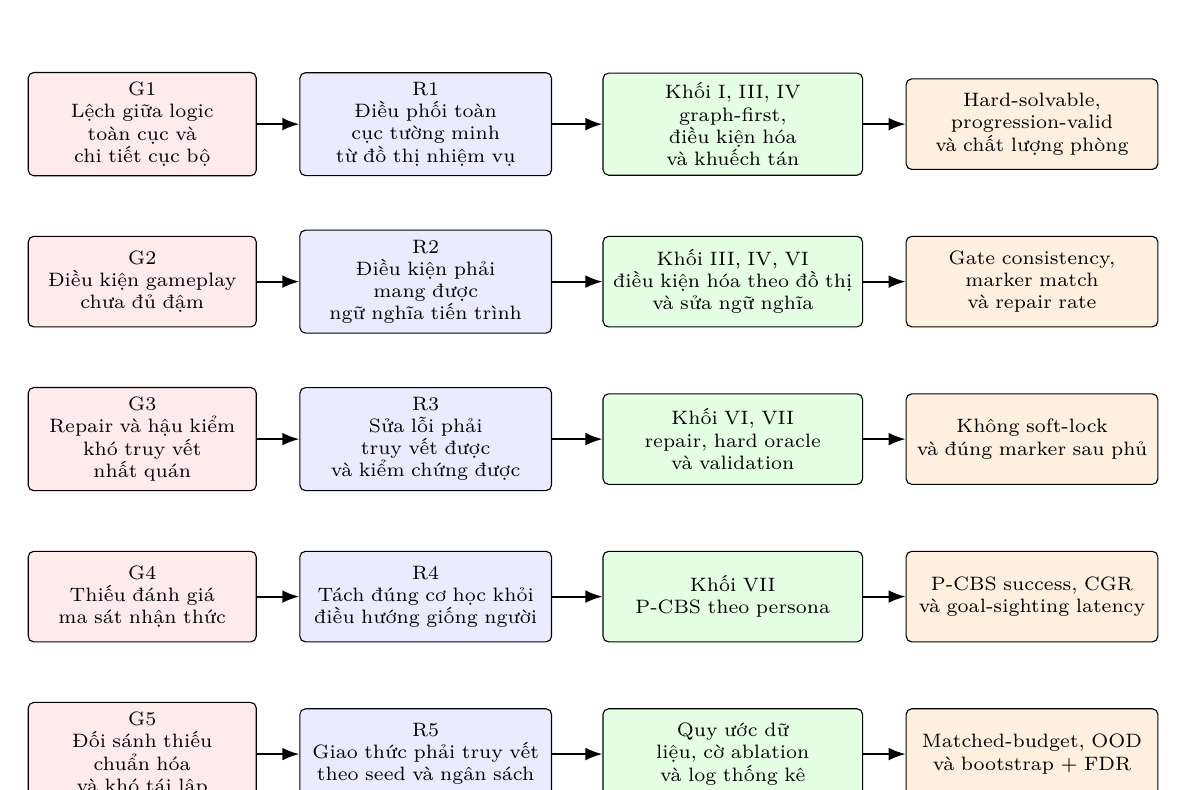
\begin{tikzpicture}[
  font=\scriptsize,
  >=Latex,
  boxgap/.style={draw, rounded corners=2pt, fill=red!8, align=center, text width=2.65cm, minimum height=1.15cm, inner sep=3.5pt},
  boxreq/.style={draw, rounded corners=2pt, fill=blue!8, align=center, text width=2.95cm, minimum height=1.15cm, inner sep=3.5pt},
  boxblk/.style={draw, rounded corners=2pt, fill=green!10, align=center, text width=3.05cm, minimum height=1.15cm, inner sep=3.5pt},
  boxmet/.style={draw, rounded corners=2pt, fill=orange!12, align=center, text width=2.95cm, minimum height=1.15cm, inner sep=3.5pt},
  arr/.style={->, line width=0.7pt}
]
\node[boxgap] (g1) at (0,0) {G1\\Lệch giữa logic toàn cục và\\chi tiết cục bộ};
\node[boxreq] (r1) at (3.6,0) {R1\\Điều phối toàn cục tường minh\\từ đồ thị nhiệm vụ};
\node[boxblk] (b1) at (7.5,0) {Khối I, III, IV\\graph-first, điều kiện hóa\\và khuếch tán};
\node[boxmet] (m1) at (11.3,0) {Hard-solvable, progression-valid\\và chất lượng phòng};

\node[boxgap] (g2) at (0,-2.0) {G2\\Điều kiện gameplay\\chưa đủ đậm};
\node[boxreq] (r2) at (3.6,-2.0) {R2\\Điều kiện phải mang được\\ngữ nghĩa tiến trình};
\node[boxblk] (b2) at (7.5,-2.0) {Khối III, IV, VI\\điều kiện hóa theo đồ thị\\và sửa ngữ nghĩa};
\node[boxmet] (m2) at (11.3,-2.0) {Gate consistency, marker match\\và repair rate};

\node[boxgap] (g3) at (0,-4.0) {G3\\Repair và hậu kiểm\\khó truy vết nhất quán};
\node[boxreq] (r3) at (3.6,-4.0) {R3\\Sửa lỗi phải truy vết được\\và kiểm chứng được};
\node[boxblk] (b3) at (7.5,-4.0) {Khối VI, VII\\repair, hard oracle\\và validation};
\node[boxmet] (m3) at (11.3,-4.0) {Không soft-lock\\và đúng marker sau phủ};

\node[boxgap] (g4) at (0,-6.0) {G4\\Thiếu đánh giá\\ma sát nhận thức};
\node[boxreq] (r4) at (3.6,-6.0) {R4\\Tách đúng cơ học khỏi\\điều hướng giống người};
\node[boxblk] (b4) at (7.5,-6.0) {Khối VII\\P-CBS theo persona};
\node[boxmet] (m4) at (11.3,-6.0) {P-CBS success, CGR\\và goal-sighting latency};

\node[boxgap] (g5) at (0,-8.0) {G5\\Đối sánh thiếu chuẩn hóa\\và khó tái lập};
\node[boxreq] (r5) at (3.6,-8.0) {R5\\Giao thức phải truy vết\\theo seed và ngân sách};
\node[boxblk] (b5) at (7.5,-8.0) {Quy ước dữ liệu, cờ ablation\\và log thống kê};
\node[boxmet] (m5) at (11.3,-8.0) {Matched-budget, OOD\\và bootstrap + FDR};

\draw[arr] (g1) -- (r1); \draw[arr] (r1) -- (b1); \draw[arr] (b1) -- (m1);
\draw[arr] (g2) -- (r2); \draw[arr] (r2) -- (b2); \draw[arr] (b2) -- (m2);
\draw[arr] (g3) -- (r3); \draw[arr] (r3) -- (b3); \draw[arr] (b3) -- (m3);
\draw[arr] (g4) -- (r4); \draw[arr] (r4) -- (b4); \draw[arr] (b4) -- (m4);
\draw[arr] (g5) -- (r5); \draw[arr] (r5) -- (b5); \draw[arr] (b5) -- (m5);
\end{tikzpicture}
}
\caption{Ánh xạ từ khoảng trống nghiên cứu sang yêu cầu thiết kế, khối phương pháp và các thước đo kiểm chứng.}
\label{fig:traceability_gap_design_metrics}
\end{figure}

\paragraph{Bảng ký hiệu cốt lõi cho Chương 3.}
Để giảm tải chuyển ngữ cảnh giữa các mục, Bảng~\ref{tab:core_notation_ch3} gom các ký hiệu được dùng lặp lại trong phần phương pháp.

\begin{table}[H]
\centering
\caption{Ký hiệu dùng xuyên suốt Chương 3}
\label{tab:core_notation_ch3}
\begin{tabular}{>{\raggedright\arraybackslash}p{2.2cm} >{\raggedright\arraybackslash}p{10.6cm}}
\toprule
Ký hiệu & Ý nghĩa \\
\midrule
$\mathcal{A}$ & Đồ thị kiến trúc ở mức hệ thống (khối xử lý và luồng dữ liệu). \\
$G$ & Đồ thị nhiệm vụ ở mức nội dung dungeon (tiến trình nhiệm vụ, lock--key, nhánh, mục tiêu). \\
$x_i$ & Lưới tile của phòng $i$ trong không gian rời rạc $16\times 11$. \\
$z_i$ & Biểu diễn latent của phòng $i$ trong không gian liên tục do VQ-VAE mã hóa. \\
$c_i$ & Vector điều kiện từ đồ thị sang phòng của phòng $i$ sau khi hợp nhất nhánh cục bộ và toàn cục. \\
$D$ & Dungeon đầu ra sau bước ghép phòng và hậu kiểm tra ký hiệu. \\
$(f,v,\phi)$ & Bộ chẩn đoán cá thể đồ thị gồm fitness, mức vi phạm ràng buộc và cờ khả thi. \\
$\mathcal{L}_{\mathrm{diff}},\mathcal{L}_{\mathrm{logic}}$ & Thành phần mất mát chính trong huấn luyện khuếch tán có điều kiện và hướng dẫn logic. \\
$\mathbb{I}_{\mathrm{fallback}}$ & Biến chỉ thị kích hoạt bước quay về mô hình giáo viên trong suy luận phòng. \\
$U(a)$ & Hàm tiện ích dùng trong P-CBS để xếp hạng trạng thái-kế tiếp ở tầng xác nhận hành vi giới hạn nhận thức. \\
$\mathrm{CGR}$ & Tỉ lệ \emph{cognitive gap}: phần trăm trường hợp bộ kiểm tra cơ học xác nhận giải được nhưng P-CBS thất bại. \\
\bottomrule
\end{tabular}
\end{table}

\section{Kiến trúc tổng thể và quy ước dữ liệu}

\subsection{Phân biệt đồ thị kiến trúc và đồ thị nhiệm vụ}
Để tránh nhập nhằng thuật ngữ, chương này dùng song song hai lớp đồ thị có vai trò khác nhau:
\begin{equation}
\mathcal{A}=(V_{\mathcal{A}},E_{\mathcal{A}}),
\qquad
G=(V_G,E_G).
\end{equation}
Trong đó $\mathcal{A}$ là \emph{đồ thị kiến trúc} ở mức hệ thống (nút là các khối xử lý, cạnh là luồng dữ liệu/chỉ đạo), còn $G$ là \emph{đồ thị nhiệm vụ} ở mức nội dung dungeon (nút là phòng/trạng thái nhiệm vụ, cạnh là quan hệ tiến trình gameplay) \cite{dormans2011missionspaces}. Khối I có thể sinh mới $G$ bằng tiến hóa; các khối còn lại nhận $G$ để điều kiện hóa sinh phòng, sửa lỗi, và đánh giá chất lượng.

\paragraph{Quy ước thuật ngữ cho Chương 3.}
Trong chương này, thuật ngữ \emph{graph} được dùng chủ yếu theo nghĩa đồ thị
nhiệm vụ trong mission-space PCG, tức cấu trúc liên thông cùng các quan hệ tiến
trình có ràng buộc như lock--key, item-gate, switch-state và boss gate
\cite{dormans2011missionspaces,mota2021dungeon,togelius2011pcg}. Khi chỉ phân
tích hình thái đồ thị, chẳng hạn số nút, số cạnh, hệ số phân nhánh, chu trình
hay phân lớp topo, văn bản dùng cụm sinh cấu trúc đồ thị như một tên gọi rút
gọn \cite{kahn1962topological}. Trong khóa luận này, cụm \emph{topo} chỉ được dùng
theo nghĩa \emph{thứ tự topo} hoặc \emph{phân lớp topo} trên đồ thị có hướng không
chu trình; khóa luận không dùng \emph{topology} theo nghĩa không gian topo của toán học
để mô tả dungeon. Khi nhấn mạnh thứ tự mở tiến trình và điều kiện
vượt ải, văn bản dùng các cụm ngữ nghĩa tiến trình hoặc ràng buộc tiến trình
nhiệm vụ để cho thấy đây là lớp ngữ nghĩa gameplay rộng hơn nghĩa đồ thị thuần
túy trong lý thuyết đồ thị. Vì vậy, cách gọi đầy đủ cho Khối I trong ngữ cảnh
phương pháp là sinh cấu trúc và ngữ nghĩa tiến trình của đồ thị nhiệm vụ, còn
\emph{graph generation} chỉ được dùng ở những đoạn mô tả thuần hình thái cấu
trúc.

\subsection{Mô hình đồ thị kiến trúc 7 khối}
Để đặc tả kiến trúc ở mức cấu trúc, ta mô hình hóa toàn quy trình bằng một đồ thị có hướng:
\begin{equation}
\mathcal{A}=(V_{\mathcal{A}},E_{\mathcal{A}}),
\qquad
V_{\mathcal{A}}=\{B_1,\ldots,B_7\},
\end{equation}
trong đó $B_1$ đến $B_7$ lần lượt tương ứng các khối I đến VII ở Hình~\ref{fig:architecture_7blocks}. Tập cạnh được tách thành hai phần:
\begin{equation}
E_{\mathcal{A}}=E_{\text{core}}\cup E_{\text{opt}},
\end{equation}
với $E_{\text{core}}$ là các luồng bắt buộc trên đường chạy chính (cấu trúc đồ thị nhiệm vụ $\rightarrow$ điều kiện hóa $\rightarrow$ khuếch tán $\rightarrow$ sửa lỗi), còn $E_{\text{opt}}$ là các luồng tùy chọn dùng cho hướng dẫn logic hoặc đánh giá chất lượng--đa dạng.

Ở mức hiện thực, trục định lượng của khóa luận bám theo đường chạy chính gồm bảy khối chức năng của hệ thống. Luồng này nối liền các bước thích nghi dữ liệu, sinh đồ thị nhiệm vụ, VQ-VAE ngữ nghĩa, mã hóa điều kiện, khuếch tán tiềm ẩn, LogicNet, symbolic refiner và tầng hậu kiểm. Một số tiện ích triển khai bổ sung như làm mịn mép ghép, kiểm tra va chạm, ghi demo hay giải thích quyết định chỉ đóng vai trò hỗ trợ vận hành; chúng không được dùng làm cơ sở cho các tuyên bố định lượng ở Chương~4. Cách neo mô tả như vậy giúp Chương~3 bám đúng hiện thực của hệ thống, đồng thời giữ cho Chương~4 chỉ phản ánh những thành phần thật sự đi vào giao thức thực nghiệm chính.

\begin{figure}[H]
\centering
\resizebox{0.92\linewidth}{!}{%
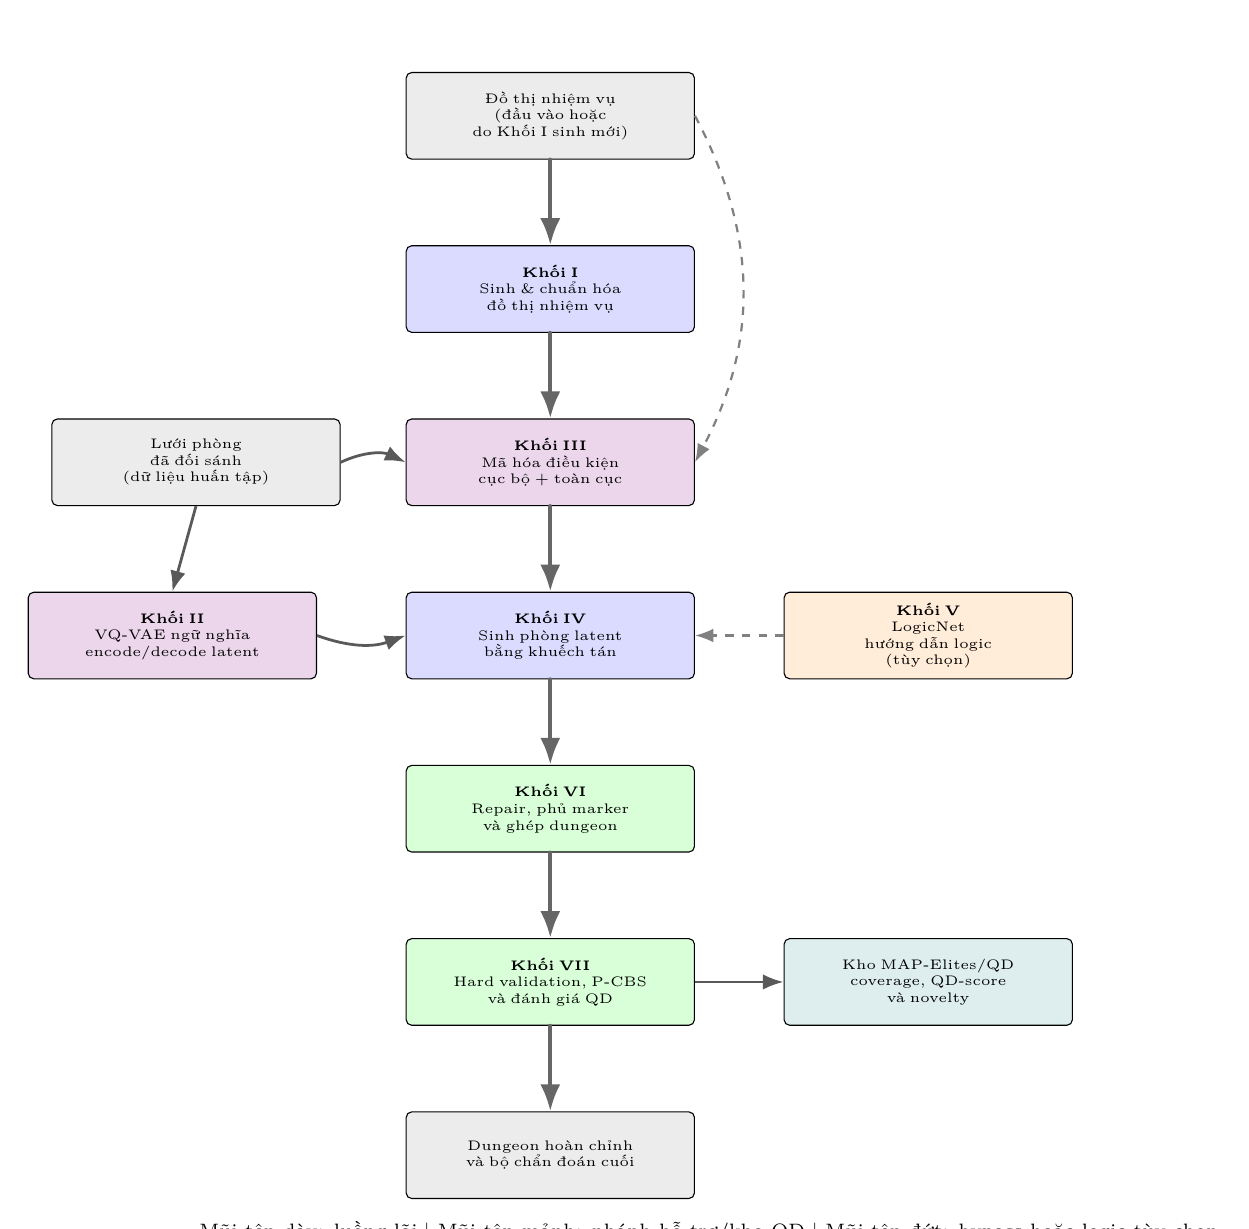
\begin{tikzpicture}[
  font=\tiny,
  >=Latex,
  io/.style={draw, rounded corners=2pt, fill=gray!15, align=center, text width=3.45cm, minimum height=1.1cm, inner sep=3pt, font=\tiny},
  block/.style={draw, rounded corners=2pt, fill=blue!14, align=center, text width=3.45cm, minimum height=1.1cm, inner sep=3pt, font=\tiny},
  latent/.style={draw, rounded corners=2pt, fill=violet!16, align=center, text width=3.45cm, minimum height=1.1cm, inner sep=3pt, font=\tiny},
  guide/.style={draw, rounded corners=2pt, fill=orange!15, align=center, text width=3.45cm, minimum height=1.1cm, inner sep=3pt, font=\tiny},
  post/.style={draw, rounded corners=2pt, fill=green!15, align=center, text width=3.45cm, minimum height=1.1cm, inner sep=3pt, font=\tiny},
  archive/.style={draw, rounded corners=2pt, fill=teal!13, align=center, text width=3.45cm, minimum height=1.1cm, inner sep=3pt, font=\tiny},
  core_arr/.style={->, line width=1.5pt, color=black!60, line cap=round},
  branch_arr/.style={->, line width=1.0pt, color=black!65},
  opt_arr/.style={->, line width=0.8pt, color=black!50, dashed}
]
  % Core pipeline (vertical center) - compact spacing
  \node[io] (graphin) at (0,0) {Đồ thị nhiệm vụ\\(đầu vào hoặc\\do Khối I sinh mới)};
  \node[block] (b1) at (0,-2.2) {\textbf{Khối I}\\Sinh \& chuẩn hóa\\đồ thị nhiệm vụ};
  \node[latent] (b3) at (0,-4.4) {\textbf{Khối III}\\Mã hóa điều kiện\\cục bộ + toàn cục};
  \node[block] (b4) at (0,-6.6) {\textbf{Khối IV}\\Sinh phòng latent\\bằng khuếch tán};
  \node[post] (b6) at (0,-8.8) {\textbf{Khối VI}\\Repair, phủ marker\\và ghép dungeon};
  \node[post] (b7) at (0,-11.0) {\textbf{Khối VII}\\Hard validation, P-CBS\\và đánh giá QD};
  \node[io] (out) at (0,-13.2) {Dungeon hoàn chỉnh\\và bộ chẩn đoán cuối};

  % Left branch: representation learning
  \node[io] (roomdata) at (-4.5,-4.4) {Lưới phòng\\đã đối sánh\\(dữ liệu huấn tập)};
  \node[latent] (b2) at (-4.8,-6.6) {\textbf{Khối II}\\VQ-VAE ngữ nghĩa\\encode/decode latent};

  % Right branch: logic guidance
  \node[guide] (b5) at (4.8,-6.6) {\textbf{Khối V}\\LogicNet\\hướng dẫn logic\\(tùy chọn)};
  \node[archive] (qdarchive) at (4.8,-11.0) {Kho MAP-Elites/QD\\coverage, QD-score\\và novelty};

  % Main core pipeline arrows
  \draw[core_arr] (graphin.south) -- (b1.north);
  \draw[core_arr] (b1.south) -- (b3.north);
  \draw[core_arr] (b3.south) -- (b4.north);
  \draw[core_arr] (b4.south) -- (b6.north);
  \draw[core_arr] (b6.south) -- (b7.north);
  \draw[core_arr] (b7.south) -- (out.north);
  \draw[opt_arr, bend left=28] (graphin.east) to (b3.east);

  % Left branch (supporting data flow)
  \draw[branch_arr] (roomdata.south) -- (b2.north);
  \draw[branch_arr, bend left=25] (roomdata.east) to (b3.west);
  \draw[branch_arr, bend right=20] (b2.east) to (b4.west);

  % Right branch (optional logic signal)
  \draw[opt_arr] (b5.west) -- (b4.east);
  \draw[branch_arr] (b7.east) -- (qdarchive.west);

  % Label for flow types
  \node[anchor=north west, font=\scriptsize, inner sep=1pt] at (-4.5, -14.0) {
    Mũi tên dày: luồng lõi $|$ Mũi tên mảnh: nhánh hỗ trợ/kho QD $|$ Mũi tên đứt: bypass hoặc logic tùy chọn
  };
\end{tikzpicture}
}
\caption{Kiến trúc bảy khối của quy trình sinh lai nơ-ron. Mũi tên dày là luồng lõi từ đồ thị nhiệm vụ đến dungeon hoàn chỉnh; mũi tên mảnh là nhánh hỗ trợ và cập nhật kho MAP-Elites/QD; mũi tên đứt là bypass khi đồ thị nhiệm vụ được cung cấp sẵn hoặc tín hiệu logic tùy chọn.}
\label{fig:architecture_7blocks}
\end{figure}

Trong phân rã chức năng, Khối I không chỉ sinh mà còn chuẩn hóa và hậu kiểm đồ thị nhiệm vụ trước khi giao cho các tầng sau; Khối II học không gian mã rời rạc bằng VQ-VAE; Khối III hợp nhất điều kiện cục bộ và toàn cục theo đồ thị; Khối IV lấy mẫu trong không gian tiềm ẩn; Khối V bổ sung tín hiệu logic khả vi khi được bật; Khối VI đảm nhiệm repair ký hiệu, phủ marker và ghép dungeon; còn Khối VII chốt vòng kiểm tra đúng luật chơi, thẩm định theo persona bằng P-CBS và cập nhật các chỉ số chất lượng--đa dạng ở mức dungeon. Cách tách khối này tạo ra ranh giới đủ rõ để Chương 4 có thể đo đóng góp biên của từng thành phần.

Đối chiếu với hiện thực hệ thống cho thấy ánh xạ bảy khối ở Hình~\ref{fig:architecture_7blocks} là nhất quán với đường chạy chuẩn trong mã nguồn: Khối I sinh và hợp lệ hóa mission graph, Khối II học biểu diễn rời rạc bằng VQ-VAE, Khối III hợp nhất điều kiện cục bộ và toàn cục theo đồ thị, Khối IV sinh latent bằng khuếch tán, Khối V cung cấp tín hiệu logic khả vi, Khối VI thực hiện symbolic repair cùng các bước phủ marker/ghép dungeon, và Khối VII đảm nhiệm kiểm tra cơ học, thẩm định P-CBS và cập nhật kho MAP-Elites/QD. Các thành phần vận hành phụ trợ được tách riêng và không dùng làm cơ sở cho tuyên bố định lượng.

Quan trọng hơn, Hình~\ref{fig:architecture_7blocks} cũng làm rõ ranh giới giữa các luồng vận hành. Đường lõi là luồng bắt buộc khi hệ thống tạo một dungeon mới: nhận hoặc sinh đồ thị nhiệm vụ, tạo điều kiện từ đồ thị sang phòng, lấy mẫu latent, sửa lỗi ký hiệu rồi mới ghép dungeon để đánh giá. Đường dưới gom các thành phần nền và hậu sinh: dữ liệu phòng dùng để học biểu diễn ở Khối II; Khối II cung cấp không gian latent cho Khối IV ở cả huấn luyện lẫn suy luận; Khối V chỉ xuất hiện khi bật hướng dẫn logic; còn Khối VII chỉ được gọi sau khi dungeon đã ghép xong và chỉ cập nhật kho QD khi mẫu vượt qua điều kiện kiểm tra. Nhờ vậy, sơ đồ không chỉ cho biết thứ tự các khối mà còn cho thấy khối nào thuộc luồng lõi, khối nào là nhánh hỗ trợ hoặc hậu kiểm.

\subsection{Ma trận đầu vào, đầu ra và kiểm soát lỗi theo khối}
Để truy vết được trách nhiệm của từng khối trong đường chạy chính, Bảng~\ref{tab:block_contract_matrix} tóm tắt đầu vào, đầu ra, bước kiểm soát lỗi và nhóm chỉ số giám sát tương ứng.

\begin{longtable}{>{\raggedright\arraybackslash}p{0.9cm} >{\raggedright\arraybackslash}p{5.1cm} >{\raggedright\arraybackslash}p{3.8cm} >{\raggedright\arraybackslash}p{3.8cm}}
\caption{Ma trận đầu vào, đầu ra và kiểm soát lỗi theo từng khối}
\label{tab:block_contract_matrix}\\
\toprule
Khối & Đầu vào, đầu ra cốt lõi & Kiểm soát lỗi và chuyển trạng thái & Mục tiêu hoặc chỉ số chính \\
\midrule
\endfirsthead
\toprule
Khối & Đầu vào, đầu ra cốt lõi & Kiểm soát lỗi và chuyển trạng thái & Mục tiêu hoặc chỉ số chính \\
\midrule
\endhead
$B_1$ & Vào: luật, seed, hồ sơ ràng buộc. Ra: đồ thị nhiệm vụ khả thi $G$ và bộ mô tả cấu trúc/tiến trình. & Chọn nghiệm khả thi-ưu tiên; hậu kiểm tra liên thông, start-goal, virtual node. & Fitness đa mục tiêu, mức vi phạm $v$, cờ khả thi $\phi$. \\
$B_2$ & Vào: lưới phòng rời rạc. Ra: latent $z$ và giải mã tile. & Kiểm tra kích thước chuẩn, loại các lô chứa giá trị không hữu hạn. & $\mathcal{L}_{\mathrm{recon}}$, $\mathcal{L}_{\mathrm{VQ}}$, tỷ lệ tile hiếm. \\
$B_3$ & Vào: $(X,E_{idx},E_f,\mathrm{TPE})$ cùng latent lân cận. Ra: điều kiện phòng $c_i$. & Kiểm tra lược đồ tensor và dừng sớm khi sai kích thước. & Độ ổn định điều kiện hóa theo lớp phòng, lỗi lược đồ bằng 0. \\
$B_4$ & Vào: $z_t$, timestep $t$, điều kiện $c$. Ra: latent mẫu và dự đoán nhiễu/vận tốc. & Kẹp CFG theo miền chưng cất, trọng số Min-SNR, cắt gradient. & $\mathcal{L}_{\mathrm{diff}}$, tốc độ mẫu sinh, tỷ lệ quay về mô hình giáo viên. \\
$B_5$ & Vào: latent trung gian và plan trace. Ra: gradient logic và $\mathcal{L}_{\mathrm{logic}}$. & Warmup theo epoch; tắt logic khi thành phần không khả dụng. & Grid reach, trace consistency, anchor consistency. \\
$B_6$ & Vào: lưới nơ-ron, mặt nạ kế hoạch, marker đồ thị. Ra: lưới phòng đã sửa và hợp lệ biên-cửa. & Ép biên, sửa có dẫn dắt bởi WFC, giới hạn số vòng sửa. & Repair rate, số lỗi cửa/đảo, hợp lệ kích thước phòng. \\
$B_7$ & Vào: dungeon đã ghép và lưới hậu sinh đã chuẩn hóa. Ra: phán quyết cơ học, chỉ số P-CBS, cập nhật kho QD và thống kê hậu sinh. & Chuẩn hóa lưới ghép, loại bỏ token ngoài bảng từ điển/\texttt{VOID} nội suy, ép đúng một start-goal, chỉ thêm vào kho khi bài kiểm tra cơ học vượt qua. & Hard-solvable rate, cognitive-gap rate, navigation entropy/confusion, coverage, QD-score. \\
\bottomrule
\end{longtable}

\subsection{Dòng chảy đầu-cuối của quy trình}
Gọi $G$ là đồ thị nhiệm vụ, $N$ là số phòng vật lý sau bước lọc nút ảo và $D$ là dungeon đầu ra. Hệ thống thực hiện ánh xạ:
\begin{equation}
D = \mathcal{S}\Big(\{\,\mathcal{R}(\mathcal{N}(C_i, G_i))\,\}_{i=1}^{N}\Big),
\end{equation}
trong đó $\mathcal{N}$ là khối sinh phòng nơ-ron có điều kiện, $\mathcal{R}$ là khối sửa lỗi ký hiệu theo ràng buộc cục bộ, và $\mathcal{S}$ là khối ghép phòng để tạo bản đồ toàn cục.

Trong thực thi, quy trình gồm ba lớp xử lý nối tiếp. Ở lớp đồ thị, hệ thống hoặc nhận đồ thị nhiệm vụ từ đầu vào hoặc tự sinh cấu trúc đồ thị nhiệm vụ bằng tìm kiếm tiến hóa, rồi chuẩn hóa thứ tự nút để cố định ánh xạ giữa định danh phòng và chỉ số nút. Ở lớp phòng, các phòng được sinh theo lớp topo của đồ thị có hướng \cite{kahn1962topological}, sau đó nhóm theo dạng latent để gom lô mà không phá phụ thuộc tiền nhiệm. Ở lớp hậu xử lý, đầu ra nơ-ron được kiểm tra và sửa cục bộ theo mặt nạ kế hoạch trước khi ghép dungeon, nhờ đó tính nhất quán tiến trình được bảo toàn khi chuyển từ mức phòng sang mức toàn bản đồ.

\subsection{Biểu diễn dữ liệu và lược đồ đầu vào}
Đồ thị nhiệm vụ được biểu diễn dưới hai dạng: vô hướng để duy trì liên thông toàn cục và có hướng để mô tả phụ thuộc tiến trình. Từ đồ thị này, hệ thống trích xuất tensor đặc trưng nút 14 chiều, đặc trưng cạnh 16 chiều và mã hóa vị trí theo thứ tự topo 8 chiều. Không gian phòng sử dụng lưới rời rạc $16\times 11$ với 44 lớp tile; sau đó Khối II ánh xạ sang latent chuẩn hóa $64\times 4\times 3$ thông qua VQ-VAE \cite{oord2017vqvae}. Thiết kế ở mức latent giúp diffusion học phân bố ổn định hơn trong thiết lập dữ liệu phòng quy mô nhỏ, đồng thời vẫn duy trì khả năng can thiệp ký hiệu ở tầng tile \cite{rombach2022ldm}.
Ở mức hiện thực, quy ước dữ liệu từ đồ thị sang phòng không chỉ được neo bởi số chiều tensor mà còn bởi ý nghĩa của từng nhóm đặc trưng. Bảng~\ref{tab:graph_room_contract} tóm tắt lược đồ tín hiệu được dùng nhất quán giữa bước nạp dữ liệu, huấn luyện, suy luận và thẩm định; nhờ đó các khối không chỉ tương thích về kích thước mà còn bảo toàn đúng ngữ nghĩa gameplay khi chuyển dữ liệu qua từng tầng.

\begin{table}[H]
\centering
\caption{Lược đồ dữ liệu từ đồ thị sang phòng được dùng xuyên suốt huấn luyện và suy luận}
\label{tab:graph_room_contract}
\footnotesize
\begin{tabular}{>{\raggedright\arraybackslash}p{2.1cm} >{\raggedright\arraybackslash}p{2.7cm} >{\raggedright\arraybackslash}p{8.1cm}}
\toprule
Nhóm tensor & Kích thước & Thành phần ngữ nghĩa chính \\
\midrule
$X$ & $N\times 14$ & 6 tín hiệu vai trò/chức năng (enemy, key, item, goal, boss, puzzle), 4 tín hiệu đếm đã chuẩn hóa (enemy, key, item, puzzle), difficulty, cờ start, cờ secret và cờ hub. \\
$E_f$ & $M\times 16$ & 8 tín hiệu nền/cổng (open, key-lock, bombable, soft-lock, boss-lock, item-lock, stair/warp, switch/state) và 8 tín hiệu mở rộng (hazard, shutter, hidden, one-way tiến/lùi, multi-lock, state-block hoặc switch-count, battery/group). \\
$\mathrm{TPE}$ & $N\times 8$ & Khoảng cách chuẩn hóa từ start và đến goal, bậc nút, cờ nằm trên đường chính, tín hiệu liên quan key/lock, difficulty cục bộ và dấu vết phụ thuộc khóa. \\
$\mathbf{B}_{\text{cond}}$ & $B\times 8$ & Ràng buộc biên theo thứ tự $[h_N,r_N,h_S,r_S,h_E,r_E,h_W,r_W]$. \\
$\mathbf{T}_{\text{topo}}$ & $B\times 54\times 16\times 11$ & 11 kênh nền (traversability, start, goal, cửa và generic gated theo 4 hướng), 32 kênh cổng có kiểu từ 8 họ ràng buộc $\times$ 4 hướng, và 11 kênh vai trò phòng. Khi bật chế độ puzzle-stage, stage trace được rasterize vào kênh traversability thay vì làm thay đổi bề rộng tensor. \\
\bottomrule
\end{tabular}
\end{table}

Vì vậy, mọi thí nghiệm loại trừ hoặc thay thế mô-đun trong khóa luận đều phải bảo toàn đồng thời thứ tự đặc trưng, bề rộng tensor và quy ước chuẩn hóa; nếu không, sai lệch sẽ xuất hiện ở tầng ngữ nghĩa gameplay trước khi lộ ra ở tầng chỉ số.
Chi tiết cách hợp nhất điều kiện cục bộ và toàn cục của Khối III được trình bày riêng trong Mục 3.3 để tách bạch lớp quy ước dữ liệu và lớp thiết kế thuật toán của từng khối.

\subsection{Nguồn dữ liệu, tiền xử lý và chia tập}
Nguồn dữ liệu của khóa luận là corpus Zelda được tổ chức trong thư mục dữ liệu của dự án từ hai lớp nguồn bổ sung nhau: bản đồ dungeon gốc của \textit{The Legend of Zelda} lấy từ bộ sưu tập Nintendo Maps của Rick Bruns \cite{brunsNesMapsZelda}, và lớp biểu diễn ký hiệu hóa ở mức tile được chuẩn hóa theo tinh thần của VGLC cùng văn liệu PCGML trên game \cite{summerville2016vglc,summerville2018pcgml}. Trên nền đó, dự án số hóa thêm đồ thị nhiệm vụ để nối hình học dungeon với tiến trình gameplay, phù hợp với hướng tách cấu trúc liên thông cấp dungeon và hiện thực hóa phòng trong các nghiên cứu Zelda trước đây \cite{summerville2015zelda,summerville2015samplinghyrule}. Toàn bộ corpus hiện gồm $18$ dungeon gốc, tương ứng $9$ level của Quest~1 và $9$ biến thể Quest~2. Mỗi dungeon đi kèm ba lớp tư liệu: bản đồ ảnh ở mức toàn dungeon, lưới tile ASCII đã chuẩn hóa và đồ thị nhiệm vụ đã số hóa kèm bộ từ điển nhãn nút/cạnh dùng để diễn giải vai trò phòng và loại cổng. Kích thước lưới gốc thay đổi từ $32\times 88$ đến $128\times 88$. Bộ từ điển quan hệ hiện có $9$ nhãn nút và $7$ nhãn cạnh, đủ để biểu diễn các vai trò cơ bản như start, key, boss, puzzle, triforce cùng các quan hệ mở khóa như key-locked, bombable, boss-key-locked, item-locked, soft-locked và switch-locked.

Sau bước đối sánh giữa lưới phòng và đồ thị nhiệm vụ, hệ thống trích được $459$ mẫu phòng để huấn luyện ở mức phòng. Bảng~\ref{tab:dataset_examples} cho ba ví dụ tiêu biểu lấy trực tiếp từ corpus nguồn, đại diện cho ba dải quy mô nhỏ, trung bình và lớn.

\begin{table}[H]
\centering
\caption{Ba dải quy mô tiêu biểu trong corpus Zelda đã chuẩn hóa}
\label{tab:dataset_examples}
\footnotesize
\begin{tabular}{>{\raggedright\arraybackslash}p{2.45cm} >{\centering\arraybackslash}p{2.0cm} >{\centering\arraybackslash}p{1.5cm} >{\centering\arraybackslash}p{2.0cm} >{\raggedright\arraybackslash}p{4.6cm}}
\toprule
Nhóm mẫu & Lưới gốc & Số phòng & Nút/cạnh đồ thị & Nhận xét ngắn \\
\midrule
Quy mô nhỏ & $32\times 88$ & 14 & 16 / 32 & Ít nhánh, mật độ cổng thấp, phù hợp để kiểm tra đường cơ sở và các điều kiện tiến trình ngắn. \\
Quy mô trung bình & $64\times 88$ & 30 & 35 / 82 & Có nhiều nút chức năng và nhiều chỗ rẽ, tạo áp lực rõ lên điều kiện hóa theo đồ thị và sửa lỗi hậu kỳ. \\
Quy mô lớn & $128\times 88$ & 57 & 62 / 144 & Cấu trúc sâu và dày, giàu cổng và nhánh vòng, thích hợp để đo suy luận nhiều bước và hậu kiểm toàn dungeon. \\
\bottomrule
\end{tabular}
\end{table}

Để người đọc thấy trực tiếp ba dạng dữ liệu mà quy trình khai thác, Hình~\ref{fig:zelda_data_modalities} minh họa cùng một dungeon qua ba lớp biểu diễn: bản đồ ảnh gốc, đồ thị nhiệm vụ sau số hóa và trích đoạn văn bản đã chuẩn hóa. Chuỗi này cũng phản ánh đúng thứ tự tiền xử lý của hệ thống: bắt đầu từ bản đồ nguyên gốc, dựng đồ thị nhiệm vụ để cố định ngữ nghĩa tiến trình, rồi mới tách phòng và đưa về biểu diễn ký hiệu phục vụ huấn luyện.

\begin{figure}[H]
\centering
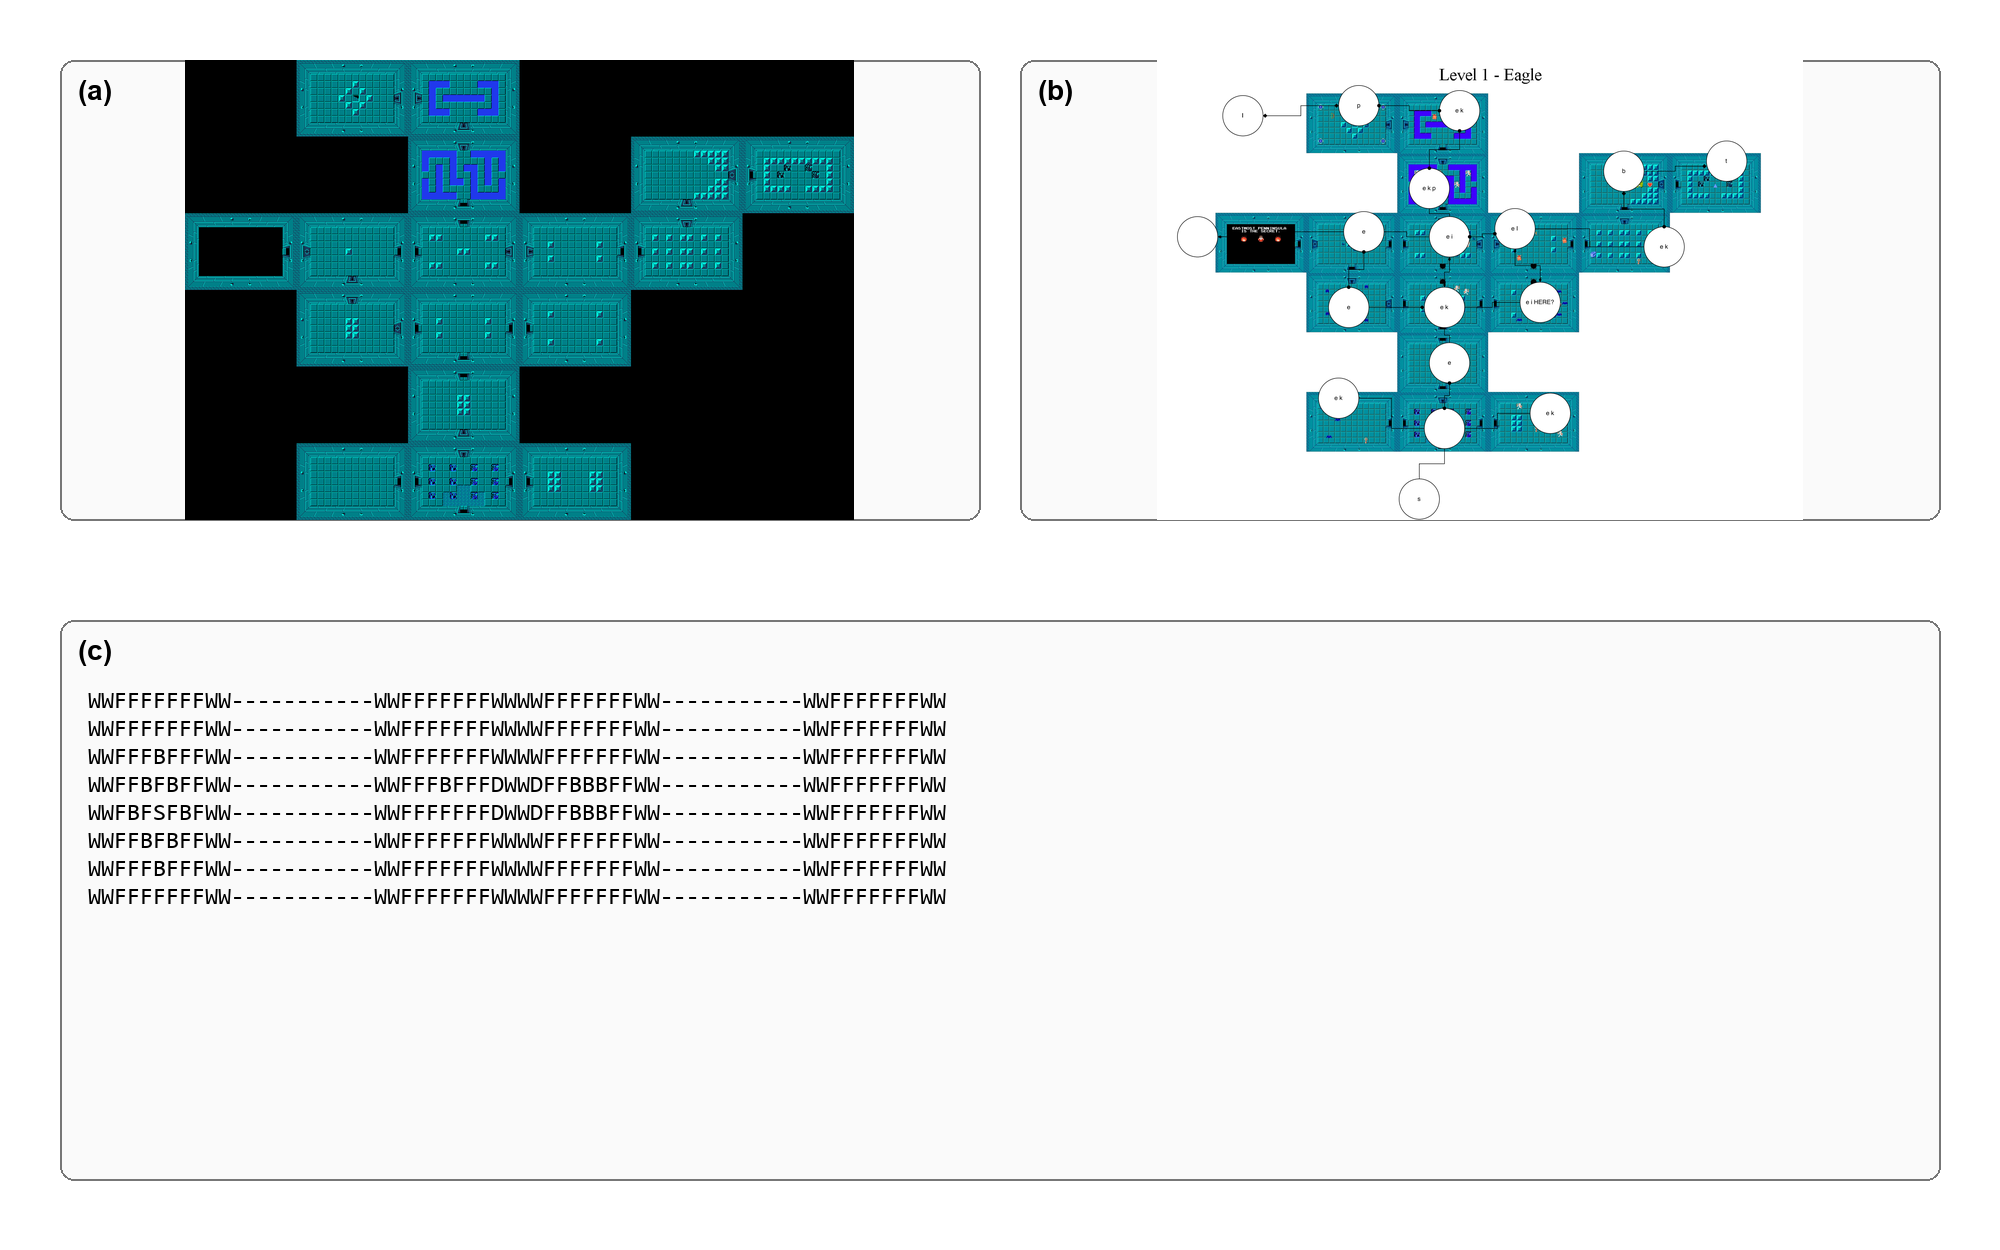
\includegraphics[width=\linewidth]{figures/data/zelda_data_modalities.png}
\caption{Ba dạng dữ liệu được dùng đồng thời trong quy trình sinh Zelda. (a) Bản đồ dungeon gốc. (b) Đồ thị nhiệm vụ sau bước số hóa, được chồng lên bản đồ để kiểm tra sự khớp nhau giữa hình học và tiến trình. (c) Trích đoạn biểu diễn ASCII sau chuẩn hóa, trong đó mỗi ký hiệu mã hóa trực tiếp một lớp tile hoặc vùng rỗng.}
\label{fig:zelda_data_modalities}
\end{figure}

Trong quy trình thực nghiệm, ba dạng dữ liệu này đảm nhiệm ba vai trò khác nhau. Bản đồ ảnh được giữ lại để đối chiếu trực quan và kiểm tra bước số hóa. Biểu diễn ASCII là miền làm việc gọn nhẹ cho bước tách phòng, chuẩn hóa tile và dựng mẫu huấn luyện. Đồ thị nhiệm vụ đóng vai trò mốc tham chiếu cho tiến trình, giúp phân biệt những phòng có hình học tương tự nhưng chức năng gameplay khác nhau. Ở nhánh văn bản, corpus dùng một bảng ký hiệu ASCII khá gọn cho tường, sàn, cửa, cầu thang, quái, khối đẩy, ô môi trường, hai kiểu ô ghép và khoảng trống \cite{summerville2016vglc,summerville2018pcgml}. Khi đưa vào quy trình, các ký hiệu này được ánh xạ vào bảng ngữ nghĩa chuẩn gồm $44$ mã tile để thống nhất với bước đặt dấu mốc tiến trình, phân loại cổng và sửa lỗi ký hiệu. Nhờ vậy, dữ liệu nguồn vẫn giữ được sự gọn nhẹ của biểu diễn VGLC, trong khi tầng sinh và tầng hậu kiểm có đủ chi tiết để mô tả các tình huống gameplay phong phú hơn.

\begin{table}[H]
\centering
\small
\caption{Bảng ký hiệu ASCII của corpus Zelda gốc}
\label{tab:ascii_symbol_legend}
\begin{tabular}{ll}
\toprule
Ký hiệu & Ý nghĩa \\
\midrule
\texttt{F} & Sàn đi được (\emph{floor}) \\
\texttt{B} & Khối chặn hoặc khối đẩy (\emph{block}) \\
\texttt{M} & Quái hoặc thực thể đối kháng (\emph{monster}) \\
\texttt{P} & Ô môi trường không đi được như lava hoặc water \\
\texttt{O} & Ô môi trường đặt trên sàn, vẫn giữ được mặt đi \\
\texttt{I} & Ô môi trường đặt trên khối, dùng cho vật cản đặc biệt \\
\texttt{D} & Cửa; loại cửa cụ thể được suy ra thêm từ đồ thị nhiệm vụ \\
\texttt{S} & Cầu thang, thang xuống hoặc warp \\
\texttt{W} & Tường \\
\texttt{-} & Khoảng trống ngoài dungeon (\emph{void}) \\
\bottomrule
\end{tabular}
\end{table}

Một trích đoạn ngắn trong Bảng~\ref{tab:ascii_symbol_legend} được cho ở
Liệt kê~\ref{lst:dataset_excerpt_ch3} để người đọc hình dung rõ đầu vào văn bản mà
quy trình thật sự nạp. Trong mã nguồn, mỗi phòng sau chuẩn hóa được lưu theo dạng ma
trận $(16,11)$, tức $16$ hàng và $11$ cột; đây là quy ước lưu trữ nội bộ theo
row-major của NumPy/PyTorch, khác với cách mô tả quen thuộc ``$16$ cột $\times 11$
hàng'' trong tài liệu Zelda nhưng không làm thay đổi nội dung hình học của phòng.

\begin{center}
\begin{minipage}{0.38\linewidth}
\begin{lstlisting}[caption={Trích đoạn ASCII ngắn từ corpus Zelda sau chuẩn hóa},label={lst:dataset_excerpt_ch3}]
WWWWWWWWWWW
WWFFFFFFFWW
WWFFFBFFFWW
WWFFBFBFFWW
WWFDFFFBFWW
WWFFFFFFFWW
WWWWWWWWWWW
\end{lstlisting}
\end{minipage}
\end{center}

Từ biểu diễn ký hiệu này, hệ thống dựng thêm một lớp quy tắc gameplay để đảm bảo hình
học phòng không tách rời tiến trình. Bảng~\ref{tab:core_game_rules_ch3} tóm tắt các
luật cốt lõi thật sự chi phối việc nạp dữ liệu, sinh phòng, ghép dungeon và hậu kiểm.
Những biến thể chi tiết hơn của luật và các bảng liệt kê dài hơn được đưa xuống phụ
lục để tránh làm đứt mạch trình bày của Chương~3.

\begin{table}[H]
\centering
\footnotesize
\caption{Các luật gameplay cốt lõi được dùng xuyên suốt trong quy trình}
\label{tab:core_game_rules_ch3}
\begin{tabular}{>{\raggedright\arraybackslash}p{2.8cm} >{\raggedright\arraybackslash}p{5.2cm} >{\raggedright\arraybackslash}p{5.8cm}}
\toprule
Nhóm luật & Nội dung chính & Vai trò trong quy trình \\
\midrule
Hợp lệ hình học phòng & Phòng phải có kích thước chuẩn $16\times 11$, mã tile hợp lệ và biên cửa khớp với phòng kề. & Loại lỗi sớm ở bước nạp dữ liệu, sửa biên và sửa ký hiệu sau sinh. \\
Liên thông dungeon & Dungeon sau ghép phải liên thông, có đúng một \texttt{START} và đúng một \texttt{TRIFORCE}. & Bảo đảm đầu ra có thể bước vào giai đoạn kiểm tra cơ học và P-CBS. \\
Khóa--cửa--vật phẩm & Cửa khóa thường cần chìa nhỏ, cửa boss cần \texttt{boss\_key}, cửa vật phẩm cần \texttt{key\_item}; tài nguyên chỉ được cộng một lần khi người chơi ghé phòng lần đầu. & Neo đúng thứ tự mở tiến trình trong bộ giải cơ học và trong P-CBS. \\
Cửa phá tường và cửa trạng thái & Cửa \texttt{bombable}, \texttt{switch} hay \texttt{state\_block} chỉ mở khi điều kiện tương ứng đã được thiết lập. & Ngăn các đường đi giả do mô hình sinh tạo ra nhưng không hợp lệ theo luật chơi. \\
Không soft-lock & Người chơi không được bị kẹt trong cấu hình không thể hoàn thành nhiệm vụ do thiếu tài nguyên hoặc khóa trạng thái. & Đây là tiêu chí loại trực tiếp trong bộ kiểm tra cơ học. \\
Ràng buộc mềm & Độ khớp tension curve, mức phân nhánh, tính chân thực cấu trúc và chi phí sửa hậu kỳ chỉ dùng để xếp hạng giữa các nghiệm còn hợp lệ. & Phân biệt tiêu chí tối ưu với tiêu chí bắt buộc, tránh nhầm lẫn khi đọc kết quả Chương~4. \\
\bottomrule
\end{tabular}
\end{table}

Tiền xử lý dữ liệu diễn ra theo bốn bước liên tiếp. Thứ nhất, hệ thống đọc bản đồ toàn dungeon, lưới ký hiệu và đồ thị nhiệm vụ đã số hóa. Thứ hai, các phòng vật lý trong lưới được đối sánh với các nút tương ứng trong đồ thị để khôi phục quan hệ giữa hình học và tiến trình. Thứ ba, từng phòng được tách về mẫu chuẩn $16\times 11$ và được gắn thêm siêu dữ liệu như nội dung phòng, cửa, vị trí tương đối và bản đồ phòng lân cận. Thứ tư, từ đồ thị nhiệm vụ hệ thống dựng các tensor đặc trưng nút/cạnh, mã hóa theo thứ tự topo, ràng buộc biên và bản đồ điều kiện ở mức phòng. Nhờ tách rõ bốn bước này, mọi đầu ra dùng để huấn luyện đều còn truy vết được về dungeon gốc và vị trí của phòng trong tiến trình chung.

Sau bước chuẩn hóa này, các mẫu có kích thước sai hoặc chứa giá trị không hữu hạn bị loại ngay ở tầng nạp dữ liệu; các lưới hợp lệ được chuẩn hóa theo miền mã tile cố định để bảo toàn phép nghịch đảo giữa biểu diễn rời rạc và tensor huấn luyện. Với các nhánh học biểu diễn và các nhánh sinh ở mức phòng, toàn bộ $459$ mẫu được trộn theo seed cố định rồi tách theo tỉ lệ $90/10$, tương ứng $413$ mẫu huấn luyện và $46$ mẫu kiểm định nội bộ. Cách chia này bám sát đúng đơn vị học thực tế của mô hình là từng phòng, thay vì từng dungeon hoàn chỉnh. Riêng nhánh khuếch tán chính ở cấu hình hiện tại vẫn đọc toàn bộ corpus khi huấn luyện, nên kết luận định lượng cuối cùng không dựa vào một split giữ lại bên trong vòng lặp huấn luyện, mà dựa vào giao thức hậu kiểm, so sánh đồng ngân sách và các phép thử OOD trình bày ở Chương 4. Phụ lục C chỉ giữ các trích đoạn ASCII mở rộng và bảng luật chi tiết để người đọc đối chiếu thêm với corpus ban đầu.

Về chia tập, cần phân biệt rõ hai việc khác nhau. Ở các giai đoạn học biểu diễn và hai nhánh suy luận rút gọn, tập $459$ phòng được tách xác định thành huấn luyện và xác thực theo seed cố định với tỉ lệ $90/10$. Riêng bộ huấn luyện khuếch tán chính của bản hiện thực hiện tại vẫn ghi nhận một lượt đánh giá nội bộ trên cùng corpus đang nạp, nên khóa luận không dùng loss nội bộ của nhánh này như bằng chứng chính cho kết luận thực nghiệm. Thay vào đó, các kết luận so sánh được đặt trên giao thức hậu kiểm, thí nghiệm loại trừ và so sánh đồng ngân sách ở Chương 4.

\subsection{Ràng buộc cứng, ràng buộc mềm và các bất biến dữ liệu}
Trong hiện thực hệ thống, chất lượng đầu ra không chỉ được kiểm soát bởi hàm mục tiêu mà còn bởi tập bất biến dữ liệu được kiểm tra xuyên suốt ở các điểm vào/ra của quy trình. Ở mức hình học phòng, trạng thái hợp lệ được duy trì bởi:
\begin{equation}
x_i \in \{0,\ldots,43\}^{16\times 11},
\qquad
z_i \in \mathbb{R}^{64\times 4\times 3}.
\end{equation}
Ở mức ràng buộc biên, vector điều kiện phòng được cố định 8 chiều theo thủ tục dựng ràng buộc biên:
\begin{equation}
b_i = [h_N,r_N,h_S,r_S,h_E,r_E,h_W,r_W] \in \{0,1\}^8,
\qquad
r_d \le h_d \; (d \in \{N,S,E,W\}).
\end{equation}
Gọi $\delta_d(\hat{x}_i)\in\{0,1\}$ là biến chỉ thị ``có cửa ở cạnh $d$'' trên phòng sinh ra $\hat{x}_i$, khi đó điều kiện biên--cửa theo cạnh được viết:
\begin{equation}
r_d \le \delta_d(\hat{x}_i) \le h_d,
\qquad d\in\{N,S,E,W\}.
\end{equation}
Biểu thức trên phản ánh đúng hành vi triển khai: cạnh không có hàng xóm bị ép thành tường biên; cạnh có cửa bắt buộc được khôi phục thông qua lớp sửa biên và lớp sửa ký hiệu trước khi trả kết quả phòng.

Trong khóa luận này, \emph{ràng buộc cứng} là những điều kiện bắt buộc phải thỏa hoặc phải được sửa trước khi một đầu ra được chấp nhận: kích thước phòng chuẩn, mã tile hợp lệ, quan hệ biên--cửa, duy nhất một \texttt{START}/\texttt{TRIFORCE}, liên thông, khả giải theo khóa--cổng--vật phẩm và không rơi vào soft-lock. Ngược lại, \emph{ràng buộc mềm} là các tiêu chí dùng để xếp hạng và chọn giữa nhiều nghiệm còn hợp lệ, chẳng hạn độ khớp tension curve, dải số nút/cạnh, mức realism của đồ thị, cân bằng nhánh--vòng, mức can thiệp sửa hậu kỳ hay các chỉ số chất lượng--đa dạng. Chương 3 chỉ giữ phần phân loại và vai trò của chúng; danh mục luật rút gọn được đưa xuống phụ lục để tránh làm đứt mạch trình bày phương pháp.

Ở mức điều kiện hóa từ đồ thị sang phòng, các tensor đầu vào được duy trì đúng lược đồ:
\begin{equation}
X\in\mathbb{R}^{N\times 14},\;
E_{\mathrm{idx}}\in\mathbb{N}^{2\times M},\;
E_f\in\mathbb{R}^{M\times 16},\;
\mathrm{TPE}\in\mathbb{R}^{N\times 8},
\end{equation}
và khi batch hóa cho diffusion phải thỏa:
\begin{equation}
\mathbf{B}_{\text{cond}}\in\mathbb{R}^{B\times 8},
\qquad
\mathbf{T}_{\text{topo}}\in\mathbb{R}^{B\times C\times H\times W}.
\end{equation}
Các vi phạm kích thước tại các điểm này được phát hiện sớm bằng kiểm tra kiểu--kích
thước và dừng sớm, thay vì để lỗi lan đến bước lấy mẫu; nhờ đó giảm đáng kể
các trường hợp đầu ra vẫn được sinh ra nhưng lại vi phạm quy ước dữ liệu.

\section{Thiết kế chi tiết các khối trong quy trình đề xuất}

\subsection{Nguyên tắc lựa chọn thiết kế giữa các phương án thay thế}
Thay vì xem các lựa chọn kiến trúc như một danh sách rời rạc, khóa luận đặt chúng trên cùng một mạch nguyên tắc. Trước hết, tiến trình nhiệm vụ phải được kiểm soát ở cấp đồ thị trước khi tối ưu hình học ở cấp phòng, vì nếu hai tầng này bị trộn lẫn quá sớm thì quan hệ khóa--cửa, vật phẩm và thứ tự khám phá rất dễ bị chìm vào chi tiết cục bộ. Từ đó mới xuất hiện quyết định rời rạc hóa latent bằng VQ-VAE: codebook ổn định giúp nén ngữ nghĩa tile về một miền biểu diễn gọn hơn, nhờ vậy khối khuếch tán không phải học trực tiếp trên không gian rời rạc thưa trong bối cảnh dữ liệu còn hạn chế \cite{bishop2006prml,goodfellow2016deeplearning,oord2017vqvae}.

Nguyên tắc tiếp theo là điều kiện hóa phải giữ được đồng thời hai lớp ngữ cảnh. Tín hiệu lân cận trực tiếp giúp khớp biên, cửa và đối sánh hình học ở mức phòng, nhưng chỉ tín hiệu đó thì chưa đủ để duy trì vai trò tiến trình của từng phòng trong toàn dungeon. Vì vậy, hệ thống buộc phải hợp nhất ngữ cảnh cục bộ và ngữ cảnh toàn cục theo đồ thị. Trên nền điều kiện hóa đó, khóa luận ưu tiên ổn định hóa huấn luyện hơn là tối ưu ngắn hạn: Min-SNR, warmup logic và lịch CFG được dùng để giảm nhiễu gradient, tránh việc mô hình đạt được một vài cải thiện cục bộ sớm nhưng đánh mất độ ổn định về sau.

Ở pha suy luận, thiết kế được dẫn dắt bởi nguyên tắc phòng thủ nhiều lớp. Bộ lấy mẫu nhanh và các nhánh rút gọn vẫn được phép hoạt động, nhưng luôn đứng sau một tầng hậu kiểm ký hiệu và một bước quay về mô hình giáo viên khi cần, để lợi ích về tốc độ không đổi lấy việc phá vỡ các ràng buộc cứng của gameplay. Cuối cùng, khóa luận tách dứt khoát giữa ``đúng cơ học'' và ``dễ định hướng''. Một dungeon có thể giải được về mặt luật chơi nhưng vẫn gây ma sát nhận thức lớn cho persona giới hạn thông tin; vì vậy, tầng P-CBS được đặt riêng sau bộ kiểm tra cơ học, đúng với tinh thần của văn liệu về persona thủ tục, kiểm thử tự động và tìm đường giống người \cite{holmgard2018proceduralpersonas,ariyurek2023beyondpersonas,rahmani2022humanlikepath,dubey2022cognitivepath}.

Chính các nguyên tắc này cũng là cơ sở để thiết kế thí nghiệm loại trừ ở Chương 4. Mỗi nguyên tắc được hiện thực bằng một hoặc nhiều cờ bật/tắt độc lập, nhờ đó ảnh hưởng biên của từng lớp quyết định kiến trúc có thể được đọc trực tiếp từ số liệu thay vì chỉ được phát biểu bằng trực giác thiết kế.

\subsection{Mô hình sinh đồ thị nhiệm vụ (Khối I): cấu trúc và tiến trình}
Khối I sử dụng bộ sinh đồ thị nhiệm vụ tiến hóa dựa trên grammar, trong đó genotype là chuỗi luật và phenotype là đồ thị nhiệm vụ. Khi mô tả hình thái của đồ thị, chẳng hạn số nút, số cạnh, mức phân nhánh và số chu trình, khóa luận dùng nhóm chỉ số sinh cấu trúc đồ thị; khi mô tả các quan hệ khóa-cổng-vật phẩm-thứ tự vượt ải, khóa luận dùng nhóm chỉ số ngữ nghĩa tiến trình hoặc ràng buộc tiến trình nhiệm vụ \cite{dormans2011missionspaces,mota2021dungeon,kahn1962topological}. Trong đối sánh với hướng học thuần đồ thị, DiGress là một cấu hình đối chứng quan trọng cho sinh đồ thị rời rạc có nhãn nút/cạnh \cite{vignac2023digress}. Hàm thích nghi kết hợp độ khớp với đường cong mục tiêu (tension/difficulty), tính khả thi của ràng buộc và các đặc trưng cấu trúc, nhờ đó tránh việc quần thể sớm hội tụ về một kiểu đồ thị duy nhất. Trong cấu hình vận hành, không gian luật được mở rộng cùng cách phối trộn chuyển trạng thái để cân bằng giữa giả định thiết kế kiểu Zelda và yêu cầu đa dạng cấu trúc, phù hợp với tinh thần chất lượng--đa dạng của MAP-Elites/CVT \cite{mouret2015mapelites,vassiliades2017cvt,fontaine2020cma}.

\begin{figure}[H]
\centering
\resizebox{0.96\textwidth}{!}{%
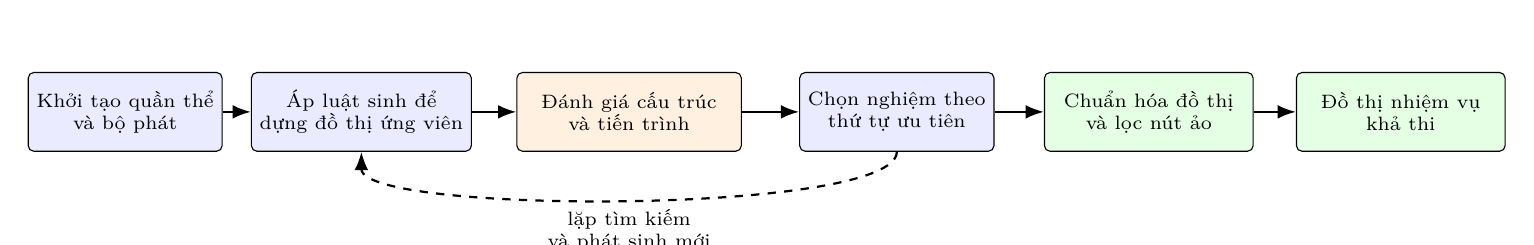
\begin{tikzpicture}[
  font=\scriptsize,
  >=Latex,
  flowbox/.style={draw, rounded corners=2pt, align=center, fill=blue!8, minimum width=2.45cm, minimum height=1.0cm, inner sep=3pt},
  evalbox/.style={draw, rounded corners=2pt, align=center, fill=orange!12, minimum width=2.85cm, minimum height=1.0cm, inner sep=3pt},
  resultbox/.style={draw, rounded corners=2pt, align=center, fill=green!10, minimum width=2.65cm, minimum height=1.0cm, inner sep=3pt},
  arr/.style={->, line width=0.8pt}
]
\node[flowbox] (s1) at (0,0) {Khởi tạo quần thể\\và bộ phát};
\node[flowbox] (s2) at (3.0,0) {Áp luật sinh để\\dựng đồ thị ứng viên};
\node[evalbox] (s3) at (6.4,0) {Đánh giá cấu trúc\\và tiến trình};
\node[flowbox] (s4) at (9.8,0) {Chọn nghiệm theo\\thứ tự ưu tiên};
\node[resultbox] (s5) at (13.0,0) {Chuẩn hóa đồ thị\\và lọc nút ảo};
\node[resultbox] (s6) at (16.2,0) {Đồ thị nhiệm vụ\\khả thi};
\draw[arr] (s1) -- (s2);
\draw[arr] (s2) -- (s3);
\draw[arr] (s3) -- (s4);
\draw[arr] (s4) -- (s5);
\draw[arr] (s5) -- (s6);
\draw[arr, dashed] (s4.south) .. controls +(0,-0.8) and +(0,-0.8) .. node[below, align=center] {lặp tìm kiếm\\và phát sinh mới} (s2.south);
\end{tikzpicture}
}
\caption{Luồng sinh đồ thị nhiệm vụ bằng tìm kiếm tiến hóa: khởi tạo cá thể, áp luật sinh, chấm điểm theo cấu trúc và tiến trình, chọn nghiệm khả thi ưu tiên cao rồi chuẩn hóa đồ thị đầu ra.}
\label{fig:mission_graph_generation_flow}
\end{figure}

\noindent Hình~\ref{fig:mission_graph_generation_flow} cho thấy nhánh tìm kiếm không dừng ở bước sinh cấu trúc thô. Một đồ thị chỉ được chuyển sang các khối hạ nguồn sau khi đã lần lượt trải qua dựng ứng viên, chấm điểm, chọn nghiệm theo thứ tự ưu tiên khả thi và loại nút ảo. Vì vậy, sơ đồ này đã bao quát đủ chuỗi vận hành thực tế của Khối~I, thay vì chỉ mô tả riêng lõi tiến hóa.

\subsubsection{Ưu tiên nghiệm khả thi và áp lực ràng buộc}
Để làm tường minh lớp sinh cấu trúc đồ thị nhiệm vụ, ta mô hình hóa mỗi cá thể bằng bộ ba: chuỗi luật (genome), đồ thị sinh ra (phenotype), và bộ chẩn đoán khả thi. Cụ thể:
\begin{equation}
g=(r_1,\ldots,r_L),\qquad
\mathcal{G}=\mathcal{T}(g),\qquad
(f,v,\phi)=\mathcal{E}(\mathcal{G}),
\end{equation}
trong đó $L$ là độ dài genome, $\mathcal{T}$ là thủ tục áp chuỗi luật để sinh đồ thị, $f\in[0,1]$ là fitness, $v\ge 0$ là tổng mức vi phạm ràng buộc, và $\phi=\mathbf{1}[v\le 10^{-9}]$ là cờ khả thi. Đại lượng $\mathcal{E}$ gộp độ khớp tension curve, bộ mô tả cấu trúc và các hạng vi phạm như độ dài đường chính, dải số nút/cạnh, realism, directionality, rejection ratio và cân bằng nhánh--vòng, đúng với quy trình chấm điểm đồ thị ở tầng hiện thực.

Trong bước chọn nghiệm, bộ sinh dùng thứ tự khả thi-ưu tiên kiểu Deb \cite{deb2000constraint}:
\begin{equation}
\kappa(i)=\big(\mathbf{1}[\neg\phi_i],\,(1-\phi_i)\,v_i,\,-f_i,\,\varepsilon_i\big),
\end{equation}
với $\varepsilon_i$ là lỗi realism của cấu trúc đồ thị. Cá thể có khóa từ điển nhỏ hơn sẽ được ưu tiên trong tournament và survivor selection, nên quần thể khả thi luôn được xếp trước quần thể không khả thi.

\begin{algorithm}[H]
\caption{Sinh đồ thị nhiệm vụ bằng GA hoặc CVT-emitter với ưu tiên nghiệm khả thi}
\label{alg:graph_evolution_feasible_first}
\begin{algorithmic}[1]
\Require Mục tiêu đường cong $\tau$, cấu hình $(P,G,L)$, chiến lược $s\in\{\text{GA},\text{CVT-emitter}\}$
\Ensure Đồ thị nhiệm vụ $\mathcal{G}^{\star}$
\If{$s=\text{CVT-emitter}$}
  \State $B \gets P\cdot G$ \Comment{ngân sách đánh giá}
  \State Khởi tạo kho lưu trữ CVT
  \For{$e=1$ đến $B$}
    \State Phát sinh một genome từ emitter (khởi tạo ngẫu nhiên hoặc dẫn hướng từ kho lưu trữ)
    \State Sinh đồ thị từ chuỗi luật hiện tại, rồi tính $(f,v,\phi)$ cho đồ thị đó
    \State Cập nhật kho lưu trữ và cá thể tốt nhất theo khóa $\kappa$
  \EndFor
\Else
  \State Khởi tạo quần thể ban đầu kích thước $P$
  \For{$t=1$ đến $G$}
    \State Đánh giá toàn bộ quần thể bằng thủ tục sinh đồ thị rồi chấm điểm ràng buộc
    \If{$\max f \ge 0.95$}
      \State \textbf{break} \Comment{dừng sớm khi đã hội tụ}
    \EndIf
    \State Sinh thế hệ con bằng tournament selection, lai ghép và đột biến thích nghi
    \State Đánh giá offspring
    \State Chọn cá thể sống sót theo quy tắc khả thi-ưu tiên trong mô hình $(\mu+\lambda)$
  \EndFor
\EndIf
\State Hậu xử lý đồ thị tốt nhất: sửa tiến trình, lọc virtual node, kiểm tra hợp lệ cấu trúc đồ thị
\State \Return $\mathcal{G}^{\star}$
\end{algorithmic}
\end{algorithm}

Thuật toán \ref{alg:graph_evolution_feasible_first} tóm tắt cách Khối I vận hành trong thực tế: mục tiêu chất lượng được tối ưu đồng thời với áp lực ràng buộc xuyên suốt từ lúc áp luật grammar, đánh giá cá thể, chọn sống sót cho đến hậu kiểm đầu ra.

Về mặt phương pháp, cách tổ chức này kế thừa trực tiếp tư duy của giải thuật di truyền, chiến lược tiến hóa và tối ưu ràng buộc theo ưu tiên nghiệm khả thi trong văn liệu tiến hóa cổ điển \cite{goldberg1989genetic,beyer2002evolution,deb2000constraint}.

\paragraph{Bất biến, điều kiện dừng và chi phí.}
Gọi $n=|V|$, $m=|E|$, $P$ là kích thước quần thể, $G$ là số thế hệ và $L$ là độ dài genome. Tính đúng của thủ tục tìm kiếm được duy trì bởi ba tầng kiểm soát nối tiếp nhau. Ở tầng sinh phenotype, các phép mở rộng bị chặn bởi trạng thái hiện hành nên không tạo ra hành động trái với ngữ nghĩa tiến trình. Ở tầng đánh giá, cờ khả thi $\phi=\mathbf{1}[v\le 10^{-9}]$ tách rõ nghiệm thỏa ràng buộc khỏi nghiệm còn vi phạm. Cuối cùng, trước khi chấp nhận đầu ra, đồ thị còn phải vượt qua hậu kiểm về liên thông, cặp start-goal, độ dài đường đi tối thiểu, quan hệ boss-goal và việc loại bỏ virtual node. Điều kiện dừng phụ thuộc vào chiến lược tìm kiếm: với GA, vòng lặp kết thúc khi đã xét đủ $G$ thế hệ hoặc khi độ thích nghi tốt nhất đạt ngưỡng hội tụ $0.95$; với CVT-emitter, quá trình dừng khi ngân sách $P\cdot G$ lần đánh giá đã được sử dụng hết. Dưới mô hình chi phí đã nêu, cận trên của độ phức tạp là:
\begin{equation}
\mathcal{O}\!\left(PG\,(C_{\text{exec}}+C_{\text{eval}})+PG\log P\right)
\end{equation}
cho nhánh GA, và
\begin{equation}
\mathcal{O}\!\left(PG\,(C_{\text{exec}}+C_{\text{eval}})\right)
\end{equation}
cho nhánh CVT-emitter.

\subsection{Khối mã hóa điều kiện từ đồ thị sang phòng (Khối III)}
Khối III ánh xạ ngữ cảnh đồ thị nhiệm vụ sang vector điều kiện cho từng phòng đích. Với phòng $i$, bộ điều kiện được xây từ hai nguồn: ngữ cảnh cục bộ và ngữ cảnh toàn cục.
\begin{align}
c_i^{\text{local}} &= f_{\text{local}}\big([z_{N}, z_{S}, z_{E}, z_{W}, b_i, p_i]\big),\\
H &= \mathrm{GNN}(G; X, E, \mathrm{TPE}), \quad c_i^{\text{global}} = H_i,\\
c_i &= \mathrm{Attn}(q=c_i^{\text{local}}, K=H, V=H) + f_{\text{fuse}}\big([c_i^{\text{local}}, c_i^{\text{global}}]\big).
\end{align}
Trong đó $z_{N,S,E,W}$ là latent của các phòng lân cận theo bốn hướng, $b_i$ là ràng buộc biên và $p_i$ là đặc trưng vị trí phòng. Nhánh toàn cục hỗ trợ nhiều biến thể GNN; cấu hình mặc định ưu tiên GPS cho bài toán đồ thị có tín hiệu toàn cục mạnh \cite{rampasek2022gps}. Ngoài ra, các thiên kiến cấu trúc theo kiểu Graphormer, như khoảng cách đường đi ngắn nhất và độ lệch cấu trúc theo quan hệ cạnh, cũng là cơ sở lý thuyết để củng cố lớp mã hóa đồ thị trong khối này \cite{ying2021graphormer}. Tầng attention đóng vai trò căn chỉnh thông tin toàn cục với ngữ cảnh cục bộ của từng phòng, từ đó giảm mâu thuẫn giữa ràng buộc biên và vai trò gameplay trong toàn bộ dungeon.

Về trực giác, cách đưa điều kiện vào đồng thời ở nhánh cục bộ và nhánh toàn cục cũng gần với dòng sinh có điều kiện theo ngữ nghĩa không gian, nơi thông tin điều kiện phải được giữ đúng vị trí và đúng vai trò thay vì chỉ bị nén thành một vector toàn cục \cite{park2019spade,hu2020graph2plan,inoue2023layoutdm}.

\begin{figure}[H]
\centering
\resizebox{0.96\linewidth}{!}{%
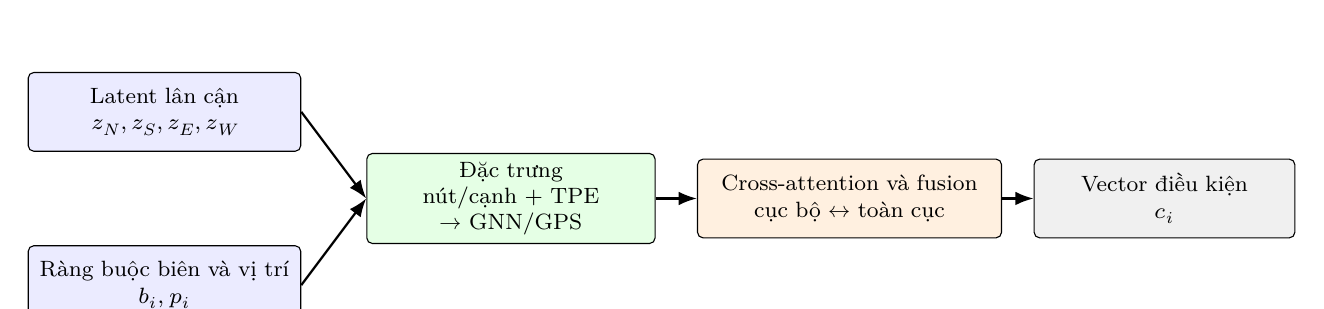
\begin{tikzpicture}[
  font=\footnotesize,
  >=Latex,
  lctx/.style={draw, rounded corners=2pt, fill=blue!8, align=center, text width=3.25cm, minimum height=1.0cm, inner sep=3pt},
  gctx/.style={draw, rounded corners=2pt, fill=green!10, align=center, text width=3.45cm, minimum height=1.0cm, inner sep=3pt},
  fusebox/.style={draw, rounded corners=2pt, fill=orange!12, align=center, text width=3.65cm, minimum height=1.0cm, inner sep=3pt},
  condbox/.style={draw, rounded corners=2pt, fill=gray!12, align=center, text width=3.1cm, minimum height=1.0cm, inner sep=3pt},
  arr/.style={->, line width=0.8pt}
]
\node[lctx] (l1) at (0,1.2) {Latent lân cận\\$z_N,z_S,z_E,z_W$};
\node[lctx] (l2) at (0,-1.0) {Ràng buộc biên và vị trí\\$b_i,p_i$};
\node[gctx] (g1) at (4.4,0.1) {Đặc trưng nút/cạnh + TPE\\$\rightarrow$ GNN/GPS};
\node[fusebox] (f1) at (8.7,0.1) {Cross-attention và fusion\\cục bộ $\leftrightarrow$ toàn cục};
\node[condbox] (o1) at (12.7,0.1) {Vector điều kiện\\$c_i$};
\draw[arr] (l1.east) -- (g1.west);
\draw[arr] (l2.east) -- (g1.west);
\draw[arr] (g1) -- (f1);
\draw[arr] (f1) -- (o1);
\end{tikzpicture}
}
\caption{Khối mã hóa điều kiện từ đồ thị sang phòng: hợp nhất ngữ cảnh cục bộ của phòng với ngữ cảnh toàn cục của đồ thị nhiệm vụ trước khi lấy mẫu.}
\label{fig:graph_to_room_conditioning}
\end{figure}

\subsection{Khối sinh nơ-ron: VQ-VAE (Khối II) và khuếch tán tiềm ẩn (Khối IV)}
Khối II đóng vai trò cầu nối giữa không gian tile rời rạc và không gian latent liên tục, còn Khối IV học quá trình khử nhiễu có điều kiện trên latent theo khung DDPM/DDIM \cite{ho2020ddpm,song2021ddim}. Ở pha suy luận, mô hình sử dụng classifier-free guidance (CFG), trong đó hệ số guidance $s_t$ thay đổi theo lịch chạy và được giữ trong miền đã hiệu chỉnh khi dùng bộ lấy mẫu nhanh \cite{ho2022cfg}. Vì miền này đã được hiệu chỉnh từ trước, nhánh lấy mẫu rút gọn không cho phép đẩy hệ số guidance vượt quá ngưỡng an toàn.

Ở bình diện tham chiếu rộng hơn, các họ mô hình như MaskGIT, consistency models và latent consistency models cho thấy hai hướng giảm số bước suy luận đang được quan tâm: tái cấu trúc bài toán sinh rời rạc theo cơ chế che khuất, hoặc học ánh xạ ít bước trong không gian liên tục \cite{chang2022maskgit,song2023consistency,luo2023lcm}. Chúng không phải là mô hình chính của khóa luận, nhưng là điểm tham chiếu phù hợp để đọc các nhánh suy luận rút gọn ở Chương 4.
\begin{equation}
\tilde{\epsilon}_{\theta}(x_t,t,c)=\epsilon_{\theta}(x_t,t,\varnothing)
+ s_t\Big(\epsilon_{\theta}(x_t,t,c)-\epsilon_{\theta}(x_t,t,\varnothing)\Big),
\end{equation}

Ở pha huấn luyện, diffusion loss được tái trọng số theo Min-SNR để giảm lệch trọng số giữa các timestep:
\begin{equation}
\mathrm{SNR}_t = \frac{\bar{\alpha}_t}{1-\bar{\alpha}_t}, \qquad
w_t = \frac{\min(\mathrm{SNR}_t,\gamma)}{\mathrm{SNR}_t+\varepsilon}, \qquad
\mathcal{L}_{\text{diff}} = \mathbb{E}_{t,\epsilon}\!\left[w_t\,\lVert \hat{y}_t - y_t\rVert_2^2\right],
\end{equation}

\begin{figure}[H]
\centering
\resizebox{0.94\linewidth}{!}{%
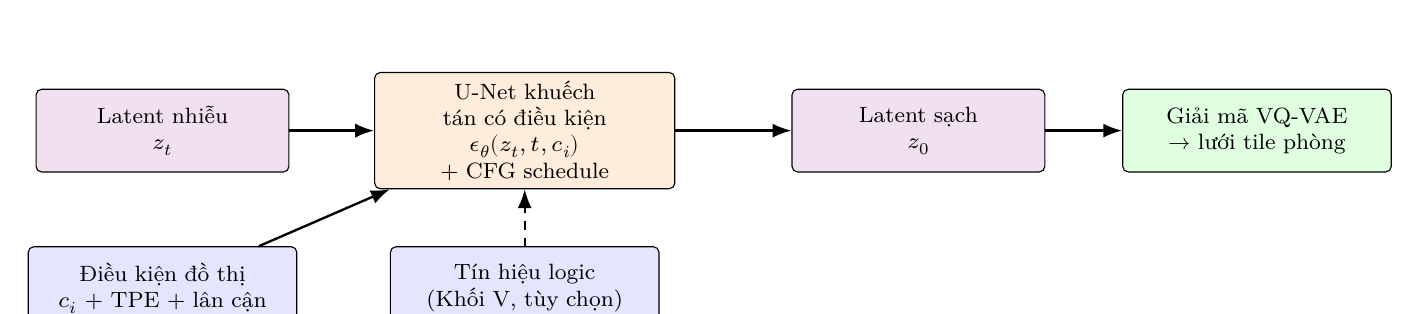
\begin{tikzpicture}[
  font=\footnotesize,
  >=Latex,
  latent/.style={draw, rounded corners=2pt, fill=violet!12, align=center, text width=3.0cm, minimum height=1.05cm, inner sep=3pt},
  cond/.style={draw, rounded corners=2pt, fill=blue!10, align=center, text width=3.2cm, minimum height=1.05cm, inner sep=3pt},
  diff/.style={draw, rounded corners=2pt, fill=orange!14, align=center, text width=3.6cm, minimum height=1.15cm, inner sep=3pt},
  outbox/.style={draw, rounded corners=2pt, fill=green!12, align=center, text width=3.2cm, minimum height=1.05cm, inner sep=3pt},
  arr/.style={->, line width=0.85pt}
]
\node[latent] (zt) at (0,0) {Latent nhiễu\\$z_t$};
\node[cond] (ci) at (0,-2.0) {Điều kiện đồ thị\\$c_i$ + TPE + lân cận};
\node[diff] (unet) at (4.6,0) {U-Net khuếch tán có điều kiện\\$\epsilon_\theta(z_t,t,c_i)$\\+ CFG schedule};
\node[latent] (z0) at (9.6,0) {Latent sạch\\$z_0$};
\node[outbox] (dec) at (13.9,0) {Giải mã VQ-VAE\\$\rightarrow$ lưới tile phòng};
\node[cond] (logic) at (4.6,-2.0) {Tín hiệu logic\\(Khối V, tùy chọn)};

\draw[arr] (zt) -- (unet);
\draw[arr] (ci) -- (unet);
\draw[arr, dashed] (logic) -- (unet);
\draw[arr] (unet) -- (z0);
\draw[arr] (z0) -- (dec);
\end{tikzpicture}
}
\caption{Sơ đồ khối khuếch tán tiềm ẩn (Khối IV) trong pha suy luận: latent nhiễu được khử nhiễu có điều kiện bằng U-Net + CFG, sau đó giải mã về lưới tile qua VQ-VAE.}
\label{fig:diffusion_model_detail}
\end{figure}
với $y_t$ là nhiễu mục tiêu (hoặc vận tốc $v$ khi bật v-prediction) và $\gamma$ là ngưỡng Min-SNR \cite{hang2023minsnr}.

\subsection{Khối hướng dẫn logic và sửa lỗi ký hiệu (Khối V--VI)}
Khối V bổ sung tín hiệu logic vào huấn luyện theo lộ trình tăng dần trọng số (\emph{warmup}) nhằm tránh gây nhiễu khi mô hình chưa ổn định:
\begin{equation}
\mathcal{L}_{\text{total}} = \alpha_{\text{visual}}\mathcal{L}_{\text{diff}} +
\mathbf{1}[e \ge e_{\text{warmup}}] \, \alpha_{\text{logic}}\mathcal{L}_{\text{logic}} +
\lambda_{\text{stage}}\mathcal{L}_{\text{stage}}.
\end{equation}
Ở nhánh tăng cường cho puzzle nhiều bước, $\lambda_{\text{stage}}$ là trọng số của
hạng mất mát mô tả ngữ nghĩa các giai đoạn puzzle. Hạng tử này chỉ hoạt động
khi mini-batch hiện tại thật sự mang đầy đủ thông tin về giai đoạn puzzle và
cấu hình huấn luyện bật chế độ giám sát tương ứng; nếu không,
$\lambda_{\text{stage}}=0$. Trong cấu hình hiện tại, nhánh dự đoán phụ được đặt
trên biểu diễn sau giải mã và học đồng thời bốn thuộc tính: họ cổng
(\emph{gate family}), cờ \emph{sequence-required}, số giai đoạn hữu hiệu, và
chuỗi giai đoạn có thứ tự. Viết gọn:
\begin{equation}
\mathcal{L}_{\text{stage}} =
\mathcal{L}_{\text{gate}} +
\mathcal{L}_{\text{seq}} +
\mathcal{L}_{\text{count}} +
\mathcal{L}_{\text{slot}},
\end{equation}
trong đó $\mathcal{L}_{\text{slot}}$ chỉ được cộng trên các vị trí stage hợp lệ
thực sự tồn tại trong chuỗi mục tiêu. Cấu trúc này buộc nhánh diffusion không
chỉ tiếp nhận thông tin giai đoạn ở đầu vào, mà còn phải tái hiện đúng ngữ
nghĩa tiến trình đó ngay ở đầu ra dự đoán của phòng.

Trong suy luận theo kiểu DDIM, tín hiệu hướng dẫn logic tác động trực tiếp lên
dự đoán nhiễu:
\begin{equation}
\hat{\epsilon}^{\,'}_\theta = \hat{\epsilon}_\theta + \sqrt{1-\bar{\alpha}_t}\,\nabla_{x_t}\mathcal{L}_{\text{logic}},
\end{equation}
rồi mới cập nhật lại $\hat{x}_0$. Cách viết này phản ánh đúng thao tác trong Khối IV khi logic guidance được bật.

Sau giải mã, Khối VI xử lý phòng theo chuỗi chuẩn hóa gồm làm sạch dữ liệu, ép biên và sửa cục bộ có điều kiện theo mặt nạ kế hoạch. Thành phần inpainting có dẫn dắt bởi WFC được dùng như một bước sửa cục bộ khi phát hiện vùng vi phạm ràng buộc \cite{karth2021wfc}. Vì mặt nạ kế hoạch được suy ra từ ngữ nghĩa đồ thị (vai trò phòng, cửa bắt buộc, quan hệ vào/ra), bước sửa lỗi không chỉ cải thiện hình học mà còn phục hồi tính đúng của tiến trình gameplay.

Mục tiêu của thuật toán là giữ nhất quán giữa tầng nơ-ron và tầng ký hiệu: đầu vào là lưới nơ-ron cùng ngữ cảnh đồ thị phòng, đầu ra là lưới đã chuẩn hóa ngữ nghĩa, thỏa ràng buộc biên-cửa và bảo toàn khả giải cục bộ. Trình tự xử lý được cố định theo chuỗi chuẩn hóa $\rightarrow$ ép biên $\rightarrow$ sửa có phản hồi theo mặt nạ kế hoạch $\rightarrow$ phủ marker đồ thị $\rightarrow$ kiểm tra hợp lệ, nhờ đó mọi thay đổi đều có thể truy vết và kiểm chứng.

\begin{algorithm}[H]
\caption{Sửa phòng có phản hồi ký hiệu ở tầng hậu xử lý}
\label{alg:room_repair_feedback}
\begin{algorithmic}[1]
\Require Lưới nơ-ron đầu vào $x_i^{\text{neural}}$, đồ thị phòng $G_i$, cặp start-goal $(s_i,g_i)$
\Ensure Lưới cuối $x_i^{\text{final}}$ thỏa ràng buộc biên và đường đi
\State $x_i^{\text{final}} \gets$ Chuẩn hóa mã ngữ nghĩa của $x_i^{\text{neural}}$ về từ điển tile hợp lệ
\State $x_i^{\text{final}} \gets$ Loại bỏ các marker biến động không cần duy trì ở đầu ra phòng
\State $x_i^{\text{final}} \gets$ Khôi phục vỏ biên theo ràng buộc cửa-biên của $G_i$
\State $m_i \gets$ Dựng dấu vết kế hoạch từ $G_i$ và cặp $(s_i,g_i)$
\If{bước sửa hậu kỳ được kích hoạt}
  \State $x_i^{\text{cand}} \gets$ Sinh ứng viên sửa có phản hồi ký hiệu từ $x_i^{\text{final}}$ và $m_i$
  \If{bước sửa tạo ra cấu hình hợp lệ}
    \State $x_i^{\text{final}} \gets x_i^{\text{cand}}$
  \EndIf
\EndIf
\State $x_i^{\text{final}} \gets$ Chồng các marker tiến trình từ đồ thị lên lưới đã sửa
\State Kiểm tra lại kích thước phòng và tính hợp lệ hình học của $x_i^{\text{final}}$
\State \Return $x_i^{\text{final}}$
\end{algorithmic}
\end{algorithm}

Thuật toán \ref{alg:room_repair_feedback} là lớp nối giữa chất lượng hình học và tính đúng gameplay. Nếu thiếu lớp này, các sai lệch cục bộ về cửa, biên hoặc đường đi có thể lan sang bước ghép dungeon và làm giảm độ tin cậy của đánh giá toàn cục.

\paragraph{Điều kiện hợp lệ và chi phí hậu xử lý.}
Ở tầng hậu xử lý, một phòng chỉ được xem là hợp lệ khi đồng thời bảo toàn kích thước chuẩn, duy trì đúng quan hệ biên-cửa do ngữ cảnh đồ thị áp đặt, và không làm suy giảm khả giải cục bộ sau bước sửa cùng thao tác phủ lại marker tiến trình. Điều kiện dừng là hiển nhiên vì chuỗi chuẩn hóa luôn hữu hạn, còn nhánh sửa lặp được chặn trên bởi số lần thử tối đa do cấu hình thực thi quy định. Bởi vậy, độ phức tạp theo phòng là:
\begin{equation}
\mathcal{O}\!\left(HW + R\,C_{\text{rep}}(H,W)\right),
\end{equation}
với $R$ là số vòng repair thực thi.

\paragraph{Ngữ pháp puzzle trạng thái nhiều bước ở tầng hậu xử lý.}
Phiên bản hiện tại của Khối VI không còn xem phòng puzzle chỉ như một biến thể
hình học có gắn thêm vài marker ngữ nghĩa. Thay vào đó, mỗi phòng có trạng thái
được gắn với một kế hoạch puzzle hữu hạn, mô tả tuần tự các hành động bắt buộc
như thu thập chìa khóa, lấy vật phẩm, kích hoạt cơ cấu puzzle hoặc đẩy khối vào
công tắc. Chuỗi giai đoạn này được suy ra từ ngữ nghĩa cạnh và vai trò của
phòng trong đồ thị nhiệm vụ, rồi được chuẩn hóa thành siêu dữ liệu dùng chung cho
khâu sinh và khâu thẩm định. Vì thế, một cửa phụ thuộc puzzle không còn được
hiểu như chi tiết trang trí cục bộ, mà như một điều kiện tiến trình chỉ mở khi
chuỗi giai đoạn tương ứng đã được hoàn tất trong trạng thái chơi. Cách tổ chức
này chuyển hệ thống từ việc bố trí biểu tượng puzzle trên bề mặt phòng sang mô
hình hóa puzzle như một tiến trình trạng thái có thể kiểm chứng; tầng ngữ pháp
và tầng xác nhận giữ trách nhiệm về tính đúng, còn mô hình nơ-ron tập trung vào
hình học và bề mặt thị giác.

Trong biến thể tăng cường gần nhất, cùng siêu dữ liệu giai đoạn này còn được dùng ở
pha huấn luyện như một tín hiệu giám sát tường minh. Thay vì chỉ điều kiện hóa
mô hình bằng thông tin giai đoạn, biến thể này bổ sung một nhánh dự đoán phụ để
buộc phân bố sau giải mã bảo toàn đúng họ cổng, yêu cầu tuần tự, số giai đoạn
hữu hiệu và trật tự xuất hiện của chúng. Nhờ vậy, nhận định rằng mô hình học
được ngữ nghĩa puzzle nhiều bước không còn chỉ dựa vào ngữ pháp lai ở thời điểm
suy luận, mà được hỗ trợ ngay từ mục tiêu tối ưu trong huấn luyện. Dù vậy, các
mô hình đã huấn luyện trước đó chưa chứa hạng mất mát bổ sung này không được sử
dụng như bằng chứng cho kết luận trên.

\subsection{Khối hậu kiểm: bộ kiểm tra cơ học, P-CBS và bước chuẩn hóa trước thẩm định (Khối VII)}
Khối VII khép lại đường sinh của hệ thống sau khi các phòng riêng lẻ đã được
ghép thành một dungeon hoàn chỉnh. Thay vì giao toàn bộ việc đánh giá cho một
bộ giải duy nhất, khóa luận tách rõ hai tầng xác nhận với hai câu hỏi khác nhau:
tầng thứ nhất quyết định dungeon có đúng cơ học hay không, còn tầng thứ hai đo
mức ma sát nhận thức mà từng persona gặp phải khi tương tác với cùng đầu ra đó.
Cách tách này phù hợp với thực hành kiểm thử tự động: các persona thủ tục cổ
điển chủ yếu dùng MCTS hoặc RL để mô phỏng lối chơi, trong khi các
bộ giải trạng thái tối ưu được dùng để kiểm tra tính beatable/solvable về mặt
cơ học \cite{holmgard2016personasclones,holmgard2018proceduralpersonas,ariyurek2023beyondpersonas}. Trong phạm vi khóa luận này, tầng kiểm tra cơ học
gồm ba phép kiểm nối tiếp: kiểm tra khả đi ở mức phòng có tham chiếu đồ thị,
kiểm tra tiến trình trên đồ thị, và phát hiện soft-lock mang tính quyết định.
Phép kiểm A* toàn cục trên lưới ghép vẫn được
giữ như một phép thử áp lực bổ sung, bởi với các puzzle nhiều trạng thái nó
thường chạm giới hạn thời gian trước khi phủ hết không gian trạng thái.

\paragraph{Bước chuẩn hóa lưới ghép trước thẩm định.}
Để bảo đảm tầng thẩm định nhận đúng miền dữ liệu mà chương này mô tả, lưới ghép
không được chuyển thẳng sang bộ kiểm tra mà phải đi qua một bước chuẩn hóa bàn
giao. Bước này gồm bốn phép biến đổi hữu hạn: đưa đầu vào về ma trận số nguyên
hai chiều, ánh xạ mọi ký hiệu ngoài bộ từ vựng ngữ nghĩa về tile hợp lệ, lấp
các vùng \texttt{VOID} kín không thông ra biên ngoài, và chuẩn hóa duy nhất một
cặp \texttt{START}/\texttt{TRIFORCE}. Viết gọn:
\begin{equation}
D^{\star}=\Pi_{\mathrm{valid}}\!\left(D\right),
\end{equation}
trong đó $\Pi_{\mathrm{valid}}$ là phép chiếu từ lưới ghép thô sang miền hợp lệ
của bộ từ vựng tile và ràng buộc terminal. Bước chuẩn hóa này loại trừ ngay từ đầu
những sai lệch đầu vào có thể làm méo phán quyết thẩm định, đặc biệt là trường
hợp vùng rỗng bị giữ kín trong nội bộ lưới hoặc xuất hiện ký hiệu ngữ nghĩa nằm
ngoài từ điển chuẩn.

\paragraph{Bộ kiểm tra cơ học cho tính đúng.}
Sau chuẩn hóa, bộ kiểm tra cơ học chỉ công nhận dungeon là hợp lệ khi đồng thời thỏa ba điều kiện:
\begin{equation}
\phi_{\mathrm{hard}}(D^{\star})=
\mathbf{1}\!\left[
\phi_{\mathrm{guided}}(G,D^{\star}) \land
\phi_{\mathrm{prog}}(G,D^{\star}) \land
\phi_{\mathrm{softlock}}(D^{\star})
\right].
\end{equation}
Ở đây $\phi_{\mathrm{guided}}$ kiểm tra rằng đường tiến trình khả thi trong đồ
thị nhiệm vụ thật sự đi qua các phòng đã ghép và vẫn còn khả năng đi qua ở mức
phòng; $\phi_{\mathrm{prog}}$ kiểm tra tiến trình khóa--cổng--vật phẩm theo đồ
thị nhiệm vụ; còn $\phi_{\mathrm{softlock}}$ loại các trường hợp tồn tại ngõ
cụt không hồi phục. Phép kiểm A* nguyên khối trên lưới ghép vẫn được ghi nhận
riêng như một kiểm tra nghiêm ngặt hơn, nhưng không còn là cổng quyết định duy
nhất của báo cáo. Cách tổ chức này phản ánh đúng kiến trúc lấy đồ thị nhiệm vụ
làm trục chính hiện tại và tránh đánh đồng việc A* vượt ngưỡng thời gian trên
lưới ghép với việc dungeon
thật sự không chơi được.

\paragraph{P-CBS như bộ thẩm định hành vi giới hạn nhận thức.}
P-CBS (\emph{Persona-Driven Cognitive Bounded Search}) không được dùng như một bộ giải tối ưu tổng quát, mà như một bộ thẩm định theo persona đặt sau bộ kiểm tra cơ học để trả lời câu hỏi cụ thể hơn: ``một người chơi kiểu này có tìm ra lời giải trong giới hạn chú ý, trí nhớ làm việc và ngân sách cân nhắc hay không?'' Khác với persona thủ tục kiểu MCTS hoặc các mô hình đường đi chỉ mô phỏng định tính hiện tượng quên và lạc hướng \cite{holmgard2018proceduralpersonas,ariyurek2023beyondpersonas,rahmani2022humanlikepath,dubey2022cognitivepath}, P-CBS tìm kiếm trên không gian trạng thái tăng cường. Mỗi nút tìm kiếm lưu đồng thời vị trí hiện tại, trạng thái vật phẩm/tiến trình, các mốc tương tác (affordance) đã quan sát, dấu vết quay lại gần đây và phần ngân sách nhận thức còn lại.

Một lượt P-CBS trong khóa luận được hiểu theo bốn bước tuần tự:
\begin{enumerate}[label=\arabic*.]
  \item Chuẩn hóa dungeon đã vượt qua bộ kiểm tra cơ học và dựng tập hành động hợp lệ theo luật chơi hiện hành.
  \item Mở rộng các trạng thái ứng viên, trong đó mỗi trạng thái mang thêm bộ nhớ làm việc, các mốc tương tác đã thấy và số lần quay lại gần đây.
  \item Chấm điểm các hành động hợp lệ bằng hàm tiện ích phụ thuộc persona rồi ưu tiên mở rộng các hành động có giá trị cao hơn.
  \item Kết thúc khi persona đạt đích trong ngân sách cho phép, hoặc thất bại khi biên tìm kiếm cạn kiệt, ngân sách nhận thức hết, hay các mốc tương tác quan trọng không còn được khôi phục đủ tin cậy.
\end{enumerate}
Với một hành động $a$, hàm tiện ích dùng để xếp hạng nút kế là:
\begin{equation}
\begin{aligned}
U(a)=\;&\alpha \,\Delta g+\beta \,\mathrm{info\_gain}
-\gamma \,\mathrm{risk}
-\rho \,\mathrm{revisit} \\
&-\psi \,\mathrm{complexity}
-\omega \,\mathrm{conditional\_uncertainty}
+\eta \,\mathrm{frontier} \\
&+\xi \,\mathrm{affordance\_resume}
-\zeta \,\mathrm{affordance\_forgetting}.
\end{aligned}
\end{equation}
\begin{table}[H]
\centering
\small
\caption{Ý nghĩa các thành phần chính trong hàm tiện ích của P-CBS}
\label{tab:pcbs_term_meanings}
\begin{tabular}{>{\raggedright\arraybackslash}p{3.35cm} >{\raggedright\arraybackslash}p{8.45cm}}
\toprule
Thành phần & Ý nghĩa trực tiếp trong thẩm định \\
\midrule
$\Delta g$ & Mức tiến triển về mục tiêu hoặc mốc tiến trình chính; cao hơn nghĩa là hành động đưa persona gần đích hơn. \\
\texttt{info\_gain} & Lượng thông tin mới persona thu được sau một bước, ví dụ phát hiện phòng chức năng, mốc tương tác hoặc đường tắt. \\
\texttt{risk} & Rủi ro cục bộ khi bước vào trạng thái mới, như giao tranh, ngõ cụt hoặc vùng có hậu quả bất lợi. \\
\texttt{revisit} & Mức phạt cho quay lại vùng đã đi qua; thành phần này mô hình hóa sự mệt mỏi và giới hạn trí nhớ làm việc khi persona phải dò đường lại. \\
\texttt{complexity} & Độ phức tạp cục bộ của vùng kế tiếp, phản ánh số quyết định và mật độ vật cản/cổng điều kiện mà persona phải cân nhắc. \\
\shortstack[l]{\texttt{conditional\_}\\\texttt{uncertainty}} & Mức bất định khi đối mặt cửa khóa, cổng phá được hoặc dấu mốc câu đố mà trạng thái vật phẩm và niềm tin hiện tại chưa đủ mạnh để giải thích chắc chắn. \\
\texttt{frontier} & Phần thưởng cho việc mở rộng vùng biên chưa khám phá, giúp persona tiếp tục khám phá thay vì mắc kẹt quanh vùng quen thuộc. \\
\shortstack[l]{\texttt{affordance\_}\\\texttt{resume}} & Phần thưởng khi persona nhớ lại đúng một mốc tương tác đã quan sát trước đó sau khi trạng thái vật phẩm thay đổi. \\
\shortstack[l]{\texttt{affordance\_}\\\texttt{forgetting}} & Mức phạt khi persona lẽ ra có thể nối lại một mốc tương tác cũ nhưng bộ nhớ làm việc không còn giữ được liên hệ đó. \\
\bottomrule
\end{tabular}
\end{table}
Hai cơ chế làm nên khác biệt rõ nhất của P-CBS là $\mathrm{revisit}$ và $\mathrm{conditional\_uncertainty}$. Thành phần thứ nhất phạt việc quay lại các ô đã đi qua trong bối cảnh trí nhớ hữu hạn; thành phần thứ hai phạt việc lao vào các cấu trúc có điều kiện khi bằng chứng cục bộ và trạng thái vật phẩm chưa đủ mạnh. Cách mô hình hóa này gần với khung lập kế hoạch hữu hạn tài nguyên ở mức ý tưởng \cite{callaway2022cognitiveresources,lancia2023inforl}, nhưng được hiện thực trực tiếp ở tầng quyết định mở rộng nút của bộ giải dungeon thay vì ở tầng chính sách học sâu hay suy luận siêu mức.

Trong phiên bản cuối của P-CBS, hai số hạng $\xi$ và $\zeta$ mô hình hóa \emph{bộ nhớ affordance tiến trình}: tác tử có thể nhớ lại một cửa khóa, một cổng phá được bằng bom hay một mốc câu đố đã quan sát trước đó sau khi trạng thái vật phẩm thay đổi, đồng thời vẫn bị phạt nếu mốc tương tác đó không còn được bộ nhớ làm việc hỗ trợ tốt. Vì vậy, P-CBS phù hợp để phát hiện các trường hợp ``dungeon vẫn có lời giải nhưng persona chưa nối lại được lời giải ấy'' -- đúng kiểu sai khác mà bộ kiểm tra cơ học không đo được.

\paragraph{Persona và chỉ số nhận thức.}
P-CBS cho phép thay trọng số theo persona mà không phải thay đổi đầu vào của bộ thẩm định. Trong hiện thực mã nguồn, hệ thống hỗ trợ nhiều hồ sơ hành vi; tuy nhiên, để giữ cách đọc nhất quán trong khóa luận, ba hồ sơ chuẩn hóa được dùng làm mốc diễn giải là \emph{novice}, \emph{balanced} và \emph{speedrunner}. Bảng~\ref{tab:pcbs_persona_profiles} tóm tắt trực tiếp các khác biệt cốt lõi giữa ba hồ sơ này ở mức trí nhớ, thiên hướng tiến đích và mức phạt bất định. Theo đó, \emph{speedrunner} ưu tiên tiến độ và duy trì bộ nhớ mạnh hơn, trong khi \emph{novice} chịu phạt cao hơn trước nguy cơ chiến đấu, độ phức tạp và bất định có điều kiện.

\begin{table}[H]
\centering
\small
\caption{Ba hồ sơ persona chuẩn hóa dùng để diễn giải P-CBS trong khóa luận}
\label{tab:pcbs_persona_profiles}
\begin{tabular}{>{\raggedright\arraybackslash}p{2.2cm}cccc>{\raggedright\arraybackslash}p{5.2cm}}
\toprule
Persona & $m$ & $\alpha$ & $\rho$ & $\omega$ & Diễn giải ngắn \\
\midrule
\emph{Novice} & 5 & 0.35 & 0.10 & 0.60 & Tầm nhìn hẹp hơn, trí nhớ làm việc thấp hơn và bị phạt mạnh bởi nguy cơ, quay lui, độ phức tạp và bất định có điều kiện. \\
\emph{Balanced} & 7 & 0.58 & 0.06 & 0.05 & Hồ sơ trung tâm dùng cho các bảng định lượng chính; cân bằng giữa tiến đích, khám phá và kiểm soát rủi ro. \\
\emph{Speedrunner} & 10 & 0.80 & 0.55 & 0.05 & Bộ nhớ mạnh, thiên hướng tiến đích cao và chấp nhận rủi ro nhiều hơn để rút ngắn quãng đường đến mục tiêu. \\
\bottomrule
\end{tabular}
\end{table}

Trong Bảng~\ref{tab:pcbs_persona_profiles}, $m$ là dung lượng trí nhớ làm việc của persona, $\alpha$ là trọng số tiến đích trong hàm tiện ích, $\rho$ là mức phạt cho quay lui, còn $\omega$ là mức phạt do bất định có điều kiện. Từ quỹ đạo tìm kiếm thu được, hệ thống trích xuất các chỉ số hành vi như entropy điều hướng, tổng số lần quay lại và \emph{goal-sighting latency} (độ trễ nhận thức mục tiêu: số bước kể từ khi persona lần đầu tiên quan sát được mục tiêu hoặc affordance quan trọng cho đến khi thật sự đạt được, phản ánh hiệu quả khai thác thông tin):
\begin{equation}
H_{\mathrm{nav}}=-\sum_{v\in \mathcal{V}_{\mathrm{path}}} p(v)\log_2 p(v),
\qquad
\mathrm{CGR}=
\frac{\sum_{j=1}^{M}\mathbf{1}\!\left[\phi_{\mathrm{hard}}(D_j^{\star})=1 \land \phi_{\mathrm{pcbs}}(D_j^{\star})=0\right]}
{\sum_{j=1}^{M}\mathbf{1}\!\left[\phi_{\mathrm{hard}}(D_j^{\star})=1\right]},
\end{equation}
trong đó $H_{\mathrm{nav}}$ là entropy điều hướng còn $\mathrm{CGR}$ đo phần trăm trường hợp lệch giữa ``giải được về cơ học'' và ``điều hướng được với persona''. Với thiết kế này, Chương 4 có thể đọc riêng hai câu hỏi: dungeon có đúng cơ học hay không, và nếu đúng cơ học thì persona nào vẫn bị lạc, do dự hoặc chậm ở các vùng puzzle.

\begin{figure}[H]
\centering
\resizebox{0.92\linewidth}{!}{%
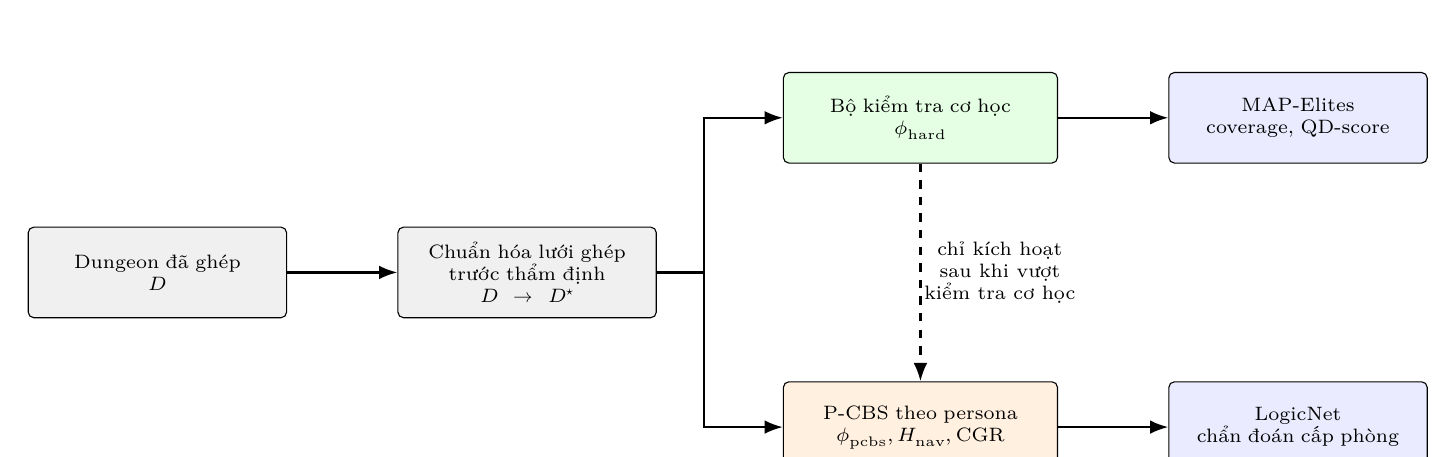
\begin{tikzpicture}[
  font=\scriptsize,
  >=Latex,
  node distance=12mm and 14mm,
  valbox/.style={draw, rounded corners=2pt, fill=gray!12, align=center, text width=3.0cm, minimum height=1.15cm, inner sep=4pt},
  mechbox/.style={draw, rounded corners=2pt, fill=green!10, align=center, text width=3.2cm, minimum height=1.15cm, inner sep=4pt},
  cogbox/.style={draw, rounded corners=2pt, fill=orange!12, align=center, text width=3.2cm, minimum height=1.15cm, inner sep=4pt},
  qdbox/.style={draw, rounded corners=2pt, fill=blue!8, align=center, text width=3.0cm, minimum height=1.15cm, inner sep=4pt},
  arr/.style={->, line width=0.8pt}
]
\node[valbox] (d0) {Dungeon đã ghép\\$D$};
\node[valbox, right=of d0] (d1) {Chuẩn hóa lưới ghép\\trước thẩm định\\$D \rightarrow D^\star$};
\node[mechbox, above right=8mm and 16mm of d1] (d2) {Bộ kiểm tra cơ học\\$\phi_{\mathrm{hard}}$};
\node[cogbox, below right=8mm and 16mm of d1] (d3) {P-CBS theo persona\\$\phi_{\mathrm{pcbs}}, H_{\mathrm{nav}}, \mathrm{CGR}$};
\node[qdbox, right=of d2] (d4) {MAP-Elites\\coverage, QD-score};
\node[qdbox, right=of d3] (d5) {LogicNet\\chẩn đoán cấp phòng};
\draw[arr] (d0) -- (d1);
\draw[arr] (d1.east) -- ++(0.6,0) |- (d2.west);
\draw[arr] (d1.east) -- ++(0.6,0) |- (d3.west);
\draw[arr] (d2) -- (d4);
\draw[arr] (d3) -- (d5);
\draw[arr, dashed] (d2.south) -- node[midway, right, align=center, fill=white, inner sep=1pt] {chỉ kích hoạt\\sau khi vượt\\kiểm tra cơ học} (d3.north);
\end{tikzpicture}%
}
\caption{Tầng hậu sinh sau khi ghép dungeon: chuẩn hóa lưới ghép, kiểm tra cơ học, thẩm định P-CBS theo persona và hai nhánh đánh giá bổ trợ ở mức phòng và mức kho lưu trữ.}
\label{fig:post_generation_validation_stack}
\end{figure}

Trong đường chạy hậu sinh, bước chuẩn hóa lưới ghép không chỉ là một thao tác tiền xử lý kỹ thuật mà còn là điểm tách trách nhiệm giữa bộ sinh và bộ thẩm định. Các thống kê như số tile ngoài từ điển, số vùng \texttt{VOID} kín phải lấp và số terminal trùng bị loại được lưu riêng trong $\mathcal{I}_{\mathrm{handoff}}$; đồng thời P-CBS chỉ được kích hoạt sau khi bộ kiểm tra cơ học xác nhận dungeon hợp lệ về mặt luật chơi, nhờ đó các chỉ số nhận thức không bị nhiễu bởi lỗi miền biểu diễn.

\section{Thuật toán huấn luyện, suy luận và hậu kiểm}

\subsection{Huấn luyện theo giai đoạn}
Huấn luyện được tổ chức theo chuỗi VQ-VAE $\rightarrow$ diffusion $\rightarrow$ nhánh lấy mẫu nhanh $\rightarrow$ nhánh che khuất, trong đó mỗi giai đoạn có checkpoint riêng để phục vụ tiếp tục huấn luyện và phân tích loại trừ. Ở giai đoạn diffusion, mỗi batch lần lượt được mã hóa từ phòng thật sang latent tương ứng, dựng điều kiện từ đồ thị sang phòng đúng lược đồ, tính \(\mathcal{L}_{\text{diff}}\) với trọng số Min-SNR, rồi mới cộng hạng mất mát logic theo lịch warmup. Các bước an toàn như bỏ qua batch không hữu hạn, cắt gradient và EMA được duy trì trong vòng lặp chính để hạn chế lỗi tối ưu hóa lan truyền theo thời gian huấn luyện.

Ở mức hiện thực, bộ lập lịch và điểm kiểm tra theo giai đoạn giữ vai trò neo để chuyển pha huấn luyện mà không làm đứt mạch tối ưu hóa. Khi kết hợp với kiểm tra không hữu hạn, cắt gradient và EMA, vòng lặp huấn luyện giữ được cả độ ổn định số học lẫn khả năng truy vết khi tiếp tục thí nghiệm.

Để mã giả có tính học thuật và dễ đối chiếu, khóa luận theo quy ước trình bày thường gặp trong các bài báo gốc về diffusion và graph diffusion: tách rõ nhánh train/sampling, nêu tường minh input-output, và đặt tên bước theo hành động thuật toán ở mức trừu tượng (ví dụ: lấy mẫu, gom batch, cập nhật) thay vì dùng trực tiếp tên hàm triển khai trong mã nguồn \cite{ho2020ddpm,song2021ddim,vignac2023digress,mouret2015mapelites}.

\begin{algorithm}[H]
\caption{Huấn luyện một epoch diffusion với warmup logic}
\label{alg:train_epoch_diffusion}
\begin{algorithmic}[1]
\Require Dataloader $\mathcal{D}$ trả về $(x,\mathcal{G})$, cấu hình huấn luyện
\Ensure Tham số diffusion/condition encoder được cập nhật ổn định
\State $\mathbb{I}_{\text{logic}} \gets \mathbf{1}\!\left[\textit{epoch} \ge e_{\text{warmup}}\right]$
\ForAll{$(x,\mathcal{G}) \in \mathcal{D}$}
  \State Mã hóa từng đồ thị trong $\mathcal{G}$ thành vector điều kiện $c_i$
  \State Gom các vector điều kiện thành lô $C_{\text{batch}}$
  \State Gom các đồ thị thành lô $G_{\text{batch}}$
  \State Tính $\mathcal{L}_{\text{diff}}$ với trọng số Min-SNR
  \If{$\mathbb{I}_{\text{logic}}=1$}
    \State Tính $\mathcal{L}_{\text{logic}}$ trên latent dự đoán
  \Else
    \State $\mathcal{L}_{\text{logic}} \gets 0$
  \EndIf
  \If{giám sát ngữ nghĩa cho puzzle stage được bật}
    \State Giải mã đầu ra dự đoán ở cấp phòng và tính $\mathcal{L}_{\text{stage}}$
  \Else
    \State $\mathcal{L}_{\text{stage}} \gets 0$
  \EndIf
  \State $\mathcal{L}_{\text{total}} \gets \alpha_{\text{visual}}\mathcal{L}_{\text{diff}} + \alpha_{\text{logic}}\mathcal{L}_{\text{logic}} + \lambda_{\text{stage}}\mathcal{L}_{\text{stage}}$
  \If{$\mathcal{L}_{\text{total}}$ hoặc gradient không hữu hạn}
    \State Bỏ qua batch hiện tại, tăng bộ đếm mất ổn định và chuyển sang batch kế tiếp
  \EndIf
  \State Thực hiện một bước tối ưu, cắt gradient và cập nhật EMA
\EndFor
\State Cập nhật bộ lập lịch và nhiệt độ LogicNet theo bước toàn cục
\end{algorithmic}
\end{algorithm}

Theo nghĩa phương pháp luận, Thuật toán \ref{alg:train_epoch_diffusion} hiện thực
trực tiếp nguyên tắc ổn định trước, ràng buộc sau: tín hiệu logic được đưa vào
có kiểm soát để tránh làm lệch gradient ở giai đoạn mô hình chưa hội tụ đủ.

Ở mức triển khai, hai bước gom lô điều kiện và gom lô đồ thị được tổ chức thành
hai thủ tục đóng gói tensor riêng nhưng cùng tuân theo quy ước dữ liệu đã mô
tả ở trên.

\paragraph{Bất biến tối ưu hóa và độ phức tạp.}
Ở bước cập nhật tham số, tính đúng của vòng lặp huấn luyện không được hiểu là
tạo ra đầu ra cuối cùng hợp lệ, mà là duy trì đầy đủ các bất biến cần thiết để
quá trình tối ưu diễn ra ổn định. Cụ thể, mỗi mini-batch phải thỏa bốn điều
kiện: giá trị mất mát và gradient luôn hữu hạn; tensor điều kiện từ đồ thị sang phòng
đúng lược đồ dữ liệu đã đặc tả; thành phần $\mathcal{L}_{\text{logic}}$ chỉ
được kích hoạt sau ngưỡng warmup $e_{\text{warmup}}$; và thành phần
$\mathcal{L}_{\text{stage}}$ chỉ được cộng khi batch có metadata stage hợp lệ.
Một epoch kết thúc tự nhiên sau khi dataloader được duyệt hết, tương đương
$|\mathcal{D}|$ bước cập nhật. Do đó, với mô hình chi phí theo batch, độ phức
tạp xấp xỉ:
\begin{equation}
\mathcal{O}\!\left(|\mathcal{D}|\cdot\left(C_{\text{enc}} + C_{\text{diff}} + \mathbb{I}_{\text{logic}}C_{\text{logic}} + \mathbb{I}_{\text{stage}}C_{\text{stage}}\right)\right),
\end{equation}
trong đó $C_{\text{diff}}$ là hạng chi phối.

\subsection{Suy luận nhiều phòng và bước quay về mô hình giáo viên}
Trong khóa luận này, mô hình giáo viên là nhánh khuếch tán đầy đủ, được huấn
luyện ở chế độ chuẩn và giữ vai trò nguồn tham chiếu có chất lượng cao nhất;
các nhánh lấy mẫu nhanh và che khuất chỉ là những biến thể suy luận rút gọn
được chưng cất từ mô hình này để giảm chi phí. Bước quay về mô hình giáo viên
được hiểu là cách hệ thống tự động chuyển từ nhánh sinh rút gọn sang nhánh
chuẩn khi số chỉ số vi phạm vượt ngưỡng thiết kế, nhằm tái sinh lại phòng với
cấu hình ổn định hơn. Quy trình suy luận dungeon được tổ chức theo ba mức: mức
đồ thị, mức lớp phụ thuộc và mức phòng. Ở mức đồ thị, hệ thống chuẩn hóa đồ thị
nhiệm vụ và dựng ngữ cảnh toàn cục. Ở mức lớp phụ thuộc, các phòng được sắp
theo độ sâu topo \cite{kahn1962topological} rồi gom theo nhóm latent để vừa giữ
quan hệ phụ thuộc, vừa khai thác song song hóa. Ở mức phòng, điều kiện được tạo
từ các phòng lân cận đã sinh; latent được lấy mẫu theo một trong ba chế độ thực
thi, sau đó giải mã qua VQ-VAE và được hiệu chỉnh ký hiệu trước khi trả kết quả.

Để giữ ranh giới tuyên bố học thuật rõ ràng, khóa luận xem nhánh khuếch tán đầy
đủ là đường chạy chuẩn dùng để mô tả khả năng của hệ thống. Nhánh lấy mẫu
nhanh, nhánh che khuất và nhánh mã rời rạc chỉ được xem là nhánh phụ trợ phục
vụ thí nghiệm loại trừ hoặc đánh đổi tốc độ--chi phí; vì vậy mọi kết luận chính
về chất lượng đầu ra phải luôn được đọc cùng tỉ lệ sửa, tỉ lệ quay về mô hình
giáo viên và chẩn đoán chuẩn hóa trước thẩm định thay vì xem các nhánh rút gọn
là bằng chứng độc lập cho năng lực của mô hình chuẩn.

\begin{figure}[H]
\centering
\resizebox{0.92\textwidth}{!}{%
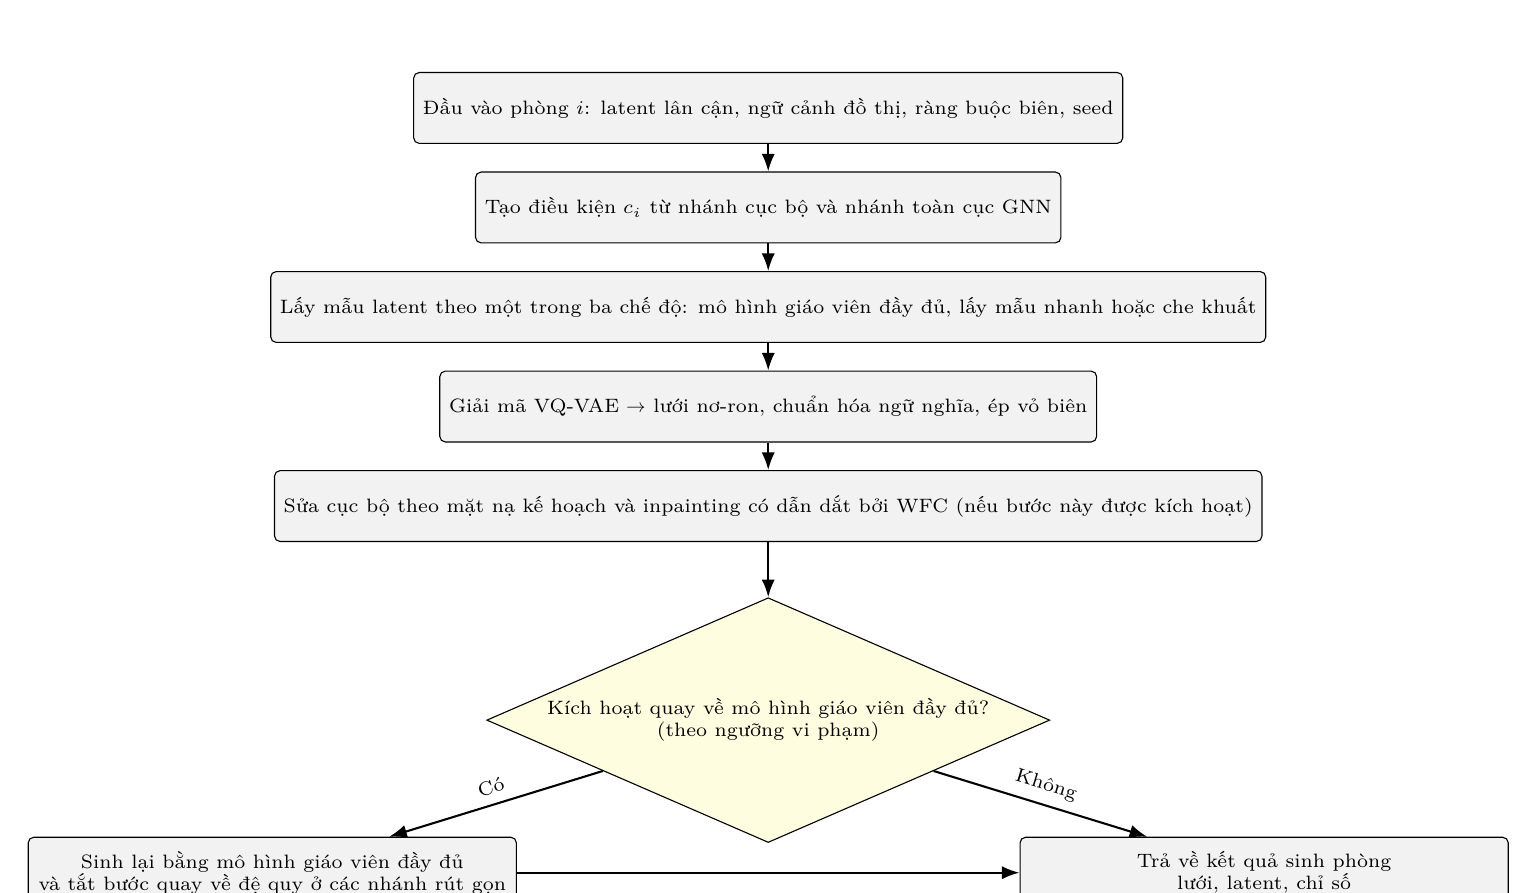
\begin{tikzpicture}[
  font=\scriptsize,
  >=Latex,
  node distance=3.5mm,
  flowstep/.style={draw, rounded corners=2pt, fill=gray!10, align=center, minimum width=6.2cm, minimum height=0.9cm},
  decision/.style={draw, diamond, aspect=2.3, align=center, inner sep=1.2pt, fill=yellow!12},
  arr/.style={->, line width=0.75pt}
]
  \node[flowstep] (in) {Đầu vào phòng $i$: latent lân cận, ngữ cảnh đồ thị, ràng buộc biên, seed};
  \node[flowstep, below=of in] (cond) {Tạo điều kiện $c_i$ từ nhánh cục bộ và nhánh toàn cục GNN};
  \node[flowstep, below=of cond] (sample) {Lấy mẫu latent theo một trong ba chế độ: mô hình giáo viên đầy đủ, lấy mẫu nhanh hoặc che khuất};
  \node[flowstep, below=of sample] (decode) {Giải mã VQ-VAE $\rightarrow$ lưới nơ-ron, chuẩn hóa ngữ nghĩa, ép vỏ biên};
  \node[flowstep, below=of decode] (repair) {Sửa cục bộ theo mặt nạ kế hoạch và inpainting có dẫn dắt bởi WFC (nếu bước này được kích hoạt)};
  \node[decision, below=7mm of repair] (fallback) {Kích hoạt quay về mô hình giáo viên đầy đủ?\\(theo ngưỡng vi phạm)};
  \node[flowstep, below left=7mm and 14mm of fallback] (teacher) {Sinh lại bằng mô hình giáo viên đầy đủ\\và tắt bước quay về đệ quy ở các nhánh rút gọn};
  \node[flowstep, below right=7mm and 14mm of fallback] (ret) {Trả về kết quả sinh phòng\\lưới, latent, chỉ số};

  \draw[arr] (in) -- (cond);
  \draw[arr] (cond) -- (sample);
  \draw[arr] (sample) -- (decode);
  \draw[arr] (decode) -- (repair);
  \draw[arr] (repair) -- (fallback);
  \draw[arr] (fallback) -- node[above, sloped]{Có} (teacher);
  \draw[arr] (fallback) -- node[above, sloped]{Không} (ret);
  \draw[arr] (teacher) -- (ret);
\end{tikzpicture}
}
\caption{Luồng nội bộ của quy trình sinh phòng, bao gồm bước hiệu chỉnh ký hiệu và bước quay về mô hình giáo viên.}
\label{fig:room_generation_flow}
\end{figure}

\begin{figure}[H]
\centering
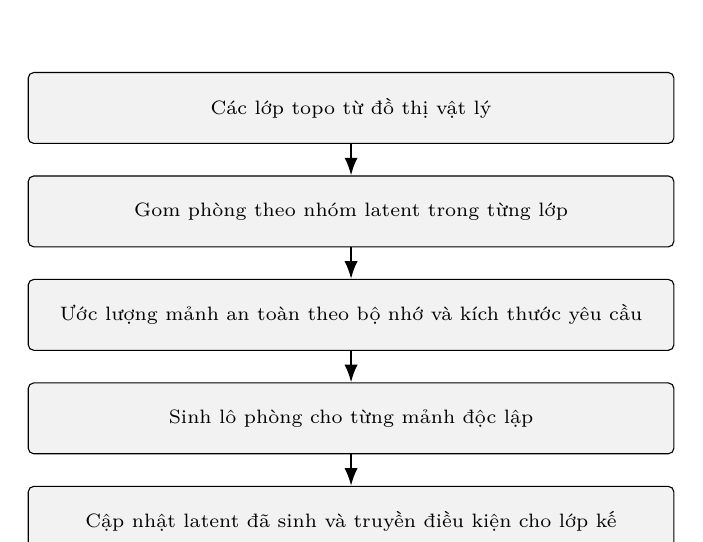
\begin{tikzpicture}[
  font=\scriptsize,
  >=Latex,
  node distance=4mm,
  box/.style={draw, rounded corners=2pt, fill=gray!10, align=center, minimum width=8.2cm, minimum height=0.9cm},
  arr/.style={->, line width=0.75pt}
]
  \node[box] (l0) {Các lớp topo từ đồ thị vật lý};
  \node[box, below=of l0] (l1) {Gom phòng theo nhóm latent trong từng lớp};
  \node[box, below=of l1] (l2) {Ước lượng mảnh an toàn theo bộ nhớ và kích thước yêu cầu};
  \node[box, below=of l2] (l3) {Sinh lô phòng cho từng mảnh độc lập};
  \node[box, below=of l3] (l4) {Cập nhật latent đã sinh và truyền điều kiện cho lớp kế};
  \draw[arr] (l0) -- (l1);
  \draw[arr] (l1) -- (l2);
  \draw[arr] (l2) -- (l3);
  \draw[arr] (l3) -- (l4);
\end{tikzpicture}
\caption{Luồng lập lịch sinh phòng theo lớp phụ thuộc và nhóm latent.}
\label{fig:layer_bucket_scheduler}
\end{figure}

\begin{algorithm}[H]
\caption{Lập lịch sinh phòng theo lớp phụ thuộc}
\label{alg:layer_bucket_scheduler}
\begin{algorithmic}[1]
\Require Đầu vào đã chuẩn bị $(G_{phys}, C)$, cấu hình sinh phòng
\Ensure Tập kết quả phòng $\mathcal{R}$, latent phòng và chẩn đoán batch
\If{chế độ batch phòng độc lập được kích hoạt và $G_{phys}$ có hướng}
  \State Phân lớp topo trên $G_{phys}$, thu $\mathcal{L}$
  \ForAll{lớp $\ell \in \mathcal{L}$}
    \State Gom các phòng trong $\ell$ theo nhóm latent, thu $\mathcal{B}$
    \ForAll{nhóm $b \in \mathcal{B}$}
      \If{kích thước phòng không chuẩn $(16,11)$}
        \State Sinh tuần tự từng phòng trong $b$
      \Else
        \State Ước lượng kích thước mảnh an toàn $k$ theo ngân sách bộ nhớ
        \ForAll{mảnh độc lập kích thước $k$ trong $b$}
          \State Sinh lô phòng cho mảnh hiện tại, thu $\mathcal{R}_{chunk}$
          \State Cập nhật $\mathcal{R}$ và latent đã sinh
        \EndFor
      \EndIf
    \EndFor
  \EndFor
\Else
  \State Sinh tuần tự theo thứ tự nút ổn định
\EndIf
\State \Return $\mathcal{R}$, latent phòng, chẩn đoán batch
\end{algorithmic}
\end{algorithm}

Bài toán sinh đa phòng được mô hình hóa như bài toán lập lịch có phụ thuộc thứ tự, do đó thuật toán tách xử lý theo lớp topo để bảo toàn quan hệ tiền nhiệm-hậu nhiệm. Trong từng lớp, các phòng được gom theo dạng latent và chia mảnh an toàn theo giới hạn bộ nhớ để tăng mức song song hóa mà không vi phạm ràng buộc logic. Nhánh tuần tự cho kích thước không chuẩn bảo đảm tính tương thích của quy trình.

\paragraph{Bảo toàn thứ tự phụ thuộc và chi phí lập lịch.}
Đối với bài toán lập lịch đa phòng, tính đúng được suy ra từ ba ràng buộc tổ
chức của thuật toán. Thứ nhất, phân lớp topo bảo toàn quan hệ tiền nhiệm --
hậu nhiệm giữa các phòng. Thứ hai, việc gom theo dạng latent ngăn các phòng có
hình dạng tensor không tương thích bị trộn chung trong một lô. Thứ ba, những
phòng không ở kích thước chuẩn được chuyển sang nhánh tuần tự để giữ đúng hợp
quy ước dữ liệu. Thuật toán kết thúc sau khi lần lượt duyệt hết tập lớp, tập nhóm
trong mỗi lớp và các mảnh độc lập của từng nhóm. Vì vậy, chi phí của phần lập
lịch là:
\begin{equation}
\mathcal{O}(n+m)+\mathcal{O}(N),
\end{equation}
và tổng chi phí sinh phòng là:
\begin{equation}
\sum_{b\in\mathcal{B}} \left\lceil\frac{|b|}{k_b}\right\rceil C_{\text{batch}}(k_b),
\end{equation}
với $k_b$ là kích thước mảnh an toàn của nhóm $b$.

\begin{algorithm}[H]
\caption{Suy luận dungeon theo quy trình lấy đồ thị làm trung tâm}
\label{alg:generate_dungeon_graph_first}
\begin{algorithmic}[1]
\Require Đồ thị nhiệm vụ tùy chọn $G$, siêu tham số suy luận $\Theta$
\Ensure Dungeon $D$, tập phòng $\mathcal{R}$, metrics $\mathcal{M}$
\If{$G=\varnothing$ và chế độ sinh cấu trúc đồ thị được bật}
  \State Sinh đồ thị nhiệm vụ bằng bộ sinh tiến hóa với siêu tham số $\Theta_{\text{graph}}$
\EndIf
\State Lọc nút ảo và dựng đồ thị vật lý $G_{\text{phys}}$
\State Dựng ngữ cảnh đồ thị, tensor điều kiện và ràng buộc biên cho từng phòng
\State Chia các phòng theo lớp topo và nhóm latent
\ForAll{bucket phòng độc lập}
  \State Sinh một lô phòng từ ngữ cảnh hiện tại dưới cấu hình $\Theta$
  \State Cập nhật latent đã sinh để cấp điều kiện cho lớp kế
\EndFor
\State Ghép các phòng đã sinh thành dungeon $D$
\If{bật đánh giá MAP-Elites}
  \State Tính các chỉ số quality--diversity trên dungeon $D$
\EndIf
\State \Return $(D,\mathcal{R},\mathcal{M})$
\end{algorithmic}
\end{algorithm}

Thuật toán điều phối toàn bộ quy trình lấy đồ thị làm trục chính từ khâu chuẩn bị đồ thị đến ghép dungeon và đánh giá chất lượng. Cách tổ chức theo các pha có quy ước dữ liệu rõ ràng giúp kiểm soát sai lệch xuyên tầng, đồng thời hỗ trợ thí nghiệm loại trừ và kiểm thử thành phần một cách hệ thống. Vì vậy, tính đúng đắn được bảo toàn ở cả cấp phòng lẫn cấp dungeon.

\paragraph{Tính nhất quán liên pha và chi phí toàn chuỗi.}
Xét ở cấp toàn quy trình, tính đúng phụ thuộc vào việc mỗi pha chỉ nhận đầu vào
đã được pha trước chuẩn hóa và thẩm định. Nếu không có đồ thị đầu vào, đồ thị
sinh mới phải vượt qua kiểm tra cấu trúc trước khi tham gia các bước sau; các
phòng phải được sinh theo thứ tự phụ thuộc trên đồ thị vật lý đã loại virtual
node; và các chỉ số hậu kỳ phải tách bạch giữa cấp phòng và cấp dungeon để
không trộn lẫn trách nhiệm chẩn đoán. Do số pha của quy trình là hữu hạn, toàn
bộ đường chạy dừng sau khi hoàn tất chuẩn bị đồ thị, sinh phòng theo nhóm và
mảnh, ghép dungeon và, khi được bật, đánh giá QD. Bởi vậy, độ phức tạp tổng
thể có thể viết:
\begin{equation}
\mathcal{O}\!\left(C_{\text{graph}} + C_{\text{rooms}} + C_{\text{stitch}} + C_{\text{eval}}\right),
\end{equation}
trong đó $C_{\text{graph}}$ được cho bởi Thuật toán \ref{alg:graph_evolution_feasible_first}.

\subsubsection{Luồng suy luận một phòng và bước quay về mô hình giáo viên}
Ở mức vi mô, một phòng được xử lý theo chuỗi dựng điều kiện $\rightarrow$ lấy mẫu latent $\rightarrow$ giải mã $\rightarrow$ sửa cục bộ. Bước quay về mô hình giáo viên đóng vai trò lớp an toàn, cho phép chuyển từ nhánh lấy mẫu nhanh sang nhánh chuẩn khi chỉ số vi phạm vượt ngưỡng thiết kế.

\begin{algorithm}[H]
\caption{Sinh một phòng với bước quay về mô hình giáo viên}
\label{alg:generate_room_fallback}
\begin{algorithmic}[1]
\Require Điều kiện phòng $(z_N,z_S,z_E,z_W,b_i,p_i,G_i)$, cấu hình bộ lấy mẫu
\Ensure Kết quả sinh phòng cho phòng $i$
\State $c_i \gets$ Kết hợp ngữ cảnh lân cận, ràng buộc biên và ngữ cảnh đồ thị
\If{chế độ suy luận là nhánh che khuất rời rạc}
  \State Lấy mẫu latent che khuất và phân bố dự đoán cho phòng, thu $(z_i,\ell_i)$
\ElsIf{chế độ suy luận là nhánh codebook rời rạc}
  \State Lấy mẫu theo tập mã rời rạc có điều kiện, thu $(z_i,\ell_i)$
\Else
  \State $z_i \gets$ Lấy mẫu latent bằng mô hình khuếch tán đầy đủ dưới CFG và dẫn dắt logic
  \State $\ell_i \gets$ Giải mã $z_i$ thành phân bố dự đoán trên lưới phòng
\EndIf
\State $x_i^{\text{neural}} \gets \arg\max\ell_i$
\State $x_i^{\text{final}} \gets$ Hiệu chỉnh ký hiệu và khôi phục vỏ biên từ $x_i^{\text{neural}}$
\If{cần quay về mô hình giáo viên}
  \State Sinh lại bằng mô hình giáo viên đầy đủ và vô hiệu hóa bước quay về lồng nhau
\EndIf
\State \Return $(x_i^{\text{final}}, z_i, \text{metrics})$
\end{algorithmic}
\end{algorithm}

Cách tổ chức này cân bằng chi phí suy luận với độ tin cậy cấu trúc bằng cách cho phép
các nhánh lấy mẫu nhanh hoạt động dưới giám sát hậu kiểm. Phòng được sinh theo
chuỗi điều kiện $\rightarrow$ lấy mẫu latent $\rightarrow$ giải mã $\rightarrow$
sửa cục bộ; sau đó bộ chỉ số vi phạm quyết định có cần kích hoạt bước quay về
mô hình giáo viên hay không. Nhờ vậy, những trường hợp vượt ngưỡng rủi ro được
tái sinh bằng một cấu hình ổn định hơn thay vì bị chấp nhận trực tiếp.

\paragraph{Điều kiện kích hoạt fallback và chi phí theo phòng.}
Ở cấp một phòng, quy trình bảo đảm tính đúng được tổ chức theo một chuỗi xử lý rõ
ràng: sinh đầu ra sơ bộ, thẩm định, rồi tái sinh khi thực sự cần thiết. Mọi đầu ra đều phải đi qua bước hiệu
chỉnh ký hiệu và kiểm tra biên; chỉ khi chỉ số vi phạm vượt ngưỡng thì nhánh
quay về mới kích hoạt để chuyển sang mô hình giáo viên ổn định hơn. Vì bước này
chỉ cho phép một lượt sinh chính và nhiều nhất một lượt tái sinh không đệ
quy, tiến trình luôn kết thúc sau số bước hữu hạn. Theo đó, độ phức tạp theo
phòng là:
\begin{equation}
\mathcal{O}\!\left(C_{\text{sample}} + C_{\text{decode}} + C_{\text{repair}} + \mathbb{I}_{\text{fb}}\,C_{\text{teacher}}\right).
\end{equation}

Để hạn chế rủi ro nhiễu cấu trúc từ các nhánh suy luận chi phí thấp hơn mô hình giáo viên, quy trình áp dụng một luật quay về tường minh. Với một phòng $r$, cờ quay về được viết gọn như sau:
\begin{equation}
\mathbb{I}_{\text{fallback}}(r)=\mathbf{1}\Big[
\begin{aligned}
&n_{\text{island}}\ge 1 \lor n_{\text{door-err}}\ge 1 \\
&\lor \big(n_{\text{repair}}\ge 18\land n_{\text{obs}}>0\big) \\
&\lor \big(m=\text{masked}\land (r_{\text{overwrite}}>0.34 \lor n_{\text{repair}}\ge 12)\big)
\end{aligned}
\Big].
\end{equation}
Khi điều kiện này đúng, phòng được sinh lại bằng mô hình khuếch tán đầy đủ ở vai trò mô hình giáo viên. Cách tổ chức này cho thấy hệ thống ưu tiên độ tin cậy của đầu ra hơn lợi ích tốc độ cục bộ của từng bộ lấy mẫu.

\subsection{Đánh giá sau sinh và chỉ số vận hành}
Sau khi ghép phòng, hệ thống không chuyển ngay lưới tổng hợp sang bộ giải, mà
trước hết đưa nó qua bước chuẩn hóa trước thẩm định. Bước này không chỉ điều
chỉnh hình dạng lưới, mà còn xác lập ranh giới rõ ràng giữa tầng sinh và tầng
thẩm định: đầu ra ghép được đưa về cùng một bộ từ vựng tile, các vùng
\texttt{VOID} kín bị loại bỏ, và cặp start-goal được chuẩn hóa về một cấu hình
duy nhất. Chỉ trên miền dữ liệu đã chuẩn hóa đó dungeon mới được chuyển sang
hai tầng hậu kiểm là bộ kiểm tra cơ học và P-CBS. Trong cấu trúc này,
MAP-Elites giữ vai trò đánh giá chất lượng--đa dạng ở cấp dungeon, còn
LogicNet được giữ như một kênh chẩn đoán ở cấp phòng thay vì làm tiêu chí quyết
định cuối cùng về tính chơi được.

Các chỉ số tổng hợp vận hành được ghi trực tiếp ở cuối đường sinh dungeon, trong đó có:
\begin{equation}
\mathrm{repair\_rate}=\frac{1}{N}\sum_{i=1}^{N} r_i,
\qquad
\mathrm{hard\_solvable\_rate}=\frac{1}{M}\sum_{j=1}^{M}\phi_{\mathrm{hard}}(D_j^{\star}),
\end{equation}
\begin{equation}
\begin{aligned}
\mathrm{pcbs\_success\_rate}
&=\frac{1}{M}\sum_{j=1}^{M}\phi_{\mathrm{pcbs}}(D_j^{\star}),\\
\mathrm{CGR}
&=
\frac{
\sum_{j=1}^{M}
\mathbf{1}\!\left[\phi_{\mathrm{hard}}(D_j^{\star})=1\right]
\mathbf{1}\!\left[\phi_{\mathrm{pcbs}}(D_j^{\star})=0\right]
}{
\sum_{j=1}^{M}\mathbf{1}\!\left[\phi_{\mathrm{hard}}(D_j^{\star})=1\right]
}.
\end{aligned}
\end{equation}
Ở đây $r_i=1$ nếu phòng $i$ có can thiệp sửa lỗi; $\phi_{\mathrm{hard}}$ là phán
quyết của bộ kiểm tra cơ học; còn $\phi_{\mathrm{pcbs}}$ là kết quả của P-CBS dưới
hồ sơ persona đang xét. Cách phân tầng chỉ số như trên giúp tách biệt ba nguồn
sai lệch khác nhau: sai lệch hình học ở cấp phòng, sai lệch tiến trình cơ học ở
cấp dungeon, và sai lệch nhận thức chỉ bộc lộ khi tác tử đánh giá bị ràng buộc
về trí nhớ, định hướng hoặc chiến lược khám phá.

\begin{algorithm}[H]
\caption{Đánh giá dungeon sau ghép với bước chuẩn hóa trước thẩm định, kiểm tra cơ học và P-CBS}
\label{alg:post_generation_evaluation}
\begin{algorithmic}[1]
\Require Dungeon đã ghép $D$, tập phòng $\mathcal{R}$, đồ thị vật lý $G_{phys}$, tập persona $\mathcal{P}$
\Ensure Chẩn đoán chuẩn hóa, phán quyết cơ học, chỉ số P-CBS, chỉ số QD và danh sách phòng lỗi
\State Chuẩn hóa dungeon trước thẩm định, thu $D^{\star}$ và $info_{\mathrm{handoff}}$
\State Kiểm tra cơ học trên $D^{\star}$, thu $s_{\mathrm{hard}}$
\If{$s_{\mathrm{hard}}$ giải được}
  \ForAll{$p \in \mathcal{P}$}
    \State Chạy P-CBS cho persona $p$, thu $m_p$
  \EndFor
  \If{bật MAP-Elites và thành phần MAP-Elites khả dụng}
    \State Cập nhật kho lưu trữ MAP-Elites bằng dungeon hợp lệ $D^{\star}$
    \State Trích xuất các chỉ số QD từ $D^{\star}$
  \EndIf
\EndIf
\If{LogicNet khả dụng}
  \ForAll{phòng $r_i \in \mathcal{R}$ có latent}
    \State Suy diễn LogicNet trên latent phòng, thu $(\ell_i,info_i)$
    \State Cộng dồn chỉ số chẩn đoán và ghi phòng lỗi nếu dưới ngưỡng
  \EndFor
\EndIf
\State \Return $info_{\mathrm{handoff}}, s_{\mathrm{hard}}, \{m_p\}_{p\in\mathcal{P}}$ cùng các chỉ số đánh giá và danh sách phòng lỗi
\end{algorithmic}
\end{algorithm}

Đánh giá hậu sinh vì vậy được phân tầng theo đúng vai trò của từng thành phần.
Oracle cứng quyết định dungeon có thỏa các điều kiện cơ học tối thiểu hay không.
P-CBS cho biết dungeon gây nhầm lẫn hoặc chậm trễ cho những persona nào.
MAP-Elites xác định vị trí của nghiệm trong không gian chất lượng--đa dạng, còn
LogicNet tiếp tục đóng vai trò chẩn đoán nội bộ ở mức phòng. Cách tách này
giúp các thí nghiệm loại trừ ở Chương 4 không còn trộn lẫn lỗi cơ học với lỗi
hành vi.

\paragraph{Thứ tự thẩm định và chi phí hậu sinh.}
Ở tầng đánh giá hậu sinh, tính đúng của quy trình được bảo đảm bởi thứ tự gọi
các bộ thẩm định. Dungeon chỉ được ghi vào kho lưu trữ khi đã vượt qua bộ kiểm tra cơ
học; P-CBS chỉ làm việc trên lưới đã qua chuẩn hóa trước thẩm định; còn LogicNet chỉ
giữ vai trò chẩn đoán trên những phòng còn latent. Điều kiện dừng tương ứng với
việc hoàn tất hữu hạn bốn bước: chuẩn hóa lưới ghép, thẩm định cơ học, duyệt
tập persona và duyệt tập phòng có latent. Vì vậy, độ phức tạp là:
\begin{equation}
\mathcal{O}\!\left(
C_{\mathrm{handoff}}(D)+
C_{\mathrm{hard}}(D,G)+
|\mathcal{P}|\,C_{\mathrm{pcbs}}(D)+
N_z\,C_{\mathrm{logicnet}}+
C_{\mathrm{archive}}
\right).
\end{equation}

\subsection{Giả định vận hành, chế độ lỗi và biện pháp giảm thiểu}
\paragraph{Giả định vận hành.}
Mô tả phương pháp trong chương này dựa trên ba giả định vận hành cơ bản: (i) đồ thị vật lý sau khi lọc nút ảo vẫn liên thông và có cặp start-goal hợp lệ, (ii) phòng đầu vào/đầu ra tuân thủ quy ước kích thước và từ vựng tile, và (iii) lưới ghép trước bộ thẩm định luôn đi qua bước chuẩn hóa trước thẩm định để loại token ngoài bảng từ điển và chuẩn hóa terminal. Viết gọn:
\begin{equation}
\mathrm{Connected}(G_{\mathrm{phys}})=1,\qquad s,g\in V_{G_{\mathrm{phys}}},\ s\neq g,
\end{equation}
\begin{equation}
x_i\in\{0,\ldots,43\}^{16\times 11},\qquad
r_d\le h_d\ \ (d\in\{N,S,E,W\}).
\end{equation}
Các giả định này không thay cho đánh giá thực nghiệm, nhưng giúp xác định rõ miền hiệu lực của các thuật toán ở Mục 3.4.

\paragraph{Chế độ lỗi và giảm thiểu.}
Bảng~\ref{tab:failure_modes_ch3} tóm tắt các lỗi vận hành thường gặp và hướng xử lý tương ứng trong quy trình.

\begin{table}[H]
\centering
\caption{Các chế độ lỗi chính và hướng xử lý trong đường chạy Chương 3}
\label{tab:failure_modes_ch3}
\begin{tabular}{>{\raggedright\arraybackslash}p{3.0cm} >{\raggedright\arraybackslash}p{4.7cm} >{\raggedright\arraybackslash}p{5.1cm}}
\toprule
Nhóm lỗi & Biểu hiện quan sát được & Hướng xử lý trong quy trình \\
\midrule
Sai lược đồ tensor & Lỗi kích thước ở tầng điều kiện hóa hoặc trong lô khuếch tán. & Dừng sớm tại điểm vào khối $B_3/B_4$, kiểm tra kiểu--kích thước trước khi lấy mẫu. \\
Đồ thị không khả thi & Đồ thị vi phạm ràng buộc tiến trình hoặc không đạt điều kiện hậu kiểm. & Chọn nghiệm khả thi-ưu tiên, phạt vi phạm mềm, hậu kiểm tra trước khi ghép phòng. \\
Nhiễu cấu trúc từ bộ lấy mẫu nhanh & Xuất hiện island, lỗi cửa, hoặc overwrite cao ở chế độ masked. & Luật quay về mô hình giáo viên theo ngưỡng vi phạm, đồng thời chặn quay về đệ quy. \\
Lệch biên-cửa sau giải mã & Cửa bắt buộc mất hoặc biên ngoài không kín. & Ép lớp biên, sửa theo mặt nạ kế hoạch, inpainting có dẫn dắt bởi WFC. \\
Rò rỉ \texttt{VOID}/token ngoài bảng từ điển & Lưới ghép chứa ô không hợp lệ hoặc \texttt{VOID} kín làm sai phán quyết bộ thẩm định. & Bắt buộc chạy bước chuẩn hóa trước thẩm định: ánh xạ lại semantic ID, lấp \texttt{VOID} kín, chuẩn hóa đúng một start-goal. \\
Suy giảm thành phần phụ trợ & LogicNet, MAP-Elites hoặc nhánh P-CBS tạm không khả dụng ở một số cấu hình loại trừ. & Chạy suy giảm có kiểm soát: giữ bộ kiểm tra cơ học làm chuẩn tối thiểu, tách rõ chỉ số nào bị vô hiệu hóa. \\
\bottomrule
\end{tabular}
\end{table}

\section{Cấu hình triển khai và khả năng tái lập}
Cấu hình chuẩn được quản lý tập trung trong bộ tham số thí nghiệm, trong đó các tham số lõi như kích thước phòng, số lớp tile, số chiều latent, hệ số CFG, số bước diffusion và cờ bật/tắt repair đều được khai báo tường minh. Seed được đồng bộ cho các thành phần sinh ngẫu nhiên chính của hệ thống; trong thiết lập phân tán, mỗi worker dùng seed lệch theo chỉ số tiến trình để tách luồng ngẫu nhiên nhưng vẫn bảo toàn khả năng truy vết. Hệ điểm kiểm tra được tổ chức theo giai đoạn, lưu kèm siêu dữ liệu kiến trúc và trạng thái huấn luyện, đồng thời dùng chiến lược lưu an toàn để giảm nguy cơ hỏng điểm kiểm tra trong các phiên chạy dài.

Về tiêu chí dừng, tầng cấu trúc đồ thị nhiệm vụ có thể dừng sớm khi fitness hội tụ; tầng diffusion dừng theo số epoch cấu hình và chọn điểm kiểm tra theo chỉ số xác thực; tầng suy luận dừng theo số phòng cùng giới hạn số vòng sửa lỗi. Cách tổ chức này tạo ra đường chạy nhất quán giữa huấn luyện và suy luận, đồng thời giữ chi phí tính toán trong ngưỡng phù hợp với quy mô dữ liệu hiện có.

\section{Liên kết với yêu cầu thiết kế và thiết kế thực nghiệm}
Để bảo đảm Chương 3 bám sát trật tự vận hành của hệ thống, các nội dung được sắp theo đúng chuỗi trả lời cho các yêu cầu R1--R5. Mục 3.2 làm rõ hai lớp đồ thị, ma trận đầu vào--đầu ra theo khối, luồng dữ liệu, tiền xử lý và các bất biến vận hành để trả lời R1, R2 và R5. Mục 3.3 đi vào quyết định thiết kế của từng khối để hiện thực hóa R1--R4: từ sinh đồ thị nhiệm vụ, biểu diễn latent, điều kiện hóa từ đồ thị sang phòng, khuếch tán có điều kiện, sửa lỗi ký hiệu cho đến tầng hậu kiểm. Mục 3.4 mô tả huấn luyện, suy luận và hậu kiểm theo đúng trật tự vận hành thực tế để cho thấy các yêu cầu trên được duy trì như thế nào khi hệ thống chạy thật; còn Mục 3.5 khép lại bằng cấu hình triển khai và tái lập nhằm bảo vệ R5.

Ở mức kiểm chứng, cấu trúc này cũng tạo điều kiện cho phân tích loại trừ theo từng khối: tiên nghiệm cấu trúc đồ thị (Khối I), điều kiện hóa (Khối III), diffusion (Khối IV), hướng dẫn logic (Khối V), sửa lỗi ký hiệu (Khối VI) và lớp hậu kiểm gồm kiểm tra cơ học, P-CBS và QD (Khối VII). Vì mỗi khối có giao diện rõ ràng và cờ bật/tắt độc lập, thí nghiệm ở Chương 4 có thể ước lượng minh bạch đóng góp biên của từng quyết định thiết kế dưới cùng ngân sách vận hành. Việc đặt các nhánh giáo viên, nhanh và che khuất trong cùng một quy trình, kèm bước kẹp guidance theo miền chưng cất, cũng giúp so sánh công bằng hơn giữa chất lượng và chi phí. Đồng thời, chuẩn hóa seed, điểm kiểm tra và ghi log cho phép triển khai đồng thời ba nhóm kiểm chứng: kiểm tra cơ học, bộ kiểm thử persona và đánh giá OOD/thống kê theo cặp (bootstrap và FDR) với độ lặp lại cao \cite{efron1994bootstrap,benjamini1995fdr}.

\section{Tóm tắt chương}
Chương 3 đã đặc tả đầy đủ quy trình nơ-ron--ký hiệu theo hướng lấy đồ thị làm trung tâm ở mức triển khai: từ biểu diễn dữ liệu, cách điều kiện hóa từ đồ thị sang phòng, công thức huấn luyện/suy luận của diffusion, đến các lớp sửa lỗi, bước chuẩn hóa trước thẩm định và lớp hậu kiểm gồm kiểm tra cơ học, P-CBS và QD. Điểm cốt lõi của phương pháp là tách trách nhiệm theo tầng nhưng liên kết bằng một quy ước dữ liệu thống nhất; nhờ đó hệ thống vừa kiểm soát được tiến trình toàn cục, vừa duy trì chất lượng hình học ở mức cục bộ và đo được ma sát nhận thức ở mức persona. Trên nền đặc tả này, Chương 4 có cơ sở để đánh giá định lượng đóng góp của từng thành phần trong các thiết lập cùng ngân sách và OOD.

\chapter{Kết quả thực nghiệm và thảo luận}
Chương này trình bày kế hoạch thực nghiệm và khung phân tích kết quả theo đúng các trục kiểm chứng đã thiết kế ở Chương 1 và Chương 3. Nội dung được tổ chức theo mạch: mục tiêu kiểm chứng \rightarrow thiết kế giao thức \rightarrow kết quả định lượng \rightarrow thảo luận kết quả và giới hạn.

\section{Mục tiêu kiểm chứng và câu hỏi thực nghiệm}
Phần này đặt lại các câu hỏi nghiên cứu ở dạng kiểm chứng thực nghiệm để làm rõ tiêu chí đánh giá thành công của phương pháp:
\begin{enumerate}[label=(RQ\arabic*)]
  \item Cấu hình nơ-ron--ký hiệu lấy đồ thị làm trung tâm có cải thiện đồng thời tính hợp lệ gameplay, khả năng giải được và chất lượng phòng so với các cấu hình đối chứng hay không?
  \item Đóng góp biên của từng khối (tiên nghiệm cấu trúc đồ thị, điều kiện hóa, diffusion, hướng dẫn logic, sửa lỗi ký hiệu, bước quay về mô hình giáo viên) có ý nghĩa thống kê hay không?
  \item Khi bị ràng buộc cùng ngân sách đánh giá, phương pháp đề xuất có giữ lợi thế so với các cấu hình đối chứng sinh đồ thị nhiệm vụ hay không?
  \item Hiệu năng có duy trì ổn định trên các kịch bản OOD-small và OOD-large, tức các miền kiểm tra có quy mô và cấu trúc lệch khỏi phân phối huấn luyện, hay không?
\end{enumerate}

Trong phần trình bày dưới đây, mỗi câu hỏi được gắn với một nhóm chỉ số riêng để tránh đánh giá cảm tính. RQ1 được kiểm tra bằng các chỉ số khả thi, hợp lệ ràng buộc, mức sửa hậu kỳ, thời lượng sinh và các thước đo khả giải; RQ2 dùng paired bootstrap và kiểm định hoán vị dấu theo cặp trên các chỉ số chính; RQ3 đọc theo giao thức đồng ngân sách với cùng số lần đánh giá; RQ4 xem chênh lệch khi chuyển từ ID sang OOD-small/OOD-large \cite{efron1994bootstrap,benjamini1995fdr}. Nhờ vậy, các kết luận ở cuối chương có thể truy ngược về đúng thước đo mà nó phụ thuộc.
Trong phiên bản hoàn chỉnh của giao thức, các thước đo còn được nhóm theo hai lớp kiểm chứng khác nhau. Lớp \emph{cơ học} trả lời dungeon có đúng cơ học hay không thông qua tỉ lệ giải được theo bộ kiểm tra cơ học, mức hợp lệ của tiến trình, tỉ lệ không rơi vào soft-lock và các chỉ số sửa lỗi hoặc vi phạm biên. Lớp \emph{nhận thức} trả lời dungeon gây ma sát như thế nào đối với persona thông qua tỉ lệ thành công của P-CBS, chỉ số CGR, entropy điều hướng và \emph{goal-sighting latency}. Cách tách này giúp RQ1 và RQ2 không còn đánh đồng ``có lời giải'' với ``dễ điều hướng''.

\section{Thiết kế thực nghiệm}
\subsection{Thiết lập tái lập và môi trường thực nghiệm}
Mục này nêu chi tiết phần cứng, phần mềm, phiên bản thư viện, seed, chiến lược checkpoint và cách ghi vết. Các cấu hình được cố định để bảo đảm mỗi thí nghiệm có thể chạy lại và đối chiếu trực tiếp.

\begin{table}[H]
\centering
\small
\caption{Cấu hình máy dùng cho các thí nghiệm huấn luyện và đánh giá}
\label{tab:training_machine}
\begin{tabular}{>{\raggedright\arraybackslash}p{4.0cm} >{\raggedright\arraybackslash}p{9.0cm}}
\toprule
Thành phần & Thông số \\
\midrule
CPU & 12th Gen Intel(R) Core(TM) i5-12500H, $12$ nhân, $16$ luồng, xung cơ bản $2.50$ GHz \\
GPU & NVIDIA GeForce RTX 3050 Ti Laptop GPU, bộ nhớ đồ họa xấp xỉ $4$ GB, CUDA $12.4$ \\
RAM & $16$ GB RAM hệ thống (khả dụng khoảng $15.73$ GB) \\
Hệ điều hành & Microsoft Windows 11 Home Single Language, bản dựng $26200$, kiến trúc $64$ bit \\
Môi trường học sâu & Python $3.13.7$, PyTorch $2.6.0{+}$cu124 \\
\bottomrule
\end{tabular}
\end{table}

Toàn bộ các lần chạy trọng tâm trong khóa luận được quản lý trên cùng lớp phần cứng ở Bảng~\ref{tab:training_machine}. Để bảo đảm tái lập, luồng đánh giá giữ nguyên seed, checkpoint và cấu hình sinh trong mỗi lần chạy. Mỗi mẫu sinh đều ghi nhận thời lượng thực thi toàn chuỗi, số tile phải sửa, số marker đồ thị bị ghi đè và các chẩn đoán hậu kiểm, nhờ đó kết quả không chỉ phản ánh chất lượng đầu ra mà còn phản ánh chi phí vận hành thực. Với các so sánh nội bộ, cấu trúc đồ thị nhiệm vụ và vị trí phòng được giữ cố định để giảm nhiễu do thay đổi đầu vào.

\subsection{Dữ liệu và kịch bản đánh giá}
Mục này mô tả corpus dùng để huấn luyện, đơn vị chia tập thực tế trong mã nguồn và cách dựng các kịch bản đánh giá ID, OOD-small, OOD-large.

Corpus thực nghiệm là tập Zelda đã chuẩn hóa ở Chương 3, gồm $18$ dungeon nguồn tương ứng với $9$ dungeon và $2$ biến thể nhiệm vụ cho mỗi dungeon. Sau bước đối sánh giữa lưới và đồ thị nhiệm vụ, hệ thống trích được $459$ mẫu phòng chuẩn $16\times 11$ để dùng cho các mô hình học ở mức phòng. Trong các nhánh VQ-VAE, nhánh sinh nhanh và nhánh che khuất, việc chia tập được thực hiện sau khi trộn xác định theo seed, với tỉ lệ $90/10$, tương ứng $413$ mẫu huấn luyện và $46$ mẫu kiểm định nội bộ. Cách chia này phản ánh đúng đơn vị học trực tiếp của mô hình là từng phòng, đồng thời vẫn bảo đảm tái lập do thứ tự trộn được cố định.

Riêng với nhánh khuếch tán chính ở cấu hình hiện tại, bộ nạp dữ liệu được khởi tạo trên toàn bộ corpus thay vì duy trì một tập giữ lại độc lập ngay trong vòng huấn luyện. Vì vậy, khóa luận không dùng loss nội bộ của nhánh này như bằng chứng kết luận cuối cùng. Thay vào đó, kết quả được đọc chủ yếu qua giao thức hậu kiểm sau sinh, so sánh đồng ngân sách và các phép thử OOD ở cấp dungeon. Cách trình bày này giúp phần thực nghiệm bám đúng hành vi hiện thực của hệ thống thay vì mô tả một cách chia tập không tồn tại trong mã nguồn.

Trong chương này, ID (\emph{in-distribution}) chỉ các cấu hình kiểm tra còn gần với phân phối huấn luyện về số phòng, độ sâu tiến trình và mật độ phân nhánh; ngược lại, OOD (\emph{out-of-distribution}, ngoài phân phối) chỉ các cấu hình đã lệch đáng kể theo một hoặc nhiều trục trên. Cụ thể, OOD-small làm giảm quy mô dungeon hoặc độ sâu tiến trình để đo độ bền ở các cấu trúc nhỏ hơn; còn OOD-large tăng số phòng, độ sâu và mức phân nhánh để quan sát khả năng giữ nhất quán khi ngoại suy. Nhờ tách riêng ba kịch bản này, Chương 4 có thể phân biệt rõ hiện tượng mô hình chỉ tái hiện tốt trên miền quen thuộc với hiện tượng mô hình vẫn duy trì được tiến trình và tính chơi được khi quy mô dungeon thay đổi.

\subsection{Cấu hình đối chứng và cấu hình so sánh}
Mục này liệt kê các cấu hình đối chứng theo từng tầng (sinh đồ thị, sinh phòng, sửa lỗi), cùng các cấu hình loại trừ bật/tắt từng khối trong quy trình đề xuất để bảo đảm so sánh công bằng.

Ở tầng sinh đồ thị nhiệm vụ, bộ so sánh chuẩn gồm cấu hình ngẫu nhiên, chiến lược tiến hóa, giải thuật di truyền, MAP-Elites và cấu hình đầy đủ; các nhãn kỹ thuật tương ứng được giữ trong bảng để thuận tiện đối chiếu. Ở tầng sinh phòng, ba nhánh chính lần lượt đại diện cho đường khuếch tán chuẩn, đường lấy mẫu rút gọn và đường che khuất toàn phòng, qua đó tách riêng ảnh hưởng của số bước lấy mẫu và bước hậu xử lý. Ở tầng sửa lỗi, các thí nghiệm loại trừ bỏ TPE hoặc làm yếu tín hiệu đồ thị cho thấy tác động của mã hóa theo thứ tự topo và cơ chế cross-attention trên cùng một cấu trúc đầu vào. Cách tổ chức này bảo đảm mỗi cấu hình đối chứng trả lời một câu hỏi khác nhau thay vì chồng lấn trách nhiệm.

\subsection{Siêu tham số chính dùng trong Chương 4}
Để tránh thiếu nhất quán giữa mô tả và hiện thực, các siêu tham số cốt lõi trong chương này được neo trực tiếp vào cấu hình chuẩn của hệ thống và vào chính bộ chạy Block~I đã dùng để tạo hình trong phần kết quả. Bảng~\ref{tab:chapter4_core_hyperparams} liệt kê các giá trị được dùng xuyên suốt khi không có ghi chú ngoại lệ trong từng thí nghiệm.

\begin{table}[H]
\centering
\small
\setlength{\tabcolsep}{4pt}
\renewcommand{\arraystretch}{1.08}
\caption{Siêu tham số lõi của giao thức Chương 4}
\label{tab:chapter4_core_hyperparams}
\resizebox{\textwidth}{!}{%
\begin{tabular}{>{\raggedright\arraybackslash}p{3.2cm} >{\raggedright\arraybackslash}p{3.8cm} >{\raggedright\arraybackslash}p{6.2cm}}
\toprule
Nhóm & Tham số & Giá trị dùng trong báo cáo \\
\midrule
VQ-VAE (Khối II) & Chiều latent; độ rộng ẩn; kích thước codebook & $64$; $96$; $256$ (nhánh đối sánh có thêm biến thể $512$) \\
VQ-VAE (huấn luyện) & Tốc độ học; batch size; số epoch & $3\times 10^{-4}$; $4$; $300$ \\
Diffusion (Khối IV) & Số kênh nền; chiều ngữ cảnh; chiều ẩn điều kiện; số bước nhiễu & $96$; $256$; $192$; $1000$ \\
Diffusion (huấn luyện) & Tốc độ học; số epoch; ngưỡng Min-SNR; số epoch warmup & $10^{-4}$; $100$; $5.0$; $5$ \\
Diffusion (suy luận) & Hệ số CFG; số bước lấy mẫu; xác suất bỏ điều kiện puzzle & $3.0$; $50$; $0.35$ (có sweep ở Bảng~\ref{tab:pdrop_sweep_results}) \\
Mã hóa đồ thị (Khối III) & Kiến trúc GNN; số lớp GNN; chiều nút/cạnh/TPE & GPS; $2$; $14/16/8$ \\
Repair và puzzle control & Số lượt repair tối đa; block budget mỗi phòng; số ứng viên puzzle; ngân sách validator & $5$; $28$; $4$; $512$ \\
Run end-to-end thật & Seed; số phòng; population; generations của Block I & $20260418$; $12$; $24$; $24$ \\
Ngân sách search suite & A*; BFS/Dijkstra/Greedy; D* Lite; DFS/IDDFS & $200{,}000$; $50{,}000$; $100{,}000$; $100{,}000$ trạng thái \\
Đánh giá thống kê & Bootstrap ghép cặp; hoán vị dấu theo cặp; hiệu chỉnh FDR & CI bootstrap $95\%$; giá trị $p$; Benjamini--Hochberg \\
\bottomrule
\end{tabular}
}
\end{table}

\subsection{Chỉ số đánh giá và suy luận thống kê}
Mục này đặc tả bộ chỉ số chính và cách diễn giải chúng trong từng lớp kiểm chứng. Một chỉ số chỉ được dùng để kết luận đúng lớp mà nó đo: chỉ số cơ học không thay cho chỉ số nhận thức, còn độ mới hay QD-score không thay cho tính hợp lệ tiến trình. Suy luận thống kê dùng paired bootstrap để ước lượng khoảng tin cậy, kiểm định hoán vị dấu theo cặp để ước lượng giá trị $p$, và hiệu chỉnh Benjamini--Hochberg FDR để giảm nguy cơ kết luận dương tính giả khi phải so sánh nhiều cột số liệu \cite{efron1994bootstrap,benjamini1995fdr}.

Các chỉ số được đọc theo năm lớp: hợp lệ cơ học, ma sát nhận thức, hình thái và tiến trình, đa dạng, và chi phí. Với chỉ số điều kiện theo loại cửa hoặc cổng, khi cấu trúc đồ thị không chứa loại gate tương ứng thì giá trị $1.0$ phải được hiểu là ``không phát sinh vi phạm trên điều kiện có mặt'', chứ không phải lợi thế tuyệt đối của mô hình. Tương tự, độ mới cao chỉ cho biết đầu ra khác mẫu tham chiếu hơn; nó không tự động đồng nghĩa với tốt hơn nếu đồng thời làm suy giảm tính hợp lệ hoặc khả giải. Phần chi phí luôn được tính trên toàn bộ chuỗi xử lý, vì thời gian cuối cùng còn bao gồm sửa lỗi, phủ lại marker, kiểm tra cơ học và thẩm định nhận thức.

\begin{longtable}{>{\raggedright\arraybackslash}p{0.23\textwidth} >{\raggedright\arraybackslash}p{0.17\textwidth} >{\raggedright\arraybackslash}p{0.50\textwidth}}
\caption{Diễn giải các chỉ số chính dùng trong Chương 4}
\label{tab:metric_interpretation}\\
\toprule
Chỉ số & Cách đọc & Ý nghĩa và lưu ý diễn giải \\
\midrule
\endfirsthead
\toprule
Chỉ số & Cách đọc & Ý nghĩa và lưu ý diễn giải \\
\midrule
\endhead
Hard-solvable / bộ kiểm tra cơ học & Đạt hoặc tỉ lệ, càng cao càng tốt & Dungeon vượt toàn bộ lớp kiểm tra cơ học: tiến trình đúng, reachability hợp lệ và không rơi vào soft-lock. Đây là cổng tối thiểu trước khi bàn sang tầng nhận thức. \\
P-CBS chấp nhận & Đạt hoặc tỉ lệ, càng cao càng tốt & Persona đạt được mục tiêu trong khi vẫn nằm trong ngân sách nhận thức đã quy định. Chỉ số này chỉ được đọc trên các dungeon đã vượt qua bộ kiểm tra cơ học. \\
CGR & Tỉ lệ, càng thấp càng tốt & Phần trăm dungeon ``đúng cơ học nhưng khó hiểu với persona'', tức bộ kiểm tra cơ học đạt nhưng P-CBS thất bại. Chỉ số này đo độ lệch giữa lớp cơ học và lớp nhận thức. \\
$H_{\mathrm{nav}}$ & Số thực, càng thấp càng tốt & Entropy điều hướng dọc theo quỹ đạo của persona. Giá trị cao cho thấy phân bố di chuyển bị dàn rộng, thường đi kèm hiện tượng quay lui hoặc dò đường thiếu chắc chắn. \\
\emph{Goal-sighting Latency} & Số bước, càng thấp càng tốt & Độ trễ nhận thức mục tiêu: khoảng bước từ khi persona lần đầu tiên nhìn thấy hoặc nhận diện được affordance/mục tiêu tới khi đạt được. Phản ánh khả năng khai thác thông tin không gian; giá trị thấp chỉ ra persona tìm được con đường hiệu quả sau khi phát hiện. \\
Tỉ lệ phòng phải sửa & Tỉ lệ, càng thấp càng tốt & Phần trăm phòng mà bước sửa ký hiệu hoặc hậu xử lý phải can thiệp. Giá trị cao cho thấy nhánh sinh còn phụ thuộc nhiều vào lớp sửa lỗi. \\
Ghi đè marker & Tỉ lệ, càng thấp càng tốt & Tỉ lệ marker tiến trình bị đầu ra nơ-ron làm sai hoặc làm mất trước khi lớp phủ ký hiệu khôi phục lại. Chỉ số này phản ánh mức lệch giữa hình học sinh ra và ngữ nghĩa đồ thị. \\
NCD gần tham chiếu & Khoảng cách, càng thấp càng tốt & Khoảng cách nén giữa đầu ra và mẫu tham chiếu gần nhất. Giá trị thấp nghĩa là giống dữ liệu nguồn hơn, nhưng không đủ để kết luận chất lượng gameplay nếu thiếu các chỉ số cơ học và nhận thức. \\
GED gần tham chiếu & Khoảng cách, càng thấp càng tốt & Khoảng cách chỉnh sửa đồ thị xấp xỉ giữa đồ thị sinh ra và mẫu tham chiếu gần nhất ở tầng đồ thị nhiệm vụ. Chỉ số này hữu ích để đọc độ khác hình thái cấu trúc, nhưng không thay thế cho kiểm tra hợp lệ tiến trình. \\
Điểm thích nghi & Số thực, càng cao càng tốt & Điểm fitness tổng hợp ở tầng đồ thị nhiệm vụ. Chỉ nên so sánh trong cùng một thiết lập kiểm thử và cùng hàm mục tiêu, vì điểm này phụ thuộc mạnh vào cách chuẩn hóa tiêu chí. \\
Hợp lệ vận hành & Tỉ lệ, càng cao càng tốt & Tỉ lệ đầu ra sau hậu xử lý chuẩn vẫn đủ điều kiện để đi tiếp sang tầng kế tiếp của quy trình. Ở tầng đồ thị nhiệm vụ, chỉ số này giúp phân biệt giữa đồ thị đạt điểm tốt trên một vài bộ mô tả với đồ thị thật sự dùng được cho bước sinh ở tầng sau. \\
Hoàn chỉnh tổng thể & Tỉ lệ, càng cao càng tốt & Phần trăm đồ thị nhiệm vụ sinh ra đạt được bộ điều kiện tối thiểu để đi hết chuỗi tiến trình đã thiết kế. Đây là chỉ số tổng hợp ở tầng kiểm thử đồ thị. \\
Hợp lệ ràng buộc & Tỉ lệ, càng cao càng tốt & Phần trăm đồ thị không vi phạm các luật khóa--cổng, item-gate, boss gate hoặc các cổng có trạng thái. Chỉ số này đặc biệt quan trọng trong các thí nghiệm OOD. \\
Độ mới & Số thực, càng cao càng tốt theo nghĩa đa dạng & Mức khác biệt trung bình giữa nghiệm hiện tại và các nghiệm lân cận hoặc kho tham chiếu. Chỉ số này phải được đọc song song với tính hợp lệ để tránh đánh đồng ``mới'' với ``dùng được''. \\
Coverage / QD-score & Tỉ lệ và điểm tổng hợp, càng cao càng tốt & Coverage đo phần trăm ô trong kho lưu trữ đã có nghiệm ưu tú; QD-score cộng dồn chất lượng của các nghiệm ưu tú hiện có. Hai chỉ số này cho biết hệ vừa lấp rộng không gian hành vi đến đâu, vừa giữ chất lượng trung bình ra sao. \\
Thời gian (s) & Càng thấp càng tốt & Thời lượng đầu-cuối của toàn bộ quy trình, bao gồm lấy mẫu, sửa hậu kỳ, phủ marker, kiểm tra cơ học và thẩm định P-CBS nếu được bật. Vì vậy, chỉ số này không được đồng nhất với riêng tốc độ của bộ lấy mẫu. \\
\bottomrule
\end{longtable}

\subsection{Tách lớp đánh giá cơ học và ma sát nhận thức}
Để tránh diễn giải quá mạnh từ một bộ solve duy nhất, giao thức đánh giá của khóa luận được phân tầng theo bốn lớp kế tiếp như trong Hình~\ref{fig:chapter4_evaluation_layers}. Lớp đầu tiên trả lời câu hỏi cơ học tối thiểu: dungeon có đúng tiến trình và không rơi vào soft-lock hay không. Chỉ các dungeon vượt qua lớp này mới đi tiếp sang lớp nhận thức, nơi P-CBS và các hồ sơ persona đo mức do dự, quay lui và khó khăn điều hướng. Sau đó mới đến lớp chất lượng--đa dạng và cuối cùng là lớp robust/statistics để so sánh matched-budget, OOD và suy luận thống kê theo cặp.

\begin{figure}[H]
\centering
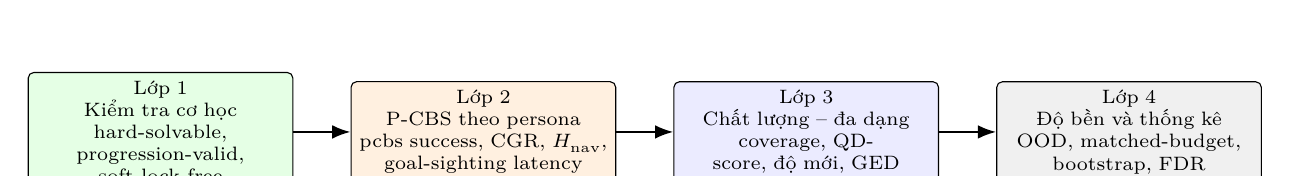
\begin{tikzpicture}[
  font=\scriptsize,
  >=Latex,
  layerbox/.style={draw, rounded corners=2pt, align=center, text width=3.15cm, minimum height=1.15cm, inner sep=3pt},
  arr/.style={->, line width=0.8pt}
]
\node[layerbox, fill=green!10] (l1) at (0,0) {Lớp 1\\Kiểm tra cơ học\\hard-solvable, progression-valid, soft-lock-free};
\node[layerbox, fill=orange!12] (l2) at (4.1,0) {Lớp 2\\P-CBS theo persona\\pcbs success, CGR, $H_{\mathrm{nav}}$, goal-sighting latency};
\node[layerbox, fill=blue!8] (l3) at (8.2,0) {Lớp 3\\Chất lượng -- đa dạng\\coverage, QD-score, độ mới, GED};
\node[layerbox, fill=gray!12] (l4) at (12.3,0) {Lớp 4\\Độ bền và thống kê\\OOD, matched-budget, bootstrap, FDR};
\draw[arr] (l1) -- (l2);
\draw[arr] (l2) -- (l3);
\draw[arr] (l3) -- (l4);
\end{tikzpicture}
\caption{Khung kiểm chứng nhiều lớp của Chương 4: tách đúng cơ học, ma sát nhận thức, chất lượng--đa dạng và độ bền thống kê.}
\label{fig:chapter4_evaluation_layers}
\end{figure}

Với cách đọc này, một dungeon chỉ được xem là ``tốt'' khi đồng thời (i) vượt bộ kiểm tra cơ học, (ii) không tạo ra độ vênh nhận thức quá cao ở các persona mục tiêu, và (iii) vẫn nằm ở vùng có chất lượng--đa dạng chấp nhận được. Điều này trực tiếp hiện thực hóa yêu cầu R4 đã nêu ở Chương 3.

\subsection{Hồ sơ persona và phạm vi báo cáo của P-CBS}
Ba hồ sơ persona chuẩn hóa của khóa luận đã được cố định ở Chương 3 trong Bảng~\ref{tab:pcbs_persona_profiles}: \emph{novice}, \emph{balanced} và \emph{speedrunner}. Ba hồ sơ này không khác nhau ở không gian trạng thái hay luật chơi, mà khác nhau ở dung lượng trí nhớ làm việc, thiên hướng tiến đích và mức phạt cho quay lui, bất định có điều kiện cùng các tín hiệu affordance. Cách chuẩn hóa như vậy giúp các phát biểu về P-CBS không bị trôi theo trực giác mô tả, mà bám trực tiếp vào cấu hình tác tử đã được hiện thực trong mã nguồn.

Trong phạm vi định lượng của Chương 4, các bảng P-CBS được neo trực tiếp vào hồ sơ \emph{balanced}. Lý do là hồ sơ này nằm giữa hai cực \emph{novice} và \emph{speedrunner}, đồng thời cũng là hồ sơ đã được chạy trọn vẹn trên cùng bộ sáu bản đồ thử dùng cho ablation thành phần. Vì vậy, các kết luận định lượng ở phần này chỉ nên được hiểu là kết luận cho \emph{balanced persona} dưới bộ bản đồ và ngân sách đã nêu. Hai hồ sơ còn lại vẫn giữ vai trò quan trọng ở Chương 3 như các mốc chuẩn để giải thích cơ chế P-CBS, nhưng không được dùng để suy rộng thành bằng chứng thực nghiệm mà khóa luận chưa báo cáo đầy đủ. Riêng lượt chạy \emph{speedrunner} cho ablation P-CBS vẫn là phép kiểm còn lại chưa hoàn tất, nên chưa được đưa vào bảng kết quả cuối cùng.

\subsection{Giao thức thí nghiệm}
Mục này mô tả bốn nhánh thí nghiệm lõi:
\begin{enumerate}[label=(\alph*)]
  \item Thí nghiệm loại trừ theo seed cố định ở tầng sinh phòng để tách đóng góp của nhánh sinh, điều kiện hóa và hậu xử lý.
  \item Thí nghiệm ablation P-CBS trên bộ sáu bản đồ thử với hồ sơ \emph{balanced} để đo vai trò của quay lui có kiểm soát, mô hình bất định, ngân sách cân nhắc và trí nhớ affordance.
  \item So sánh đồng ngân sách giữa các phương pháp sinh đồ thị nhiệm vụ ở mức $512$ lượt đánh giá cho mỗi phương pháp.
  \item OOD scaling theo quy mô dungeon và số phòng ở tầng đồ thị nhiệm vụ.
\end{enumerate}

Bốn nhánh này bổ sung cho nhau theo đúng các lớp kiểm chứng đã nêu ở trên. Thí nghiệm loại trừ theo seed cố định giữ nguyên cấu trúc đồ thị nhiệm vụ và seed để nhìn đúng ảnh hưởng của từng khối trong chuỗi sinh phòng. Ablation P-CBS trên \emph{balanced persona} cho thấy phần nào của tầng nhận thức thực sự quyết định việc persona có nối lại được lời giải hay không, thay vì chỉ dừng ở một nhãn ``đạt/không đạt''. So sánh đồng ngân sách khóa số lần đánh giá để đối chiếu công bằng giữa các chiến lược tìm kiếm đồ thị nhiệm vụ, còn kiểm tra OOD thay đổi quy mô dungeon trong khi giữ nguyên miền logic để xem lớp sinh đồ thị có còn ổn định hay không. Với các phép so sánh theo cặp, khóa luận dùng bootstrap ghép cặp và hiệu chỉnh FDR như đã nêu ở Mục 4.1 để tránh kết luận từ một lần chạy đơn lẻ.

\subsection{Kết quả end-to-end trên đồ thị Block I sinh thật và so sánh solver}
Để khép kín lập luận từ đầu đến cuối, khóa luận chạy một lượt đầy đủ với tất cả các khối được bật: Block~I tự sinh đồ thị nhiệm vụ $12$ phòng (seed $20260418$, population $24$, generations $24$), sau đó ba nhánh sinh phòng dùng đúng cùng đồ thị ấy để tạo dungeon và đi qua đầy đủ các bước repair, chuẩn hóa, kiểm tra cơ học, graph progression và P-CBS. Hình~\ref{fig:real_generated_graph_and_best_dungeon} cho thấy trực tiếp mission graph sinh thật cùng dungeon khuếch tán được chọn làm cấu hình gốc cho phần so sánh solver.

\begin{figure}[H]
\centering
\begin{minipage}[t]{0.44\linewidth}
\centering
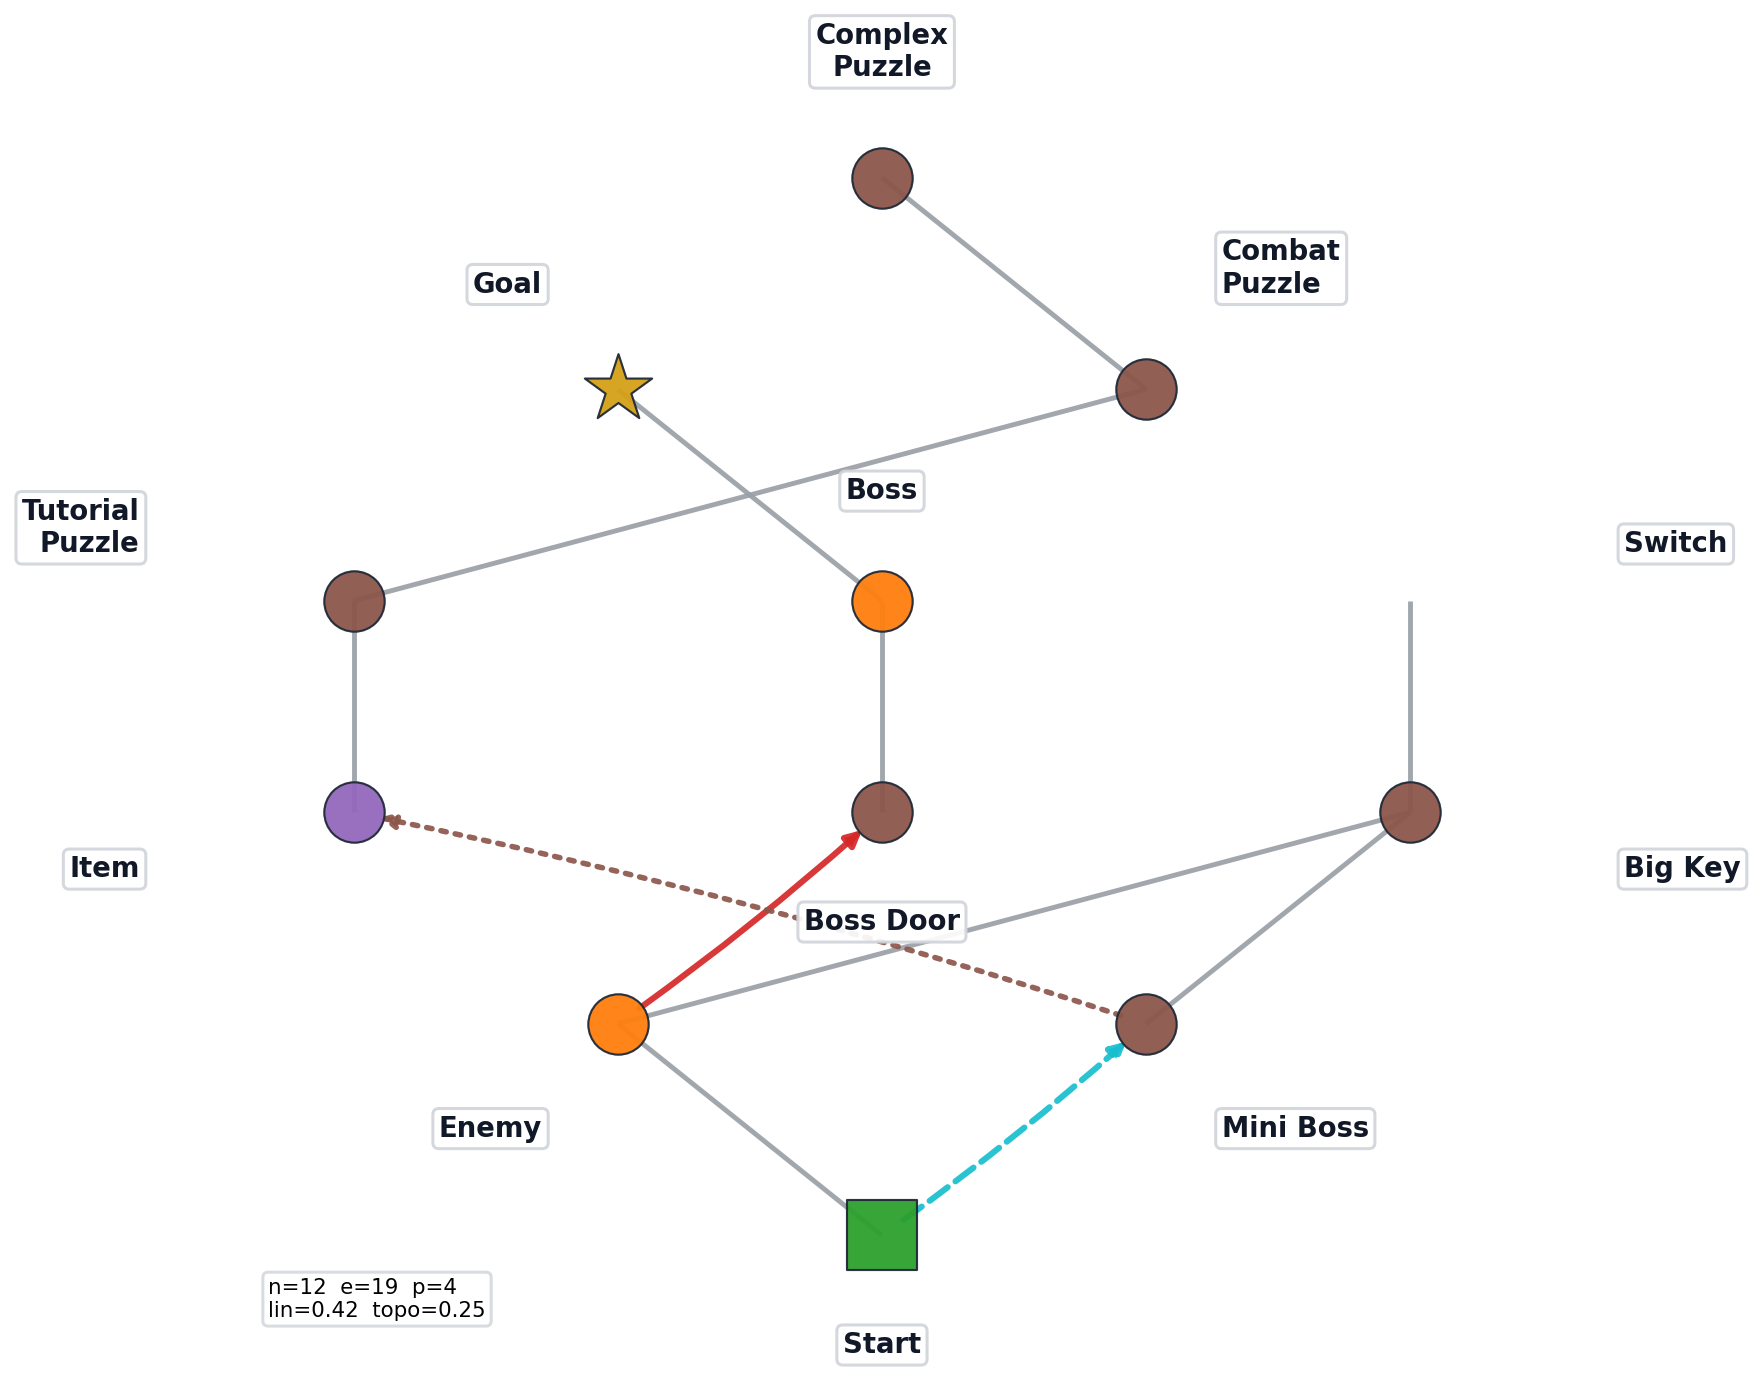
\includegraphics[width=\linewidth]{figures/ch4/generated_topology_seed20260418_graph.png}
\vspace{1mm}

{\scriptsize (a) Mission graph Block I sinh thật}
\end{minipage}
\hfill
\begin{minipage}[t]{0.52\linewidth}
\centering
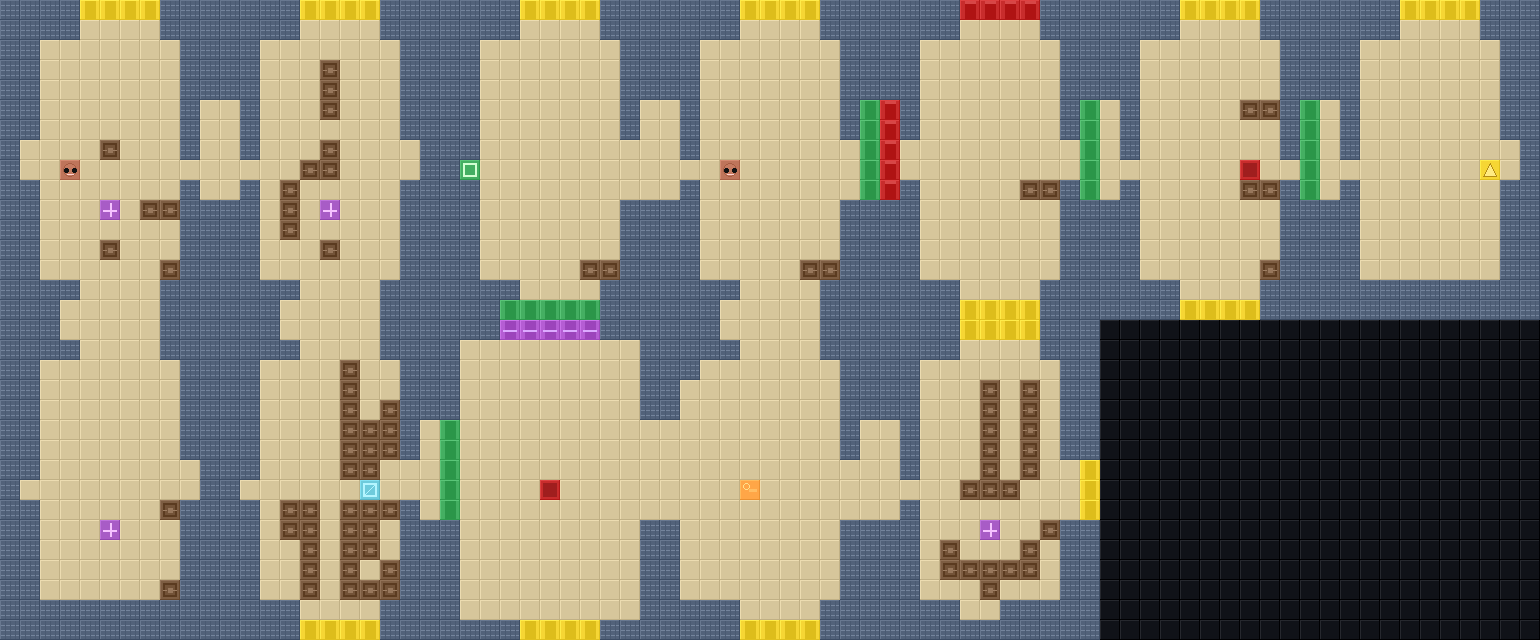
\includegraphics[width=\linewidth]{../results/ch4_generated_topology_real_pdrop035_seed20260418_fixedvalidator/diffusion_cfg3_logic0_steps50/dungeon_grid_stylized.png}
\vspace{1mm}

{\scriptsize (b) Dungeon đầu-cuối của nhánh khuếch tán chuẩn}
\end{minipage}
\caption{Một lượt chạy end-to-end thật của full pipeline: Block I sinh mission graph, ba nhánh sinh phòng dùng chung đồ thị đó, và dungeon ở hình (b) là mẫu khuếch tán được chọn để làm gốc cho bảng so sánh solver.}
\label{fig:real_generated_graph_and_best_dungeon}
\end{figure}

\begin{table}[H]
\centering
\small
\setlength{\tabcolsep}{4pt}
\renewcommand{\arraystretch}{1.08}
\caption{So sánh ba nhánh sinh phòng trên cùng đồ thị nhiệm vụ do Block I sinh thật}
\label{tab:overall_generated_graph_compare}
\resizebox{\textwidth}{!}{%
\begin{tabular}{@{}lcccccc@{}}
\toprule
Nhánh sinh phòng & Thời gian (s) $\downarrow$ & Tỉ lệ phòng phải sửa $\downarrow$ & Ghi đè marker $\downarrow$ & Hybrid contract & P-CBS & NCD gần tham chiếu $\downarrow$ \\
\midrule
Khuếch tán chuẩn & \textbf{21.46} & \textbf{0.917} & 0.167 & Đạt & Đạt & 0.623 \\
Lấy mẫu rút gọn & 68.26 & 1.000 & 0.167 & Đạt & Đạt & \textbf{0.607} \\
Sinh che khuất & 62.72 & 1.000 & \textbf{0.083} & Đạt & Đạt & 0.613 \\
\bottomrule
\end{tabular}%
}
\end{table}

Kết quả ở Bảng~\ref{tab:overall_generated_graph_compare} cho thấy cả ba nhánh đều đi hết chuỗi thẩm định khi dùng đồ thị nhiệm vụ sinh thật. Tuy nhiên, nhánh khuếch tán chuẩn vẫn là điểm vận hành cân bằng nhất vì nó giữ được toàn bộ hợp đồng cơ học--nhận thức với chi phí thấp hơn rõ rệt. Nhánh lấy mẫu rút gọn và nhánh che khuất có lợi ở một vài cột riêng lẻ như NCD hoặc tỉ lệ ghi đè marker, nhưng phần lợi đó không đủ bù cho thời gian đầu-cuối cao hơn gấp khoảng ba lần.

Để bảo đảm kết luận này không phụ thuộc vào một bộ giải duy nhất, khóa luận chạy đồng thời toàn bộ nhóm bộ giải tile-state độc lập có cùng mục tiêu START$\rightarrow$TRIFORCE trong repo, gồm A*, BFS, Dijkstra, Greedy, D* Lite, DFS/IDDFS và Bidirectional A*, rồi đối chiếu với P-CBS (balanced) trên chính dungeon khuếch tán ở Hình~\ref{fig:real_generated_graph_and_best_dungeon}. Các tiện ích \emph{parallel A*} và \emph{multi-goal search} không được đưa vào bảng chính vì một bên trùng mục tiêu với A* nhưng thêm phương sai do multiprocessing, còn một bên phục vụ routing nhiều mục tiêu thay vì bài toán một đích của giao thức validation.

\begin{table}[H]
\centering
\small
\setlength{\tabcolsep}{4pt}
\renewcommand{\arraystretch}{1.08}
\caption{So sánh bộ giải tìm kiếm trên dungeon khuếch tán sinh từ full pipeline thật}
\label{tab:search_solver_vs_pcbs}
\resizebox{\textwidth}{!}{%
\begin{tabular}{@{}lccccl@{}}
\toprule
Bộ giải & Giải được & Trạng thái $\downarrow$ & Thời gian (s) $\downarrow$ & Vai trò & Ghi chú \\
\midrule
A* & Không & 200000 & 14.69 & Hard oracle & Hết ngân sách tìm kiếm trên lưới ghép \\
BFS & Không & 50000 & 2.97 & Exact baseline & Hết ngân sách sau 50{,}000 trạng thái \\
Dijkstra & Không & 50000 & 4.03 & Exact baseline & Hết ngân sách sau 50{,}000 trạng thái \\
Greedy & Không & 50000 & 3.50 & Heuristic baseline & Mắc kẹt ở heuristic cục bộ \\
D* Lite & Không & 100000 & 7.68 & Incremental replanning & Rơi về fallback A* nhưng vẫn không hội tụ \\
DFS/IDDFS & Không & 103737 & 3.05 & Exhaustive probe & Mở rộng sâu nhưng không nối được tiến trình \\
Bidirectional A* & Có & 750 & \textbf{0.02} & Comparison search & Tìm được đường $84$ bước nhờ gặp frontier sớm \\
\midrule
P-CBS (balanced) & Có & \textbf{363} & -- & Behavioral probe & Thành công với confusion index $\approx 0.379$ \\
\bottomrule
\end{tabular}%
}
\end{table}

Bảng~\ref{tab:search_solver_vs_pcbs} cho thấy nhãn ``solvable'' phụ thuộc mạnh vào phương pháp đánh giá. Nếu chỉ nhìn hard A* thì mẫu này có vẻ chưa giải được vì bộ giải chạm trần trạng thái. Tuy nhiên, Bidirectional A* và P-CBS đều vượt qua trên cùng dungeon, còn graph-guided oracle và graph-progression cũng xác nhận tiến trình hợp lệ. Điều này không có nghĩa hard oracle trở nên thừa; ngược lại, nó cho thấy ba lớp đánh giá đang trả lời ba câu hỏi khác nhau: bộ solve cứng đo độ khó của không gian trạng thái đầy đủ, bộ solve đối xứng đo khả năng tìm đường khi đường kính hiệu dụng của lưới được giảm, còn P-CBS đo liệu một persona giới hạn thông tin có nối lại được lời giải hay không.

Một chẩn đoán phụ từ sweep puzzle profile cũng củng cố nhận định đó. Trên cấu hình ``không kiểm soát puzzle'', Greedy có thể tìm được lời giải sau $32{,}335$ trạng thái trong khi A*, BFS và Dijkstra vẫn timeout, còn P-CBS vẫn chấp nhận dungeon. Vì vậy, kết luận của Chương 4 không thể rút ra từ một solver duy nhất; mỗi phương pháp đánh giá nhấn mạnh một dạng ma sát khác nhau, từ độ nổ tổ hợp của tile-state cho đến mức rõ ràng của affordance tiến trình.

\section{Kết quả định lượng}
\subsection{Kết quả huấn luyện VQ-VAE nền tảng}
Sáu cấu hình VQ-VAE được huấn luyện trên cùng ngân sách 300 epoch để tách riêng ảnh hưởng của ba nhóm yếu tố: kích thước codebook, độ rộng hidden layer, và hai thành phần kiến trúc CoordConv/MRF. Khi đọc kết quả, cần phân biệt giữa hai khía cạnh: chất lượng hội tụ tại epoch tốt nhất và độ ổn định của mô hình về cuối quá trình huấn luyện. Bảng dưới đây tóm tắt các chỉ số này; với hai cột loss, giá trị càng thấp càng tốt, còn perplexity cao hơn cho thấy codebook được khai thác đa dạng hơn. Các giá trị tốt nhất theo từng cột được in đậm. Đồng thời, tất cả các run đều đạt codebook utilization 100\%, nên khác biệt quan sát được chủ yếu phản ánh năng lực tối ưu hóa chứ không phải hiện tượng collapse của latent.

\begin{table}[H]
\centering
\small
\setlength{\tabcolsep}{4pt}
\renewcommand{\arraystretch}{1.08}
\caption{So sánh sáu cấu hình VQ-VAE trên cùng lịch huấn luyện 300 epoch}
\label{tab:vqvae_ablation_results}
\resizebox{\textwidth}{!}{%
\begin{tabular}{@{}lccccc@{}}
\toprule
Cấu hình & Epoch tốt nhất & Val loss tốt nhất & Val loss cuối & Perplexity tốt nhất & Sử dụng codebook \\
\midrule
Cơ sở & 294 & \textbf{6.93e-5} & \textbf{1.05e-4} & 40.48 & 100\% \\
Codebook 128 & 161 & 8.82e-5 & 6.90e-4 & 35.89 & 100\% \\
Codebook 512 & 241 & 2.52e-3 & 5.63e-3 & \textbf{42.34} & 100\% \\
Hidden 64 & 119 & 7.47e-5 & 1.26e-4 & 40.79 & 100\% \\
Bỏ CoordConv & 203 & 3.19e-3 & 6.14e-3 & 39.95 & 100\% \\
Bỏ MRF & 187 & 2.34e-4 & 5.08e-3 & 40.57 & 100\% \\
\bottomrule
\end{tabular}%
}
\end{table}

Kết quả cho thấy cấu hình cơ sở là cấu hình cân bằng nhất: vừa đạt val loss thấp nhất, vừa giữ khoảng cách giữa giá trị tốt nhất và giá trị cuối ở mức nhỏ, nên quá trình hội tụ ổn định hơn so với các biến thể loại trừ. Hai biến thể hidden 64 và codebook 128 có chất lượng khá gần cấu hình cơ sở nhưng không tạo ra cải thiện rõ rệt. Ngược lại, codebook 512 và đặc biệt là việc bỏ CoordConv làm chất lượng hội tụ giảm đáng kể; bỏ MRF cũng làm val loss cuối tăng lên rõ rệt, dù giá trị tốt nhất vẫn còn chấp nhận được. Từ góc nhìn này, CoordConv và MRF là hai thành phần có đóng góp rõ ràng nhất cho độ ổn định của tiền huấn luyện.

\subsection{Kết quả tổng thể so với các cấu hình đối chứng}
Sau khi đã xác nhận full pipeline hoạt động được trên đồ thị sinh thật, khóa luận quay lại thiết kế đối chứng có kiểm soát trên một đồ thị nhiệm vụ cố định $12$ phòng, cùng seed và cùng tầng hậu xử lý, nhằm tách riêng ảnh hưởng của nhánh sinh phòng. Bảng~\ref{tab:overall_branch_compare} vì vậy không nhằm thay thế kết quả end-to-end ở Mục 4.2, mà dùng để đọc đóng góp biên trong điều kiện nhiễu cấu trúc đã được khóa lại. Trên thiết kế này, nhánh khuếch tán chuẩn vẫn là cấu hình cân bằng nhất: đây là nhánh nhanh nhất ở mức toàn chuỗi, vẫn vượt qua bộ kiểm tra cơ học và đồng thời được P-CBS chấp nhận. Nhánh lấy mẫu rút gọn giảm tỉ lệ can thiệp hậu kỳ so với khuếch tán chuẩn, nhưng lại chậm hơn rất nhiều khi tính cả sửa lỗi và phủ lại dấu mốc. Nhánh sinh che khuất tạo ra dungeon gần mẫu tham chiếu nhất theo NCD, song không vượt qua được tầng thẩm định nhận thức trong đúng kịch bản cố định này.

\begin{table}[H]
\centering
\small
\setlength{\tabcolsep}{4pt}
\renewcommand{\arraystretch}{1.08}
\caption{So sánh ba nhánh sinh phòng trên cùng một đồ thị nhiệm vụ cố định}
\label{tab:overall_branch_compare}
\resizebox{\textwidth}{!}{%
\begin{tabular}{@{}lccccc@{}}
\toprule
Nhánh sinh phòng & Thời gian (s) $\downarrow$ & Tỉ lệ phòng phải sửa $\downarrow$ & Ghi đè marker $\downarrow$ & P-CBS & NCD gần tham chiếu $\downarrow$ \\
\midrule
Khuếch tán chuẩn & \textbf{47.84} & 1.000 & 0.292 & Đạt & 0.608 \\
Lấy mẫu rút gọn & 100.80 & 0.833 & \textbf{0.167} & Đạt & 0.628 \\
Sinh che khuất & 49.52 & \textbf{0.667} & \textbf{0.167} & Không đạt & \textbf{0.568} \\
\bottomrule
\end{tabular}%
}
\end{table}

Điểm đáng chú ý ở đây là thời gian của nhánh lấy mẫu rút gọn không còn phản ánh riêng số bước sinh. Khi cộng cả chi phí sửa tile, vá ràng buộc hình học, phủ marker và hậu kiểm, nhánh này chậm hơn khuếch tán chuẩn hơn gấp đôi. Do đó, nếu mục tiêu là sinh dungeon hoàn chỉnh chứ không chỉ rút ngắn pha lấy mẫu, nhánh khuếch tán chuẩn vẫn là lựa chọn hợp lý hơn.

\begin{figure}[H]
\centering
\begin{minipage}[t]{0.32\linewidth}
\centering
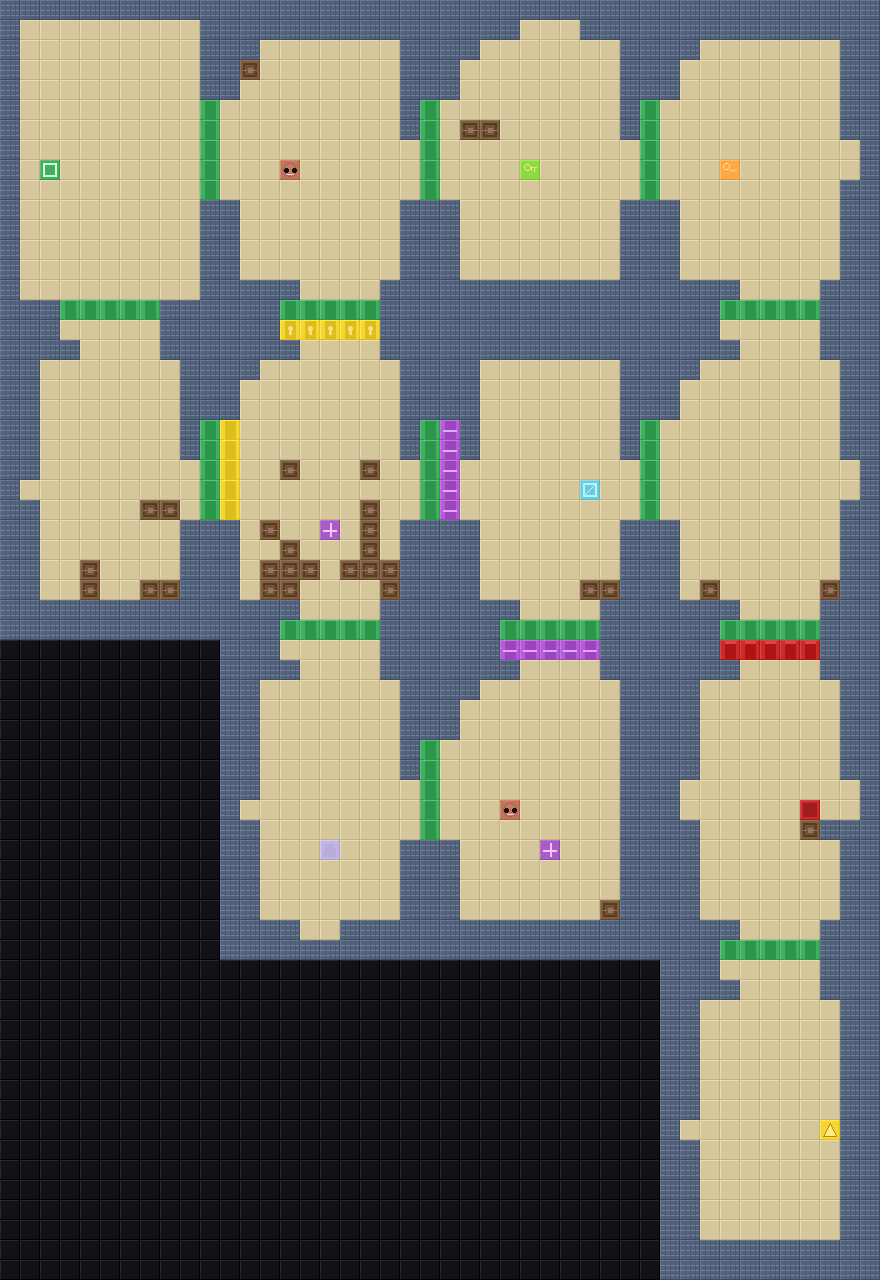
\includegraphics[width=\linewidth]{../results/thesis_ch4_evals/branch_compare_pdrop035/pdrop035/diffusion_cfg3_logic0_steps50/dungeon_grid_stylized.png}
\vspace{1mm}

{\scriptsize (a) Khuếch tán chuẩn}
\end{minipage}
\hfill
\begin{minipage}[t]{0.32\linewidth}
\centering
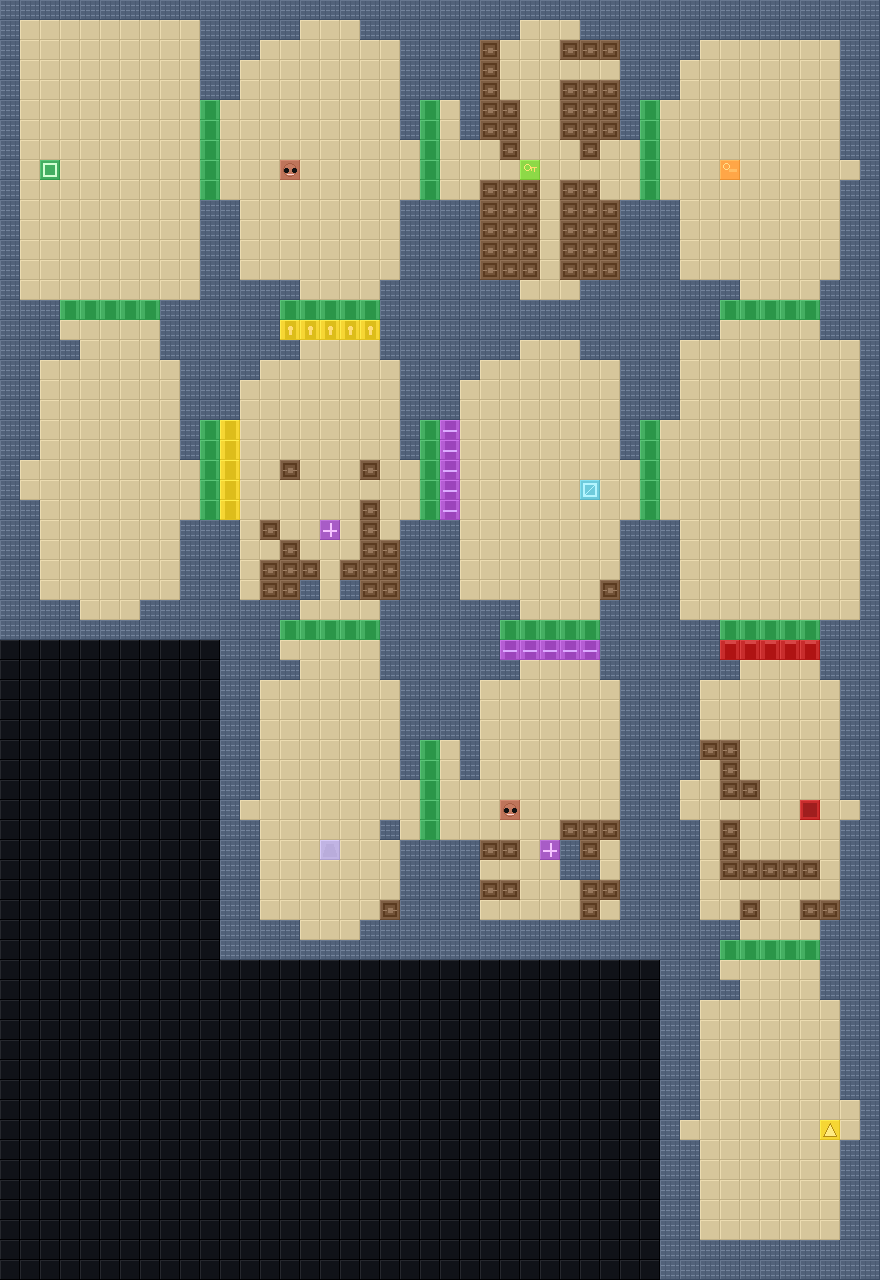
\includegraphics[width=\linewidth]{../results/thesis_ch4_evals/branch_compare_pdrop035/pdrop035/fast_cfg3_logic0_steps4/dungeon_grid_stylized.png}
\vspace{1mm}

{\scriptsize (b) Lấy mẫu rút gọn}
\end{minipage}
\hfill
\begin{minipage}[t]{0.32\linewidth}
\centering
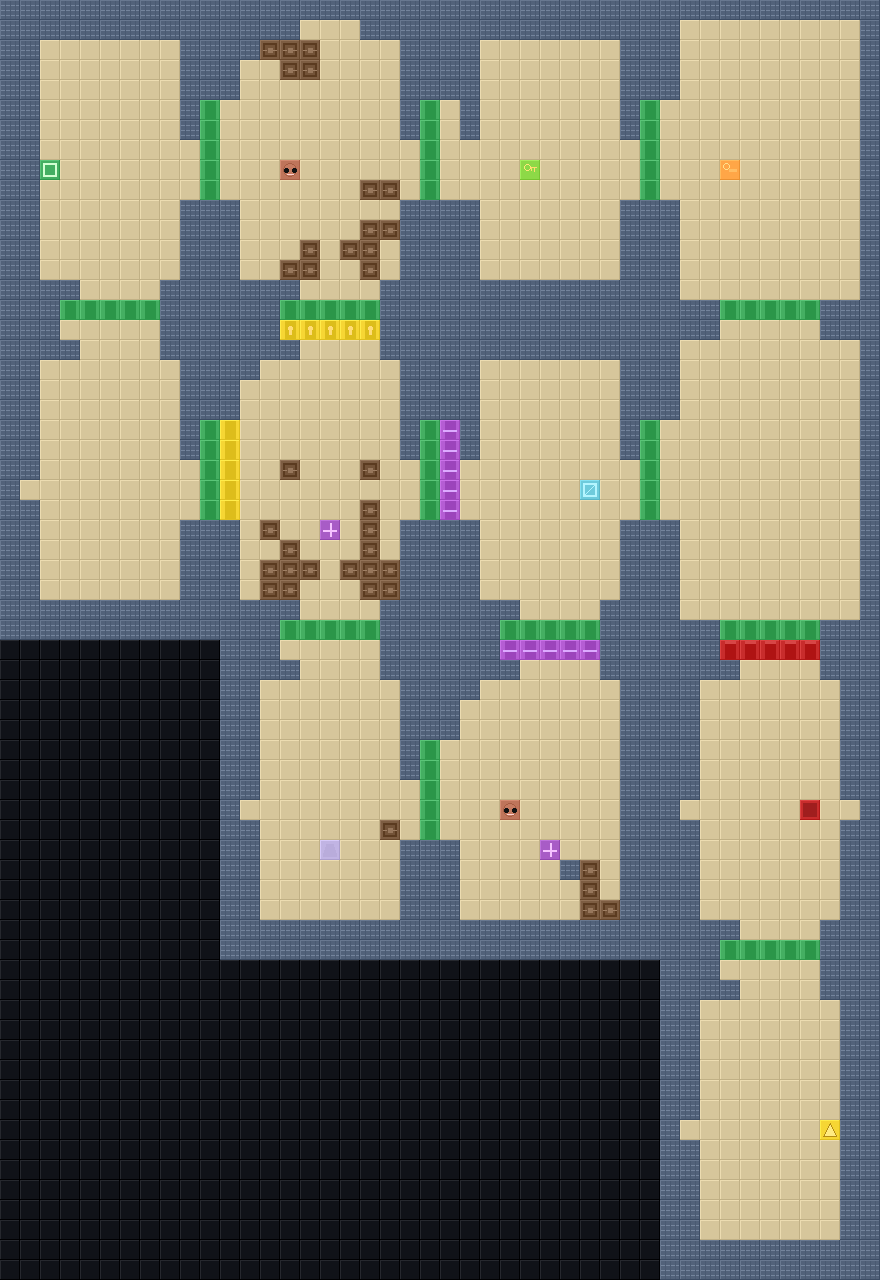
\includegraphics[width=\linewidth]{../results/thesis_ch4_evals/branch_compare_pdrop035/pdrop035/masked_room_full/dungeon_grid_stylized.png}
\vspace{1mm}

{\scriptsize (c) Sinh che khuất}
\end{minipage}
\caption{Ba dungeon sinh ra từ cùng một đồ thị nhiệm vụ. Nhánh khuếch tán chuẩn giữ được thế cân bằng tốt hơn giữa độ sạch cơ học, chi phí và khả năng được tầng thẩm định nhận thức chấp nhận.}
\label{fig:branch_visual_examples}
\end{figure}

\subsection{Kết quả loại trừ theo từng khối của quy trình}
Các ablation được đọc theo logic thành phần: trước hết là cường độ bỏ điều kiện ngẫu nhiên trong huấn luyện, sau đó là bộ mã lượng tử ở tầng nén phòng, rồi đến các tín hiệu điều khiển ngữ nghĩa và cấu trúc. Bảng~\ref{tab:pdrop_sweep_results} cho thấy ba mức bỏ điều kiện tạo ra một đánh đổi rõ. Mức $0.15$ cần ít can thiệp hậu kỳ nhất, trong khi mức $0.35$ cho dungeon gần dữ liệu tham chiếu hơn và đồng thời nhanh nhất ở mức toàn chuỗi. Mức $0.55$ không tạo được cải thiện thêm về độ gần tham chiếu, nhưng vẫn làm tăng số tile phải sửa.

\begin{table}[H]
\centering
\small
\setlength{\tabcolsep}{4pt}
\renewcommand{\arraystretch}{1.08}
\caption{Ảnh hưởng của xác suất bỏ điều kiện trong nhánh khuếch tán}
\label{tab:pdrop_sweep_results}
\begin{tabular}{@{}lcccc@{}}
\toprule
Mức bỏ điều kiện & Thời gian (s) $\downarrow$ & Tỉ lệ phòng phải sửa $\downarrow$ & Ghi đè marker $\downarrow$ & NCD gần tham chiếu $\downarrow$ \\
\midrule
$0.15$ & 47.54 & \textbf{0.917} & \textbf{0.250} & 0.616 \\
$0.35$ & \textbf{46.49} & 1.000 & 0.292 & \textbf{0.603} \\
$0.55$ & 47.88 & 1.000 & 0.292 & 0.617 \\
\bottomrule
\end{tabular}
\end{table}

Trên tầng mã lượng tử, việc tăng kích thước codebook từ $256$ lên $512$ chỉ thực sự có ích cho nhánh khuếch tán. Ở nhánh này, thời gian giảm từ $38.74$ xuống \textbf{$37.82$} giây, NCD gần tham chiếu giảm từ $0.631$ xuống \textbf{$0.608$}, đồng thời vẫn được P-CBS chấp nhận. Trái lại, với nhánh sinh che khuất, codebook $512$ làm giảm ghi đè marker xuống \textbf{$0.083$} nhưng lại khiến P-CBS không chấp nhận và tăng thời gian lên $53.16$ giây. Bảng~\ref{tab:tokenizer_compare_results} tóm tắt hiện tượng này.

\begin{table}[H]
\centering
\small
\setlength{\tabcolsep}{4pt}
\renewcommand{\arraystretch}{1.08}
\caption{So sánh hai kích thước codebook trên hai nhánh sinh phòng}
\label{tab:tokenizer_compare_results}
\resizebox{\textwidth}{!}{%
\begin{tabular}{@{}lccccc@{}}
\toprule
Nhánh / codebook & Thời gian (s) $\downarrow$ & Tỉ lệ phòng phải sửa $\downarrow$ & Ghi đè marker $\downarrow$ & P-CBS & NCD gần tham chiếu $\downarrow$ \\
\midrule
Khuếch tán / 256 & 38.74 & 0.833 & 0.250 & Đạt & 0.631 \\
Khuếch tán / 512 & \textbf{37.82} & 1.000 & 0.250 & Đạt & 0.608 \\
Che khuất / 256 & 49.77 & 0.667 & 0.250 & Đạt & \textbf{0.579} \\
Che khuất / 512 & 53.16 & \textbf{0.583} & \textbf{0.083} & Không đạt & 0.590 \\
\bottomrule
\end{tabular}%
}
\end{table}

\begin{figure}[H]
\centering
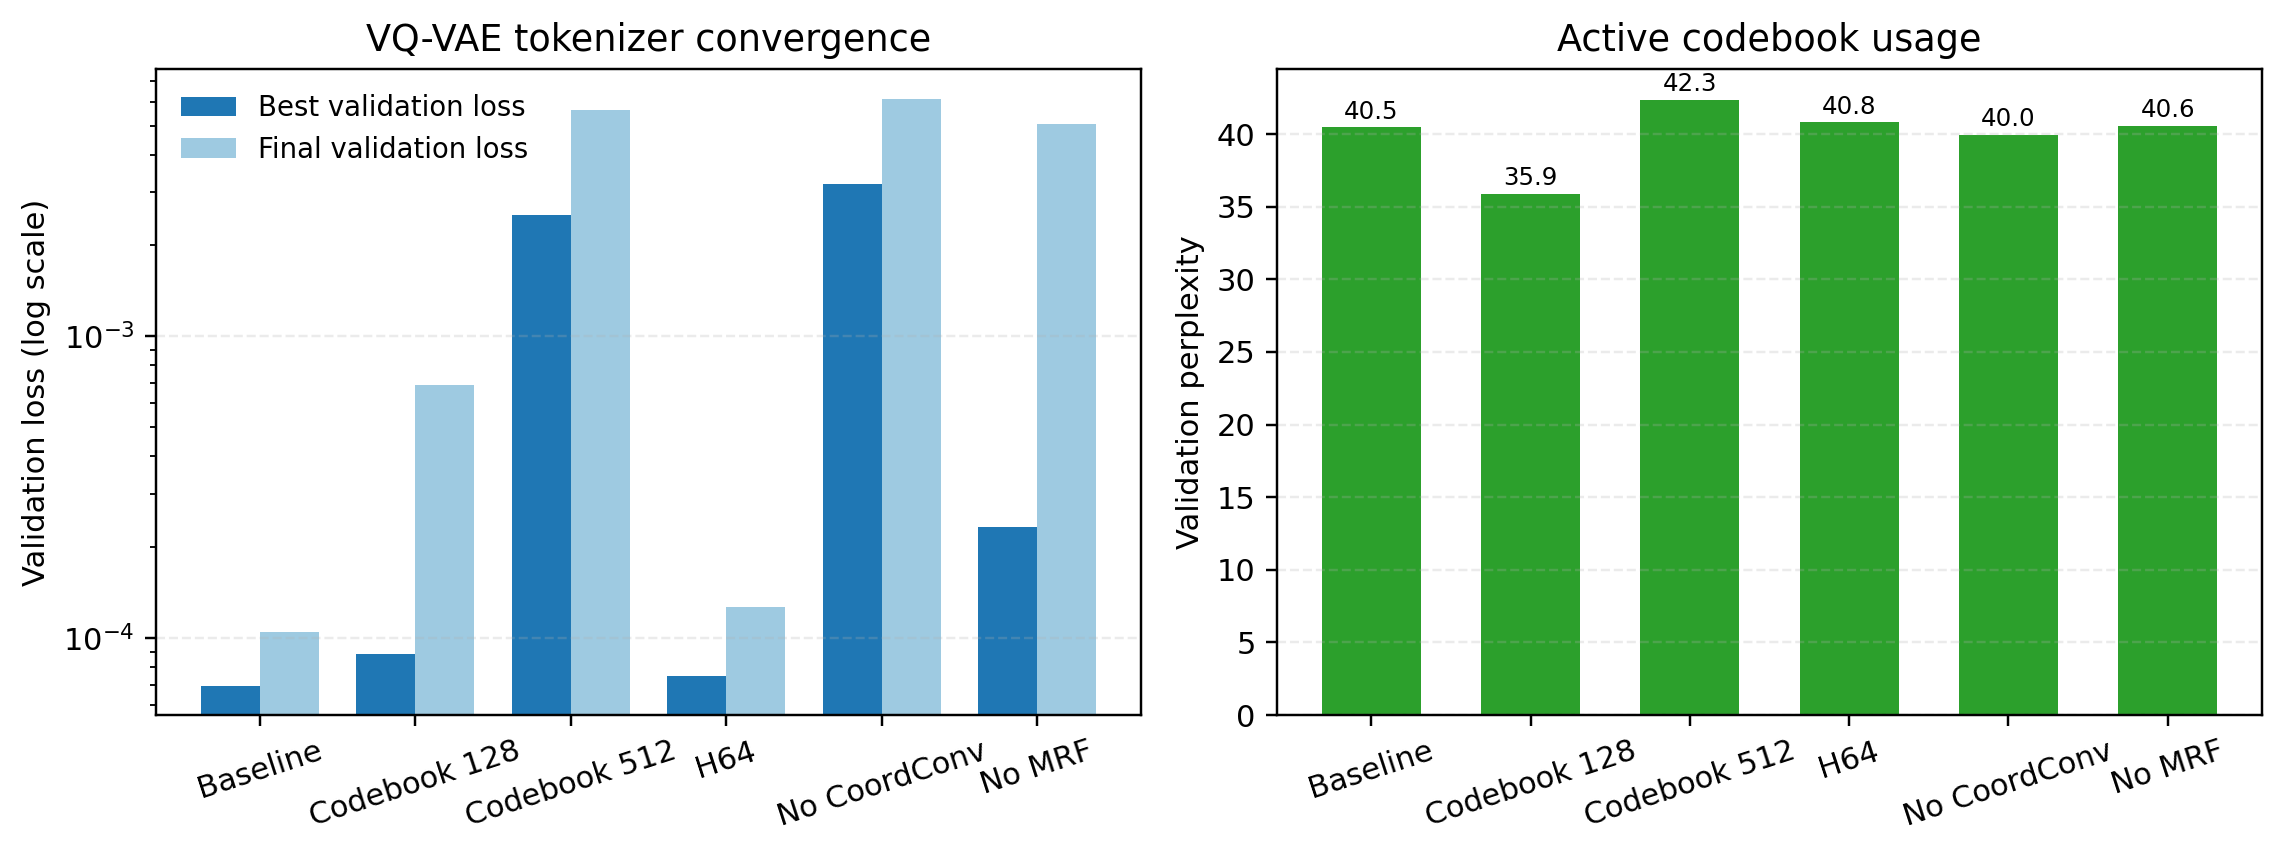
\includegraphics[width=0.96\linewidth]{figures/ch4/vqvae_ablation_overview.png}
\caption{Tổng quan hội tụ của các biến thể tokenizer VQ-VAE. Biểu đồ trái so sánh validation loss tốt nhất và ở cuối quá trình huấn luyện; biểu đồ phải cho thấy độ rộng codebook được khai thác qua validation perplexity.}
\label{fig:vqvae_ablation_overview}
\end{figure}

Hình~\ref{fig:vqvae_ablation_overview} bổ sung bằng chứng ở tầng nén phòng cho nhận xét trong Bảng~\ref{tab:tokenizer_compare_results}. Cấu hình nền đạt validation loss thấp nhất, còn biến thể codebook $512$ duy trì validation perplexity cao nhất, tức sử dụng được dải mã lượng tử rộng hơn nhưng phải trả giá bằng động học hội tụ khó hơn. Điều này giải thích vì sao codebook lớn chỉ thực sự có lợi khi đi cùng nhánh khuếch tán và tín hiệu điều kiện đủ ổn định: ở bối cảnh đó, lợi ích từ không gian mã phong phú hơn còn vượt được chi phí học thêm, trong khi ở nhánh che khuất, cùng một mức mở rộng codebook lại dễ làm tăng sai lệch ở tầng hậu thẩm định.

Hai nhóm tín hiệu điều khiển ở tầng cao hơn cũng để lại dấu vết rõ trên kết quả. Khi tăng cường ngữ nghĩa theo giai đoạn, nhánh khuếch tán nâng được tỉ lệ qua bộ kiểm tra cơ học từ $0.833$ lên $0.917$, nhưng đồng thời đánh mất chấp nhận của P-CBS và tăng thời gian từ $38.25$ lên $47.65$ giây. Với điều khiển cấu trúc, hiệu ứng lại tích cực hơn: thời gian giảm mạnh từ $83.61$ xuống $38.36$ giây, NCD gần tham chiếu giảm từ $0.613$ xuống $0.605$, và tỉ lệ phòng phải sửa cũng giảm từ $1.000$ xuống $0.917$. Nói cách khác, tín hiệu cấu trúc đang phát huy vai trò ổn định hóa rõ hơn so với việc chỉ tăng thêm nhãn ngữ nghĩa cục bộ.

\begin{figure}[H]
\centering
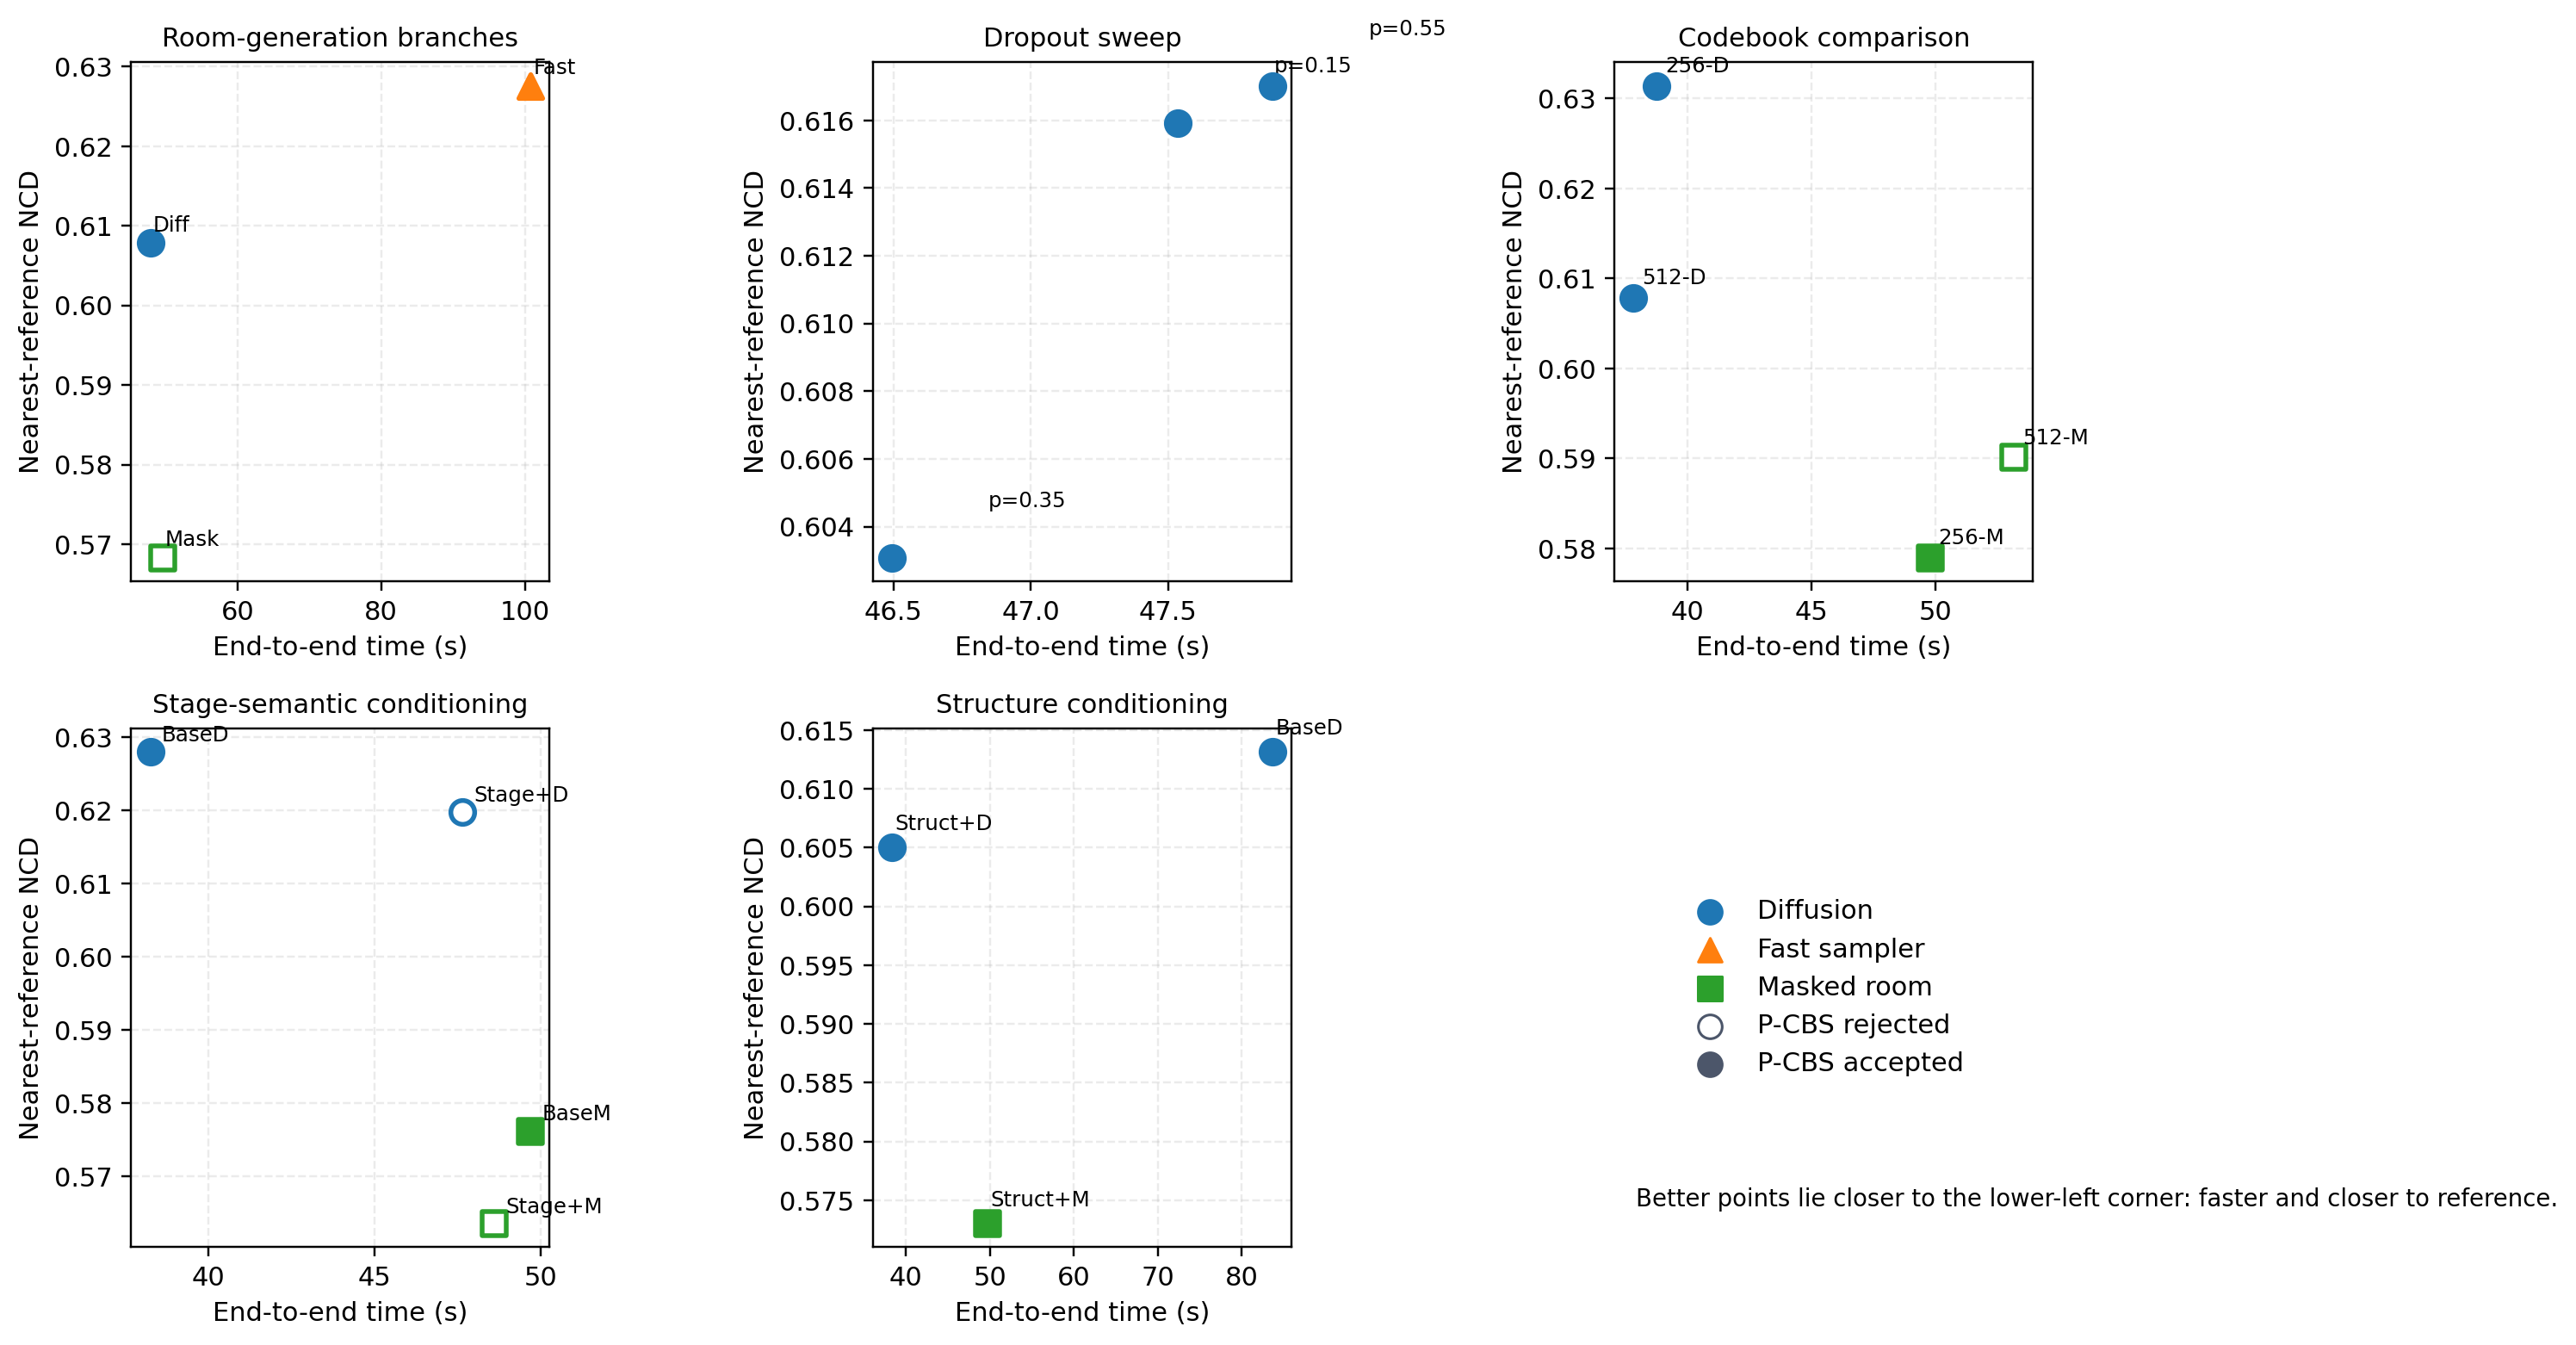
\includegraphics[width=0.98\linewidth]{figures/ch4/room_generation_landscape.png}
\caption{Cảnh quan đánh đổi giữa chi phí và độ gần tham chiếu của các ablation ở tầng sinh phòng. Mỗi điểm biểu diễn một cấu hình; các điểm được P-CBS chấp nhận được tô đặc, còn các điểm bị bác bỏ được để rỗng.}
\label{fig:room_generation_landscape}
\end{figure}

Quan sát tổng hợp ở Hình~\ref{fig:room_generation_landscape} cho thấy vùng hiệu quả nhất tập trung quanh các cấu hình khuếch tán có $p_{\text{drop}}=0.35$ và biến thể khuếch tán có điều khiển cấu trúc, vì chúng nằm gần góc trái dưới hơn hầu hết các điểm còn lại. Nhóm che khuất có thể kéo NCD xuống thấp hơn trong một số cấu hình, nhưng cụm điểm của nó phân tán hơn về thời gian và trạng thái chấp nhận của P-CBS. Trong khi đó, nhánh lấy mẫu nhanh chủ yếu dịch sang hướng chi phí cao hơn hoặc NCD kém hơn, cho thấy lợi ích thời gian của nó không bù được phần suy giảm ổn định khi xét ở mức toàn chuỗi.

\subsection{Độ nhạy của tầng thẩm định nhận thức}
Để đọc rõ vai trò của từng thành phần trong P-CBS, khóa luận dùng một bộ kiểm thử thành phần trên sáu bản đồ thuộc ba dungeon đầu với hồ sơ người chơi cân bằng. Bảng~\ref{tab:pcbs_ablation_results} cho thấy hai thành phần khó bỏ nhất là cơ chế quay lại có kiểm soát và mô hình hóa bất định. Khi loại bỏ một trong hai, tỉ lệ thành công giảm từ $33.3\%$ xuống còn $16.7\%$, trong khi chỉ số rối trí tăng mạnh. Ngược lại, việc tắt cơ chế tập trung làm giảm chỉ số rối trí trên bộ nhỏ này, nhưng không tạo được cải thiện về tỉ lệ thành công so với cấu hình đầy đủ.

\begin{table}[H]
\centering
\small
\setlength{\tabcolsep}{4pt}
\renewcommand{\arraystretch}{1.08}
\caption{Độ nhạy của P-CBS theo từng nhóm thành phần trên hồ sơ người chơi cân bằng}
\label{tab:pcbs_ablation_results}
\begin{tabular}{@{}lccc@{}}
\toprule
Biến thể & Thành công (\%) $\uparrow$ & Chỉ số rối trí $\downarrow$ & Mức bức bối cực đại $\downarrow$ \\
\midrule
Đầy đủ & \textbf{33.3} & 51.761 & 0.976 \\
Bỏ quay lại có kiểm soát & 16.7 & 73.802 & 1.106 \\
Bỏ mô hình bất định & 16.7 & 70.476 & 1.064 \\
Bỏ cơ chế tập trung & \textbf{33.3} & \textbf{39.920} & \textbf{0.836} \\
\bottomrule
\end{tabular}
\end{table}

Kết quả này cần được đọc theo đúng phạm vi của nó. Trên bộ bản đồ nhỏ, một số thành phần có thể làm giảm ma sát nhận thức cục bộ khi bị tắt đi; tuy nhiên, hai cơ chế quay lại có kiểm soát và mô hình hóa bất định lại là nền tảng để tránh sụt giảm mạnh tỉ lệ thành công. Vì vậy, tầng thẩm định nhận thức không chỉ là một lớp chấm điểm hậu kỳ mà còn là nơi bộc lộ trực tiếp giá trị của các giả định về hành vi người chơi.

\begin{figure}[H]
\centering
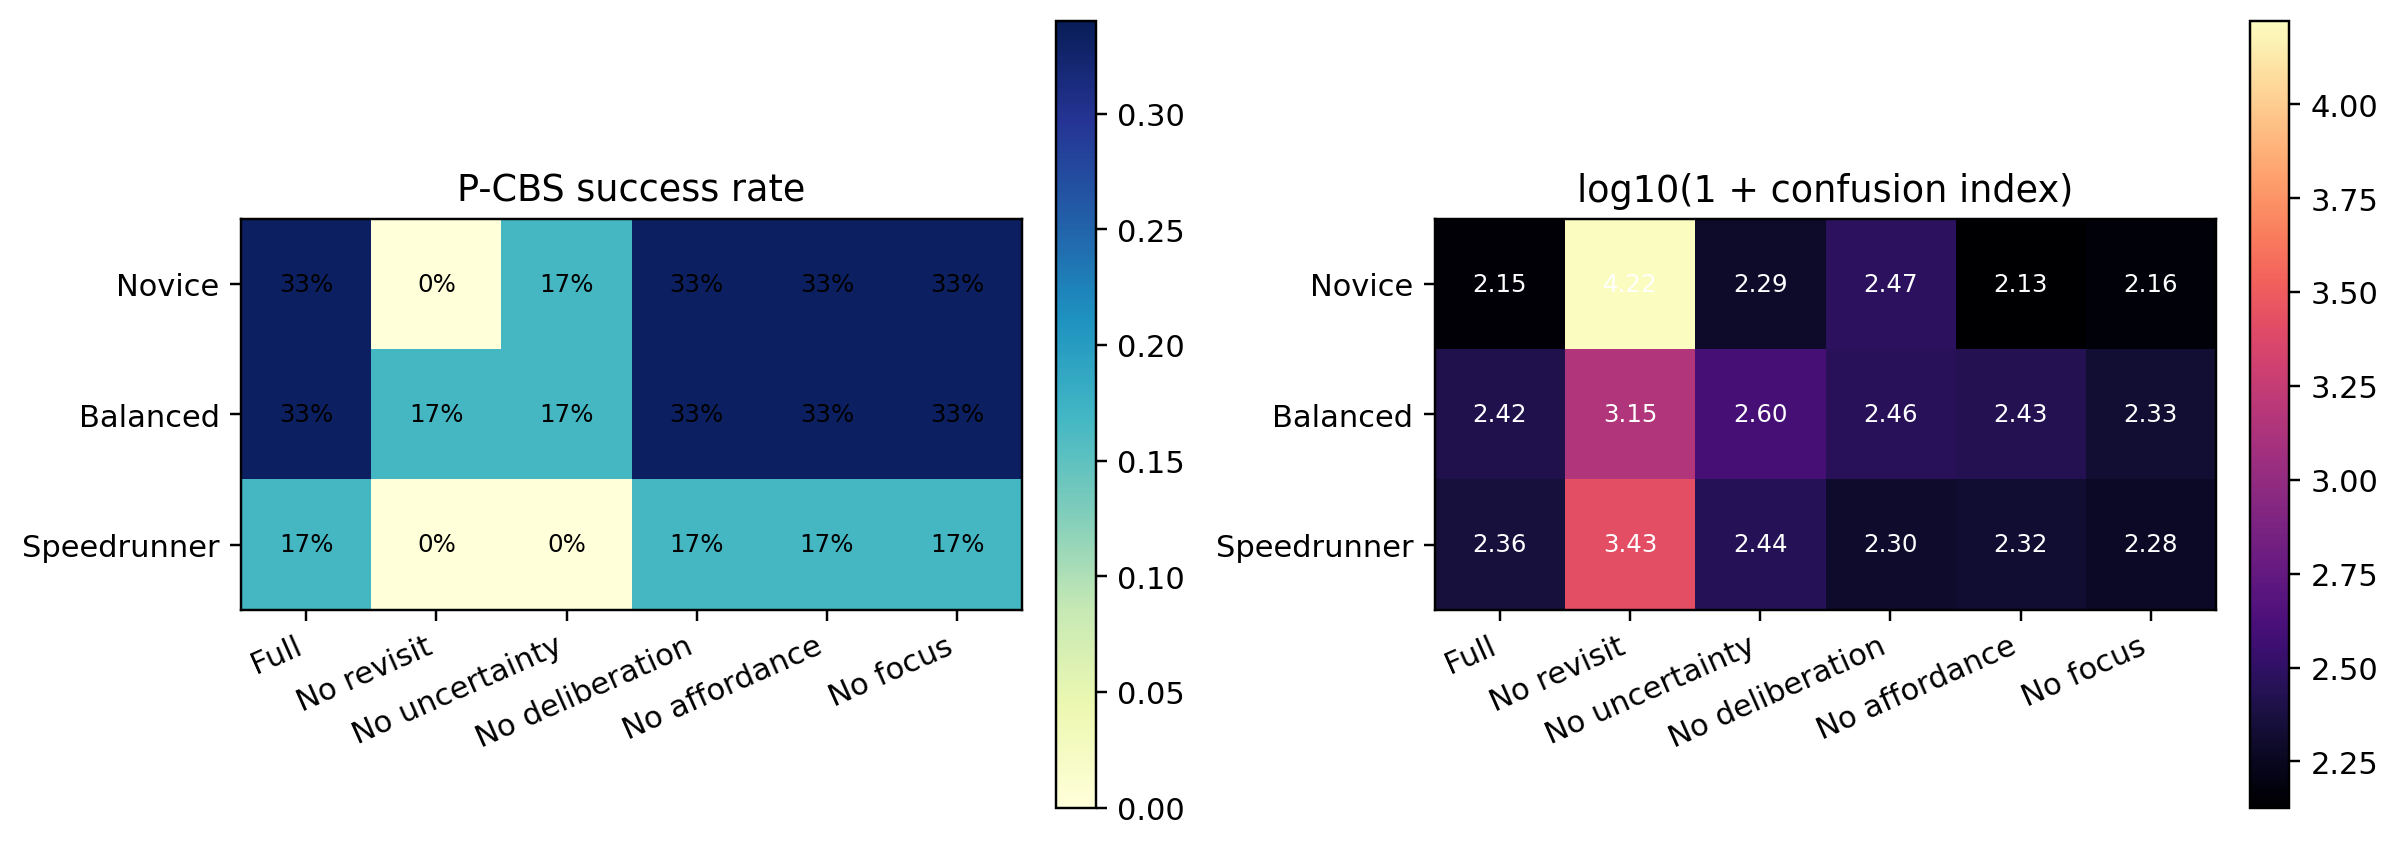
\includegraphics[width=0.98\linewidth]{figures/ch4/pcbs_persona_ablation_heatmap.png}
\caption{Tổng hợp ablation P-CBS trên hai hồ sơ persona đã hoàn tất đầy đủ. Biểu đồ trái cho thấy tỉ lệ thành công; biểu đồ phải biểu diễn chỉ số rối trí sau biến đổi $\log_{10}(1+x)$ để các biến thể có thể được đọc trên cùng một thang màu.}
\label{fig:pcbs_persona_ablation_heatmap}
\end{figure}

Hình~\ref{fig:pcbs_persona_ablation_heatmap} mở rộng kết luận ở trên từ một hồ sơ \emph{balanced} sang hai hồ sơ persona đã có đủ nhật ký thành phần. Xu hướng ổn định nhất giữa hai hồ sơ là vai trò thiết yếu của cơ chế quay lại có kiểm soát và mô hình hóa bất định: khi bỏ \emph{revisit}, tỉ lệ thành công giảm từ $33.3\%$ xuống $0\%$ ở novice và xuống $16.7\%$ ở balanced, đồng thời chỉ số rối trí tăng vọt; khi bỏ \emph{uncertainty}, cả hai hồ sơ đều chỉ còn $16.7\%$ thành công. Ngược lại, việc bỏ \emph{affordance}, \emph{deliberation} hoặc \emph{focus} chưa làm tỉ lệ thành công giảm ngay trên bộ nhỏ này, nhưng vẫn làm thay đổi chi phí nhận thức theo những hướng khác nhau giữa hai persona. Vì vậy, nếu đọc P-CBS như một mô hình nhận thức phân tầng, \emph{revisit} và \emph{uncertainty} là hai cơ chế lõi giữ được tính bền vững xuyên persona, còn các cơ chế còn lại chủ yếu điều biến mức ma sát nhận thức thay vì quyết định trực tiếp khả năng vượt ải.

\subsection{Kết quả so sánh đồng ngân sách ở tầng đồ thị nhiệm vụ}
Ở tầng đồ thị nhiệm vụ, thí nghiệm đồng ngân sách được chạy với cùng mức đánh giá $512$ lần cho mỗi phương pháp. Bảng~\ref{tab:matched_budget_results} cho thấy chiến lược tiến hóa thuần đạt điểm thích nghi trung bình cao nhất, trong khi cấu hình đầy đủ không dẫn đầu ở thước đo này. Tuy nhiên, cấu hình đầy đủ lại sinh ra đồ thị giàu cấu trúc hơn: số nút trung bình cao nhất và số thành phần bí mật cũng cao nhất. Điều đó cho thấy lợi ích của cấu hình đầy đủ nằm ở độ phong phú ngữ nghĩa của đồ thị, chứ không chỉ ở một thước đo tổng hợp đơn lẻ.

\begin{table}[H]
\centering
\small
\setlength{\tabcolsep}{4pt}
\renewcommand{\arraystretch}{1.08}
\caption{So sánh đồng ngân sách ở tầng đồ thị nhiệm vụ}
\label{tab:matched_budget_results}
\resizebox{\textwidth}{!}{%
\begin{tabular}{@{}lccccc@{}}
\toprule
Phương pháp & Điểm thích nghi $\uparrow$ & Hợp lệ vận hành $\uparrow$ & Số nút TB $\uparrow$ & Thành phần bí mật TB $\uparrow$ & Thời gian (s) $\downarrow$ \\
\midrule
Ngẫu nhiên & 0.192 & 0.812 & 15.61 & 0.406 & \textbf{7.75} \\
Tiến hóa chiến lược & \textbf{0.317} & \textbf{1.000} & 25.70 & 0.406 & 12.27 \\
Di truyền & 0.302 & \textbf{1.000} & 27.20 & 0.406 & 12.54 \\
MAP-Elites & 0.283 & \textbf{1.000} & 27.25 & 0.281 & 10.50 \\
Đầy đủ & 0.293 & 0.984 & \textbf{28.30} & \textbf{0.547} & 12.79 \\
\bottomrule
\end{tabular}%
}
\end{table}

Vì vậy, nếu mục tiêu là tối đa hóa fitness dưới một ngân sách ngắn, chiến lược tiến hóa thuần đang có lợi thế. Ngược lại, nếu muốn giữ được đồ thị nhiệm vụ phong phú hơn về tiến trình, phân nhánh và nội dung bí mật để cấp cho tầng sinh phòng, cấu hình đầy đủ vẫn là lựa chọn đáng giá dù chi phí cao hơn đôi chút. Để trực quan hóa topology bằng dữ liệu sinh thật thay vì hình vẽ thủ công, Hình~\ref{fig:block_i_mission_graph_layout} trình bày trực tiếp các đồ thị do Block I sinh ra từ pipeline đánh giá.

\begin{figure}[H]
\centering
\begin{subfigure}[t]{0.96\linewidth}
\centering
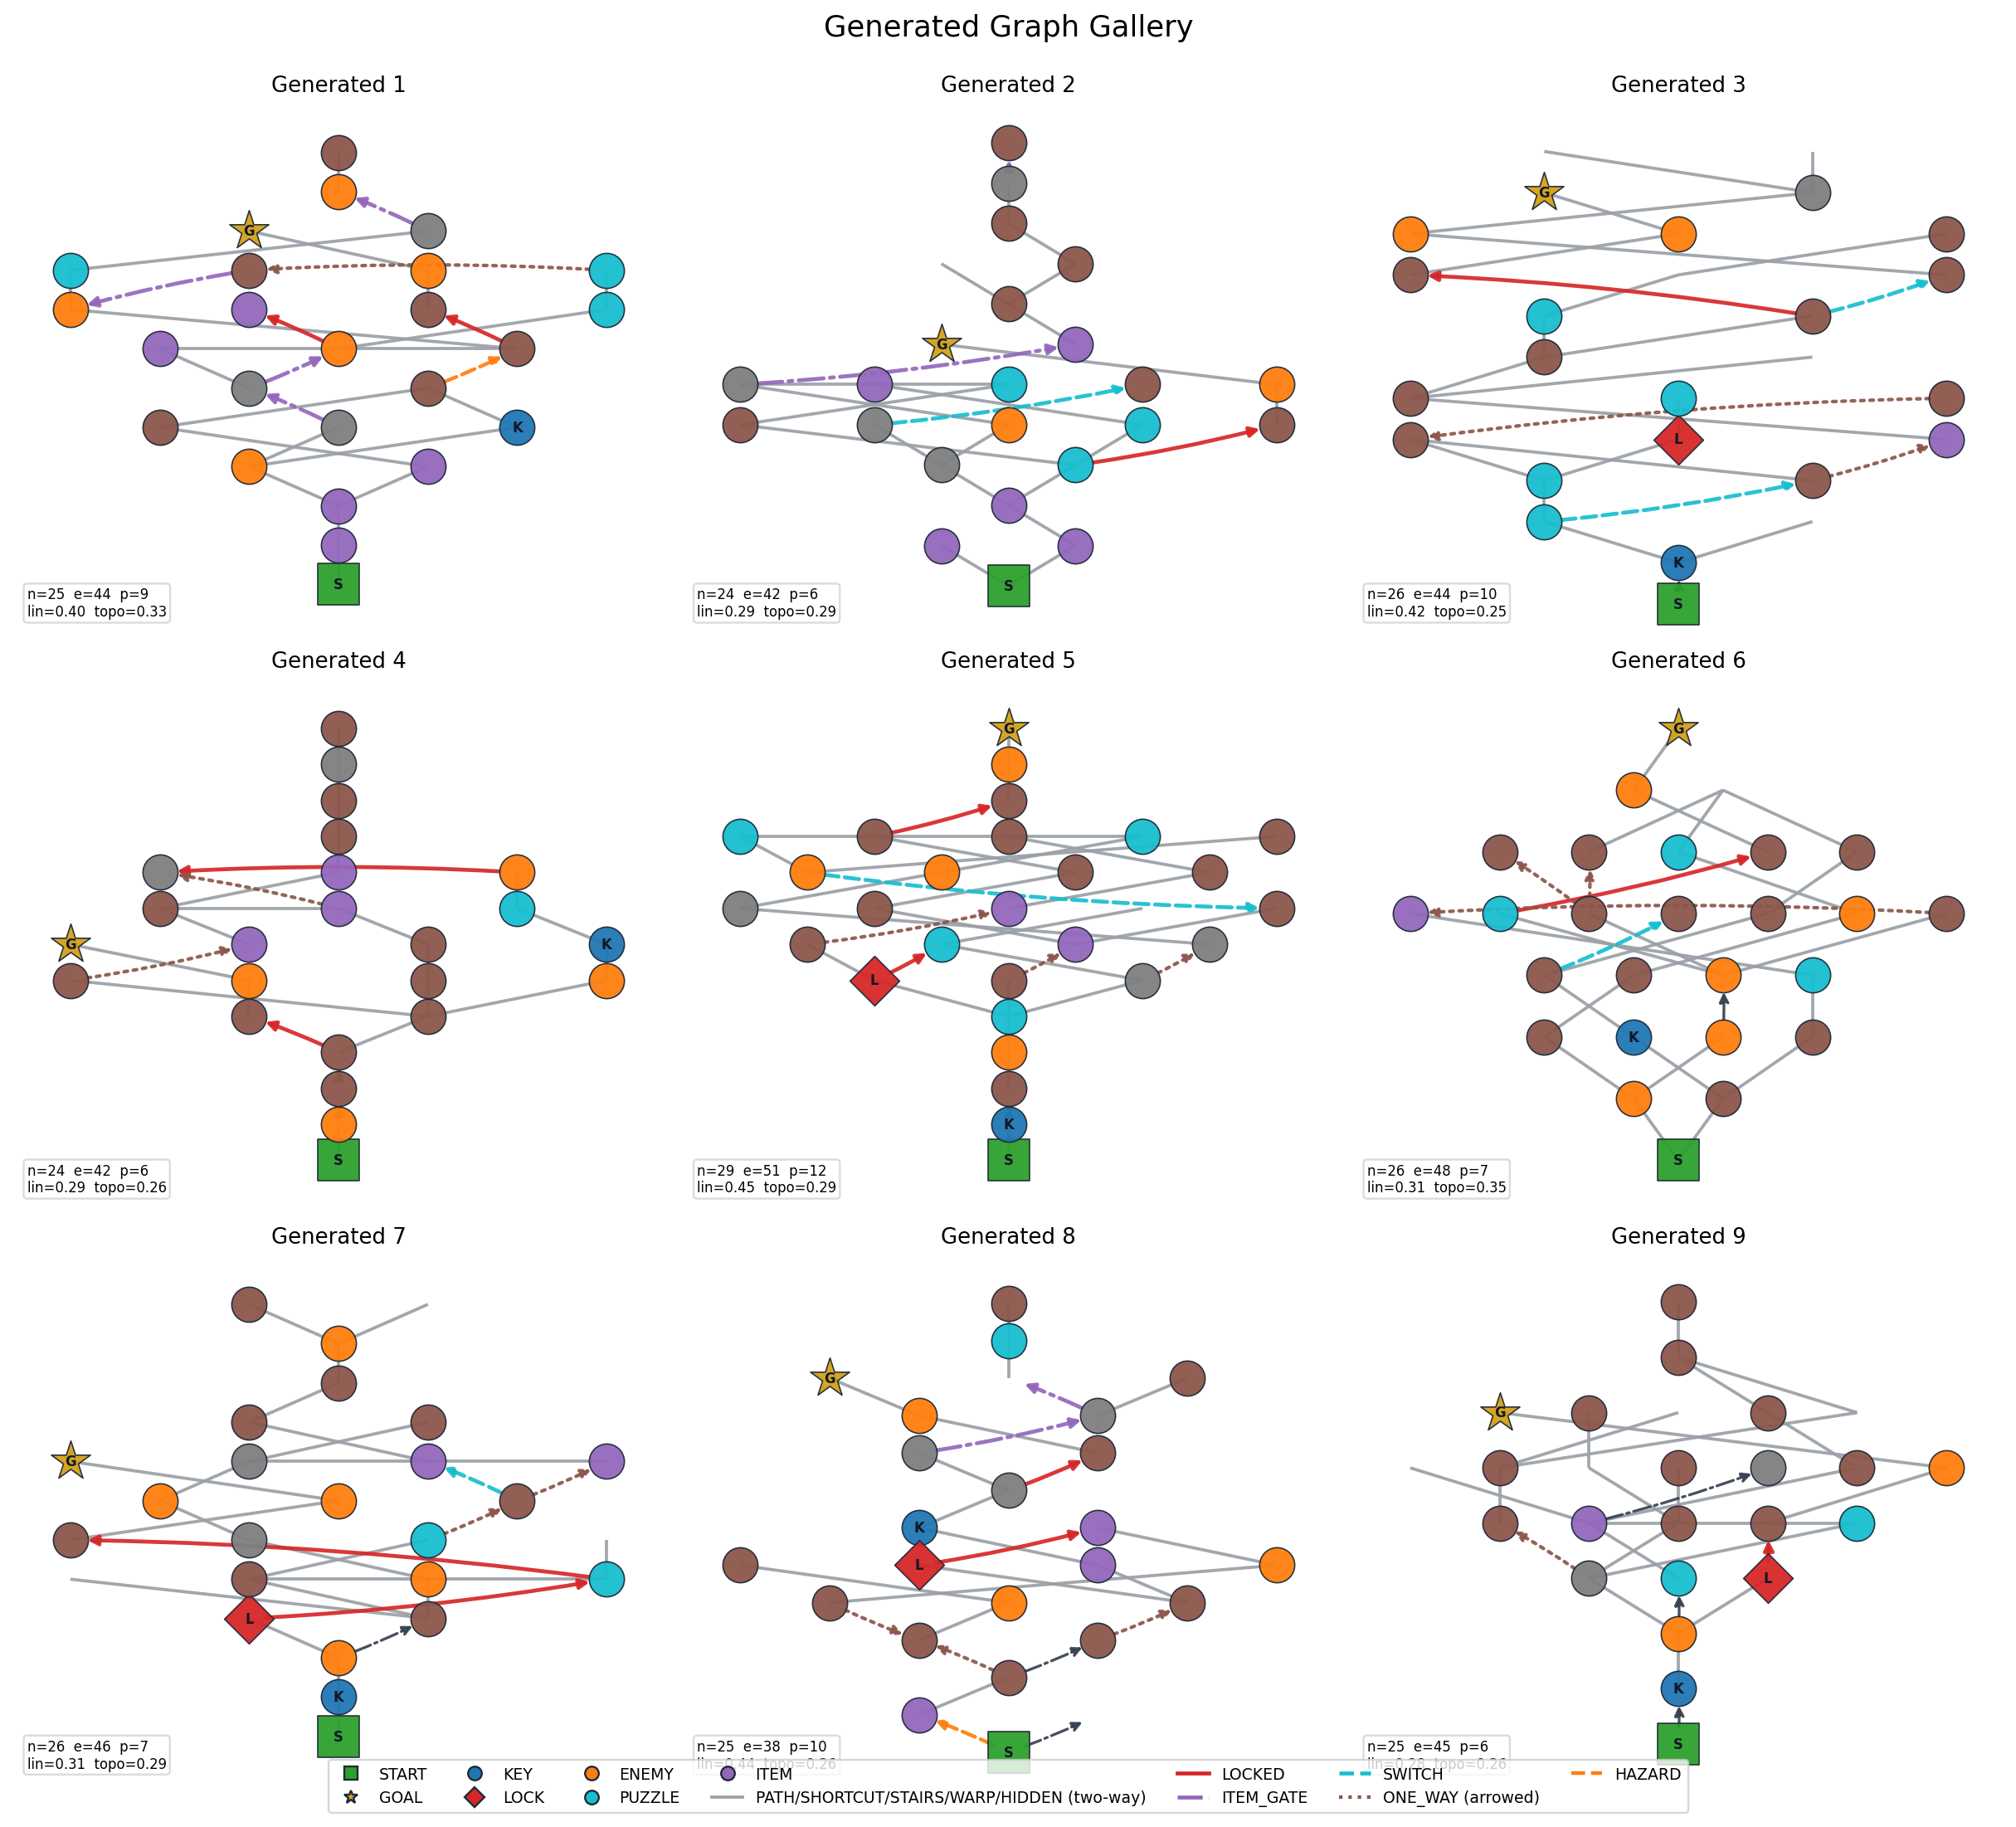
\includegraphics[width=\linewidth]{figures/ch4/real_block_i/generated_gallery.png}
\caption{Gallery đồ thị nhiệm vụ được sinh (seed 42, 8 đồ thị sinh).}
\label{fig:block_i_gallery}
\end{subfigure}

\vspace{0.6em}

\begin{subfigure}[t]{0.66\linewidth}
\centering
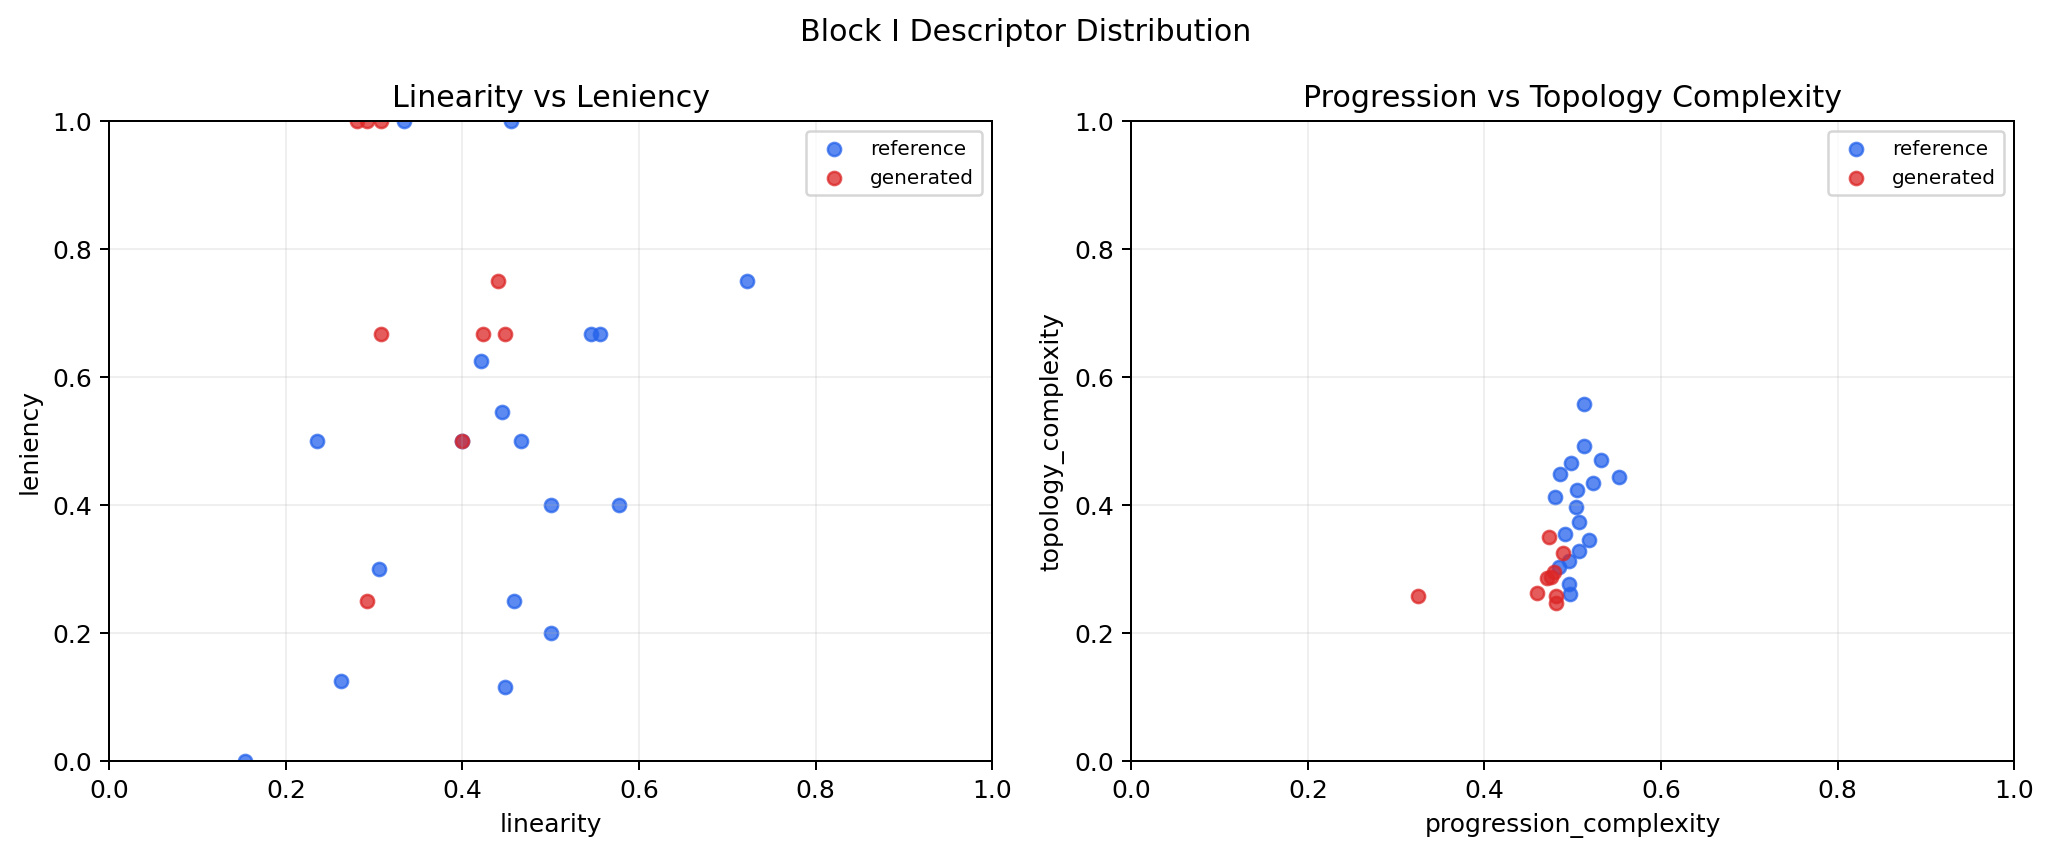
\includegraphics[width=\linewidth]{figures/ch4/real_block_i/descriptor_scatter.png}
\caption{Phân bố descriptor của tập sinh so với tập tham chiếu.}
\label{fig:block_i_descriptor}
\end{subfigure}
\caption{Kết quả sinh đồ thị Block I từ pipeline. Hình được xuất trực tiếp từ pipeline đánh giá, không dùng graph vẽ tay.}
\label{fig:block_i_mission_graph_layout}
\end{figure}

\begin{figure}[H]
\centering
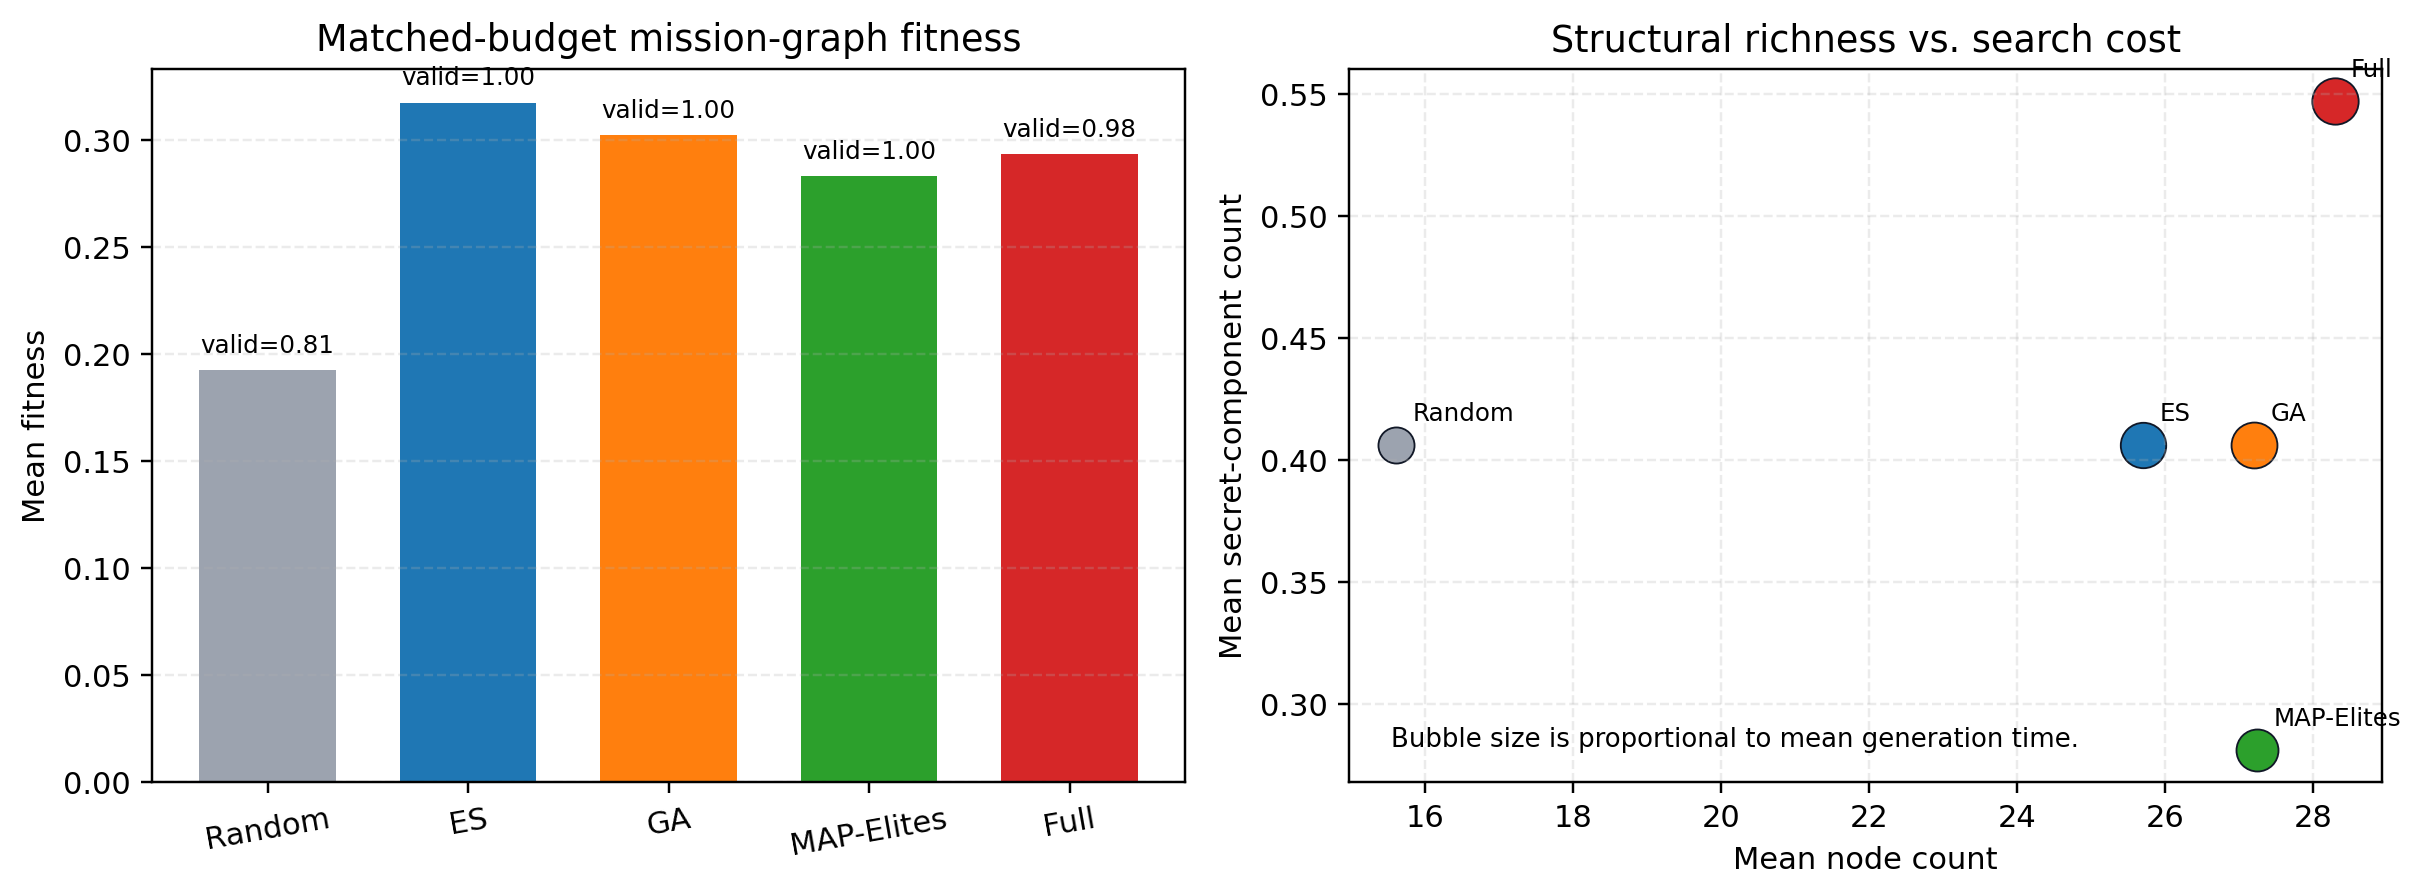
\includegraphics[width=0.96\linewidth]{figures/ch4/mission_graph_matched_budget.png}
\caption{Tổng quan kết quả matched-budget ở Khối I. Biểu đồ trái cho thấy fitness trung bình của từng phương pháp, kèm chú thích về hợp lệ vận hành; biểu đồ phải đối chiếu độ phong phú cấu trúc với chi phí tìm kiếm, trong đó kích thước bong bóng tỉ lệ với thời gian sinh trung bình.}
\label{fig:mission_graph_matched_budget}
\end{figure}

Hình~\ref{fig:mission_graph_matched_budget} làm rõ hơn khác biệt giữa các phương pháp ở Khối I. Nhánh tiến hóa chiến lược đứng đầu về fitness dưới cùng ngân sách, nhưng cấu hình đầy đủ lại dịch sang vùng có số nút trung bình và số thành phần bí mật cao hơn, tức giàu khả năng cấp ngữ nghĩa tiến trình cho tầng sinh phòng hơn. Vì vậy, nếu đọc Khối I như một bài toán sinh đầu vào cho toàn hệ thống chứ không phải chỉ là tối ưu một điểm fitness đơn lẻ, cấu hình đầy đủ vẫn giữ được lý do tồn tại học thuật rõ ràng.

\subsection{Kết quả OOD theo quy mô dungeon}
Thí nghiệm OOD ở tầng đồ thị nhiệm vụ được chia thành ba miền: miền gần phân bố tham chiếu ($18$--$33$ phòng), miền nhỏ hơn ($10$--$16$ phòng) và miền lớn hơn ($35$--$42$ phòng). Bảng~\ref{tab:ood_scaling_results} cho thấy hai phương pháp dùng đầy đủ không gian luật đều giữ được độ hoàn chỉnh tổng thể và độ hợp lệ ràng buộc ở mức $1.0$ trên cả ba miền. Trái lại, biến thể chỉ dùng không gian luật lõi có lợi thế về tốc độ và độ mới, nhưng đánh đổi bằng việc suy giảm mạnh tính hợp lệ.

\begin{table}[H]
\centering
\small
\setlength{\tabcolsep}{4pt}
\renewcommand{\arraystretch}{1.08}
\caption{Kết quả OOD ở tầng đồ thị nhiệm vụ}
\label{tab:ood_scaling_results}
\resizebox{\textwidth}{!}{%
\begin{tabular}{@{}llcccc@{}}
\toprule
Miền kiểm tra & Phương pháp & Hoàn chỉnh tổng thể $\uparrow$ & Hợp lệ ràng buộc $\uparrow$ & Độ mới $\uparrow$ & Thời gian (s) $\downarrow$ \\
\midrule
Gần phân bố & Đầy đủ + GA & \textbf{1.000} & \textbf{1.000} & 0.054 & 14.21 \\
Gần phân bố & Đầy đủ + CVT & \textbf{1.000} & \textbf{1.000} & 0.060 & 11.76 \\
Gần phân bố & Luật lõi + GA & 0.750 & 0.000 & \textbf{0.141} & \textbf{11.11} \\
\midrule
OOD nhỏ & Đầy đủ + GA & \textbf{1.000} & \textbf{1.000} & \textbf{0.064} & 15.21 \\
OOD nhỏ & Đầy đủ + CVT & \textbf{1.000} & \textbf{1.000} & 0.053 & 12.36 \\
OOD nhỏ & Luật lõi + GA & 0.750 & 0.000 & \textbf{0.145} & \textbf{11.23} \\
\midrule
OOD lớn & Đầy đủ + GA & \textbf{1.000} & \textbf{1.000} & 0.042 & 15.71 \\
OOD lớn & Đầy đủ + CVT & \textbf{1.000} & \textbf{1.000} & 0.065 & 12.02 \\
OOD lớn & Luật lõi + GA & 0.750 & 0.000 & \textbf{0.146} & \textbf{11.19} \\
\bottomrule
\end{tabular}%
}
\end{table}

Từ kết quả này có thể rút ra hai nhận xét. Thứ nhất, phần lõi sinh đồ thị nhiệm vụ đang có độ bền tốt trước thay đổi quy mô nếu vẫn giữ đủ không gian luật. Thứ hai, độ mới cao tự nó chưa đủ để thay thế cho tính hợp lệ: phương pháp dùng luật lõi tạo ra đồ thị khác biệt hơn, nhưng sự khác biệt đó đi kèm với mất mát ràng buộc tiến trình.

\clearpage
\begin{figure}[H]
\centering
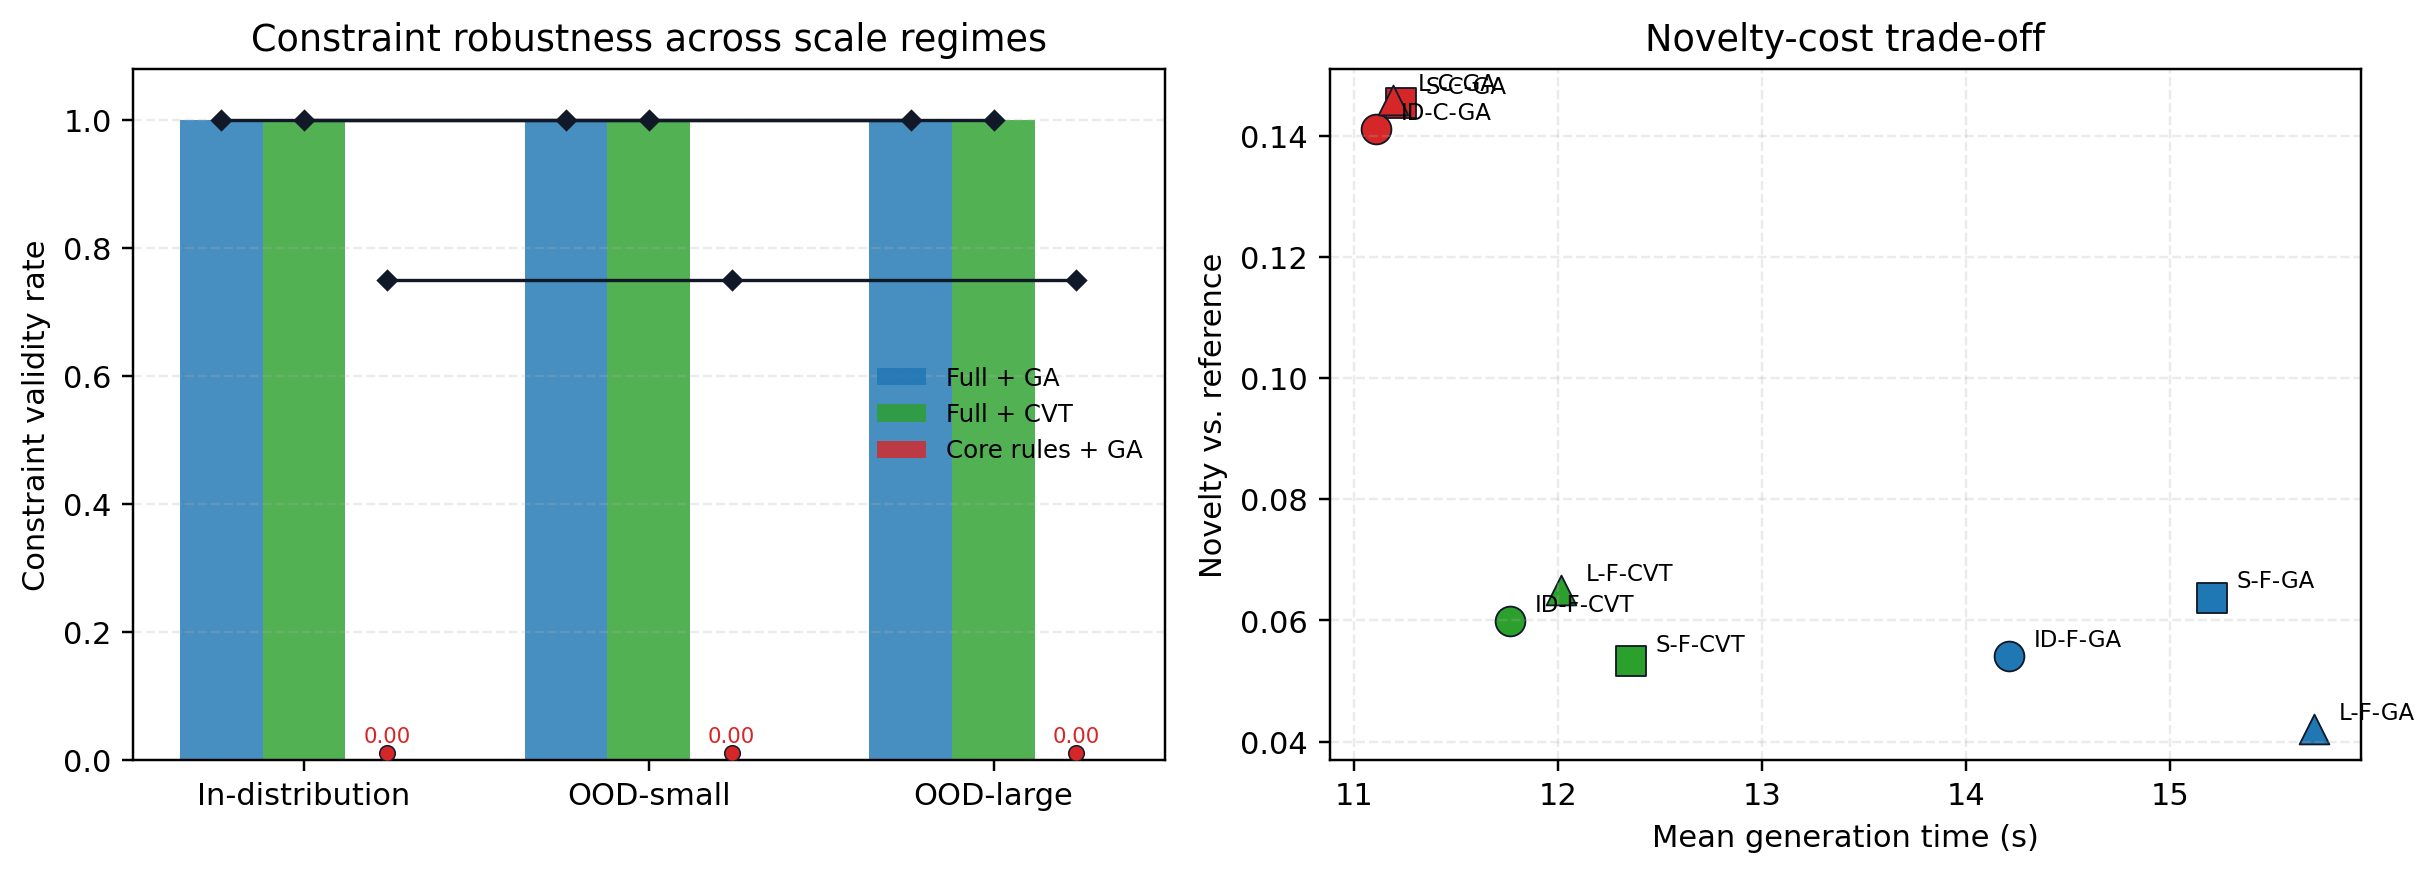
\includegraphics[width=0.94\linewidth]{figures/ch4/topology_robustness_tradeoff.png}
\caption{Độ bền của tầng sinh đồ thị nhiệm vụ theo quy mô và đánh đổi giữa độ mới với chi phí. Ở biểu đồ trái, cột thể hiện tỉ lệ hợp lệ ràng buộc, còn đường kim cương đen biểu diễn độ hoàn chỉnh tổng thể.}
\label{fig:topology_robustness_tradeoff}
\end{figure}

Hình~\ref{fig:topology_robustness_tradeoff} giúp tách rõ hai kiểu kết luận vốn dễ bị trộn lẫn nếu chỉ đọc bảng. Ở biểu đồ trái, hai cấu hình đầy đủ giữ đường hoàn chỉnh tổng thể và cột hợp lệ ràng buộc gần như phẳng ở mức $1.0$ qua cả ba miền, nên có thể xem là bền theo quy mô. Ở biểu đồ phải, biến thể luật lõi dịch về vùng chi phí thấp hơn và độ mới cao hơn, nhưng chính sự dịch chuyển ấy lại đi kèm với việc đánh mất tính hợp lệ; vì vậy, nó phù hợp hơn như một đối chứng cho đánh đổi chứ chưa đủ mạnh để thay thế cấu hình đầy đủ trong đường chạy chính.

\subsection{Độ tin cậy vận hành và chi phí}
Hai nhóm kết quả cuối cùng giúp đọc rõ hơn bài toán vận hành thực tế. Thứ nhất là bộ kiểm thử nhánh sinh phòng ở mức cục bộ với và không với phòng tham chiếu; thứ hai là so sánh ba cấu hình kiểm soát câu đố ở mức dungeon. Bảng~\ref{tab:room_branch_reliability} cho thấy nhánh tiềm ẩn nhanh hơn rõ rệt, trong khi nhánh che khuất đạt tỉ lệ giải được cục bộ cao hơn nhưng phải trả giá bằng chi phí lớn hơn nhiều. Bảng~\ref{tab:puzzle_profile_results} cho thấy cấu hình kiểm soát câu đố mặc định vẫn cho điểm tổng hợp cao nhất, dù cấu hình an toàn tuyến đường có thời gian ngắn hơn đôi chút.

\begin{table}[H]
\centering
\small
\setlength{\tabcolsep}{4pt}
\renewcommand{\arraystretch}{1.08}
\caption{Độ tin cậy và chi phí của các nhánh sinh phòng ở kiểm thử cục bộ}
\label{tab:room_branch_reliability}
\resizebox{\textwidth}{!}{%
\begin{tabular}{@{}lcccc@{}}
\toprule
Cấu hình & Tỉ lệ giải được $\uparrow$ & Chỉ số rối trí $\downarrow$ & Tile sửa TB $\downarrow$ & Thời gian (s) $\downarrow$ \\
\midrule
Tiềm ẩn + có phòng tham chiếu & 0.25 & 6.91 & \textbf{168.00} & 24.74 \\
Tiềm ẩn + không phòng tham chiếu & 0.25 & 6.91 & 168.75 & \textbf{21.34} \\
Che khuất + có phòng tham chiếu & \textbf{0.50} & 8.07 & 172.25 & 64.22 \\
Che khuất + không phòng tham chiếu & \textbf{0.50} & \textbf{5.46} & 174.00 & 60.48 \\
\bottomrule
\end{tabular}%
}
\end{table}

\begin{table}[H]
\centering
\small
\setlength{\tabcolsep}{4pt}
\renewcommand{\arraystretch}{1.08}
\caption{So sánh ba cấu hình kiểm soát puzzle ở mức dungeon}
\label{tab:puzzle_profile_results}
\begin{tabular}{@{}lccc@{}}
\toprule
Cấu hình & Điểm tổng hợp $\uparrow$ & Hard oracle / P-CBS & Thời gian (s) $\downarrow$ \\
\midrule
Mặc định & \textbf{142.603} & Đạt / Đạt & 47.69 \\
An toàn tuyến đường & 123.626 & Đạt / Đạt & \textbf{47.22} \\
Không kiểm soát puzzle & 122.543 & Đạt / Đạt & 48.89 \\
\bottomrule
\end{tabular}
\end{table}

\begin{figure}[H]
\centering
\begin{minipage}[t]{0.32\linewidth}
\centering
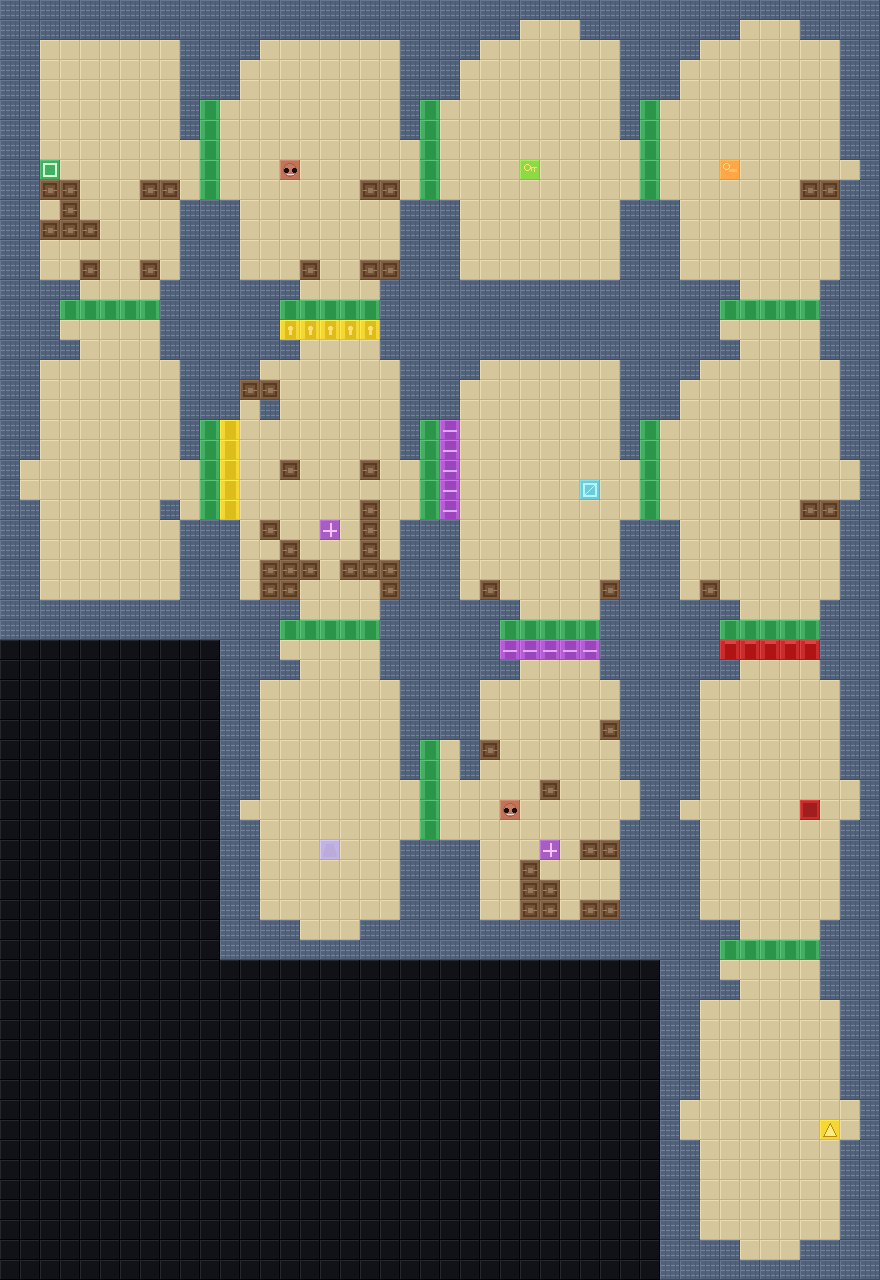
\includegraphics[width=\linewidth]{../results/stateful_puzzle_hparam_sweep_pdrop035_v1/baseline_default/dungeon_grid_stylized.png}
\vspace{1mm}

{\scriptsize (a) Cấu hình mặc định}
\end{minipage}
\hfill
\begin{minipage}[t]{0.32\linewidth}
\centering
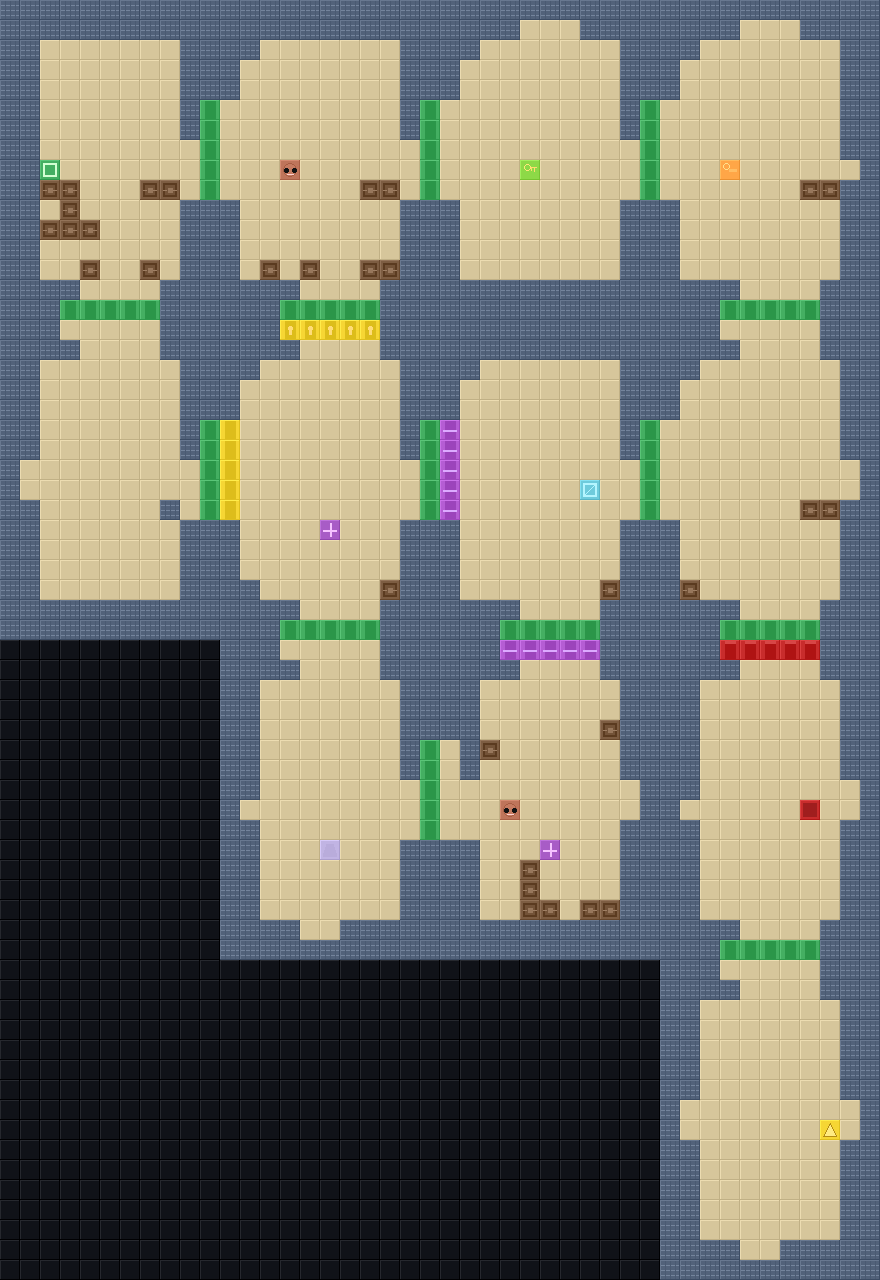
\includegraphics[width=\linewidth]{../results/stateful_puzzle_hparam_sweep_pdrop035_v1/route_safe_stateful/dungeon_grid_stylized.png}
\vspace{1mm}

{\scriptsize (b) Cấu hình an toàn tuyến đường}
\end{minipage}
\hfill
\begin{minipage}[t]{0.32\linewidth}
\centering
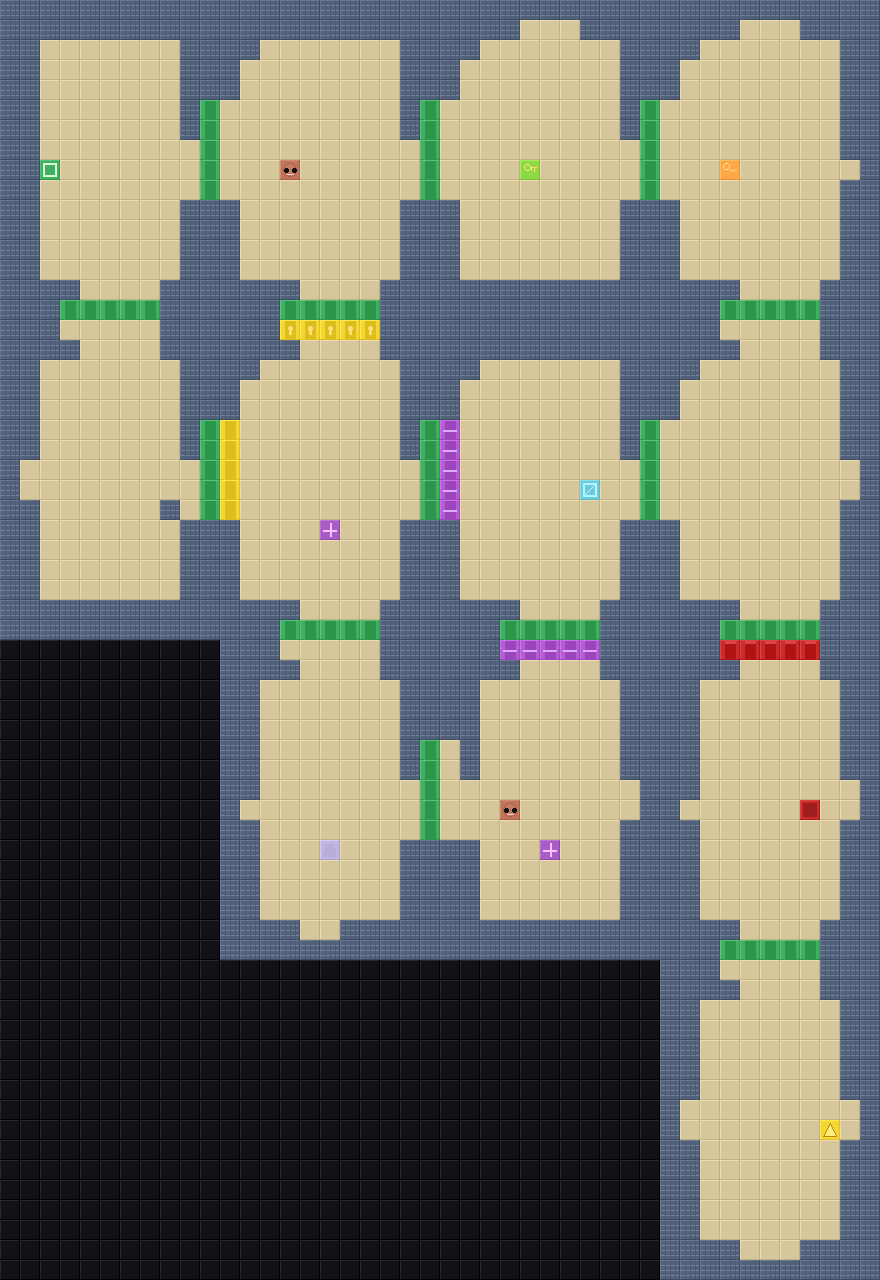
\includegraphics[width=\linewidth]{../results/stateful_puzzle_hparam_sweep_pdrop035_v1/no_puzzle_control/dungeon_grid_stylized.png}
\vspace{1mm}

{\scriptsize (c) Không kiểm soát puzzle}
\end{minipage}
\caption{Ví dụ dungeon sinh ra dưới ba cấu hình kiểm soát puzzle. Cấu hình mặc định giữ được nhiều chi tiết tương tác hơn mà không làm tăng thời gian đáng kể.}
\label{fig:puzzle_profile_examples}
\end{figure}

Khi ghép các kết quả này với Bảng~\ref{tab:overall_generated_graph_compare} và Bảng~\ref{tab:overall_branch_compare}, có thể thấy độ tin cậy vận hành không nên được suy từ một chỉ số duy nhất. Nhánh che khuất có thể cho kết quả hình học khá gần dữ liệu tham chiếu, thậm chí có lợi ở một số kiểm thử cục bộ; tuy nhiên, khi xét đồng thời thời gian đầu-cuối, hợp đồng cơ học và tầng thẩm định nhận thức, nhánh khuếch tán chuẩn vẫn cho điểm cân bằng tốt hơn.

\section{Thảo luận}
\subsection{Giải thích nguồn gốc cải thiện}
Các cải thiện quan sát được phù hợp với logic thiết kế ở Chương 3. Ở tầng phòng, lớp phủ ngữ nghĩa không chỉ ``làm đẹp'' kết quả đầu ra mà thực sự phục hồi lại quan hệ giữa ký hiệu đồ thị và bố trí phòng: trên cấu hình khuếch tán chuẩn, tỉ lệ marker bị ghi đè trước lớp phủ là $29.2\%$, nhưng sau lớp phủ giảm về $0\%$; sai số neo ngữ nghĩa cũng giảm từ $7.875$ về $0$. Vì vậy, đây là một bước khôi phục ngữ nghĩa bắt buộc, không phải một lớp hậu xử lý tùy chọn.

Ở tầng điều khiển, tín hiệu cấu trúc cho hiệu quả rõ hơn tín hiệu ngữ nghĩa theo giai đoạn. Điều khiển cấu trúc vừa giảm thời gian, vừa giảm mức can thiệp hậu kỳ, vừa cải thiện độ gần dữ liệu tham chiếu. Trái lại, tăng cường ngữ nghĩa theo giai đoạn tuy nâng được tỉ lệ qua bộ kiểm tra cơ học, nhưng lại làm mất chấp nhận ở P-CBS. Kết quả này củng cố luận điểm rằng tầng cơ học và tầng nhận thức cần được đọc đồng thời; nếu chỉ nhìn vào một phía, rất dễ kết luận sai về đóng góp của từng khối.

\subsection{Đánh đổi chất lượng, đa dạng và chi phí}
Ba nhóm đánh đổi nổi bật xuất hiện lặp đi lặp lại trong kết quả. Thứ nhất, số bước lấy mẫu ít hơn không đồng nghĩa với toàn hệ nhanh hơn. Nhánh lấy mẫu rút gọn là ví dụ rõ nhất: dù rút gọn pha sinh, thời gian toàn chuỗi vẫn lớn hơn nhiều vì chi phí sửa lỗi và vá marker tăng mạnh. Thứ hai, độ gần dữ liệu tham chiếu chưa chắc đi cùng độ dễ hiểu về mặt nhận thức. Trên đồ thị sinh thật, nhánh nhanh và nhánh che khuất đều có thể giữ hybrid contract và P-CBS, nhưng vẫn kém khuếch tán chuẩn về chi phí; còn trên đồ thị cố định, nhánh che khuất thậm chí còn rơi ở tầng nhận thức. Thứ ba, tăng kích thước codebook hay tăng cường ngữ nghĩa không phải lúc nào cũng mang lợi ích đồng đều trên mọi nhánh; một thay đổi có lợi cho nhánh khuếch tán có thể gây bất lợi cho nhánh che khuất.

Từ đó, cấu hình khuyến nghị trong phạm vi khóa luận là nhánh khuếch tán chuẩn với mức bỏ điều kiện $0.35$, đi kèm cấu hình kiểm soát câu đố mặc định. Trên lượt chạy end-to-end với đồ thị Block~I sinh thật, cấu hình này hoàn thành toàn bộ chuỗi trong \textbf{$21.46$} giây và vượt đồng thời hybrid contract lẫn P-CBS; trên thiết kế đối chứng đồ thị cố định, cùng họ cấu hình tiếp tục cho điểm cân bằng tốt nhất giữa chi phí, mức can thiệp hậu kỳ và độ gần tham chiếu. Nói cách khác, đây không phải cấu hình thắng tuyệt đối ở mọi cột số liệu, nhưng là cấu hình ổn định nhất khi các lớp đánh giá được đọc cùng nhau.

\subsection{Giới hạn}
Giới hạn lớn nhất của Chương 4 là phần lớn so sánh ở tầng sinh phòng vẫn được thực hiện trên một đồ thị nhiệm vụ cố định nhằm giảm nhiễu, trong khi phần end-to-end trên đồ thị sinh thật mới được báo cáo ở một seed đại diện. Cách làm này rất phù hợp để đọc đóng góp biên của từng thành phần, nhưng chưa đủ để tuyên bố ưu thế tổng quát trên toàn bộ không gian cấu trúc. Ngoài ra, thí nghiệm OOD hiện mới kiểm tra trực tiếp tầng đồ thị nhiệm vụ; để khép kín lập luận ở mức hệ thống, cần nối lớp kiểm tra này với toàn bộ chuỗi sinh phòng và hậu kiểm ở các vòng thực nghiệm sau.

Một giới hạn thực dụng khác là chi phí của tầng thẩm định nhận thức còn cao. Các kiểm thử thành phần cho thấy P-CBS đủ giàu để phát hiện khác biệt giữa các cơ chế hành vi, nhưng cũng khiến việc quét rộng nhiều persona và nhiều seed trở nên đắt đỏ. Vì vậy, các kết luận ở mục này nên được hiểu như bằng chứng mạnh về tính khả thi và về các đánh đổi nội tại của kiến trúc, thay vì như một tuyên bố cuối cùng về ưu thế trên mọi điều kiện thử nghiệm.

\section{Tóm tắt chương}
Chương 4 cho thấy kiến trúc đề xuất hoạt động tốt nhất khi được đọc như một hệ nhiều tầng, không phải như một bộ sinh đơn lẻ. Ở mức dungeon hoàn chỉnh, nhánh khuếch tán chuẩn với mức bỏ điều kiện trung bình là cấu hình ổn định nhất cả trên lượt chạy end-to-end với đồ thị sinh thật lẫn trên thiết kế đối chứng đồ thị cố định. Ở mức thành phần, codebook, tín hiệu cấu trúc, tín hiệu ngữ nghĩa và cơ chế kiểm soát câu đố đều để lại ảnh hưởng định lượng rõ ràng lên kết quả cuối. Ở tầng đồ thị nhiệm vụ, thí nghiệm đồng ngân sách và thí nghiệm OOD xác nhận rằng không gian luật đầy đủ giúp hệ giữ tính hợp lệ ổn định hơn khi thay đổi quy mô. Các kết quả này tạo nền trực tiếp cho phần kết luận và định hướng phát triển ở Chương 5.

\chapter{Kết luận và hướng phát triển}
Chương này tổng kết lại các kết quả đã được kiểm chứng và tách rõ giữa điều đã có bằng chứng định lượng với điều vẫn còn là hướng mở. Mỗi kết luận dưới đây đều bám trực tiếp vào các bảng của Chương 4 để tránh phát biểu rộng hơn mức số liệu hiện có.

\section{Tổng kết đóng góp}
Đóng góp thứ nhất của khóa luận là xây dựng được một quy trình sinh dungeon lai nơ-ron -- ký hiệu lấy đồ thị nhiệm vụ làm trục trung tâm, trong đó đồ thị nhiệm vụ giữ vai trò mốc tham chiếu cho tiến trình còn mô hình sinh phòng chịu trách nhiệm hiện thực hóa hình học cục bộ. Giá trị chính của kiến trúc không nằm ở một mô-đun đơn lẻ, mà ở cách các tầng điều kiện hóa, khuếch tán tiềm ẩn, sửa lỗi ký hiệu, bộ kiểm tra cơ học và P-CBS được nối với nhau bằng cùng một quy ước dữ liệu xuyên suốt.

Đóng góp thứ hai là thiết lập được bằng chứng định lượng khá rõ ở tầng sinh phòng, cả trong lượt chạy end-to-end trên đồ thị sinh thật lẫn trong thiết kế đối chứng đồ thị cố định. Cụ thể, Bảng~\ref{tab:overall_generated_graph_compare} cho thấy trên đồ thị nhiệm vụ do Block~I sinh thật, cả ba nhánh đều vượt trọn chuỗi hậu kiểm nhưng nhánh khuếch tán chuẩn giữ chi phí thấp nhất với thời gian đầu-cuối \textbf{$21.46$} giây. Ở phía đối chứng có kiểm soát, Bảng~\ref{tab:overall_branch_compare} tiếp tục cho thấy họ khuếch tán là cấu hình cân bằng nhất giữa thời gian, hậu xử lý và chấp nhận ở tầng nhận thức. Vì vậy, kết luận hợp lệ ở đây không phải là ``khuếch tán thắng mọi cột'', mà là \emph{nhánh khuếch tán chuẩn cho điểm cân bằng tốt nhất giữa chi phí, tính đúng cơ học và mức chấp nhận ở tầng nhận thức trong các thiết lập đã chạy}.

Đóng góp thứ ba là làm rõ được một số đánh đổi cụ thể thay vì chỉ nêu nhận xét chung. Trong Bảng~\ref{tab:pdrop_sweep_results}, mức bỏ điều kiện $0.35$ cho thời gian ngắn nhất (\textbf{$46.49$} giây) và NCD tốt nhất (\textbf{$0.603$}), nhưng mức $0.15$ mới là cấu hình cần ít sửa hậu kỳ nhất (\textbf{$0.917$} so với $1.000$). Trong Bảng~\ref{tab:tokenizer_compare_results}, codebook $512$ cải thiện cho nhánh khuếch tán khi giảm thời gian từ $38.74$ xuống \textbf{$37.82$} giây và giảm NCD từ $0.631$ xuống \textbf{$0.608$}, nhưng cùng thay đổi đó không mang lại lợi ích đồng đều cho nhánh che khuất. Các bảng này cho phép kết luận chặt hơn rằng lợi ích của từng quyết định thiết kế là \emph{phụ thuộc nhánh và phụ thuộc chỉ số}, không thể suy rộng thành ưu thế tổng quát.

Đóng góp thứ tư nằm ở tầng đồ thị nhiệm vụ và tầng nhận thức. Bảng~\ref{tab:matched_budget_results} cho thấy dưới cùng ngân sách $512$ lượt đánh giá, chiến lược tiến hóa thuần đạt điểm thích nghi trung bình cao nhất (\textbf{$0.317$}), còn cấu hình đầy đủ mạnh hơn về độ phong phú cấu trúc với số nút trung bình \textbf{$28.30$} và số thành phần bí mật trung bình \textbf{$0.547$}. Bảng~\ref{tab:ood_scaling_results} cho thấy các cấu hình dùng đầy đủ không gian luật giữ mức hoàn chỉnh tổng thể và hợp lệ ràng buộc bằng $1.0$ trên cả ba miền gần phân phối, OOD nhỏ và OOD lớn, trong khi biến thể luật lõi tụt hợp lệ ràng buộc xuống $0.0$ ở mọi miền. Ở tầng persona, Bảng~\ref{tab:pcbs_ablation_results} cho thấy việc bỏ cơ chế quay lại có kiểm soát hoặc mô hình bất định làm tỉ lệ thành công P-CBS giảm từ $33.3\%$ xuống $16.7\%$ trên bộ sáu bản đồ thử. Trong phạm vi số liệu này, khóa luận có cơ sở để khẳng định rằng không gian luật đầy đủ và hai cơ chế nhận thức nói trên thực sự góp phần giữ ổn định hành vi ở các thiết lập đã chạy.

\section{Hạn chế của nghiên cứu}
Hạn chế thứ nhất là phần lớn so sánh ở tầng sinh phòng vẫn được thực hiện trên một đồ thị nhiệm vụ cố định nhằm giảm nhiễu, trong khi phần end-to-end trên đồ thị sinh thật mới dừng ở một seed đại diện. Thiết kế này rất phù hợp để đọc đóng góp biên của từng thành phần, nhưng chưa đủ để tuyên bố ưu thế tổng quát trên toàn bộ không gian cấu trúc. Vì vậy, các kết luận ở Bảng~\ref{tab:overall_generated_graph_compare}, Bảng~\ref{tab:overall_branch_compare}, Bảng~\ref{tab:pdrop_sweep_results} và Bảng~\ref{tab:tokenizer_compare_results} cần được hiểu là kết luận \emph{trên thiết lập so sánh hiện có}, không phải khẳng định mạnh cho mọi dạng dungeon.

Hạn chế thứ hai là thí nghiệm OOD hiện mới kiểm tra trực tiếp tầng đồ thị nhiệm vụ, chưa khép kín toàn bộ chuỗi từ sinh phòng đến hậu kiểm. Nói cách khác, Bảng~\ref{tab:ood_scaling_results} chứng minh tốt cho độ bền của lớp sinh đồ thị dưới thay đổi quy mô, nhưng chưa đủ để suy rộng ngay sang độ bền của toàn hệ thống nơ-ron--ký hiệu ở mức dungeon hoàn chỉnh.

Hạn chế thứ ba liên quan đến độ rộng của bằng chứng nhận thức. Bảng~\ref{tab:pcbs_ablation_results} chỉ được rút ra từ sáu bản đồ thuộc ba dungeon đầu và một hồ sơ người chơi cân bằng; vì vậy, bảng này đủ mạnh để cho thấy hai cơ chế quay lại có kiểm soát và mô hình bất định là quan trọng trong bộ kiểm thử nhỏ đó, nhưng chưa đủ để kết luận cuối cùng về mọi persona hay mọi họ câu đố. Thêm vào đó, chi phí của tầng P-CBS còn cao, nên việc quét dày nhiều seed và nhiều persona vẫn là một trở ngại thực dụng.

Hạn chế thứ tư là nhánh khuếch tán chính trong hiện thực hiện tại vẫn nạp toàn bộ corpus khi huấn luyện, thay vì duy trì một tập giữ lại độc lập ngay trong vòng lặp tối ưu. Vì vậy, khóa luận chủ động không dùng loss nội bộ của nhánh này như bằng chứng kết luận cuối cùng; các nhận định được đặt chủ yếu trên hậu kiểm sau sinh, so sánh đồng ngân sách và OOD. Đây là một lựa chọn trình bày trung thực với mã nguồn, nhưng cũng đồng nghĩa với việc lớp bằng chứng về tổng quát hóa nội bộ của riêng nhánh khuếch tán vẫn còn mỏng.

\section{Hướng phát triển}
Hướng phát triển gần nhất là mở rộng kiểm thử đầu-cuối sang nhiều cấu trúc đồ thị nhiệm vụ và nhiều seed hơn, để các kết luận ở tầng sinh phòng không còn phụ thuộc mạnh vào một đồ thị nhiệm vụ cố định hay một lượt sinh thật đại diện. Khi đó, các bảng như Bảng~\ref{tab:overall_generated_graph_compare}, Bảng~\ref{tab:overall_branch_compare} hay Bảng~\ref{tab:pdrop_sweep_results} có thể được nâng từ mức ``so sánh trên một kịch bản đại diện'' lên mức ``so sánh đa kịch bản''.

Hướng thứ hai là khép kín thí nghiệm OOD cho toàn quy trình. Thay vì chỉ đánh giá ở tầng đồ thị nhiệm vụ, các vòng sau nên nối OOD với bước sinh phòng, bộ kiểm tra cơ học và P-CBS để xem khi số phòng, độ sâu hoặc mức phân nhánh thay đổi thì toàn chuỗi còn giữ được đồng thời tính đúng cơ học, mức dễ hiểu nhận thức và chi phí vận hành hay không.

Hướng thứ ba là mở rộng lớp đánh giá nhận thức. Về mặt thuật toán, cần quét dày hơn không gian tham số persona và kiểm tra trên tập bản đồ lớn hơn; về mặt thực nghiệm, nên từng bước nối P-CBS với đánh giá người chơi hoặc ít nhất là các proxy hành vi mạnh hơn để kiểm tra xem các chỉ số như CGR, $H_{\mathrm{nav}}$ và \emph{goal-sighting latency} tương ứng tốt đến đâu với trải nghiệm thật.

Cuối cùng, cần chuẩn hóa lại toàn bộ luồng báo cáo để các bảng loại trừ, đồng ngân sách và OOD được sinh tự động từ cùng một quy trình. Khi đó, khóa luận không chỉ mạnh hơn ở mặt kiến trúc, mà còn mạnh hơn ở khả năng tái lập và cập nhật kết quả khi mô hình, dữ liệu hoặc giao thức đánh giá tiếp tục thay đổi.

\FloatBarrier
\clearpage
\renewcommand{\bibname}{Tài liệu tham khảo}
\clearpage
\phantomsection
\addcontentsline{toc}{chapter}{Tài liệu tham khảo}
\bibliographystyle{ieeetr}
\bibliography{references}

\clearpage
\appendix
\chapter*{PHỤ LỤC}
\addcontentsline{toc}{chapter}{PHỤ LỤC}
\setcounter{section}{0}
\setcounter{subsection}{0}
\renewcommand{\thesection}{\Alph{section}}
\renewcommand{\thesubsection}{\thesection.\arabic{subsection}}

Phụ lục được tổ chức theo hai trục song song để người đọc vừa tra cứu được phần \emph{thuật toán/chứng minh}, vừa có đủ phần \emph{minh họa/đối chiếu} với dữ liệu và đầu ra. Các mục dưới đây giữ lại những gì trực tiếp hỗ trợ việc kiểm tra lại phương pháp và kết quả; những đoạn mã nguồn quá dài hoặc lặp lại gần như nguyên văn với mô tả ở bản chính đã được lược bỏ.

\section{Minh họa và đối chiếu trực quan}
\label{app:visual_audits}

Phần này bổ sung các hình ảnh mà bản chính không thể giữ hết vì giới hạn dung lượng. Mục tiêu là cho người đọc thấy rõ hơn mối liên hệ giữa vai trò phòng, hình học lưới và cấu hình puzzle ở các kết quả đã được dùng để lập bảng trong Chương 4.

\begin{figure}[H]
\centering
\begin{minipage}[t]{0.46\linewidth}
\centering
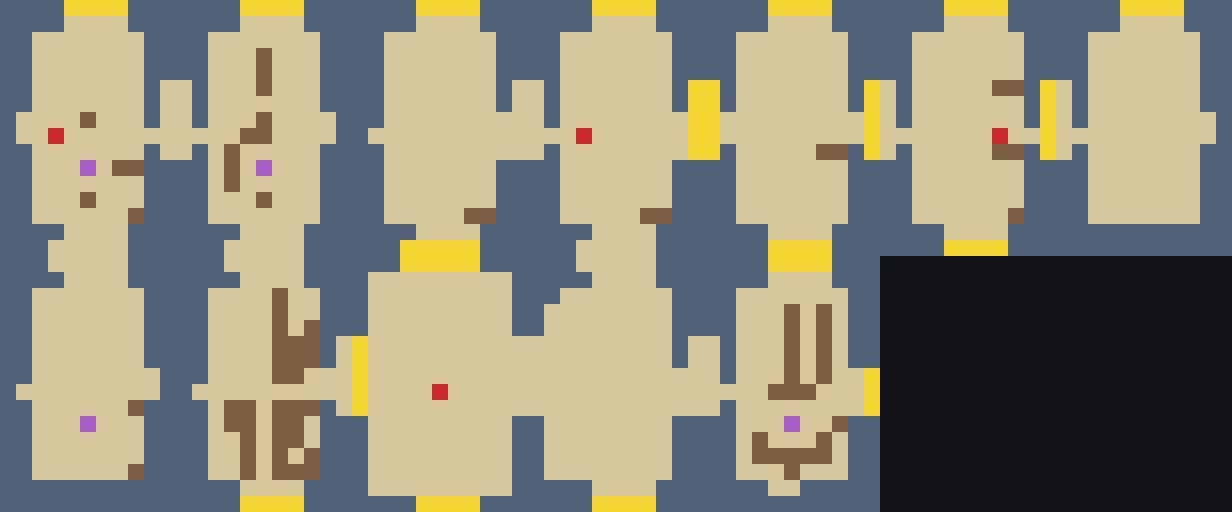
\includegraphics[width=\linewidth]{../results/ch4_generated_topology_real_pdrop035_seed20260418_fixedvalidator/diffusion_cfg3_logic0_steps50/dungeon_grid_readable.png}
\vspace{1mm}

{\scriptsize (a) Bản đồ đọc được của cấu hình khuếch tán trên đồ thị sinh thật}
\end{minipage}
\hfill
\begin{minipage}[t]{0.50\linewidth}
\centering
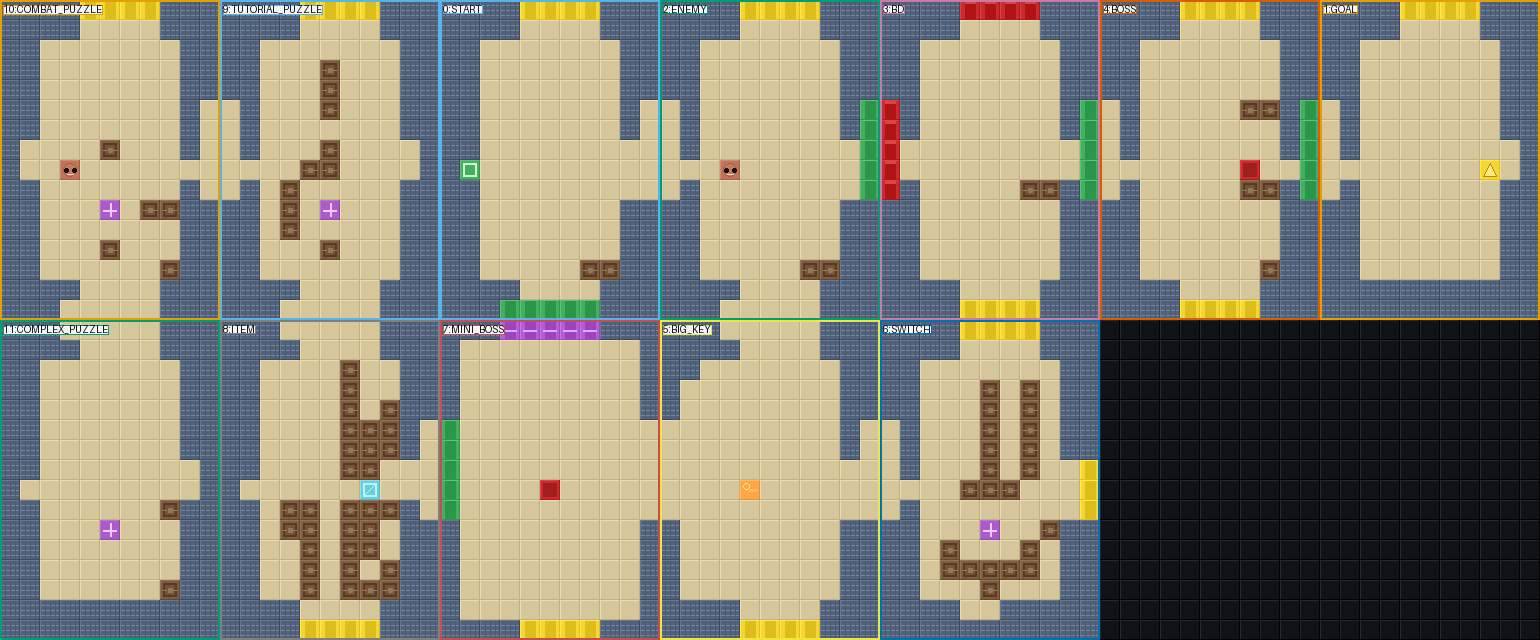
\includegraphics[width=\linewidth]{../results/ch4_generated_topology_real_pdrop035_seed20260418_fixedvalidator/diffusion_cfg3_logic0_steps50/dungeon_grid_alignment.png}
\vspace{1mm}

{\scriptsize (b) Cùng dungeon nhưng gắn nhãn vai trò phòng}
\end{minipage}
\caption{Hai góc nhìn bổ sung cho cùng một dungeon end-to-end trên đồ thị sinh thật. Hình (a) cho thấy bản đồ ở dạng dễ đọc; hình (b) cho thấy cách các vai trò phòng và các cửa có điều kiện được phân bố trên cùng bố cục đó.}
\label{fig:appendix_diffusion_alignment}
\end{figure}

\begin{figure}[H]
\centering
\begin{minipage}[t]{0.49\linewidth}
\centering
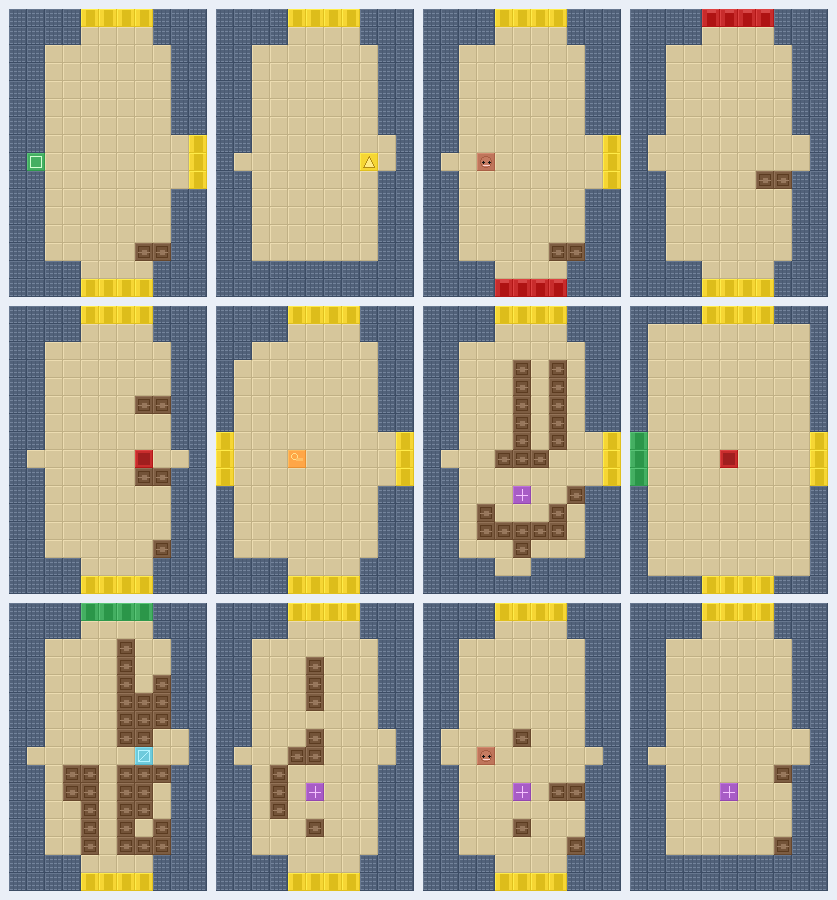
\includegraphics[width=\linewidth]{../results/ch4_generated_topology_real_pdrop035_seed20260418_fixedvalidator/diffusion_cfg3_logic0_steps50/rooms_sheet_stylized.png}
\vspace{1mm}

{\scriptsize (a) Tập phòng của lượt chạy end-to-end thật}
\end{minipage}
\hfill
\begin{minipage}[t]{0.49\linewidth}
\centering
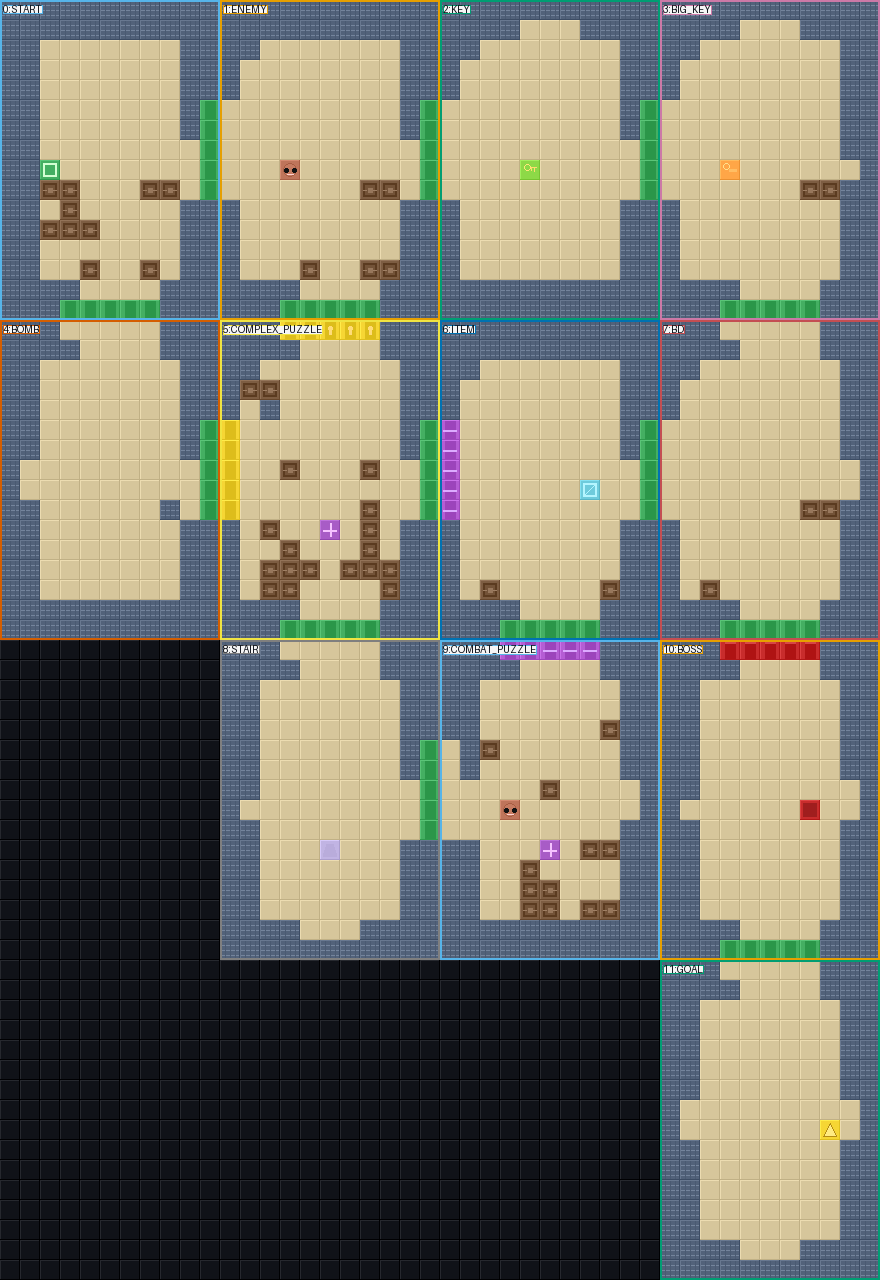
\includegraphics[width=\linewidth]{../results/stateful_puzzle_hparam_sweep_pdrop035_v1/baseline_default/dungeon_grid_alignment.png}
\vspace{1mm}

{\scriptsize (b) Cấu hình puzzle mặc định với chồng lớp vai trò}
\end{minipage}
\caption{Đối chiếu trực quan ở cấp phòng và cấp dungeon. Hình (a) cho thấy toàn bộ các phòng được hệ sinh ra trên cùng một lần chạy end-to-end thật; hình (b) minh họa cách cấu hình kiểm soát puzzle mặc định tổ chức các vai trò như key, item, boss và goal trên bản đồ hoàn chỉnh.}
\label{fig:appendix_room_sheet_and_puzzle_alignment}
\end{figure}

\section{Khung ký hiệu và mô hình chi phí}
\label{app:cost_model}

\subsection{Ký hiệu sử dụng trong phụ lục}
Ngoài các ký hiệu đã nêu ở Chương 3, phụ lục dùng thêm các đại lượng dưới đây để tường minh hóa phép đếm chi phí:
\begin{equation}
C_{\text{enc}},\; C_{\text{diff}},\; C_{\text{logic}},\; C_{\text{logicnet}},\; C_{\text{batch}},\; C_{\text{teacher}},\; C_{\text{handoff}},\; C_{\text{hard}},\; C_{\text{pcbs}},\; C_{\text{archive}}.
\end{equation}
Mỗi đại lượng biểu thị chi phí thời gian của một khối chức năng tương ứng trong một lần gọi ở mức trừu tượng thuật toán. Riêng $C_{\text{pcbs}}$ được hiểu là chi phí cho một persona; nếu đánh giá trên tập persona $\mathcal{P}$ thì phần đóng góp tương ứng có bậc $|\mathcal{P}|\,C_{\text{pcbs}}$.

\subsection{Mô hình chi phí chuẩn hóa}
Phân tích trong phụ lục dùng mô hình chi phí chuẩn hóa theo số phép toán sơ cấp và số lần gọi khối xử lý. Mô hình này phục vụ so sánh thứ bậc tăng trưởng giữa các thuật toán, không thay thế phép đo thời lượng thực thi trên phần cứng cụ thể.

\section{Thuật toán bổ trợ trong phụ lục}
\label{app:supplementary_algorithms}

Phần này ghi lại các thuật toán phụ trợ được rút gọn từ phần phương pháp chính, chủ yếu gồm các bước tiền xử lý, chia tập và kiểm tra hợp lệ-khả giải. Các thuật toán cốt lõi dựa trên tìm kiếm đã được mô tả ở Chương 3; phụ lục chỉ giữ lại các bước hỗ trợ thường đi kèm để tiện tra cứu.

\subsection{Tiền xử lý dữ liệu phòng và tách tập cho các nhánh huấn luyện}
\begin{algorithm}[H]
\caption{Tiền xử lý dữ liệu phòng và tách tập cho các nhánh huấn luyện}
\label{alg:preprocess_data_split}
\begin{algorithmic}[1]
\Require Corpus dungeon thô $\mathcal{D}_{\text{raw}}$, seed $s$, tỉ lệ kiểm định nội bộ $\rho_{\mathrm{val}}$
\Ensure Tập phòng chuẩn hóa $\mathcal{D}_{\text{room}}$, tập huấn luyện $\mathcal{D}_{\text{train}}$, tập kiểm định $\mathcal{D}_{\text{val}}$ và toàn bộ corpus cho nhánh khuếch tán
\State Đọc lần lượt các dungeon nguồn và đồ thị nhiệm vụ tương ứng
\State Đối sánh mỗi phòng vật lý với nút đồ thị tương ứng để khôi phục quan hệ hình học--tiến trình
\State Tách từng phòng về kích thước chuẩn $16\times 11$ và gắn siêu dữ liệu cửa, nội dung, vị trí
  \State Dựng các tensor đặc trưng nút/cạnh, mã hóa theo thứ tự topo, ràng buộc biên và bản đồ phòng lân cận
\State Loại các mẫu có kích thước sai hoặc chứa giá trị không hữu hạn
\State Chuẩn hóa các lưới còn lại về miền mã tile cố định, thu $\mathcal{D}_{\text{room}}$
\State Trộn xác định $\mathcal{D}_{\text{room}}$ bằng seed $s$
\State Tách ngẫu nhiên nhưng tái lập được $\mathcal{D}_{\text{room}}$ theo tỉ lệ $(1-\rho_{\mathrm{val}},\rho_{\mathrm{val}})$ cho các nhánh học ở mức phòng
\State Giữ toàn bộ $\mathcal{D}_{\text{room}}$ làm corpus huấn luyện cho nhánh khuếch tán chính
\State \Return $\mathcal{D}_{\text{room}},\mathcal{D}_{\text{train}},\mathcal{D}_{\text{val}}$
\end{algorithmic}
\end{algorithm}

\subsection{Kiểm tra hợp lệ và khả giải dungeon}
\begin{algorithm}[H]
\caption{Kiểm tra hợp lệ và khả giải dungeon trước khi đưa vào kho lưu trữ}
\label{alg:dungeon_validity_solvability}
\begin{algorithmic}[1]
\Require Dungeon đã ghép $D$, đồ thị vật lý $G_{\mathrm{phys}}$, cặp start-goal $(s,g)$
\Ensure Cờ hợp lệ $v$, cờ khả giải $u$, và bộ chẩn đoán $\mathcal{I}$
\State $v \gets 1$, $u \gets 0$, $\mathcal{I} \gets \varnothing$
\State Kiểm tra kích thước phòng, biên ngoài, và tính nhất quán cửa-biên
\If{không thỏa}
  \State $v \gets 0$
  \State Ghi chẩn đoán lỗi hình học vào $\mathcal{I}$
  \State \Return $v,u,\mathcal{I}$
\EndIf
\State Kiểm tra liên thông trên $G_{\mathrm{phys}}$ và trên lưới ghép
\If{không liên thông}
  \State $v \gets 0$
  \State Ghi chẩn đoán lỗi liên thông vào $\mathcal{I}$
  \State \Return $v,u,\mathcal{I}$
\EndIf
\State Kiểm tra reachability từ $s$ đến $g$
\State Kiểm tra các ràng buộc khóa--cổng, vật phẩm và boss gate nếu có
\If{mọi kiểm tra đều đạt}
  \State $u \gets 1$
\Else
  \State Ghi chẩn đoán lỗi tiến trình vào $\mathcal{I}$
\EndIf
\State \Return $v,u,\mathcal{I}$
\end{algorithmic}
\end{algorithm}

Năm thuật toán dưới đây bổ sung các khối hậu xử lý và điều phối còn lại của quy trình; chúng được giữ ở phụ lục để người đọc có thể tra cứu nhanh mà không phải quay lại toàn bộ phần phương pháp.

\subsection{Sửa phòng có phản hồi ký hiệu}
\begin{algorithm}[H]
\caption{Sửa phòng có phản hồi ký hiệu ở tầng hậu xử lý}
\label{alg:app_room_repair_feedback}
\begin{algorithmic}[1]
\Require Lưới nơ-ron đầu vào $x_i^{\text{neural}}$, đồ thị phòng $G_i$, cặp start-goal $(s_i,g_i)$
\Ensure Lưới cuối $x_i^{\text{final}}$ thỏa ràng buộc biên và đường đi
\State $x_i^{\text{final}} \gets$ Chuẩn hóa mã ngữ nghĩa của $x_i^{\text{neural}}$ về từ điển tile hợp lệ
\State $x_i^{\text{final}} \gets$ Loại bỏ các marker biến động không nên bảo lưu ở đầu ra phòng
\State $x_i^{\text{final}} \gets$ Khôi phục vỏ biên theo ràng buộc cửa-biên của $G_i$
\State $m_i \gets$ Dựng dấu vết kế hoạch từ $G_i$ và cặp $(s_i,g_i)$
\If{bước sửa hậu kỳ được kích hoạt}
  \State $x_i^{\text{cand}} \gets$ Sinh ứng viên sửa có phản hồi ký hiệu từ $x_i^{\text{final}}$ và $m_i$
  \If{bước sửa tạo ra cấu hình hợp lệ}
    \State $x_i^{\text{final}} \gets x_i^{\text{cand}}$
  \EndIf
\EndIf
\State $x_i^{\text{final}} \gets$ Chồng các marker tiến trình từ đồ thị lên lưới đã sửa
\State Kiểm tra lại kích thước phòng và tính hợp lệ hình học của $x_i^{\text{final}}$
\State \Return $x_i^{\text{final}}$
\end{algorithmic}
\end{algorithm}

Thuật toán này đóng vai trò cầu nối giữa chất lượng hình học và tính đúng gameplay ở cấp phòng.

\subsection{Lập lịch sinh phòng theo lớp phụ thuộc}
\begin{algorithm}[H]
\caption{Lập lịch sinh phòng theo lớp phụ thuộc}
\label{alg:app_layer_bucket_scheduler}
\begin{algorithmic}[1]
\Require Đầu vào đã chuẩn bị $(G_{phys}, C)$, cấu hình sinh phòng
\Ensure Tập kết quả phòng $\mathcal{R}$, latent phòng và chẩn đoán theo lô
\If{chế độ sinh theo lô các phòng độc lập được kích hoạt và $G_{phys}$ có hướng}
  \State Phân lớp topo trên $G_{phys}$, thu $\mathcal{L}$
  \ForAll{lớp $\ell \in \mathcal{L}$}
    \State Gom các phòng trong $\ell$ theo nhóm latent, thu $\mathcal{B}$
    \ForAll{nhóm $b \in \mathcal{B}$}
      \If{kích thước phòng không chuẩn $(16,11)$}
        \State Sinh tuần tự từng phòng trong $b$
      \Else
        \State Ước lượng kích thước mảnh an toàn $k$ theo ngân sách bộ nhớ
        \ForAll{mảnh độc lập kích thước $k$ trong $b$}
          \State Sinh lô phòng cho mảnh hiện tại, thu $\mathcal{R}_{chunk}$
          \State Cập nhật $\mathcal{R}$ và latent đã sinh
        \EndFor
      \EndIf
    \EndFor
  \EndFor
\Else
  \State Sinh tuần tự theo thứ tự nút ổn định
\EndIf
\State \Return $\mathcal{R}$, latent phòng, chẩn đoán theo lô
\end{algorithmic}
\end{algorithm}

Thuật toán này điều phối việc sinh nhiều phòng theo lớp topo và nhóm latent, nhờ đó bảo toàn các phụ thuộc logic giữa các phòng.

\subsection{Sinh một phòng với bước quay về mô hình giáo viên}
\begin{algorithm}[H]
\caption{Sinh một phòng với bước quay về mô hình giáo viên}
\label{alg:app_generate_room_fallback}
\begin{algorithmic}[1]
\Require Điều kiện phòng $(z_N,z_S,z_E,z_W,b_i,p_i,G_i)$, cấu hình bộ lấy mẫu
\Ensure Kết quả sinh phòng cho phòng $i$
\State $c_i \gets$ Kết hợp ngữ cảnh lân cận, ràng buộc biên và ngữ cảnh đồ thị
\If{chế độ suy luận là nhánh che khuất rời rạc}
  \State Lấy mẫu latent che khuất và phân bố dự đoán cho phòng, thu $(z_i,\ell_i)$
\ElsIf{chế độ suy luận là nhánh codebook rời rạc}
  \State Lấy mẫu theo tập mã rời rạc có điều kiện, thu $(z_i,\ell_i)$
\Else
  \State $z_i \gets$ Lấy mẫu latent bằng mô hình khuếch tán đầy đủ dưới CFG và dẫn dắt logic
  \State $\ell_i \gets$ Giải mã $z_i$ thành phân bố dự đoán trên lưới phòng
\EndIf
\State $x_i^{\text{neural}} \gets \arg\max\ell_i$
\State $x_i^{\text{final}} \gets$ Hiệu chỉnh ký hiệu và khôi phục vỏ biên từ $x_i^{\text{neural}}$
\If{cần quay về mô hình giáo viên}
  \State Sinh lại bằng mô hình giáo viên đầy đủ và vô hiệu hóa bước quay về lồng nhau
\EndIf
\State \Return $(x_i^{\text{final}}, z_i, \text{metrics})$
\end{algorithmic}
\end{algorithm}

Thuật toán này đóng vai trò lớp an toàn cho nhánh lấy mẫu nhanh ở cấp một phòng.

\enlargethispage{2\baselineskip}
\subsection{Chuẩn hóa trước khi kiểm tra cơ học và P-CBS}
\begin{algorithm}[H]
\caption{Chuẩn hóa dungeon đã ghép trước khi kiểm tra cơ học và P-CBS}
\label{alg:app_validation_handoff_normalization}
\begin{algorithmic}[1]
\Require Dungeon đã ghép $D$, tùy chọn cặp terminal $(s,g)$
\Ensure Dungeon chuẩn hóa $D^\star$, terminal hợp lệ và bộ chẩn đoán chuẩn hóa $\mathcal{I}_{\mathrm{handoff}}$
\State $D^\star \gets$ Ép kiểu dungeon về lưới số nguyên hợp lệ
\State Ánh xạ mọi mã ngữ nghĩa ngoài bảng từ điển về tile hợp lệ mặc định
\State Đánh dấu \texttt{VOID} ngoại biên bằng phép tô loang từ đường biên ngoài
\State Lấp mọi \texttt{VOID} kín không nối ra biên bằng tile tường
\State Chuẩn hóa đúng một \texttt{START} và đúng một \texttt{TRIFORCE}
\If{$s$ và $g$ trùng nhau sau chuẩn hóa}
  \State Báo lỗi chuẩn hóa không hợp lệ và dừng
\EndIf
\State Ghi các thống kê: số tile ngoài bảng từ điển, số \texttt{VOID} kín đã lấp, số terminal trùng bị loại
\State \Return $D^\star,(s,g),\mathcal{I}_{\mathrm{handoff}}$
\end{algorithmic}
\end{algorithm}

Thuật toán này làm tường minh ranh giới giữa tầng sinh dungeon và tầng thẩm định, nhờ đó bộ kiểm tra cơ học và P-CBS luôn làm việc trên cùng một miền dữ liệu chuẩn hóa.

\enlargethispage{2\baselineskip}
\subsection{Đánh giá dungeon sau ghép}
\begin{algorithm}[H]
\caption{Đánh giá dungeon sau ghép với bước chuẩn hóa, kiểm tra cơ học và P-CBS}
\label{alg:app_post_generation_evaluation}
\begin{algorithmic}[1]
\Require Dungeon đã ghép $D$, tập phòng $\mathcal{R}$, đồ thị vật lý $G_{phys}$, tập persona $\mathcal{P}$
\Ensure Chẩn đoán chuẩn hóa, phán quyết cơ học, chỉ số P-CBS/QD và danh sách phòng lỗi
\State Chuẩn hóa dungeon trước thẩm định, thu $D^\star$ và $\mathcal{I}_{\mathrm{handoff}}$
\State Thẩm định cơ học cứng trên $D^\star$, thu $s_{\mathrm{hard}}$
\If{$s_{\mathrm{hard}}$ thỏa điều kiện giải được}
  \ForAll{$p \in \mathcal{P}$}
    \State Chạy P-CBS cho persona $p$, thu $m_p$
  \EndFor
  \If{bật MAP-Elites và thành phần MAP-Elites khả dụng}
    \State Cập nhật kho lưu trữ MAP-Elites bằng dungeon hợp lệ $D^\star$
    \State Trích xuất các chỉ số QD từ $D^\star$
  \EndIf
\EndIf
\If{LogicNet khả dụng}
  \ForAll{phòng $r_i \in \mathcal{R}$ có latent}
    \State Suy diễn LogicNet trên latent phòng, thu $(\ell_i,info_i)$
    \State Cộng dồn $\mathrm{grid\_reach}_i$ và ghi phòng lỗi nếu dưới ngưỡng
  \EndFor
\EndIf
\State \Return $\mathcal{I}_{\mathrm{handoff}}, s_{\mathrm{hard}}, \{m_p\}_{p\in\mathcal{P}}$ cùng các chỉ số QD và danh sách phòng lỗi
\end{algorithmic}
\end{algorithm}

Thuật toán này chốt vòng đánh giá hậu sinh ở cấp dungeon và cấp phòng, đồng thời giữ nhất quán với đường chạy thẩm định đã mô tả trong Chương 3.

\FloatBarrier
\section{Trích đoạn dữ liệu mở rộng và bảng luật chi tiết}
\label{app:data_rules}

\subsection{Trích đoạn dữ liệu mở rộng}
Chương~3 đã giới thiệu quy ước ký hiệu ASCII, một mẫu trích đoạn ngắn và các luật gameplay cốt lõi theo đúng trình tự của phương pháp. Phụ lục này chỉ giữ lại ba trích đoạn dài hơn từ corpus nguồn để người đọc đối chiếu trực tiếp với dữ liệu thô, đồng thời lưu bảng luật chi tiết phục vụ kiểm tra chéo với hiện thực mã nguồn.

\begin{lstlisting}[caption={Trích đoạn dungeon nhỏ từ corpus Zelda nguồn},label={lst:dataset_small_sample},basicstyle=\ttfamily\tiny,breaklines=false,columns=fullflexible,xleftmargin=0.2em,framexleftmargin=0.2em]
WWWWWWWWWWW-----------WWWWWWWWWWWWWWWWWWWWWW-----------WWWWWWWWWWW
WWWWWWWWWWW-----------WWWWDDDWWWWWWWWWWWWWWW-----------WWWWWWWWWWW
WWFFFFFFFWW-----------WWFFFFFFFWWWWFFFFFFFWW-----------WWFFFFFFFWW
WWFFFFFFFWW-----------WWFFFFFFFWWWWFFFFFFFWW-----------WWFFFFFFFWW
WWFFFFFFFWW-----------WWFFFFFFFWWWWFFFFFFFWW-----------WWFFFFFFFWW
WWFFFFFFFWW-----------WWFFFFFFFWWWWFFFFFFFWW-----------WWFFFFFFFWW
WWFFFBFFFWW-----------WWFFFFFFFWWWWFFFFFFFWW-----------WWFFFFFFFWW
WWFFBFBFFWW-----------WWFFFBFFFDWWDFFBBBFFWW-----------WWFFFFFFFWW
\end{lstlisting}

\begin{lstlisting}[caption={Trích đoạn dungeon trung bình với mật độ vật thể cao hơn},label={lst:dataset_medium_sample},basicstyle=\ttfamily\tiny,breaklines=false,columns=fullflexible,xleftmargin=0.2em,framexleftmargin=0.2em]
WW-------WWWWFFFFFFFWWWWPPPFPPPWWWWFFFFFFFWWWWFFFFFFMWWWWFFFFFFFWWWWFFFFFFFWWWWFFFFFFIWW
WW-------WWWWFPPPPPFWWWWPFFFFFPWWWWFPPPPPFWWWWFFFBFFFWWWWFIFFFIFWWWWFFFFFFFWWWWFIFFFIFWW
WW-------WWWWFPFFFPFWWWWPFPPPPPWWWWFPFFFPFWWWWFFFFFFFWWWWFIFFFIFWWWWFFBBBFFWWWWIFFFIFFWW
WW-------WWWWFPFPFPFWWWWPFFFFFPWWWWFPFPFPFWWWWFFFFFBFWWWWFFFFFFFWWWWFFBBBFFWWWWFFFIFFFWW
WW-------WWWWFFFPFFFWWWWPPPPPFPWWWWFFFPFFFWWWWFFFFFFFWWWWFFFFFFFWWWWFFFFFFFWWWWFFIFFFFWW
WW-------WWWWFFFPFFFWWWWFFFFPFFDWWDFFFPFFFDWWDFFFFFFFDWWDFFFIFFFDWWDFFFFFFFWWWWFIFFFFFWW
WW-------WWWWFFFPFFFWWWWFFPFFFFDWWDFFFPFFFDWWDFFFFFFFDWWDFFFIFFFDWWDFFFFFFFWWWWFFFFFIFWW
WW-------WWWWFFFPFFFWWWWPFPPPPPWWWWFFFPFFFWWWWFFFFFFFWWWWFFFFFFFWWWWFFFFFFFWWWWFFFFIFFWW
\end{lstlisting}

\begin{lstlisting}[caption={Trích đoạn dungeon lớn với nhiều cụm phòng và khoảng void đệm},label={lst:dataset_large_sample},basicstyle=\ttfamily\tiny,breaklines=false,columns=fullflexible,xleftmargin=0.2em,framexleftmargin=0.2em]
WWFFFFFFFWWWWFFFFFFFWW----------------------WWFFFFFFFWWWWMFFFFFMWW----------------------
WWFFFFFFFWWWWFPPPPPFWW----------------------WWFFFFFFFWWWWFFFFFFFWW----------------------
WWFFFFFFFWWWWFPFFFPFWW----------------------WWFFFFFFFWWWWFFFFFFFWW----------------------
WWFFFFFFFWWWWFPFPFPFWW----------------------WWFFFFFFFWWWWFFFFFFFWW----------------------
WWFFFBFFFWWWWFFFPFFFWW----------------------WWFFFMFFFWWWWFFFFFFFWW----------------------
WWFFFFFFFWWWWFFFPFFFWW----------------------WWFFFFFFFDWWDFFFFFFFWW----------------------
WWFFFFFFFWWWWFFFPFFFWW----------------------WWFFFFFFFDWWDFFFFFFFWW----------------------
WWFFFBFFFWWWWFFFPFFFWW----------------------WWFFFMFFFWWWWFFFFFFFWW----------------------
\end{lstlisting}

Ở góc nhìn dữ liệu, các trích đoạn này cho thấy vì sao khóa luận phải tách riêng hai tầng biểu diễn. Lưới ASCII đủ tốt để mô tả hình học cục bộ, nhưng không đủ để tự mang toàn bộ thông tin tiến trình như khóa, vật phẩm mở khóa hay quan hệ phụ thuộc giữa các phòng. Chính vì vậy, quy trình ở Chương 3 luôn phải đối sánh lưới với đồ thị nhiệm vụ trước khi sinh hoặc đánh giá.

\subsection{Ràng buộc cứng, ràng buộc mềm và luật tiến trình}
Chương 3 chỉ giữ cách phân loại và vai trò của các ràng buộc để bảo toàn mạch trình bày phương pháp. Phụ lục này ghi lại phiên bản rút gọn của các luật thực sự được dùng trong mã nguồn, nhằm giúp người đọc đối chiếu giữa mô tả học thuật và hiện thực thi.

\begin{longtable}{>{\raggedright\arraybackslash}p{2.8cm} >{\raggedright\arraybackslash}p{6.0cm} >{\raggedright\arraybackslash}p{5.0cm}}
\caption{Các nhóm luật chính được dùng trong quy trình sinh Zelda}
\label{tab:hard_soft_game_rules}\\
\toprule
Nhóm luật & Quy tắc tiêu biểu & Vai trò trong quy trình \\
\midrule
\endfirsthead
\toprule
Nhóm luật & Quy tắc tiêu biểu & Vai trò trong quy trình \\
\midrule
\endhead
Ràng buộc cứng ở mức phòng & Mọi phòng phải có kích thước chuẩn $16\times 11$; mã tile phải nằm trong bảng ngữ nghĩa hợp lệ; biên tường và cửa phải khớp với phòng kề. & Loại đầu ra sai hình học hoặc sai miền mã ngay từ tầng nạp dữ liệu và hậu xử lý. \\
Ràng buộc cứng ở mức dungeon & Dungeon sau ghép phải liên thông, có đúng một \texttt{START}, đúng một \texttt{TRIFORCE}, và không tạo ra vùng kín gây soft-lock. & Bảo đảm đầu ra có thể bước vào giai đoạn kiểm tra cơ học và đánh giá theo persona. \\
Luật khóa--cửa & Cửa \texttt{key\_locked} chỉ mở khi còn khóa; khi mở thì một khóa bị tiêu hao và trạng thái cửa được ghi nhớ. & Mô hình hóa đúng tiến trình mở khóa trong không gian trạng thái của bộ giải. \\
Luật phá tường & Cửa \texttt{bombable} được xem là đóng cho đến khi được mở, sau đó vẫn giữ trạng thái đã mở theo cả hai chiều duyệt. & Ngăn bộ giải đi xuyên qua tường phá được trước khi trạng thái mở cửa được thiết lập. \\
Luật vật phẩm & Cửa \texttt{boss\_locked} đòi \texttt{boss\_key}; cửa \texttt{item\_locked} đòi \texttt{key\_item}; các phòng chìa khóa hoặc vật phẩm chỉ cộng một lần khi được ghé thăm lần đầu. & Bảo toàn thứ tự thu thập vật phẩm và tránh các đường đi giả không hợp lệ. \\
Ràng buộc mềm về cấu trúc & Số nút, số cạnh, mức realism, cân bằng nhánh--vòng và độ khớp tension curve chỉ dùng để xếp hạng giữa nhiều nghiệm còn hợp lệ. & Dùng trong khâu chọn nghiệm đồ thị, so sánh đồng ngân sách và đọc chất lượng mô tả. \\
Ràng buộc mềm về hậu xử lý & Tỉ lệ sửa lỗi, mức ghi đè marker, tần suất quay về mô hình giáo viên và độ phủ QD không làm một mẫu bị loại ngay, nhưng ảnh hưởng trực tiếp đến đánh giá cuối. & Phản ánh chi phí giữ độ ổn định khi đầu ra nơ-ron chưa đủ sạch ở lần sinh đầu tiên. \\
\bottomrule
\end{longtable}

\section{Ghi chú tái lập và nguồn hiện vật kết quả}
\label{app:repro_paths}

Mã nguồn đầy đủ của dự án được lưu tại kho GitHub công khai của tác giả (\href{https://github.com/minhphuc477/KLTN.git}{liên kết truy cập}). Các bảng và hình của Chương 4 được tổng hợp chủ yếu từ hai nhóm hiện vật: một nhóm phục vụ kiểm thử nhánh sinh phòng, so sánh codebook và đối chiếu trực quan ở mức phòng; nhóm còn lại phục vụ các cấu hình kiểm soát puzzle ở mức toàn dungeon. Cách mô tả theo nhóm hiện vật, thay vì liệt kê chi tiết tên tệp triển khai, giúp người đọc đối chiếu được giữa bảng số liệu, hình minh họa và kết quả gốc mà vẫn giữ phụ lục ở đúng giọng điệu học thuật của một bản khóa luận.

\FloatBarrier
\section{Bổ sung về hậu kiểm và độ phức tạp}
\label{app:postprocess_complexity}

\subsection{Cận chi phí cho một phòng khi có bước quay về mô hình giáo viên}
Nếu một phòng được sinh theo nhánh nhanh trước, sau đó chỉ quay về mô hình giáo viên khi vi phạm ngưỡng chất lượng hoặc hợp lệ, thì chi phí mỗi phòng vẫn có cận trên hữu hạn:
\begin{equation}
T_{\text{room}}\le C_{\text{cond}}+C_{\text{sample}}+C_{\text{decode}}+C_{\text{repair}}+\mathbb{I}_{\text{fb}}\left(C_{\text{teacher}}+C_{\text{decode}}+C_{\text{repair}}\right).
\end{equation}
\begin{proof}
Mỗi phòng luôn trải qua đúng một lượt sinh chính. Khi cờ quay về được kích hoạt, hệ thống chỉ cho phép thêm tối đa một lượt sinh lại bằng mô hình giáo viên đầy đủ. Vì không có lời gọi lồng nhau hay lặp vô hạn, tổng chi phí bị chặn trên bởi tổng của một lượt chính và nhiều nhất một lượt bổ sung.
\end{proof}

\subsection{Cận chi phí cho tầng hậu kiểm ở mức dungeon}
Với dungeon đã ghép hoàn chỉnh, chi phí của tầng hậu kiểm có thể viết gọn như sau:
\begin{equation}
T_{\text{post}}=\mathcal{O}\!\left(
C_{\text{handoff}}(D)+
C_{\text{hard}}(D,G)+
|\mathcal{P}|\,C_{\text{pcbs}}(D)+
N_zC_{\text{logicnet}}+
C_{\text{archive}}
\right).
\end{equation}
\begin{proof}
Phần chuẩn hóa đầu vào cho thẩm định và phần kiểm tra cơ học chỉ được gọi đúng một lần trên mỗi dungeon. Sau đó, P-CBS được thực thi độc lập cho từng persona trong tập $\mathcal{P}$, nên đóng góp tuyến tính theo $|\mathcal{P}|$. Nếu nhánh LogicNet được bật, chi phí tăng tuyến tính theo số phòng có latent cần suy diễn. Cuối cùng, cập nhật kho lưu trữ chất lượng--đa dạng được gom vào một hạng riêng. Cộng các thành phần này cho ra cận trên cần chứng minh.
\end{proof}

\FloatBarrier
\section{Phép tính minh họa cho độ phức tạp thuật toán}
\label{app:numeric_complexity_examples}

\subsection{Nguyên tắc tính minh họa}
Các phép tính dưới đây dùng đơn vị chi phí chuẩn hóa để minh họa cách áp dụng công thức; chúng không thay thế các phép đo thời lượng thực thi trên phần cứng thực.

\subsection{Ví dụ 1: chi phí sửa một phòng}
Với kích thước phòng chuẩn $(H,W)=(16,11)$, ta có
\begin{equation}
HW=16\times 11=176.
\end{equation}
Giả sử số vòng sửa tối đa $R_{\max}=5$ và mỗi vòng sửa tuyến tính theo số ô, tức $C_{\text{rep}}(H,W)=HW$, khi đó:
\begin{equation}
T_{\text{repair-room}}\le HW+R_{\max}C_{\text{rep}}(H,W)=176+5\times 176=1056.
\end{equation}
Nghĩa là cận trên minh họa tương ứng khoảng 1056 lượt xử lý ô lưới cho một phòng.

\subsection{Ví dụ 2: chi phí lập lịch nhiều phòng}
Giả sử dungeon có $N=11$ phòng chuẩn, kích thước chunk an toàn $k=8$, toàn bộ phòng thuộc một bucket chính. Khi đó số lần gọi sinh batch là:
\begin{equation}
\left\lceil\frac{N}{k}\right\rceil=\left\lceil\frac{11}{8}\right\rceil=2.
\end{equation}
Nếu đồ thị vật lý có $(n,m)=(11,15)$, phần lập lịch topo-bucket có chi phí chuẩn hóa xấp xỉ:
\begin{equation}
(n+m)+N=11+15+11=37,
\end{equation}
và tổng chi phí xấp xỉ:
\begin{equation}
T_{\text{sched}}\approx 37+2\,C_{\text{batch}}(8).
\end{equation}

\subsection{Ví dụ 3: ngân sách đánh giá ở tầng đồ thị nhiệm vụ}
Chọn cấu hình minh họa $P=64$, $G=80$. Tổng số lượt đánh giá cá thể là:
\begin{equation}
P\cdot G=64\times 80=5120.
\end{equation}
Với thành phần sắp thứ tự có bậc $PG\log_2P$, ta có:
\begin{equation}
PG\log_2P=5120\times \log_2(64)=5120\times 6=30720.
\end{equation}
Kết quả này minh họa vì sao hạng $PG\log P$ có thể đáng kể khi $P$ tăng.

\subsection{Ví dụ 4: kỳ vọng chi phí khi có cơ chế quay về mô hình giáo viên}
Đặt
\begin{equation}
T_0=C_{\text{cond}}+C_{\text{sample}}+C_{\text{decode}}+C_{\text{repair}},
\qquad
\Delta=C_{\text{teacher}}+C_{\text{decode}}+C_{\text{repair}}.
\end{equation}
Nếu xác suất kích hoạt fallback là $p_{\text{fb}}$, kỳ vọng chi phí một phòng là
\begin{equation}
\mathbb{E}[T_{\text{room}}]=T_0+p_{\text{fb}}\,\Delta.
\end{equation}
Ví dụ minh họa với $T_0=14$, $\Delta=12$, $p_{\text{fb}}=0.25$:
\begin{equation}
\mathbb{E}[T_{\text{room}}]=14+0.25\times 12=17.
\end{equation}
Điều này cho thấy chi phí kỳ vọng tăng tuyến tính theo xác suất kích hoạt, nhưng đổi lại hệ thống có biên an toàn chất lượng tốt hơn.

\subsection{Ví dụ 5: ngân sách hậu kiểm theo tập persona}
Giả sử một lần đánh giá dùng $|\mathcal{P}|=7$ persona, với chi phí chuẩn hóa minh họa
\begin{equation}
C_{\text{handoff}}=3,\qquad C_{\text{hard}}=11,\qquad C_{\text{pcbs}}=9,\qquad N_zC_{\text{logicnet}}=11,\qquad C_{\text{archive}}=2.
\end{equation}
Khi đó tổng chi phí hậu kiểm xấp xỉ:
\begin{equation}
T_{\text{post}}\approx 3+11+7\times 9+11+2=90.
\end{equation}
Ví dụ này cho thấy phần tăng thêm do P-CBS tỷ lệ tuyến tính theo số persona, vì vậy việc cố định tập persona ở Chương 4 là điều kiện cần để so sánh matched-budget công bằng.

\subsection{Kiểm tra định tính nhánh latent liên tục}
\label{app:latent_visual_check}
Để xác nhận rằng nhánh khuếch tán có thể sử dụng trực tiếp một bộ mã hóa biến phân Gaussian mà không làm thay đổi quy trình chính, tôi thực hiện một phép chạy kiểm tra ngắn trên nhánh này và một phép đối chứng trên nhánh VQ-VAE với cùng cấu hình. Cả hai phép chạy đều tạo được đầu ra xem trước ở cả dạng văn bản và hình ảnh, cho thấy cơ chế nạp trọng số và xuất kết quả minh họa hoạt động ổn định cho cả hai kiểu biểu diễn tiềm ẩn.

Về mặt quan sát định tính, đầu ra từ Gaussian VAE thường đều và đối xứng hơn vì biểu diễn liên tục cùng thành phần KL có xu hướng làm mượt các dao động cục bộ; ngược lại, đầu ra từ VQ-VAE thường giữ lại nhiều biến thiên rời rạc hơn nên bề mặt bố cục có cảm giác dày đặc hơn. Tuy nhiên, đây chỉ là một phép kiểm tra tương thích ở quy mô rất nhỏ và chỉ nên được hiểu như bằng chứng rằng hai nhánh đều có thể chạy được trong cùng khung hệ thống, chứ không phải là cơ sở để khẳng định một mô hình vượt trội hơn mô hình kia.

\end{document}
